documentclass[a4paper,twoside,12pt]{report}
\usepackage[pdftex]{graphicx}
\usepackage{tocloft}
%
\usepackage[smaller]{acronym}
\usepackage{amsfonts}
\usepackage{amsmath}
\usepackage{atlasphysics}
\usepackage{bbold}
\usepackage{lscape}
\usepackage{booktabs}
\usepackage[pdftex,color]{changebar}
\usepackage{fancyhdr}
\usepackage{hyperref}
\usepackage{lineno}
\usepackage{mathrsfs}
\usepackage{multirow}
\usepackage{pdfpages}
\usepackage{sectsty}
\usepackage{setspace}
\usepackage{subfig}
\usepackage{type1cm}
\usepackage[normalem]{ulem}
\usepackage{url}
\usepackage{xspace}
\usepackage{upgreek}
\usepackage{array}
\usepackage{ifthen}
\newboolean{uprightparticles}
\setboolean{uprightparticles}{false}
\usepackage{cprotect}
\usepackage{verbatimbox}
\usepackage{feynmp}
\usepackage[Sonny]{fncychap} %Styles: Sonny, Lenny, Glenn, Conny, Rejne, Bjarne, and Bjornstrup.

\input{lhcb-symbols-def} % Add in the predefined LHCb symbols

%\makeatletter \def\@maketitle{% \newpage \null \vskip 2em% \begin{center}% \let \footnote \thanks {\LARGE \@title \par}% \vskip 1.5em% {\large \lineskip .5em% \begin{tabular}[t]{c}% \@author \end{tabular}\par}% \vskip 1em% {\large \@date}% \end{center}% \par \vskip 1.5em} \makeatother

\newcommand{\thesistitle}{
Searching for new physics  \\
in $\bquark\to\squark\ll$ transitions \\
 at the LHCb experiment
 }
\newcommand{\thesisauthor}{L. Pescatore} %Fill in your name
\newcommand{\thesisemail}{luca.pescatore@cern.ch} %Fill in your email
%Choose your front page crest. crest_1 (photograph) or crest_2 (logo)
\newcommand{\thesiscrest}{crest_1}

\hypersetup{pdfpagelayout=TwoColumnRight,
            colorlinks,
            linkcolor=black,
            urlcolor=black,
            citecolor=blue,
            pdftitle={\thesistitle},
            pdfauthor={\thesisauthor},
            pdfsubject={High Energy Particle Physics Thesis},
            pdfcreator={\thesisemail}, 
}

%Set colour of change-bar
\cbcolor{red}

%Uncomment to add DRAFT watermark on every page
%\makeatletter
%\AddToShipoutPicture{%
%            \setlength{\@tempdimb}{.5\paperwidth}%
%            \setlength{\@tempdimc}{.5\paperheight}%
%            \setlength{\unitlength}{1pt}%
%            \put(\strip@pt\@tempdimb,\strip@pt\@tempdimc){%
%        \makebox(0,0){\rotatebox{45}{\textcolor[gray]{0.97}%
%        {\fontsize{6cm}{6cm}\selectfont{DRAFT}}}}%
%            }%
%}
%\makeatother

%%%%%%%%%%%%%%%%%%%%%% Page dimensions %%%%%%%%%%%%%%%%%%%%%
\allsectionsfont{\sf} %sectsty

\setlength{\parskip}{12pt}  % 12 pt = space between paragraphs
\setlength{\parindent}{0pt} % 0 pt  = indentation

\textwidth 15.0cm
\textheight 235mm
\footskip 10 mm

%5mm is nominal, add remove 4mm
\setlength{\oddsidemargin}{1mm}
\setlength{\evensidemargin}{9mm}

\addtolength{\topmargin}{0cm}

\topmargin=0mm
\headheight=15pt
\headsep=10mm
%%%%%%%%%%%%%%%%%%%%%% Page dimensions %%%%%%%%%%%%%%%%%%%%%

% References
\newcommand{\refeq}[1]{(\ref{#1})}
\newcommand{\reftab}[1]{Table~\ref{#1}}
\newcommand{\reftabs}[1]{Tables~\ref{#1}}
\newcommand{\reffig}[1]{Figure~\ref{#1}}
\newcommand{\reffigs}[1]{Figures~\ref{#1}}
\newcommand{\refsec}[1]{Section~\ref{#1}}
\newcommand{\refapp}[1]{Appendix~\ref{#1}}


% Put your shortcuts here
\newcommand{\invmicrobarn}{\ensuremath{\mu\textrm{b}^{-1}}\xspace}
\newcommand{\microbarn}{\ensuremath{\mu\textrm{b}}\xspace}
\newcommand{\invsqcminvs}{\ensuremath{\textrm{cm}^{-2}\textrm{s}^{-1}}\xspace}
\newcommand{\mus}{\ensuremath{\mu\textrm{s}}\xspace}
\newcommand{\mum}{\ensuremath{\mu\textrm{m}}\xspace}
\newcommand{\gll}{\ensuremath{\ell\ell}\xspace}
\newcommand{\BdToKstll}{\ensuremath{\Bz\to\Kstarz\ll}\xspace}
\newcommand{\BuToKll}{\ensuremath{\Bu\to K^+\ll}\xspace}
\newcommand{\BsToPhill}{\ensuremath{\Bs\to \phi\ll}\xspace}
\newcommand{\BdToKstee}{\ensuremath{\Bz\to\Kstarz\ee}\xspace}
\newcommand{\mpKll}{\ensuremath{m(pK\ell\ell)}\xspace}
\newcommand{\mKpill}{\ensuremath{m(K\pi\ell\ell)}\xspace}
\newcommand{\mKpiee}{\ensuremath{m(K\pi ee)}\xspace}
\newcommand{\BdToKstJPs}{\ensuremath{\Bz\to\Kstarz\jpsi}\xspace}
\newcommand{\BdToKstPsi}{\ensuremath{\Bz\to\Kstarz\psitwos}\xspace}
\newcommand{\BdToKstJPsee}{\ensuremath{\Bz\to\Kstarz(\jpsi\to\ee)}\xspace}
\newcommand{\BdToKstJPsmm}{\ensuremath{\Bz\to\Kstarz(\jpsi\to\mu^+\mu^-)}\xspace}
\newcommand{\BsToKstJPsmm}{\ensuremath{\Bs\to\Kstarz(\jpsi\to\mu^+\mu^-)}\xspace}
\newcommand{\LbTopKJPsmm}{\ensuremath{\Lb\to pK(\jpsi\to\mu^+\mu^-)}\xspace}
\newcommand{\BdToKstJPsll}{\ensuremath{\Bz\to\Kstarz(\jpsi\to\ll)}\xspace}
\newcommand{\BdToKstGee}{\ensuremath{\Bz\to\Kstarz(\gamma\to\ee)}\xspace}
\newcommand{\BdToKstG}{\ensuremath{\Bz\to\Kstarz\gamma}\xspace}
\newcommand{\BdToKstPsiee}{\ensuremath{\Bz\to\Kstarz(\psitwos\to\ee)}\xspace}
\newcommand{\RKst}{\ensuremath{R_{\Kstarz}}\xspace}
\newcommand{\mbcm}{\ensuremath{m_{\rm BCM}}\xspace}
\newcommand{\mcKpimm}{\ensuremath{m(K\pi\mu\mu)}\xspace}
\newcommand{\mcKpiee}{\ensuremath{m(K\pi ee)}\xspace}
\newcommand{\afbl}{\ensuremath{A_{\rm FB}^\ell}\xspace}
\newcommand{\afbh}{\ensuremath{A_{\rm FB}^h}\xspace}
\newcommand{\fl}{\ensuremath{f_{\rm L}}\xspace}
%\newcommand{\sqs}{\ensuremath{\sqrt{s} = 7}~\TeV\xspace}

\newcolumntype{$}{>{\global\let\currentrowstyle\relax}}
\newcolumntype{^}{>{\currentrowstyle}}
\newcommand{\rowstyle}[1]{\gdef\currentrowstyle{#1}%
  #1\ignorespaces
}

\begin{document}

\begin{titlepage}
  \begin{center}
    \huge\sc\linespread{2} \thesistitle\\
    \end{center}
    \begin{center}
    \vspace{3.0cm}
    {\Large\bf \thesisauthor}\\
    \vspace{1.5cm}
    {\large\em Thesis submitted for the degree of}\\
    {\large\em Doctor of Philosophy}\\
    \vspace{1.5cm}
  \end{center}
  \begin{center}
    \resizebox{6cm}{!}{
    \includegraphics*{fig/\thesiscrest}}
  \end{center}
  \begin{flushleft}
    \hspace{7.5cm} Particle Physics Group, \\
    \hspace{7.5cm} School of Physics and Astronomy, \\
    \hspace{7.5cm} University of Birmingham. \\
    \vspace{1cm}
    \hspace{7.5cm} \emph{\today} \\
  \end{flushleft}
  \begin{center}
  \end{center}
\end{titlepage}

\setstretch{1} 
\thispagestyle{empty}%BLANK PAGE
~
%\newpage
%\thispagestyle{empty}%BLANK PAGE
%~
\newpage

\pagenumbering{roman} %INTRO

\pagestyle{fancy} %Set up page style
\fancyfoot{} % clear all footer fields
\fancyhead{}
\fancyhead[RE]{\sf \slshape \rightmark \hspace{5mm} \thepage }
\fancyhead[LO]{\sf \thepage \hspace{5mm} \slshape \leftmark }

%%%%%%%%%%%%%%%%%%%%%% Preamble Formatting %%%%%%%%%%%%%%%%%%%%%
\setcounter{tocdepth}{3}
\setcounter{secnumdepth}{3}
\renewcommand\tocloftpagestyle{fancy}
\renewcommand\cftchapfont{\large\sf}
\renewcommand\cftsecfont{\normalsize \sf}
\renewcommand\cftsubsecfont{\small\sf}
\renewcommand\cftsubsubsecfont{\footnotesize \sf}
%
\renewcommand\cftchappagefont{\bfseries\sffamily}
\renewcommand\cftsecpagefont{\bfseries\sffamily}
\renewcommand\cftsubsecpagefont{\bfseries\sffamily}
\renewcommand\cftsubsubsecpagefont{\bfseries\sffamily}
%
\renewcommand\cftloftitlefont{\Huge\sf}
\renewcommand\cftlottitlefont{\Huge\sf}
\renewcommand\cfttoctitlefont{\Huge\sf}
%%%%%%%%%%%%%%%%%%%%%% Preamble Formatting %%%%%%%%%%%%%%%%%%%%%

%%%%%%%%%% Abstract %%%%%%%%%%
\chapter*{ABSTRACT}
%
$X$ was measured, we showed that $Y \neq Z$ and that $M_{\rm H} = 126 \GeV/c^2$.
%
\clearpage
\chapter*{DECLARATION OF AUTHORS CONTRIBUTION}
%
I did this, and that, and some of the other.
%
\clearpage
\chapter*{ACKNOWLEDGEMENTS}
%
I would like to thank bla, and bla ...
%
\cleardoublepage
~

\begin{flushright}
  \emph{A Lucia, \\
  perch\'{e} quando la vita perde di senso \\
  tu sei il mio piccolo mondo felice.}
  
  \vspace{10cm}
  
   \emph{Motto latino} 
\end{flushright}

\cleardoublepage

%%%%%%%%%% Abstract %%%%%%%%%%

\tableofcontents
%\clearpage\null\newpage

%\listoftables
%\clearpage

%\listoffigures
%\clearpage

%\chapter*{DEFINITIONS OF ACRONYMS}
%\sectionmark{DEFINITIONS OF ACRONYMS}
%\chaptermark{DEFINITIONS OF ACRONYMS}
%\begin{acronym}
  \acro{LHC}{Large Hadron Collider
    \acroextra{\\Superconducting collider occupying the 27 km ring at CERN.}}
  \acro{QCD}{Quantum Chromodynamics}
\end{acronym}

\cleardoublepage
\pagenumbering{arabic}
\setstretch{1.5} %Officially should be line spacing 2. But I think it looks too ugly
\linenumbers %Uncomment for line numbering

%%%%%%%%%% Main Body Text %%%%%%%%%

\chapter{INTRODUCTION}
\label{sec:Introduction}

The Standard Model of Particle Physics (SM) is a quantum field theory (QFT) describing strong and electroweak (EW) interactions.
It was formulated in his current form in the mid-70s and has been an extremely successful and predictive theory since then.
Almost all known phenomena from 1 eV up to almost 200 GeV are well described by the SM and experiments at the Large Hadron
Collider (LHC) are now probing the SM up to the TeV scale.
Finally, in 2013 we were able to observe the Higgs boson, one of the fundamental building blocks of the theory,
giving a solid theoretical basis to the theory. However, experimentally well established effects, like neutrino
oscillations and the presence of dark matter, are outside the reach of the SM. Furthermore, the model does not include
the description of gravity. Therefore this motivates the search for New Physics (NP).

\begin{table}[h!]
\label{interactions}
\begin{tabular}{|c|c|c|c|c|}
Interaction	& Mediator	& Rel. strength	& Range	(m)	& Mediator mass (GeV/c${}^2$) \\
\hline
Strong		& $g$		& 1			& $\infty$		& 0		\\
EM		& $\gamma$	& $10^{-3}$		& $\infty$ 		& 0		\\
weak		& $Z$, $W^\pm$	& $10^{-16}$		& $10^{-18}$	& $W^\pm = 80.399$ \\
		&		&			&		& $Z_0 = 91.188$	\\
Gravity		& $g^0$ (graviton?) & $10^{-41}$	& $\infty$		& 0		\\
\end{tabular}
\caption{Fundamental forces of nature together with their gauge bosons, relative strengths and range.
Gravity is not included in the SM and the graviton is hypothetical at the current time.}
\end{table}

The SM is based on the symmetry groups of strong ($SU(3)_C$) and electroweak interactions ($SU(2)_L \times U(1)_Y$).
The subscripts C, L,and Y stand for colour, charge, left-handed fields, and hyper-charge. The Lagrangian describing the
SM has been then developed on invariance under the unitary product group $SU(3) \times SU(2) \times U(1)$, which reflects
conservation laws such as the conservation of electric and strong charge.
The parameters of the model were then experimentally measured.

Particles included in the SM can be grouped under a few categories depending on their properties and ability to interact with
each other. First of all we can distinguish between fermions (half-integer spin particles) and bosons (integer spin particles).
Fermions constitute the basic building blocks of matter, while bosons are the the mediators of the interaction between them.
Since in the SM the concept of bosonic mediators of interactions arises because of gauge symmetry\cite{Glashow:1961tr},
they are called ``gauge bosons". The list of the known interactions with their force carrier and properties is reported
in Table \ref{interactions}. The matter of which we are made is mainly composed of electrons and protons, which have spin 1/2;
protons are then composed of $u$ and $d$ quark, which again have spin 1/2. Among fermions one can then consider two smaller
groups: quarks and leptons. Quarks carry colour charge and therefore can interact through the, so called, strong interaction,
while leptons, which do not carry colour charge, are insensitive to it.
For each particle exists a corresponding anti-particle with opposite quantum numbers.
Finally fermions seem to be divided in three families having similar properties but different mass.
This last structure embedded in the SM is also calle flavour structure and it will be the main tool
used in this thesis, a more detailed description of it is given in the next sections.
A schematic view of the fundamental particles in the SM is shown in Fig.~\ref{fig:SMparticles}.

\begin{figure}[h]
\centering
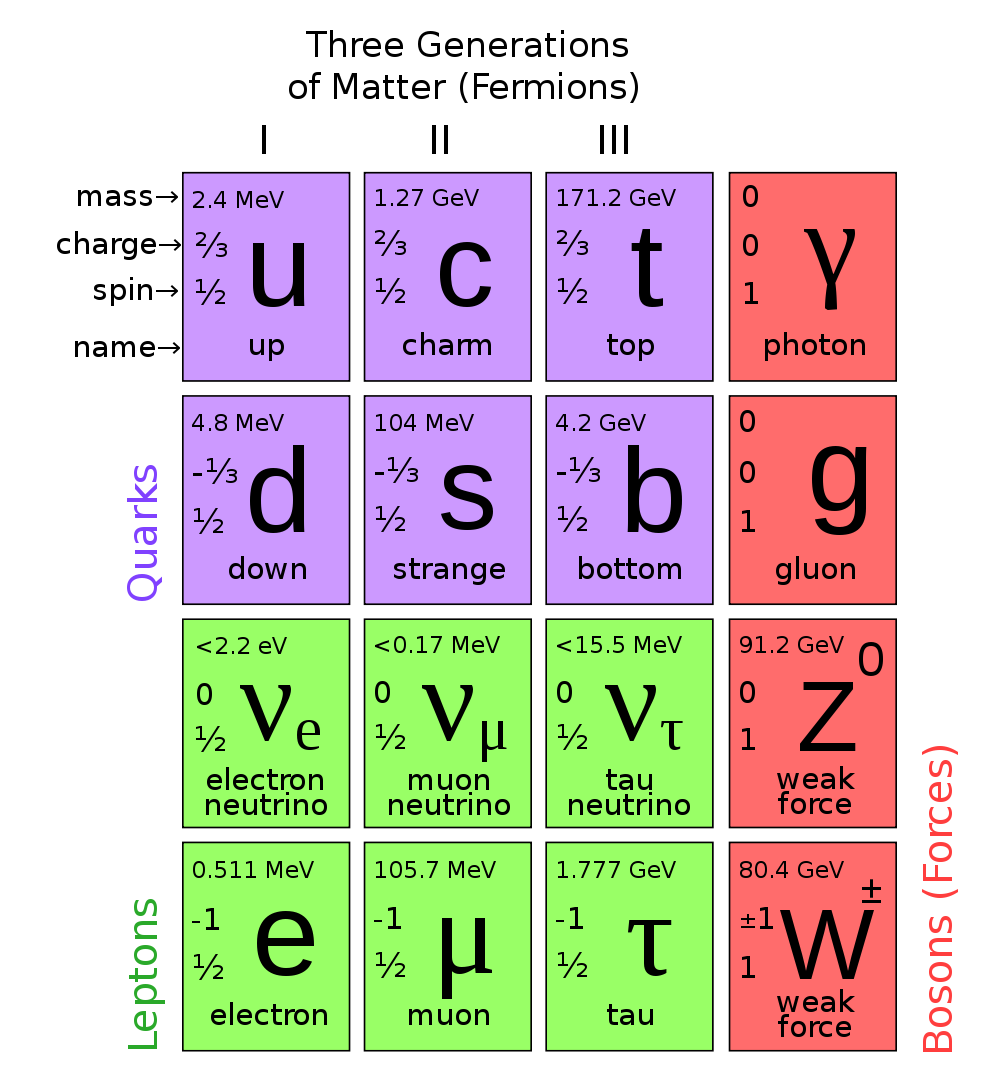
\includegraphics[width=0.6\textwidth]{Introduction/figs/StandardModel3.png}
\caption{Diagram of SM particles with their properties \cite{SMimage}.}
\label{fig:SMparticles}
\end{figure}






\section{Electromagnetic and weak interactions}

The Electromagnetic (EM) force is responsible for binding electrons and nuclei together in atoms.
Its force carrier, the photon, is the gauge boson of the EM force. In the SM the photon must be massless,
which also sets the range of the EM force to infinity, since it is proportional to the inverse of the mediator mass.
In fact Heisenberg's Uncertainty Principle tells us that $\Delta E \Delta t > \hbar$, namely virtual particles
of energy $\Delta E$ are allowed to exist for time intervals inferior to $\Delta t$. Then, since they can move
at maximum at the velocity of light this also sets a relation between the length of time and space in which a virtual
photons can exist. The EM force has an infinite range as virtual photons can be very close to the mass shell, which results
in a very long lifetime.

The weak interaction is responsible for the $\beta$ decay of nuclei and all known fermions interact through the weak
interaction. In the Standard Model of particle physics this interaction is caused by the emission or absorption of $W^\pm$
and $Z$ bosons. These are much heavier than protons or neutrons (see Table \ref{interactions}) and this yields that the weak
force has a very short range. Using Heisenberg's Principle together with Einstein's formula $\Delta E = m c^2$, which relates
mass and energy, and knowing that the maximum space that a particle can cover in a time $\Delta t$ is $r = c \Delta t$,
qualitatively $r \sim \hbar / mc$. In this picture the carriers of the weak force can travel $r \sim 2 \cdot 10^{-3}$ fm.
The weak interaction is also the only one that violates parity-symmetry, which states that interactions are invariant under
a reflection of all coordinates. This symmetry breaking arises from the fact that only left-handed fermions interact through
the weak interaction. The first experiment showing this was made by Wu in 1957 \cite{Wu:1957my}. Similarly, the weak interaction
is the only one that also breaks the CP symmetry, which combines parity transformations and ``charge conjugation".
This is interesting also because all interactions are invariant under CPT transformations, which combines CP transformations
and time reversal, hence, breaking CP the weak interaction is also not invariant under time reversal.

In 1968 Salam, Glasow and Weinberg unified the weak and electromagnetic force in a single theory called electroweak (EW),
having a single coupling constant\cite{PDG2012}. The EW interactions are divided into charged currents (CC) and neutral
currents (NC). In the first group, quarks and leptons interact with the $W^\pm$ bosons, as in the decays
$\mu^+(\mu^-) \rightarrow e^+ \nu_e \bar{\nu_\mu} (e^- \bar{\nu_e} \nu_\mu)$ and $n \rightarrow p e^- \bar{\nu_e} (\bar{p} e^+ \nu_e)$.
The study of these processes confirmed that only the left-handed (right-handed) component of fermions (anti-fermions)
takes part in weak processes. The CC interaction have a peculiarity: they are the only interactions in the SM that violate
flavour conservation at tree level (see next section), while any other interaction not conserving flavour has to happen through
loops. The second group of EW interactions, NC, corresponds to interactions of the photon and $Z$ boson with a fermion
and its anti-fermion.

%The EM theory results from requiring the fermion Lagrangian to be invariant under local gauge transformations.
%The electron and positron free fermionic fields are defined as $\psi(x)$ and $\bar{\psi(x)}$, where x is a relativistic four vector.
%A local gauge transformation can always be written as:
%
%\begin{align}
%\psi(x) \rightarrow \psi(x') = e^i{\alpha(x)}\psi(x)
%\end{align}
%
%where $\alpha(x)$ can be any function of space and/or time. The free fermion Lagrangian, given by
%
%\begin{equation}
%\mathcal{L} = -i \bar{\psi(x)} \gamma^mu \partial_\mu \psi(x) - m\bar{\psi(x)} \psi
%\end{equation}
%
%is not invariant under such transformations. Greek indices denote space-time directions and imply summation and $\gamma^i$ are the Dirac matrices. If we apply the local gauge transformation and we subtract the initial Lagrangian we get a remaining term
%
%\begin{equation}
%\Delta \mathcal{L} = \mathcal{L}' - \mathcal{L} = -i \bar{\psi}  \gamma^mu \psi \partial_\mu \alpha(x)
%\end{equation}
%
%In order to make the Lagrangian invariant we can introduce a vector field $A$, which transforms as described by Eq. \ref{gauge invariance},  to %compensate for the remaining term: this is the photon field.
%
%\begin{equation}
%\label{gauge invariance}
%A'_\mu = A_\mu -\frac{1}{e}\partial_\mu \alpha(x)
%\end{equation}
%
%Redefining then the field derivative $D_\mu = \partial_\mu - ieA_\mu$, we obtain the invariant Lagrangian:
%
%\begin{equation}
%\mathcal{L} = -i \bar{\psi(x)} \gamma^mu D_\mu \psi(x)  - m\bar{\psi(x)} \psi = -i \bar{\psi(x)} (\gamma^mu \partial_\mu  - m)\psi(x) + e\bar{\psi}  \gamma^mu \psi A_\mu
%\end{equation}





\subsection{Flavour and the CKM matrix}

``Flavour" in particle physics refers to the quark/lepton composition of a particle. The introduction of flavour quantum numbers
was motivated in order to explain why some decays, although kinematically allowed, have never been observed. All leptons have a
quantum number $L_l = 1$ (where $l = e,\mu,\tau$), which is conserved by all interactions. For example decays
like $\mu^- \rightarrow e^- \gamma $, which is kinematically possible, have never been observed, since the lepton number
in the initial and final state are different, while decays conserving the lepton number as
$\mu^- \rightarrow e^- \nu_\mu \bar{\nu_e}$ have been observed.

In the non leptonic sector particles carry flavour numbers described as follow:

 \begin{itemize}
 \item \emph{Isospin}: $I_3 = 1/2$ for the up quark and value $I_3 = -1/2$ for the down quark;
 \item \emph{Strangeness}: $S = -(n_s - \bar{n}_s)$, where $n_s$ is the number of strange quarks and $\bar{n}_s$ is the number of anti-strange quarks;
 \item \emph{charmness, bottomness, topness}: in analogy to strangeness
 they are respectively defined as $C = -(n_c - \bar{n}_c)$, $B = -(n_b - \bar{n}_b)$, $T = -(n_t - \bar{n}_t)$.
 \end{itemize}

As mentioned before in the SM the only interaction violating flavour conservation is the weak interaction,
when mediated by $W^\pm$ bosons.

Measuring branching fractions of weak decays like $\pi \rightarrow \mu \nu_\mu$ and $K \rightarrow \mu \nu_\mu$, 
suggested the existence of more than one coupling constant. Cabibbo\cite{PDG2012}, in order to preserve the universality
of weak interactions, suggested that the difference in branching fraction could arise from the fact that
the doublets participating in the weak interactions are a mixture of the flavour eigenstates. He therefore introduced
the Cabibbo angle $\theta_c$ considering that eigenstates participating to the weak interaction are rotated with respect
of the flavour eigenstates.

\begin{equation}
\left( \begin{array}{c}
d_W \\ s_W
\end{array} \right) =
\left( \begin{array}{cc}
\cos \theta_c  & \sin \theta_c\\
-\sin \theta_c & \cos \theta_c
\end{array} \right)
\left( \begin{array}{c}
d \\ s
\end{array} \right) = 
\left( \begin{array}{c}
\cos\theta_c \cdot d + \sin \theta_c \cdot s \\
\cos \theta_c \cdot s - \sin \theta_c \cdot d
\end{array} \right)
\end{equation}

Considering a 6 quark system one angle is not enough to describe a rotation but the mixing system can be generalised
using a $3 \times 3$ unitary matrix, this is called CKM matrix, from the names of Cabibbo, Kobayashi and Maskawa.
The unitarity of the matrix is required in order to conserve the total probability. Theoretically, a $N \times N$ complex
matrix is dependent on $2 \cdot N^2$ real parameters. Then, requiring unitarity ($AA^\dagger = A(A^*)^T = I$),
the number of independent parameters left is $(N - 1)^2$. A $3 \times 3$ depends then on 4 real parameters, which
can be divided in 3 real constants and one imaginary phase. The imaginary phase generates the CP-violation which was
observed in weak interactions. In Eq. \ref{CKM} is reported a parametrisation of the CKM matrix together with the most
recent measured values\cite{PDG2012}. In this parametrisation $\rho$, $A$, and $\lambda$ are the real constants and $\eta$
the imaginary phase; in Eq. \ref{params} are reported their relations with the 3 mixing angles.

\begin{multline}
\label{CKM}
V_{CKM} = \left( \begin{array}{ccc}
1 - \lambda^2/2 & \lambda  & A \lambda^3(\rho -\i\eta) \\
-\lambda & 1 - \lambda^2/2 & A\lambda^2 \\
A \lambda^3(1 - \rho -\i\eta) & A\lambda^2 & 1 
\end{array} \right) + O(\lambda^3)= \\
= \left( \begin{array}{ccc}
0.97427 \pm 0.00015 & 0.22534 \pm 0.00065 & 0.00351^{+0.00015}_{-0.0014} \\
 0.22520 \pm 0.00065 & 0.97344 \pm 0.00016 & 0.00412^{+0.0011}_{-0.0005} \\
 0.00867^{+0.00029}_{-0.00031} & 0.0404^{+0.0011}_{-0.0005} & 0.999146^{+0.000021}_{-0.000046} \\
\end{array} \right)
\end{multline}

\begin{align}
\label{params}
\lambda & = \sin(\theta_{12}) = \sin(\theta_c) \\
A\lambda^2 & = \sin(\theta_{23}) \\
A\lambda^3(\rho - i\eta) & = \sin(\theta_{13})e^{i\delta}
\end{align}

It is interesting to note that the CKM matrix seems to be hierarchical, namely elements on the diagonal are approximately
1 and then get smaller and smaller going farther from the diagonal.
An other feature to note is that, due to the unitarity of the matrix, the transformation have no effect on neutral interaction.
As a result flavour-changing neutral currents are forbidden at tree level (in absence of closed loops) in the SM.

The CKM matrix to preserve probability has to be unitary and this imposes constraints to its terms for the form:
\begin{equation}
\sum_i |V_{ik}|^2 = 1 \text{ and } \sum_k V_{ik} V^{*}_{jk} = 0.
\end{equation}
This is a contraint of 3 complex numbers that can be viewed as the sides of a triangle called
the ``unitarity triangle". The precise measurement of the parameters of the unitarity triangle
is a powerful stability test of the standard model and sets a solid base for new physics
searches in the favour sector.

In Fig.~\ref{fig:unitarity_triangle} is shown a representation
of the unitarity triangle together with a plot summarising the most up to date contraints
the the angles from measurements. One of the main goals of the LHCb experiment is to precisely
measure the angle $\gamma$, which is currently the least constrained from measurements.
 
 \begin{figure}[h!]
\label{fig:unitarity_triangle}
\centering 
\includegraphics[width=0.8\textwidth]{Introduction/figs/Unitarity_triangle.png}
\includegraphics[width=0.8\textwidth]{Introduction/figs/Unitarity_triangle_HFAG.png}
\caption{(left) A representation of the unitarity triangle and its parameters.
(right) A summary of the most up to date measurements of the unitarity triangle parameters \cite{}.}
\end{figure}
 
 
 
 
\section{The puzzles in the SM}
\label{SMproblems}
Despite the confirmation of many predictions of the SM, this theory has several limitations and is unable to account for some observational facts.

\begin{itemize}
\item \emph{Dark matter}: From experimental evidence the content of visible matter in the universe is not enough
to account the observed rotation of galaxies \cite{Zwicky:1933gu} in the context of general relativity. 
Furthermore, studies of the fluctuations of the cosmic microwave background indicate the existence of
cold dark matter\cite{Dunkley:2008ie}, formed of particles which do not interact through the SM forces and
for which there is no SM candidate.

\item \emph{Matter-antimatter asymmetry}: We observe a large asymmetry between the quantity of matter and antimatter
in the Universe. Assuming that both were equally created in the initial state of the Universe, a condition such
as the violation of the CP symmetry is necessary to account for such observed differences. However the magnitude of
CP violation predicted by the SM is not enough to explain them \cite{Gavela:1993ts}.

\item \emph{Gravity}: There is not yet a consistent procedure to introduce gravity in the SM.

\item \emph{Neutrino oscillation}: By now, many measurements regarding solar and atmospheric neutrinos as wells as
neutrinos from nuclear reactor established that neutrinos can change flavour while propagating in space.
This is not predicted in the SM, in fact in the SM neutrinos are massless while an oscillation requires a non
zero mass \cite{Maltoni:2011zz}.

\item \emph{The mass hierarchy problem}: The mass of a scalar (spin 0 particle), such as the Higgs boson,
suffers from quantum corrections of its mass due to the physics above a certain scale
$\Lambda$, $m^2_{HSM} (phys) \sim m^2_{HSM} +  \frac{c}{16\pi}\Lambda^2$. Using the recently measured value
for the Higgs mass $\sim 126 ~\mbox{GeV/c}^2$\cite{Filippis:2013ana}, $\Lambda$ should be $\sim TeV$ in order
to avoid a fine tuning of the bare mass term.

\end{itemize}

\subsection{The flavour problem}

The SM has been very successful in describing the observed particles and their interactions so far. However, because
of its many puzzles, described in \ref{SMproblems}, it is believed only to be part of a more general theory or only
to be valid up to a certain energy scale. Many theoretical models expect New Physics (NP) to enter at the TeV scale.
For example, flavour conservation does not have a strong theoretical basis in the Standard Model and is mainly motivated
by experimental evidence.

So far we have talked about Flavour Changing Charged Currents (FCCC) that are mediated by the $W^\pm$ bosons. In the SM,
they are the only sources of flavour changing interaction and, in particular, of generation changing interactions,
where a quark or a lepton of a family transforms into one of an other family. There is no fundamental reason why there
cannot be Flavour Changing Neutral Currents (FCNCs). Yet, experimentally we see that FCNCs processes are highly suppressed.
The way in which the SM explains this is to forbid FCNC at tree level: since $Z$ and $\gamma$ interaction conserve flavour
the only other way to have FCNC is through particle loops. This makes this interactions very sensitive to new physics,
since its effects, which are expected to be small, are not disguised by dominating SM processes.

By now one of the possible explanations why we do not observe FCNC at tree level is the Minimal Flavour Violation (MFV)
hypothesis\cite{Isidori:2012ts}\cite{Buras:2003jf}, where FCNC are 'protected' by symmetry principles.


\section{Beyond the Standard Model}

From the last two sections it is evident that, despite the great success of the SM,
there is a need to explote new theories. Among the most promising approaches are those
invoking Super-Symmetry and extradimensions 

In Super-Symmetry new degrees of freedom are introduced to suppress the diverging term of the scalar mass. This represents
the main reasoning of Super-Symmetry, which assumes that for each fermion there is a corresponding boson. Since boson and
fermions contribute with opposite sign to the mass term they would cancel out if for each fermion we can add a boson term
\cite{Fayet:1976cr}.

The idea to introduce extra dimensions was triggered by the fact that normally gravity is not relevant
in particle physics at today's energy scales, which is at the EW scale ($\sim 100$ GeV), and this is why
it is neglected in the SM. However, adding extra dimensions to the normal 3 spatial dimensions,
one can restore some of the strength of gravity, yielding effects at the EW scale \cite{Randall:1999ee}.

In all these approaches severe contraints on masses and couplings must be imposed to maintain
compatibility with the SM at the electroweak scale.

\section{Flavour and BSM theories}

Since most of the BSM theories predict processes violating flavour, the observation or non-observation
of these processes can give important information about New Physics.

BSM theories can be classified according to the amount of flavour violation they introduce.
The first class of models to consider is the Minimal Flavour Violation (MFV).
These are models where the only sources of flavour violation in the SM and in BSM
are the different Yukawa couplings.
The MFV paradigm provides a way to resolve the tension between expectation, driven by naturalness arguments,
that NP should be at the \tev scale and limits on FCNC processes that point to much higher scales.
As hamiltonians for $\bquark\to\dquark$ and $\bquark\to\squark$ share the same structure,
ratios between these transitions provide powerful tests of MFV.
One particularly important example is the ratio of $\Bz$ and $\Bs$ dimuon decay rates \ref{}.

In the quest fot New Physics an important role is also played by simplified models
as a intermediate model building step. Instead of building models valid up to the GUT scale
one could consider simplified models including the SM and a new sector with a limited number
of parameters. Such models are easier to constrain but can nevertheless point in the right direction
to build a complete theory. The choice of the new sector to add can be driven by the need to
explain existing discrepancies between data and SM predictions or by theoretical prejudice.

Two models especially relevant for the discussion in this thesis are Z'-penguins and leptoquarks.

A Z'-penguin is a FCNC process involving a neutral field and as for the SM penguins it arises in
loops and modifications of the effective couplings arise in most SM extensions.
A survey of Z' models can be found in Ref. \cite{}.

Leptoquarks are bosonic particles that carry one quark and one lepton flavour quantum number.
They can be spin 1 but they ar more commonly assumed to be scalar particles.
A three level exchange of these particles induces processes such as $\bquark \to (\squark,\dquark)\ell\ell$
ans therefore we could observe an enhancement of their decay rates with respect to the SM.
Leptoquarks also provide a natural explanation for non-universal couplings to leptons,
introducing lepton flavour violation.


\section{Rare decays: a tool to search for new physics}

In the SM Flavour Changing Neutral Current processes, e.g. transitions from a
\bquark quark with charge of 1/3 to a \squark or \dquark with a charge of +2/3, 
are forbidden at tree level but can occur trough loops, box or penguin decays, see Fig.~\ref{fig:penguins}.
The branching fractions of this kind of decays is $\sim 10^{-6}$ or lower and therefore
they are called "rare decays". Additional NP contributions to the virtual loops
are not necessarily suppressed with respect to the SM component and this makes these decays
very sensitive to New Physics. Furthermore, this approach to New Physics searches is interesting as
New Physics could be at a high mass scale not accessible at colliders but its effect could be observed in loop effects.
Radiative and penguin decays are particularly interesting because they are theoretically
well understood which allows precise comparisons with measurements. Finally they provide
a great quantity of observables, not only decay rates, but also CP asymmetries and
angular observables can be affected by New Physics.

\begin{figure}[h!]
\centering
\includegraphics[width=0.8\textwidth]{Introduction/figs/penguins3.png}
\caption{Loop Feynmann diagrams for the rare $b \rightarrow s $ decay.}
\label{fig:penguins}
\end{figure}

\subsection{Theoretical framework: the effective Hamiltonian}
\label{sec:Effective_Hamiltonian}

Rare B decays are governed by an interplay between weak and strong interactions.
The QCD corrections that arise from hard gluon exchange bring large logarithms
of the form $\alpha_s^n(m_b)\log^m(m_b/M)$, where $M = m_t$ or $M = m_W$.
%A suitable framework to achieve the necessary resummation of these logarithms
%in an effective low-energy theory with five quarks.
The large masses of W, Z and top quark compared to that of the \bquark quark allow
the construction of an effective low-energy theory where the effective hamiltonian
can be written as:

\begin{equation}
\mathcal{H}_{eff} = \frac{4G_F}{\sqrt{2}} \sum C_i(\mu,M)\mathcal{O}_i(\mu)
\end{equation}

The method of the Operator Product Expansion (OPE) allows the separation
of the decay amplitudes into two parts: the long-distance contributions,
contained in the operator matrix elements, $\mathcal{O}_i$, and the short-distance physics described
by the so called Wilson Coefficients, $C_i$. $G_F$ denotes the Fermi coupling constant.

The weak coefficients at the weak scale can be obtained from matching amplitudes
of the full electroweak theory into $\mathcal{H}_{eff}$.
Then one can derive a renormalization group equation for the Wilson Coefficients

\begin{equation}
\mu \frac{\deriv}{\deriv \mu} C_i(\mu) = \gamma_{ij}C_j(\mu)
\end{equation}

where the matrix $\gamma$ is the anomalous dimensions matrix of the operators $\mathcal{O}_i$.
At leading order the solution is given by:

\begin{equation}
C_i(\mu) = \left[ \frac{\alpha_s(\mu_W)}{\alpha_s(\mu)}\right]^{\frac{\gamma^0_{ii}}{2\beta_0}} C_i(\mu_W) = \left[ \frac{1}{1 + \beta_0\frac{\alpha_s(\mu)}{4\pi}ln\frac{\mu_W^2}{\mu^2}} \right]^{\frac{\gamma^0_{ii}}{2\beta_0}} C_i(\mu_W)
\end{equation}

\subsection{Perturbative corrections}

The relevant efective Hamiltonian for $\bquark\to\squark\ell^+\ell^-$ transitions is

\begin{equation}
\mathcal{H}_{eff} = \frac{4G_F}{\sqrt{2}} \left[ V_{tb}V^*_{ts} \sum_{i=1}^{10} C_i \mathcal{O}_i \right]
% + V_{ub}V^*_{bs} \sum_{i=1}^{2} C_i ( \mathcal{O}_i - \mathcal{O}_i') \right]
\end{equation}

where the $V_{ub}$ and $V_{bs}$ are the factors of the CKM matrix.
The following local operators are particularly important for leptonic decays:

\begin{align}
& \mathcal{O}_7 = \frac{m_b}{e} \bar{s} \sigma^{\mu\nu}P_RbF_{\mu\nu}  			& \mathcal{O}_7' = \frac{m_b}{e} \bar{s} \sigma^{\mu\nu}P_LbF_{\mu\nu} \\
& \mathcal{O}_8 = g_s\frac{m_b}{e} \bar{s} \sigma^{\mu\nu}P_RT^abG^a_{\mu\nu}  	& \mathcal{O}_8' = g_s\frac{m_b}{e} \bar{s} \sigma^{\mu\nu}P_LT^abG^a_{\mu\nu} \\
& \mathcal{O}_9 = \bar{s} \gamma_{\mu}P_Lb\bar{\ell}\gamma^\mu\ell  			& \bar{s} \mathcal{O}_9' = \gamma_{\mu}P_Rb\bar{\ell}\gamma^\mu\ell \\
& \mathcal{O}_{10} = \bar{s} \gamma_{\mu}P_Lb\bar{\ell}\gamma^\mu\gamma_5\ell 	& \mathcal{O}_{10}' = \bar{s} \gamma_{\mu}P_Rb\bar{\ell}\gamma^\mu\gamma_5\ell \\
\end{align}


where $P_{L/R} = (1 \mp \gamma_5)/2$ denotes the left/right handed chiral projection,
$T^a$ are the QCD generators and $F_{\mu\nu}$ is the elecromagnetic field tensor.
The $\mathcal{O}'$ operators correspond to right-handed coupling obtained by swapping $P_R$ and $P_L$ in the equations.
The left-handedness of the weak interaction means that the $C'$ Wilson Coefficients are suppressed by $O(m_s / m_b)$ in the SM.

In the SM at $\mu_s = m_b$ the Wilson Coefficients have values:

%\begin{equation}
\begin{align}
& C_7^{SM} = -0.3, & C_9^{SM} = 4.2, & C_{10}^{SM} = -4.2. \\
\end{align}
%\end{equation}

New Physics contributions appear in the Wilson Coefficients as additive factors $C_i = C_i^{NP} + C_i^{SM}$

\subsection{Phenomenology of $\bquark\to\squark\ell\ell$ decays}
\label{sec:theo_qsq}

\begin{figure}[h!]
\centering
\includegraphics[width=0.8\textwidth]{fig/q2spectrum.png}
\caption{A typical $q^2$ spectrum of $\bquark\to\squark\ell\ell$ process characterised by the photon pole
at very low \qsq, charmonium resonances at central \qsq and broad resonances at high \qsq.}
\label{fig:q2spectrum}
\end{figure}

Semileptonic \bquark hadron decays are characterised by two kinematic regimes: at low \qsq, where the emitted hadron
is energetic ($E > \Lambda_{QCD}$ in the \bquark hadron rest frame), QCD factorisation applied; at high \qsq, the region
of low hadron recoil ($\qsq = O(m_b)$), an Operator Product Expansion (OPE) in $1/m_b$ applies.
In both regions decays can be predicted using the different methods and the biggest uncertainties come
from the limited knowledge of hadronic transition from factors.

As can be seen in Fig.~\ref{fig:q2spectrum} at very low \qsq the virtual photon contribution, associated with $C_7$, dominates.
In the region $1-6$ \gevgevcccc the interference between $C_7$ and $C_9$ becomes large, yielding sensitivity to NP in $C_9$.
The $6-15$ \gevgevcccc interval is dominated by charmonium resonances, \jpsi and \psitwos, though the tree level $b\to\cbar c s$ transition.
Although the decays can be experimentally vetoed in principle charmonia affect the entire \qsq space. 
Finally, at high \qsq borad charmonium resonances can contribute, like those observed by LHCb in $\decay{B^+}{K^+\mumu}$ decays \cite{}.

\subsection{Observables in $\bquark\to\squark\ell\ell$ decays}
\label{sec:observables}

Rare decays and especially semileptonic $\bquark\to\squark\ell\ell$ processes offer a pletora
of observables which can be used to search for New Physics.
The most direct effects appear in decay rates that can be enhanced by NP but the precision on
these measurements is often by uncertainty of form factor calculations or charm loops.
Therefore it is important also to look for different observable.
One important class of observables are angular quantities that can carry information about NP,
often complementary to branching ratio measurements. The most basic of these observable are
forward-backward asymmetries that characterise the angular distribution of final particles.
For the \Bz\to\Kstar\mumu decay combination of observables have been proposed that are 
independent of form factor uncertainties in the fits order \cite{}.
One more way to build stable observable is t/o construct ratios between similar
decays in which, for example, uncertainties due to the hadronisation process cancel out.
These observables include the $R_H$ ratios, between \Bz decay into electrons and muons,
that are described in detail in Sec.~\ref{sec:RKst_theory}.


\section{Experimental status}

In order to set the background for the searches included in this thesis, in this section a review of recent
or important results of NP searches involving rare decays or lepton flavour violation.
Among these, results recently obtained by the \lhcb experiment show a series of anomalies
with respect to the SM that have the potential to yield to NP scenarios.


\subsection{Dimuon decays of \bquark hadrons}

Decays of $B$ mesons into two muons have been recently studies at the \lhcb and \cms experiments.
These are two-body decays where the two muons are back to back in the hadron rest frame.
The simple signatures of these decays makes them easy to study and the fact that they
are unaffected by hadronic physics in the final state makes predictions very clean and precise.
Therefore these are essential tests for the SM.
The $\decay{\Bz}{\mumu}$ and $\decay{\Bz}{\mumu}$ decays are exceedingly rare in the SM.
First of all they can only happen in loops and furthermore they are CKM-suppressed.
In addition to that the decay of a pseudo-scalar $B$ meson into two muons has a significant helicity suppression.
The latest SM predictions for these decay rates are \cite{}:
%
\begin{align}
\mathcal{B}(\decay{\Bs}{\mumu}) = (3.65 \pm 0.23) \times 10^{-9} \text{ and } \\
\mathcal{B}(\decay{\Bz}{\mumu}) = (1.06 \pm 0.09) \times 10^{-10}.
\end{align}
%
The uncertainties on these values mainly comes from the knowledge of the decay constants and CKM-elements.
BSM models, for example models with extended Higgs sectors can produce significant enhancement to
these decays. Furthermore the measurement of their ratio is a stringent test of the MFV hypothesis.
A combination of the \lhcb and \cms results resulted in the measured values \cite{}:
%
\begin{align}
\mathcal{B}(\decay{\Bs}{\mumu}) = (2.8^{+0.7}_{-0.6}) \times 10^{-9} \text{ and } \\
\mathcal{B}(\decay{\Bz}{\mumu}) = (3.9^{+1.6}_{-1.4}) \times 10^{-10}.
\end{align}
%
Both decays where unobserved and now the $\Bs$ decay was observed with a significance of $6\sigma$
and evidence for the $\Bz$ decay was found with a $3\sigma$ significance.
These are compatible with SM predictions within $2\sigma$ and put strong contraints to
the available parameter-space for BSM theories.

\subsection{Semileptonic $\bquark\to\squark\ell\ell$ decays of \bquark hadrons}

Many branching ratios of semileptonic $B$ meson decays where recently measured at the \lhcb experiment,
including $\decay{B}{K\mumu}$, $\decay{B}{K*\mumu}$ and $\decay{\Bs}{\phi\mumu}$ \cite{}.
Baryon decays where also studied at \lhcb: including the branching ratio of
the rare $\decay{\Lambda_b}{\Lz\mumu}$ decay \cite{}, which is described in this thesis.
For semileptonic decays, unlike for dilepton decays, SM predictions are affected by the
knowledge of hadronic form factors, {\em describing phsycis bla bla}. This typically yields
to uncertainties of $\mathcal{O}(30\%)$.
As described in \ref{sec:observables} many observables can be affected by 


\subsection{Lepton Flavour Violation searches}

Several LFV searches are linked to rare decays as they involve small branching ratios
in the SM that can be enhances by NP. They are therefore a natural place to look for NP.
Lepton flavour conservation is well experimentally established but has no strong theoretical explanation
and in fact we already know that flavour is not conserved in neutrino oscillations.
In this section is reported a short review of Lepton Flavour Violation searches.
The best-studied decays violating lepton flavour are rare muon decays including $\mu^+\to e^+\gamma$
and $\mu^+\to e^+e^-e^+$. Since muons can be abundantly produced and the final states are simple,
these decays provide the best constraints to LFV. The present best-upper limits are $1.2 \times 10^{-11}$
for the radiative decay and $1.0 \times 10^{-12}$ for $\mu^+\to e^+e^-e^+$ obtained respectively by the
MEGA \cite{} and SINDRUM \cite{} experiments.

Several LFV searches have been recently been performed at the LHCb experiment including $B$ meson
decays such as $\Bz\to e\mu$ \cite{} and $\tau$ decays such as $\tau\to\mumu\mu$ \cite{}.
None of these searches has found evidence of NP so far and therefore they set limits, constraining
the parameter space available for NP models. Fig.~\ref{fig:LFV_decay} reports a summary of
the best limits on LFV searches.


\begin{figure}[h!]
\label{fig:LFV_decay}
\centering 
\includegraphics[width=0.8\textwidth]{Introduction/figs/LFV.png}
\caption{Summary of limits set in lepton flavour violation searches \cite{}.}
\end{figure}
 

\chapter{The LHCb detector at the Large Hadron Collider}
\label{ch:detector}

\section{The Large Hadron Collider}

The Large Hadron Collider (LHC)~\cite{Evans:2009zzc} is a synchrotron particle accelerator with a circumference 
of 27~km located about 100~m underground at CERN in the surroundings of Geneva, Switzerland. 
Two proton beams circulate in opposite directions around the ring and cross each
other in four points, in which particle detectors are placed. These include two general-purpose detectors, 
ATLAS and CMS, sitting on opposites sides of the ring and two smaller detectors, 
ALICE and LHCb that are designed to study specific topics (see Fig.~\ref{fig:lhc}).

\begin{figure}[h!]
\centering
\includegraphics[width=1\textwidth]{Detector/figs/LHC_scheme.png}
\caption{Schematic of CERN accelerators.} 
\label{fig:lhc}
\end{figure}

Each beam consists of a series of proton bunches, up to a maximum of 2835. Each bunch consists of about $10^{11}$
protons and the bunch spacing is such that the nominal bunch crossing rate is 40 MHz. The beams are injected into
pre-accelerators and then pass into the LHC through the CERN acceleration system shown in Fig.~\ref{fig:lhc}. Protons are
produced from hydrogen gas and are initially accelerated to an energy of 50 MeV in a linear accelerator (LINAC).
Then they are injected into the Proton Synchrotron Booster (PSB), where they are boosted to an energy of 1.4 \gev,
into the Proton Synchrotron (PS) to 25~\gev~and into the Super Proton Synchrotron (SPS) to 450~\gev. Finally, protons
enter into the LHC storage ring, where they are accelerated from injection energy to the final one
by radio frequency (RF) cavities. The beams are steered around the ring by 8~T magnetic fields produced by 15~m long
superconducting niobium-titanium dipole magnets and focused by quadrupole magnets. The LHC magnets
use a design in which both proton beam pipes are contained in the same housing, allowing a common liquid helium cooling
system to be used. The LHC began colliding proton beams in ``physics mode" in 2009 at a centre of mass
energy of $\sqrt{s} = 900$~\gev~and from April 2010 to November 2011 accelerated beams at $\sqrt{s} = 7$~\tev~(3.5~\tev~per
proton beam) with a maximum instantaneous luminosity of $3\cdot10^{33} \text{ cm}^{-2}\text{s}^{-1}$, while in
2012 the energy was increased to 8~\tev. The LHC maximum design energy is 14 TeV, and its design
luminosity is $10^{34} \text{ cm}^{-2}\text{s}^{-1}$. After a long shut down to upgrade and maintain the machine, a
new run started in June 2015, in which protons are collided at a centre of mass energy of $\sqrt{s} = 13$~\tev. At this
energy the total proton-proton cross-section is expected to be roughly 100 mb.
%, thus at the design luminosity the general purpose detectors will an event rate approximately $10^9$ inelastic events/s.

\section{The LHCb detector}

The LHCb detector~\cite{Alves:2008zz} was designed to study decays of $B$ and $D$ mesons,
mainly looking for CP-violating processes. In 2011, running at a centre of mass energy of 7 TeV, 
the cross-section for $b\bar{b}$ production was measured to be $284 \pm 53 ~\mu$b~\cite{Aaij:2010gn}, 
while it will be $\sim500 ~\mu$b at the current LHC energy, 13 TeV.
At these high energies, proton-proton interactions produce highly boosted virtual gluons which produce $b\bar{b}$
pairs at small angles, close to the beam pipe. For this reason the LHCb detector is designed to have a very forward angular
coverage. The detector is fully instrumented from 10 mrad to 300 mrad, corresponding to an interval
$2 < \eta < 5$, where $\eta$ is the ``pseudorapidity", a quantity defined as:
\begin{equation}
\label{pseudorap}
\eta = - \ln(\tan(\theta/2)),
\end{equation}
where $\theta$ is the angle between a particle's momentum and the beam direction\footnote{LHCb's reference 
system has the $z$ axis in the direction of the beam, the $x$ axis directed to
the centre of the accelerator and $y$ is directed upward. Then we define $\theta$ as the angle with the beam
direction and $\phi$ as the position around the beam in the $xy$ plane, taking $\phi = 0$ on the $x$ axis.
The origin, $(x,y,z)=(0,0,0)$, corresponds to the centre of the interaction area.}.

\begin{figure}[h]
\includegraphics[width=1.\linewidth]{Detector/figs/LHCb_official.png}
\caption{A side view of the LHCb detector~\cite{Alves:2008zz}.}
\label{fig:lhcb}
\end{figure}

At LHCb's collision point the luminosity can be adjusted by displacing the beams from head on collisions
while keeping the same crossing angle. This allows the experiment to keep an approximately constant instantaneous
luminosity, compensating for the reduction in beam intensity due to extended operation periods. This also means that
the average number of interactions per bunch crossing can be regulated, which is important
because the detector efficiency, especially in detecting secondary vertices, decreases for events with an high number
of primary vertices (PV). Reducing the particle occupancy through the detector also keeps radiation damage to a minimum. 
Until the end of 2011 the instantaneous luminosity was $3 \cdot 10^{32}~\mbox{cm}^{-2}\mbox{s}^{-1}$, corresponding 
to an average number of 1.5 PVs per bunch crossing and at the end of 2011 LHCb had collected an integrated
luminosity of 1~\invfb. In 2012 the luminosity was increased and a further 2~\invfb of data were collected.

Experiments like BaBar at the Stanford Linear Accelerator (SLAC), Belle at KEK at J-PARC (Japan)
and the Tevatron experiments at Fermilab have made measurements in heavy flavour physics
which have so far been found to be consistent with the SM predictions. However, some of the deviations from the
SM are expected to be very small. Therefore LHCb was designed to make the most precise measurements
in heavy flavour physics to test the consistency of the SM and look for new physics.

The LHCb detector includes a high-precision tracking system consisting of a silicon-strip
vertex detector surrounding the $pp$ interaction region, and a larger silicon-strip and drift tubes detectors located
on both sides of a dipole magnet with a bending power of about 4~Tm.
%The combined tracking system has momentum resolution $\Delta p/p$, that varies
%from 0.4\% at 5 $\mbox{GeV/c}^{2}$ to 0.6\% at 100 $\mbox{GeV/c}^{2}$. 
Charged hadrons are identified using two
Ring-Imaging Cherenkov detectors (RICH)~\cite{LHCb-DP-2012-003}. Photon, electron and hadron candidates are
identified by a calorimeter system and muons by a system composed of alternating layers of iron
and multi-wire proportional chambers~\cite{LHCb-DP-2012-002}. A schematic view of the detector is shown in Fig.~\ref{fig:lhcb}
and more details on each sub-detector are given in the following sections.

\section{The magnet}

Charged particle trajectories are deflected horizontally in the magnetic field
so that their momentum can be measured from the radius of curvature.
The LHCb dipole magnet is composed of two coils supported by an iron yoke
and is shaped to fit the LHCb angular acceptance. Unlike the other LHC experiments,
LHCb uses a warm magnet which can be easily ramped allowing the field polarity to be inverted periodically.
When the polarity is flipped, particles of a given sign are bent in the opposite direction.
This method is used to limit systematic uncertainties that arise due to performance
variations in different areas of the detector, which average out using data taken in both polarities.
A current of 5.85~kA flows in the magnet generating an integrated magnetic field of 4~Tm for 10~m long tracks.
In order to achieve the required momentum precision the magnetic field must be mapped with
a $10^{-4}$ precision. For this reason a grid of 60 sensors is positioned inside the magnet
and provides real time magnetic field maps.

\section{Tracking system}
\label{sec:tracking}

$B$ mesons have lifetimes of approximately 1.5 ps. At the LHC energies, this means that they travel about
1~cm before decaying to form a displaced vertex. To study specific decays, it is therefore important
to be able to separate the particles produced at the primary $pp$ vertex and at the $B$ decay secondary vertex (SV).
The tracking system consists of the Vertex Locator (VeLo), and four tracking stations:
the Tracker Turicensis (TT), which are located before the magnet and the T1, T2 and T3 stations,
located after the magnet. The latter three stations are in turn formed by two subsystems:
the Inner Tracker (IT) close to the beam-line, where the particle density is greatest, and
the Outer Tracker (OT) covering the rest of the acceptance.
%
\begin{center}
\begin{figure}[h!]
\centering 
\includegraphics[width=0.49\textwidth]{Detector/figs/detector/VELO.png}
\includegraphics[width=0.49\textwidth]{Detector/figs/detector/VELO_scheme.png}
\caption{On the left VeLo sensors mounted in line and on the right a schematic view of one sensor~\cite{Alves:2008zz}.}
\label{VeLo}
\end{figure}
\end{center}
%
The VeLo accurately measures positions of tracks close to the interaction point which is essential to reconstruct
 production and decay vertices of bottom and charm hadrons. The VeLo is composed by 21
silicon modules that surround the beam axis and are positioned from $z = -18$~cm to $+80$~cm.
The sensitive region of the VeLo starts at an inner diameter of only 8~mm from the beam axis and it is able
to detect particles within a pseudorapidity range $1.6 < \eta < 4.9$. The VeLo is housed in its own
vacuum vessel of thin aluminium foil, which protects the vacuum of the beam pipe from any outgassing. 
The silicon layers composing the VeLo consist of two modules each including two types of sensors:
the $\phi$-sensor, which measures the azimuthal position around the beam, and the R-sensor, which measures
the radial distance from the beam axis. A sketch of the VeLo sensors is shown in Fig.~\ref{VeLo}. The sensors
are 300 $\mu$m thick and to ensure that they cover the full azimuthal angle the right-side module is placed
1.5~cm behind the left-side module on the $z$-axis and they overlap. There are two modules which cover the
backward direction and are used as a veto for multiple interactions; this is called the pileup system.
%
\begin{center}
\begin{figure}[h!]
\centering 
\includegraphics[width=0.8\textwidth]{Detector/figs/straw_tubes.png}
\caption{A sketch of the straw tubes which constitute the OT layers~\cite{Alves:2008zz}.}
\label{fig:straw:tubes}
\end{figure}
\end{center}
%
The IT and TT both use silicon strips and together constitute the Silicon Tracker (ST). Straw tubes are instead used 
in the OT, of which a sketch is shown in Fig.~\ref{fig:straw:tubes}. The IT requires a higher inner granularity
because of the greater flux of particles close to the beam pipe. In fact, it covers only 1.3\% of the total
area of IT plus OT but it contains about 20\% of the tracks. Each ST station has four detection layers:
the first and last are vertical, measuring the track position in $x$, while the second 
and third layers are rotated by an angle of +5 and -5 degrees, which allows the measurement of the $y$ coordinate. 
The TT is placed upstream of the magnet to allow the reconstruction of tracks from low-momentum particles,
which are bent out of the downstream acceptance. Overall the tracking system provides a measurement of momentum, 
$p$,  with a relative uncertainty that varies from 0.4\% at 5~\gevc~to 1.0\% at 200~\gevc. 
The impact parameter (IP), namely the minimum distance of a track to a primary vertex, is measured 
with a resolution of $(15 + 29/\pt)$~$\mu$m, where \pt is the component of the momentum transverse to the 
beam, in \gevc. The $z$-axis position of a PV reconstructed with 35--40 tracks can be measured with a precision 
of roughly 50--60~$\mu$m. The decay products of $B$ mesons tend to have high IP values because the B decay imparts
transverse momentum to them. Therefore, accurate IP and vertex displacement measurements allow LHCb to distinguish 
effectively between $B$ meson decays and background processes. 
%In fact $B$ mesons typically travel $\sim 1$ cm in
%the detector before decaying into lighter particles, which .


\section{Calorimeters}
\label{sec:calorimeters}

In general the main purpose of a calorimeter system is to determine the energy of particles
but in LHCb it is mostly used to help the identification electrons and hadrons. 
Sampling calorimeters, as those used in LHCb, are composed of layers of absorber and active material.
Particles interact with the absorber layers and produce a cascade of secondaries, that multiply quickly and are detected by the active part,
which is usually composed of scintillating layers. The light produced is detected by photo-multipliers (PMTs) and it is approximately
proportional to the energy of the deposited particles. Calibration is then used to translate the signal into an energy measurement. 
The LHCb's calorimeter system consists of the Scintillator Pad Detector (SPD), the Pre-Shower Detector (PS)
as well as the Electromagnetic Calorimeter (ECAL) and the Hadronic Calorimeter (HCAL).
A sketch of the LHCb calorimeters is shown in Fig.~\ref{fig:pi0_e_pid_perf}. 
The SPD/PS cells are read out with PMTs located outside the LHCb acceptance, while the ECAL and HCAL
have individual PMTs located on the modules. All four detectors are segmented, which allows the energy
deposits to be associated to the tracks detected by the tracking system. The segmentation of the cells
varies according to the distance from the beam pipe due to the different track density.

The most difficult identification in LHCb is that of electrons. The rejection of a high background of charged pions
is achieved using a longitudinal segmentation of the electromagnetic calorimeter which is provided by
the PS detector added in front of the main electromagnetic calorimeter, ECAL. Electrons also have to be 
distinguished from high energy $\pi^0$s and photons. For this purpose the SPD calorimeter, detecting charged particles,
is located in front of the PS and ECAL detectors. Figure~\ref{fig:pi0_e_pid_perf} illustrates how the ratio between the
energy detected in the ECAL and a particle's momentum allows the separation of electrons and hadrons.

\begin{figure}[t!]
\centering
\includegraphics[width=0.4\textwidth,height=5.3cm]{Detector/figs/pi0_e_pid_perf.png}
\includegraphics[width=0.59\textwidth]{Detector/figs/calo_layout.png}
\caption{(left) The ratio of the energy deposited in the ECAL and the particle momentum, which allows
the separation between electrons and hadrons~\cite{Alves:2008zz}. (right) A schematic of the LHCb's calorimeter system. }
\label{fig:pi0_e_pid_perf}
\end{figure}

The ECAL is formed by 66 lead layers (2 mm thick) separated by 4 mm thick plastic scintillator layers.
In order to obtain the highest energy resolution the showers from high energy photons 
must be fully absorbed. For this reason the ECAL has a thickness of 25 radiation lengths and its resolution is 
measured to be $\sigma_{\rm ECAL}(E) / E = 10\% / \sqrt{E(\gev )} + 1\%$~\cite{Alves:2008zz},
which results in a mass resolution of $\sim 70$ \mevcc~for $B$ mesons and $\sim 8$ \mevcc~for \piz.
The HCAL is mainly used for triggering and it is similar to the ECAL but with 4 mm thick scintillator layers and 
16 mm thick absorber layers. The trigger requirements on the HCAL resolution do not depend on the containment of the hadron showers
as much as for the ECAL, therefore, due to space limits, its thickness is only 5.6 interaction lengths and its resolution is given by
 $\sigma_{\rm HCAL}(E) / E = 69\%/\sqrt{E(\gev )} + 9\%$.

\subsection{Bremsstrahlung recovery for electrons}

Bremsstrahlung is an electromagnetic radiation produced by charged particles that undergo an acceleration. 
%because of the presence other charged particles. 
Typically electrons produce Bremsstrahlung when deflected by atomic nuclei.
The probability of emitting bremsstrahlung radiation is proportional to the inverse of the squared mass of the
particle ($1/m^2$) and therefore it is most relevant for electrons.
%
\begin{figure}[h!]
\centering
\includegraphics[width=0.55\textwidth]{RKst/figs/brem_recovery.png}
\caption{Schematic view of the bremsstrahlung recovery~\cite{Alves:2008zz}. }
\label{fig:bremreco}
\end{figure}
%
At LHC energies, if electrons radiate after the magnet, the photon will hit the same calorimeter cell
 as the electron and the energy will be automatically recovered, as illustrated in Fig.~\ref{fig:bremreco}.
However, if the photon is emitted before the magnet, the electron will be deflected by the magnetic
field whereas the photon will continue on its initial trajectory, with its energy being deposited in a different
part of the calorimeter. Missing this energy results in a poorer reconstructed invariant mass resolution, so it is
desirable to recover these bremsstrahlung photons. A tool for bremsstrahlung recovery is available
in the LHCb analysis software. This tool looks for other clusters in the calorimeter and, reconstructing the trajectory
of the electron, checks if they may be associated with emitted photons. The photon energy is then added to 
the electron and its momentum is recalculated. 
%Figure~\ref{fig:bremreco} displays a schematic view of the process. 
For more information see Ref.~\cite{LHCb:2003ab}.

\section{RICH}

The two RICH detectors are a special feature of LHCb, as it is the only experiment at LHC using them. 
These detectors take advantage of the Cherenkov radiation produced by particles passing through a medium
with speed higher than the speed of light in the medium. The Cherenkov light, as shown in Fig.~\ref{Cherenkov}, 
is produced in cones with a specific opening angle depending on the velocity of the particle. The relation
between the angle and the particle velocity can be written as 
%
\begin{equation}
\cos\theta = \frac{1}{\beta n},
\end{equation}
%
where $\beta = v/c$ and $n$ is the refraction index of the medium.
%
\begin{figure}[h!]
\centering
\includegraphics[width=0.45\textwidth,height=5.5cm]{Detector/figs/detector/Cherenkov.png}
\includegraphics[width=0.45\textwidth,height=5.5cm]{Detector/figs/changle_vs_momentum.png}
\caption{(left) A sketch of Cherenkov light emission~\cite{Cherenkov_sheme}.
 (right) Measured Cherenkov angle as a function of particle momentum~\cite{Alves:2008zz}, where one
  can see that the study of the Cherenkov angle allows to distinguish particles' identities. }
\label{Cherenkov}
\end{figure}

RICH 1 is located before the magnet in order to cover a larger angular acceptance. Its purpose is to ensure
particle identification over the momentum range \mbox{$1 < p < 70$~\gevc}. It uses two radiators: $C_4F_{10}$ that covers
the momentum range $5-70$~\gevc~and silica aerogel which covers $1-10$~\gevc. RICH 2 is positioned after
the magnet and tracking stations and it identifies higher momentum particles from approximately 20~\gevc~up to beyond
100~\gevc~using $CF_4$ as a radiator.
The Cherenkov light produced when charged particles travel through the radiators, is reflected and focussed using
mirrors, which are tilted so that a ring image is reflected onto arrays of PMTs.
The radius of the ring can be used to measure the opening angle of the Cherenkov cone because of the known geometry.
The photo-detectors are located outside of the LHCb acceptance in order to reduce the amount of material that
the particles have to traverse. Pattern recognition algorithms are then used to reconstruct the Cherenkov rings.

%For particle identification a particle type hypothesis is assigned to each charged track found in the tracking stations.
%Initially the hypothesis is for a pion, which is the most common particle type. The corresponding expected number and
%Cherenkov radii of the resulting photons are calculated and the likelihood is calculated. The hypothesis is then changed
%and the likelihood is recalculated. The case with the largest increase in likelihood is kept.


\section{The muon system}

It is essential for many of the key physics analyses in LHCb to be able to identify muons in decay final states.
Muons are the most penetrating particles that can be detected at LHC experiments, so the muon chambers
are the farthest sub-detectors from the interaction point. The muon system consists of five stations (M1 - M5),
the first one being located before the calorimeters in order to improve \pt measurements. The remaining four stations
are behind the HCAL and are separated from each other by 80~cm thick iron blocks, which absorb
hadrons, electrons and photons to ensure that only muons reach the final muon station. 
A schematic of the muon system is shown in Fig.~\ref{fig:muonsystem}.
Only muons with a minimum momentum of 10~\gevc~traverse all of the
five stations and, for positive identification of a muon, the trigger requires a signal in each of them.
Each station has a detection efficiency of at least 95\% and the detectors also provide position measurements.
Since there is a larger particle flux close to the beam pipe, the stations are divided
into four concentric rectangular regions (R1-R4) with increasing cell size, which %according to the ratio 1 : 2 : 4 : 8.
results in a similar occupancy over the four regions. All of the muon stations use
Multi Wire Proportional Chambers (MWPC) except for the inner region of M1, where the particle flux is too high.
In this region triple-GEM (Gas Electron Multiplier) detectors are used because of their better ageing properties
as they have to withstand a rate up to $500 ~\mbox{kHz cm}^{-2}$ of charged particles. 
These detectors consist of three gas electron multiplier foils sandwiched between an anode and a cathode.
%In these detectors particles 
%traversing through the drift gap between the cathode and the first GEM foil produce ionisation electrons, which are then 
%attracted by electric fields though all of the GEM foils and multiply. They then drift into the anode inducing a signal on the 
%pads. A gas mixture of Argon, $CO_2$ and $CF_4$, is used to give a time resolution better than 3~ns.
%
\begin{figure}[h!]
\centering \includegraphics[width=1.0\textwidth]{Detector/figs/muon.png}
\caption{The LHCb muon system~\cite{Alves:2008zz}.}
\label{fig:muonsystem}
\end{figure}

\section{Particle identification}
\label{sec:PID_perf}

Particle identification (PID) is an important feature in LHCb and it is performed in various ways.
The electromagnetic calorimeters can distinguish between pions and electron, the muon chambers
identify muons and the RICH detectors can be used to identify 
heavier charged particles such as protons and kaons.

%The RICH assigns an ID to a track using a `global pattern recognition? algorithm [47].
The RICH assigns an ID to a track calculating the global likelihood for the observed distribution 
of hits being consistent with the expected distribution from various ID hypotheses.
The algorithm iterates through each track and recalculates the likelihood when the track PID hypothesis
is changed to that of an electron, muon, kaon or proton. For electrons and muons additional information
from the calorimeter and muon systems is also used. The hypothesis which maximises the likelihood
is assigned to the track.

%pion ID is used, as the pions are the most abundant particles.
To quantify the quality of the ID the pion hypothesis is used as a reference point and the probability
of a specific ID is given in terms of  Log-Likelihood difference between the given ID hypothesis and the pion one.
This variable is called Delta Log-Likelihood (DLL) and denoted with ``\verb!PID!".
For example,
\begin{equation}
\verb!PID!_K = \text{DLL}_{K-\pi} = \log(\mathcal{L}_K) - \log(\mathcal{L}_\pi)
\end{equation}
quantifies the probability of a particle being a kaon rather than a pion.
Figure~\ref{fig:pid_perf} shows the efficiency for correctly identifying and mis-identifying kaons and protons
as a function of the measured momentum of the particle. For kaons the efficiency drops at momenta below
10~\gev, where they fall below threshold for the gas radiators. 
The DLL cuts enable LHCb physics analyses to distinguish between kinematically similar decays 
with different final states. %, such as \Bz and \Bs mesons decaying into two hadrons.
For example, Fig~\ref{fig:pid_peaks} illustrates the power of particle identification,  showing how the application
of DLL cuts can be used to isolate $\Bz\to \pi^+\pi^-$ decays from other two-body $B$ decays.
%
\begin{figure}[h!]
\centering
\includegraphics[width=0.49\textwidth]{Detector/figs/kaon_pid_perf.png}
\includegraphics[width=0.49\textwidth]{Detector/figs/proton_pid_perf.png}
\caption{Particle identification performances for kaons (left) and protons (right) as a function
of the measured momentum of the particles~\cite{Alves:2008zz}. }
\label{fig:pid_perf}
\end{figure}
\begin{figure}[h!]
\centering
\includegraphics[width=1.\textwidth,height=5.5cm]{Detector/figs/pid_peaks.png}
\caption{Invariant mass peak of the $\Bz\to\pi^+\pi^-$ decay before (left) and
after (right) the application of PID requirements~\cite{Aaij:1978280}. }
\label{fig:pid_peaks}
\end{figure}
%
The identification of muons is particularly important in LHCb and it is quantified using two variables: the DLL$\mu$
and the \verb!isMuon! variable. The latter is a boolean variable determined by defining a `field of interest' around 
a track trajectory extrapolated through the muon chambers. The variable is set to true if hits in multiple muon stations are 
found in the field of interest.
%Tracks with higher momenta require hits in more muon stations.
%muDLL is the difference in the logarithm of the likelihood that the pattern of hits in the muon system is consistent with the extrapolated track being either a muon or a non-muon particle. The larger the value for muDLL the more ?muon-like? the track is.

\subsection{PID calibration}
\label{sec:PID_calib}

In order to be able to calculate detection efficiencies, a ``data-driven" method was developed.
The calibration software is referred to as \verb!PIDCalib! package~\cite{Aaij:1978280}. 
This tool uses decays where final  particles can be identified thanks to their kinematic properties.
For example the $\KS\to\pi^+\pi^-$ decay has a clear signature with a displaced vertex
and can be easily singled out from other decays and used to test pion ID efficiency.
The narrow peaks of the $\jpsi\to\mumu$ and $\jpsi\to\ee$ decays allow
muon and electron efficiencies to be calibrated. A ``tag-and-probe" method is used in this case, 
where only one of the two leptonic tracks is reconstructed requiring the correct identity and the other
one is used to probe the PID efficiency. Finally,  $\phi\to KK$ samples and 
$D^{*+}\to D(\to K^-\pi^+)\pi^+$ decays, where the $D^{*+}$ is used to tag the decay,
are used to test the kaon efficiency. In all cases the residual background is subtracted using
the $_s\mathcal{P}$lot technique~\cite{sPlot}.


\section{Trigger and software}
\label{sec:det_trigger}

The LHCb trigger system~\cite{LHCb-DP-2012-004} consists of a hardware stage, L0, based on information
from the calorimeters and muon system, followed by a software stage, the High-Level Trigger (HLT), which applies 
a full reconstruction of the events. To increase performance, the HLT is further split into two stages, HLT1 and HLT2.
The HLT1 phase happens in real time and saves data to local disks while the HLT2 phase uses the resources
available during periods with no beam. The event selected by the HLT2 stage are then saved for offline analysis.
Figure~\ref{fig:triggerscheme} shows a schematic of the trigger system.
The bunch crossing frequency is 40~$\mbox{MHz}$, which corresponds to an instantaneous luminosity of 
$2 \cdot 10^{32} ~\mbox{cm}^{-2} \mbox{s}^{-1}$ for LHCb. About 15\% of the total number of
$\bquark\bquarkbar$ pairs produced will contain at least one $B$ meson with all of its decay products 
within the detector acceptance. This rate needs to be reduced to about 2~kHz at which the events
can be written to disk. 
%
\begin{figure}[h!]
\centering 
\includegraphics[width=0.5\linewidth]{Detector/figs/LHCb_Trigger_Split.png}
\caption{A schematic of the LHCb trigger system~\cite{Alves:2008zz}.}
\label{fig:triggerscheme}
\end{figure}

The L0 trigger reduces the rate of visible interactions from 10~MHz to 1~MHz.
Due to the heavy mass of $B$ mesons, they often produce particles with high energy and momentum.
Therefore the trigger selects events with large deposits in the calorimeter
or high \pt muons. The event is classified as \verb!L0Muon! if it was triggered due to information
from the muon detector, while the information from the calorimeters is used to divide the
events into five categories: \verb!L0Photon!, \verb!L0Electron!, \verb!L0LocalPion!, 
\verb!L0GlobalPion!, \verb!L0Hadron!. The PS detector information is converted to a photon flag 
(\verb|PS && !SPD|) or an electron flag (\verb|PS && SPD|). The ``local" label of the \verb!L0Pion! trigger 
refers to $\pi^0$ reconstructed though their $\gamma\gamma$ decay, where the two photons fall in the 
same ECAL element, they are labelled ``global" otherwise. The first four calorimeter triggers require 
energy clusters in the ECAL, while \verb!L0Hadron! requires clusters also in the HCAL. 
The HLT1 uses information from the VELO and trackers performing a partial reconstruction 
of the event and reduces the rate to 2~kHz by adding requirements on the IP and \chisq of tracks.
Finally, the HLT2 involves a full reconstruction of the event and includes many ``lines" designed 
to select specific decay structures.

LHCb also developed an extended simulation software in order to reconstruct efficiencies and signal shapes.
In the simulation, $pp$ collisions are generated using $\textsc{Pythia}8$~\cite{Sjostrand:2006za,Sjostrand:2007gs} with a specific
LHCb configuration~\cite{LHCb-PROC-2010-056}. Decays of hadronic particles are described by $\textsc{EvtGen}$~\cite{Lange:2001uf},
and final state radiation is generated using $\textsc{Photos}$~\cite{Golonka:2005pn}. Finally, the interaction of the generated
particles with the detector and its response are implemented using the $\textsc{Geant4}$ toolkit~\cite{Allison:2006ve}
as described in Ref.~\cite{LHCb-PROC-2011-006}. For this analysis in this thesis, the ROOT framework~\cite{Brun:2000es} is
used to analyse data and the RooFit package to perform maximum likelihood fits. A multivariate analysis is also performed
based on the NeuroBayes package~\cite{Feindt:2006pm,feindt-2004}, which provides a framework for neural network training.

\section{Constrained kinematic fits}
\label{sec:DTF}

The resolution of key variables, such as the measured invariant mass of decaying particles,
can be improved by imposing constraints on the measured quantities to remove redundant degrees of freedom.
The four-momentum conservation can be ensured at each vertex and the origin and decay vertices of a particle 
are related via the momentum of the particle. Furthermore, additional constraints can be imposed due to a particular
decay hypothesis such as the known invariant masses of final and intermediate particles.
In order to do this the \verb!DecayTreeFitter! tool was developed by the BaBar experiment and later used by LHCb~\cite{Hulsbergen:2005pu}. 
The algorithm takes a complete decay chain and  parametrises it in terms of vertex positions, decay lengths and momentum parameters.
These parameters are then fit simultaneously, taking into account the relevant constraints, including the information
from photons. %To perform the fit efficiently a Kalman filter is used. 
Figure~\ref{fig:DTFeffect} illustrates the effect of
the application of the kinematical fit on the 4-body invariant mass of the final daughters of the $\Lb\to\jpsi\Lz$ decay.
The resolution in this case improves by over a factor of 2. Furthermore, the $\chi^2$ from the kinematic fit
can be used to quantify the compatibility with a specific decay structure, which helps to separate candidates where random particles
from the event have been added to the decay tree, or where one or more particles is not reconstructed or mis-identified.
%
\begin{verbbox}DecayTreeFitter \end{verbbox}
\begin{figure}[h!]
\centering 
\includegraphics[width=0.7\textwidth]{Detector/figs/DTF_performance.pdf}
\caption{Invariant mass of the final daughters of simulated $\Lb\to\jpsi\Lz$ decays calculated
with and without constraints using the \theverbbox  tool. }
\label{fig:DTFeffect}
\end{figure}

\section{Validation of hadronic processes in the simulation}
\label{sec:validation}

%As a service work for the experiment I have been working on the validation of the simulation of hadronic processes.
Particle-antiparticle asymmetries are of major interest for LHCb and detection efficiencies are usually obtained from simulation.
It is therefore important, in order to limit systematic uncertainties, to have a model that parametrises
correctly the cross-sections of particles and antiparticles or at least their ratio.

The LHCb simulation software propagates particles though the detector using the $\textsc{Geant4}$ toolkit~\cite{Alves:2008zz}.
This offers a variety of models for physics processes over a wide range of energies for both electromagnetic and strong interactions.
Given a combination of projectile, target and energy there can be several models applicable with different reliability
and computational costs. $\textsc{Geant4}$ provides a number of pre-packaged physics lists each representing
complete and consistent sets of models chosen to be appropriate for a given use case. In LHCb mainly two hadronic
physics lists are considered:
%
\begin{itemize}
\item {\bf LHEP} (Low and High Energy Parametrisation): based on a parametrised modelling of all hadronic 
interactions for all particles. This list combines the High Energy Parametrised model (HEP) and the low energy 
one (LEP). There is a sharp switch from the low to the high energy model at 25 GeV. The modelling of elastic 
scattering off a nucleus and of nuclear capture also proceeds via parametrised models.
%
\item { \bf FTFP$\_$BERT}: includes the following models:
%
\begin{itemize}
%
\item Bertini cascade model (BERT)~\cite{Bertini:1963zzc}, which simulates the intra-nuclear cascade, followed by pre-equilibrium 
and evaporation phases of the residual nucleus, for protons, neutrons, pions and kaons interaction with 
nuclei at kinetic energies below 9.9 GeV. The Bertini model produces more secondary neutrons and protons
than the LEP model, yielding a better agreement with experiment data.
%The Bertini-style cascade implements the inelastic scattering of hadrons by nuclei. Nucleons, pions, kaons and hyperons from 0 to 15 GeV may be used as projectiles in this model. Final state hadrons are produced by a classical cascade consisting of individual hadron-nucleon scatterings which use free-space partial cross-sections, corrected for various nuclear medium effects. The target nucleus is modeled as a set of 1, 3 or 6 spherical shells, in which scattered hadrons travel in straight lines until they are reflected from or transmitted through shell boundaries.
\item FTFP model, which implements high energy inelastic scattering of hadrons by nuclei using
the FRITIOF model~\cite{Andersson:1992iq}.
%
\end{itemize}
%It forms QCD strings by pairing a parton from the projectile hadron with a parton from a target nucleon. The strings are then excited by momentum exchange which can result in diffraction of the target or projectile or both. String masses are sampled and then the strings are decayed using the LUND fragmentation model. Tuning of the model parameters allow strings to be sampled down to quite low masses, which make the FTF model applicable down to 3 GeV. After the initial collision, the highly excited remnant nucleus is de-excited using the G4Precompound model. The FTFP model may be applied to incident nucleons, pions, kaons and hyperons from 3 GeV to several TeV.
%
The change between the two models happens with a linear shift from BERT to FTFP that starts at 4~GeV and ends at 5~GeV.
%
\end{itemize}

Figure~\ref{fig:models} summarises the composition of the different models.
%
\begin{center}
\begin{figure}[b]
\centering \includegraphics[width=0.9\textwidth]{detector/figs/validation/models.png}
\caption{Diagram of LHEP, FTFP$\_$BERT and QGSP$\_$BERT models' composition as a function of energy.}
\label{fig:models}
\end{figure}
\end{center}
%
When two models overlap in an energy interval the choice of the model
for each interaction is made using a random number: the probability to select each model varies linearly
from 0 to 100\% over the overlap range. Because of the differences of the two models in the overlap region,
unphysical discontinuities can be produced as a function of energy.

\subsection{Geometry and interaction probability}
\label{GeomandPint}

The results presented in the following sections are produced using the version v45r0 of the full LHCb framework
for simulation, \textsc{Gauss}~\cite{LHCb-PROC-2011-006}, which is interfaced to $\textsc{Geant4}$ v95r2p1.
A simple geometry setup is used in order to be able to calculate in a clean way the interaction cross-sections
in a specific material. This is constituted by a series of rectangular boxes filled with the most relevant materials
for LHCb: Aluminium, Silicon and Beryllium. For each material three boxes are defined with different thicknesses
(1mm, 10mm, 50mm). These values are chosen to be indicative of the amount of material present in the LHCb detector.

The simplest quantity available to extract the cross-section is the interaction probability, $P_{int}$, defined as:
%
\begin{equation}
P_{int} = \frac{N_{int}}{N_{tot}},
\end{equation}
%
where $N_{int}$ is the number of particles which interacted in the material and $N_{tot}$ is the number of generated particles.
%, usually set at 100k for this analysis.
As $\textsc{Geant4}$ provides an ID for the end process of a particle (e.g. 121 for inelastic interaction, 111 for elastic, 
201 for decay) it is possible to distinguish the inelastic and elastic probabilities of interaction and therefore cross-sections.

To compare simulation and data the cross-section and $P_{int}$ are related through the following formula valid for thin layers:
%
\begin{equation}
\label{sigmaPint}
\sigma_{int} = \frac{A}{\rho N_A \Delta x} \cdot P_{int},
\end{equation}
%
where $\rho$ is the density of the material and A is its mass number, $\Delta x$ is the thickness of the considered layer and $N_A$ is the Avogadro number.

\subsection{PDG prediction}

In the Review of Particle Physics (PDG)~\cite{PDG2014} cross-sections of protons and neutrons are parametrised as:
%
\begin{align} 
\sigma_{tot}^{ab} = Z^{ab} + B^{ab}\log^2(s/s_M) + Y^{ab}_1(s_M/s)^{\eta_1} - Y^{ab}_2(s_M/s)^{\eta_2}, \\
\sigma^{\bar{a}b}_{tot} = Z^{ab} + B^{ab}\log^2(s/s_M) + Y^{ab}_1(s_M/s)^{\eta_1} + Y^{ab}_2(s_M/s)^{\eta_2},
\end{align}
%
where $s_M = (m_a + m_b + M)^2$ and $B^{ab} = \lambda \pi ( \frac{\hbar c }{M}  )^2$. Some of the constants in these 
equations are universal and valid for any kind of collision: M = 2.15, $\eta_1$ = 0.462, $\eta_2$ = 0.551, $\lambda$ = 1 
(for p, n and $\gamma$) and 1.63 (for $d$). The other ones are characteristic of each type of collision and are listed 
in Tab.~\ref{PDGvalues}. In these formulae the particle-antiparticle asymmetry arises from the last term which has opposite
sign in the two equations. This term becomes less and less important with increasing energies. Therefore a net asymmetry 
is found at low energies, while the cross-sections tend to a common point at high energy and continue increasing logarithmically.
%
\begin{center}
\begin{table}[b]
\centering
\begin{tabular}{ $c | ^c | ^c | ^c }
\rowstyle{\bfseries}
Proj / Targ     &    $Z^{ab}$    &    $Y_1^{ab}$    &    $Y_2^{ab}$ \\
\hline
$\bar{p}$,$p$ / $p$     &    34.71   &     12.72     &    7.35 \\
$\pi^\pm$ / $p$           &     19.02  &      9.22    &   1.75  \\
$K^\pm$ / $p$             &     16.56  &      4.02      &    3.39 \\
$K^\pm$ / $n$              &     16.49 &    3.44        &    1.82 \\
$\bar{p}$,$p$ / $n$     &    35.00   &   12.19       & 6.62 \\
\end{tabular}
\caption{Values for the constants $Z^{ab}$, $Y^{ab}_1$ and $Y^{ab}_2$~\cite{PDG2014}, 
which parametrise hadronic cross-sections. }
\end{table}
\label{PDGvalues}
\end{center}


\subsection{Validation results}

This section reports particle and antiparticle cross-sections and their ratios
compared, where available, with predictions and with data from the COMPASS experiment~\cite{Abbon:2007pq}.
%
Figure~\ref{fig:AllXsec} shows the probability of interaction for protons and anti-protons in 10~mm of Aluminium
using the FTFP$\_$BERT and LHEP models compared with COMPASS data
%In this plot the colour of the marker indicates the material and the shape indicates the projectile. 
and Fig.~\ref{fig:ProtonsRatios} shows the ratios of $\sigma^{tot}_{\bar{p}} / \sigma^{tot}_{p}$
together with the PDG prediction. 
%
A difference of 40\% is found between the two considered models for 1~GeV incoming anti-protons.
This difference becomes negligible at higher energies. The discrepancies between the two physics lists
for kaons and pions are of a few percents (2--3\%) and usually constant with the energy. From the comparison 
with data and PDG predictions it can be qualitatively concluded that the FTFP$\_$BERT model gives a better
description of hadronic interactions at low energies, while both models give good results at high energy, above $\sim10$~\gev.

The tool developed for these studies is not limited to cross-sections but can also give information on other simulated quantities.
As an example, Fig.~\ref{fig:IDs_valdation} shows a comparison between the types of particles generated in inelastic
collisions of protons and anti-protons onto Aluminium using different models. Physics lists can give very different results, 
for example the LHEP model does not produce photons in inelastic collisions. However, it is difficult to use these
quantities for validation as there is no data available for a comparison.


%\begin{table}[h!]
%\begin{center}
%\label{XsecRatios}
%\begin{tabular}{ | c | c | c | c | }
%\hline
%& $|p|$ (GeV) & LHEP & FTFP$\_$BERT \\ \hline
%\multirow{5}{*}{ \begin{sideways} ratio $\bar{p}$/$p$ \end{sideways}}
%& 1 GeV & $3.59 \pm 0.12$  & $1.82 \pm 0.06$  \\
%& 5 GeV & $1.41 \pm 0.05$  & $1.19 \pm 0.04$  \\
%& 10 GeV & $1.25 \pm 0.04$  & $1.15 \pm 0.04$  \\
%& 50 GeV & $1.11 \pm 0.04$  & $1.07 \pm 0.04$  \\
%& 100 GeV & $1.02 \pm 0.04$  & $1.07 \pm 0.04$  \\ \hline
%\multirow{5}{*}{ \begin{sideways} ratio $\pi^{-}$/$\pi^{+}$ \end{sideways}}
%& 1 GeV & $1.10 \pm 0.03$  & $0.98 \pm 0.03$  \\ 
%& 5 GeV & $1.07 \pm 0.03$  & $1.00 \pm 0.03$  \\ 
%& 10 GeV & $1.06 \pm 0.03$  & $0.95 \pm 0.03$  \\ 
%& 50 GeV & $1.06 \pm 0.03$  & $0.97 \pm 0.03$  \\ 
%& 100 GeV & $0.97 \pm 0.04$  & $1.02 \pm 0.03$  \\ \hline
%\multirow{5}{*}{ \begin{sideways} ratio $K^{-}$/$K^{+}$ \end{sideways}}
%& 1 GeV & $2.68 \pm 0.10$  & $1.61 \pm 0.05$  \\ 
%& 5 GeV & $1.37 \pm 0.05$  & $1.21 \pm 0.04$  \\ 
%& 10 GeV & $1.22 \pm 0.04$  & $1.16 \pm 0.04$  \\ 
%& 50 GeV & $1.13 \pm 0.04$  & $0.99 \pm 0.03$  \\ 
%& 100 GeV & $0.94 \pm 0.04$  & $1.05 \pm 0.04$  \\ \hline
%\end{tabular}
%\caption{Ratio of the total probability of interaction of antiparticle over particle for different energies and particles.}
%\end{center}
%\end{table}

\begin{center}
\begin{figure}[h]
%\centering \includegraphics[width=0.8\textwidth]{Detector/figs/validation/Xsec_PosBERT1mm.pdf}
%\caption{cross-sections for $p$, $K^+$ and $\pi^+$  in 1mm of Al, Si and Be as a function of energy.}
\centering \includegraphics[width=0.8\textwidth]{Detector/figs/validation/General/pCompData_10mm.pdf}
\caption{Probability of interaction for protons and anti-protons in Aluminium as a function of the projectile momentum.
Two physics lists are used to generate events that can be compared with data from the COMPASS experiment.}
\label{fig:AllXsec}
\end{figure}

\begin{figure}[h!]
\centering \includegraphics[width=0.8\textwidth]{Detector/figs/validation/ProtonsRatio_2.pdf}
\caption{Ratio of antiproton over proton total interaction cross-section as a function of energy compared with PDG predictions.}
\label{fig:ProtonsRatios}
\end{figure}

\begin{figure}[h!]
\centering \includegraphics[width=0.9\textwidth]{Detector/figs/validation/perc_pbarcomp.pdf}
\includegraphics[width=0.9\textwidth]{Detector/figs/validation/perc_pcomp.pdf}
\caption{Composition of secondary particles produced in 100~\gev~ protons (top)
and anti-protons (bottom) collisions in 1~mm Aluminium.}
\end{figure}
\label{fig:IDs_valdation}
\end{center}

\clearpage
\section{Material budget studies}

It is important for many analysis to quantify the amount of material present in the detector, for example to estimate
the amount of multiple scattering. In \textsc{Geant4} particles are propagated in steps
through the detector and for each step the framework analyses the geometry to understand in what material
the particle is and modifies its trajectory accordingly. A tool was developed where neutrinos are
used as probes to scan the detector summing the radiation length seen at each step up to a certain point.
%
\begin{figure}[b]
\centering \includegraphics[width=0.8\textwidth]{Detector/figs/validation/radlenght/radlgh_prof_ID1.pdf}
\caption{Map of cumulative radiation length seen by a particle starting from
the interaction point up to the end of the VeLo.}
\label{fig:radlmap}
\end{figure}
%
Neutrinos are used as they do not bend in magnetic field and do not interact with the detector to any appreciable extent.
Thin air planes are inserted after each sub-detector. When these are traversed by the neutrinos, the information
about the accumulated radiation and interaction length is saved. In this way it is possible to obtain maps of
the detector, such as the one shown in Fig.~\ref{fig:radlmap}. Using the tool developed for this study
it is also possible to obtain the cumulative interaction length. 
% as a function of the position along the beam axis and the pseudorapidity. 
As an example Fig.~\ref{fig:cumradlZ} shows the average
radiation length as a function of the distance from the interaction point. Furthermore, it is possible to displace 
the primary vertex from its position, normally set at the origin, in order to study how this translates 
into the amount of material traversed. 

\begin{figure}[t]
\centering \includegraphics[width=0.8\textwidth]{Detector/figs/validation/radlenght/cuminterLength_vs_Z.pdf}
\caption{Average cumulative radiation length as a function of the horizontal 
distance from the interaction point. Each considered point corresponds to the end of a sub-detector:
VeLo, RICH1, RICH2, tracking stations, ECAL and HCAL and muon detector. }
\label{fig:cumradlZ}
\end{figure}


\section{Validation and material budget studies conclusions}
\label{sec:radlength_conlsusions}
The studies outlined in the previous two sections are based on tools which are now officially 
part of the LHCb simulation framework. These tools were used to validate the framework when 
passing from \textsc{Geant4} version 9.5 to version 9.6.
In particular a patch was provided by the \textsc{Geant4} team including
improved kaon cross sections and it was verified these go into the right direction.
The tool will continue to be used in the future,
in particular to validate the upgrade to \textsc{Geant4} 10, in 2016.
Furthermore, the tools can be used by analyses sensitive to the quality of the simulation 
of particle and antiparticles cross-sections in order to study systematic effects and uncertainties.





%%%%%%%%%%%%%  Lb->Lmumu

%\cleardoublepage
%\part{Differential branching fraction and angular analysis of the rare \Lb\to\Lz\mumu decay}
%\label{par:Lmumu}
%\cleardoublepage
\addtocontents{toc}{\vspace{\normalbaselineskip}}
%\chapter{Differential branching fraction of the rare \Lb\to\Lz\mumu decay}
\chapter{Differential branching fraction of $\protect\Lb\to\Lz\mumu$}
\label{sec:Lmumu_intro}

The $\Lb\to\Lz\mumu$ decay is a FCNC process governed by the $\bquark \to \squark\mumu$ quark
level transition which, in the SM, proceeds only through loop diagrams (electroweak penguin or \W box)
as discussed in Sec.~\ref{sec:RD_theory}, and therefore it is highly sensitive to new particles entering the loops. 
%Moreover, as the final state contains only a single long-lived hadron,
%the hadronic physics is easier to handle than in fully hadronic decays.
%\begin{figure}[hbt]
%\centering
%\includegraphics[width=0.8\textwidth]{Lmumu/figs/penguins3.png}
%\caption{Loop Feynmann diagrams for the rare $b \rightarrow s $ decay.}
%\label{fig:penguins}
%\end{figure}
%
Interest in \Lb baryon decays arises, first of all, from the fact that the \Lb has non-zero initial 
spin, which allows the extraction of information about the helicity structure
of the underlying Hamiltonian that cannot be obtained from meson decays~\cite{Hiller:2007ur,Mannel:1997xy}.
Secondly, the \Lb baryon can be considered to a first approximation as composed of a heavy 
quark and a light di-quark, therefore the hadronic physics differs significantly from $B$ meson decays.
This provides the possibility to better understand and test the hadronic physics in the theory,
which could yield an improved understanding relevant also for the meson case.

With respect to \Bz decays going though the same transitions, such as \BdToKstmm, \Lb decays can provide independent
confirmations of the results as they involve the same operators but different hadronic matrix elements.
Furthermore, \Lz baryons decay weakly, which results in complementary constraints with respect to \Bz decays.
Finally, the narrow width approximation, used in theoretical calculations, is fully applicable in the \Lb case,
which has $\Gamma_{\Lb} \sim 2.5 \cdot 10^{-6}$ \ev. This is not the case for \BdToKstmm decays because
the contribution from the non-resonant channel $\decay{\Bz}{K\pi\mumu}$ is unconstrained.

The theory of $\Lb\to\Lz\mumu$ decays was widely investigated both in the context of the SM and in various
BSM scenarios~\cite{Aslam:2008hp,Wang:2008sm,Huang:1998ek,Chen:2001ki,Chen:2001zc,Chen:2001sj,
Zolfagharpour:2007eh,Mott:2011cx,Aliev:2010uy,Mohanta:2010eb,Sahoo:2011yb}.
All authors start from the effective Hamiltonian outlined in Sec.~\ref{sec:Effective_Hamiltonian}. 
However, form factors, describing hadronic physics are not as well-developed as for the meson case 
because there are fewer experimental constraints, which leads to a relatively
large spread in predicted branching fractions. For these reasons an interesting quantity to study is the differential 
branching fraction as a function of \qsq. This still suffers from the limited knowledge of form factors but, as different 
approaches to form factors calculations are applicable in different \qsq regions, it allows a more meaningful comparison with theory.

Experimentally, the $\Lb\to\Lz\mumu$ decay was observed for the first time in 2011 by the CDF 
collaboration~\cite{Aaltonen:2011qs} 
%, with a signal yield of $24\pm5$ events, 
and later updated in preliminary form using their full statistics~\cite{Behari:2013xc}. 
The latter measurement yields $\mathcal{B}(\Lb\to\Lz\mumu) =[1.95\pm0.34(\mathrm{stat})\pm0.61(\mathrm{syst})]\times 10^{-6}$ and the signal was observed only in the \qsq region above the square of the \psitwos mass.
Recently, the decay was also observed at LHCb~\cite{LHCb-PAPER-2013-025} with a yield of $78\pm12$ signal events
using 1~\invfb of integrated luminosity collected in 2011. The signal was also found only in the high \qsq region, above $m^2_{\psitwos}$.
The LHCb result for the branching fraction relative to the $J/\psi\Lambda$ decay, which is used as a normalisation channel, is 
%
\begin{equation*}
\frac{\mathcal{B}(\Lb\to\Lz\mumu)}{\mathcal{B}(\Lb\to\jpsi\Lz)}=[1.54 \pm 0.30 ~(\mathrm{stat})~ \pm 0.20 ~(\mathrm{syst})~ \pm 0.02 ~(\mathrm{norm})]\times 10^{-3} 
\end{equation*}
and for the absolute branching fraction,
\begin{equation*}
\mathcal{B}(\Lb\to\Lz\mumu) =[0.96 \pm 0.16 ~(\mathrm{stat})~ \pm 0.13 ~(\mathrm{syst})~ \pm 0.21 ~(\mathrm{norm})]\times 10^{-6}.
\end{equation*}

This chapter describes the measurement of the differential branching fraction
of the $\Lb\to\Lz\mumu$ decay using 3~\invfb of $pp$ collisions collected by the LHCb experiment in 2011 and 2012~\cite{Aaij:2015xza}.
%Furthermore, in the next chapter an angular analysis of these decays is performed for the first time, measuring observables
%including the forward-backward asymmetries in the leptonic and hadronic systems.

\section{Analysis strategy and \qsq regions}
\label{sec:Lb_q2choice}

A typical \qsq spectrum of $\bquark\to\squark\ll$ decays was shown in Fig.~\ref{fig:q2spectrum}.
This is characterised by the presence of the photon pole at low \qsq and the narrow peaks of the \jpsi and \psitwos 
resonances at intermediate values of \qsq. In the analysis, $\Lb\to\jpsi\Lz$ decays, in which the \jpsi decays into two muons
 and therefore has the same final state as the signal, are used as the normalisation channel. The rare and normalisation 
 channels are naturally distinguished by the \qsq intervals in which they are reconstructed. 
The \Lz decay mode into a pion and a proton, $\Lz\to p\pi$, is always used to reconstruct the decays. 
% and the branching fraction measurement is given in relative form to limit systematic uncertainties. 
The intervals in which the rare channel is studied are:
\begin{itemize}
\item $0.1 < \qsq < 8$ \gevgevcccc, where the signal is unobserved and the selection 
is optimised to observe it. The upper bound of this interval is chosen to be sufficiently 
far from the \jpsi radiative tail at low masses and reduce its contamination into the rare sample;
\item $11 < \qsq < 12.5$ \gevgevcccc, between two charmonium resonances, and 
\item $\qsq>15$ \gevgevcccc, above \psitwos.
\end{itemize}
The first interval, below the \jpsi resonance, is referred to as ``low-$q^2$" region,
while the two intervals above the \jpsi resonance ($\qsq > 11$ \gevgevcccc) are referred to as ``high-$q^2$" regions.
%In the latter two intervals the selection is optimised to maximise the yield which is particularly important
%for a stable angular analysis. 
These regions are then sub-divided into smaller intervals, as the available 
statistics allows, which results in $\sim 2$ \gevgevcccc wide bins. The binning used is the following:
\begin{equation}
[0.1, 2.0, 4.0, 6.0, 8.0], \jpsi, [11.0, 12.5], \psitwos, [15.0, 16.0, 18.0, 20.0].
\end{equation}

In addition the result is also provided in two integrated regions:
\begin{itemize}
\item 1.1--6.0 \gevgevcccc: this interval is theoretically favoured to observe new physics effects since 
it is far from the photon pole, which dominates at low \qsq values, reducing the sensitivity to new physics contributions.
The lower bound of this interval it chosen to exclude the possible contribution from
from the $\phi$ resonance, which appears at $\sim1$~\gevgevcccc. The upper bound of the interval
is chosen to exclude completely a small contribution from the \jpsi resonance that leaks
below 8~\gevgevcccc.
\item 15.0--20.0 \gevgevcccc: this interval is the one that is expected to contain most of the
rare decays and it is used as a natural cross check that the analysis is stable when performed in smaller bins.
\end{itemize}

\section{Candidate types}

This analysis deals with \Lz baryons, which have a lifetime of \mbox{$(2.632 \pm 0.020 ) \times 10^{-10}$ s~\cite{PDG2014}}.
These are considered long-lived particles in particle physics terms and can travel several metres into the
detector generating well distinguished secondary vertices.
In LHCb, \Lz baryons can be reconstructed from tracks either with or without hits in the VeLo (see Sec.~\ref{sec:tracking}) and
therefore two candidates types are defined as follows:

\begin{itemize}
\item {\bf Downstream candidates}: built from tracks without hits in the VeLo, 
``downstream tracks", also denoted as ``DD".
\item {\bf Long candidates}: built from tracks which also have hits in the VeLo, ``long tracks".
These candidates, also denoted as ``LL", are characterised by a better momentum resolution
than the downstream ones thanks to the longer lever arm available to their tracks.
\end{itemize}

Figure~\ref{fig:track_types} shows the two types of candidates used in the analysis,
together with other possible track types in LHCb, which are not used in this analysis.
As the long and downstream candidate categories are characterised by different resolutions and 
kinematic properties, the analysis is performed separately on the two samples and the results are then combined.

\begin{figure}[hbt]
\centering
\includegraphics[width=0.8\textwidth,trim=0cm 0cm 0cm 5mm,]{Lmumu/figs/track_types.png}
\caption{Representation of possible track types in LHCb. Candidates built from ``long" and 
``downstream" tracks are used in this analysis~\cite{Alves:2008zz}.}
\label{fig:track_types}
\end{figure}
 
\section{Simulation}
\label{sec:Lb_simulation}

Samples of simulated events are needed in order to train a multivariate classifier,
 calculate the selection efficiency and study possible backgrounds;
in particular for this analysis samples of $\sim 2\cdot10^6$  $\Lb\to\jpsi\Lz$ and 
$\sim 5\cdot10^6$ $\Lb\to\Lz\mumu$ simulated decays are used.
Samples of simulated $\Bz\ra\jpsi\KS$, $\Bz\ra\KS\mumu$ and $B^{+} \ra\mumu K^{*+}$
decays are also used to study their contribution to the background. The events are generated using
$\textsc{Pythia}8$; hadronic particles are decayed using $\textsc{EvtGen}$ and $\textsc{Geant4}$ is used to simulate
the interaction of final state particles with the detector. Simulated events are then
reconstructed by the same reconstruction software that is used for real data. The L0 hardware
trigger is emulated in the simulation, while for the software stage, HLT,
%(see Sec.~\ref{sec:det_trigger}), 
the same code can be used as for data.
Events are simulated using both 2011 and 2012 beam and detector conditions, in the same proportion as
in recorded data. While the simulation gives a generally good description of data, some discrepancies remain.
It is important that the simulation gives an accurate description of the data, 
in particular for the extraction of efficiencies. The next sections therefore 
describe corrections applied to the simulation in order to provide a better description of data.
In Appendix~\ref{app:MC_data_comp} data distributions are compared with simulated ones for
variables relevant to this analysis.

\subsection{Decay Model}
\label{decaymodel}

Little is known about the decay structure of \Lb decays and therefore the simulation software generates events
according to the phase space given by the available kinematics. To obtain a more realistic \qsq dependence,
the simulation is weighted using decay amplitudes based on the predictions in Ref.~\cite{Gutsche:2013pp}.
Equations in this paper are for the case of unpolarised \Lb production and for this analysis they are extended to include polarisation.
Details about the models used are given in Appendix~\ref{ap:LbLmumuAngular}. The value of the \Lb production polarisation, $P_b$, 
used in the calculations is $P_b = 0.06$ as measured by LHCb~\cite{Aaij:2013oxa}. 
%In the weight calculation we always use generator level
%momenta to obtain \qsq and corresponding angles.
Figure~\ref{fig:decaymodeleffonq2} shows the phase space \qsq distribution and the one obtained by re-weighting the events.
The latter can be qualitatively compared to the \qsq spectrum of a generic $\bquark\to\squark\ll$ decay
shown in Fig.~\ref{fig:q2spectrum}.
%
\begin{figure}
\centering
\includegraphics[width=0.48\textwidth]{Lmumu/figs/Q2_beforemodel.pdf}
\includegraphics[width=0.48\textwidth]{Lmumu/figs/Q2_aftermodel.pdf}
\caption{The \qsq spectrum of $\Lb\to\Lz\mumu$ simulated events according to the
phase space of the decay (left) and re-weighted using the decay amplitudes (right).}
\label{fig:decaymodeleffonq2}
\end{figure}
%
For the normalisation mode, the decay model used is described in Appendix~\ref{ap:LbJpsiLAngular},
with amplitude magnitudes and production polarisation taken from the measurements in
Ref.~\cite{Aaij:2013oxa}. Phases are not yet measured and are therefore set to zero.

\subsection{Kinematic re-weighting}
\label{sec:kinWeight}

Small data-simulation differences are found in the kinematic properties of the mother particle, \Lb,
which also affect the final state particles. The simulation is re-weighted by 
comparing the momentum and transverse momentum of \Lb baryons in 
real and simulated $\Lb\to\jpsi\Lz$ candidates that satisfy the pre-selection requirements (see Sec.~\ref{sec:Lb_selection}).
To do this a high purity data sample is obtained by selecting a narrow invariant mass interval around the \jpsi 
and \Lb peaks; this contains about $4\cdot10^5$ candidates.
The \Lb invariant mass distribution is then fitted to estimate the number of background decays under the peak.
Finally, the background fraction, \mbox{$f_b = B/(S+B)$}, is used to subtract statistically
the background from the kinematical distributions as described by the equation:
%
\begin{equation}
S(p,\pt) = T(p,\pt) - f_b\cdot B(p,\pt),
\end{equation}
\noindent
where $S(p,\pt)$ is the distribution of pure signal candidates, which we want to obtain, $T(p,\pt)$ is the total
distribution of signal plus background, namely the distribution of all events in the signal interval,
$5605 < m(p\pi\mumu) < 5635 \mevcc$, and $B(p,\pt)$ is the pure background
distribution obtained using candidates from the upper sideband, $m(p\pi\mumu) > 5800 \mevcc$.

After the signal distributions have been obtained from data, they are compared with \mbox{$\Lb\to\jpsi\Lz$} simulated events
and a weight, $w(p_{\Lb},\pt_{\Lb})$ is defined by taking the ratio of the two dimensional $(p,\pt)$ distributions.
The result is shown in Fig.~\ref{fig:kinWeight}, while Appendix~\ref{app:MC_data_comp} reports distributions
of sideband subtracted data in the signal and sideband regions together with weighted and unweighted simulated events.
In these plots the momentum and \pt distributions of \Lb baryons match by construction but the re-weighting also improves the agreement 
between the kinematical distributions of all final particles. Small differences remain due to
the finite binning used for the weights calculation. Quality variables, such as the $\chi^2$ of tracks
and vertices, show little dependence on the kinematics and are relatively unaffected by the weighting procedure.

\begin{figure}
\centering
\includegraphics[width=0.9\textwidth]{Lmumu/figs/ratio_Lb_p_pt.pdf}
 \caption{Weights used for the kinematical re-weighting as a function of the momentum and transverse momentum of \Lb. }
\label{fig:kinWeight}
\end{figure}

\subsection{Event type}

There is not complete agreement on the fraction of \Lz baryons reconstructed from long tracks and downstream tracks in data and simulation.
In data, $\sim 70\%$ of the \mbox{$\Lb\to\jpsi\Lz$} candidates passing the full selection are reconstructed from downstream tracks, 
compared with $\sim 75\%$ in the simulation.
The fraction of downstream and long tracks also varies as a function of \qsq and the biggest differences are found at low values of \qsq.
In order to deal with these differences all efficiencies are obtained separately for downstream and long candidates and the analysis is
carried out separately for the two categories; results are then combined to ensure the best use of the available information. 
It is therefore not necessary to correct the simulation to reproduce the correct fraction of candidates in each category.


\chapter{Selection}
\label{sec:Lb_selection}

The reconstruction of $\Lb\to\Lz\mm$ and $\Lb\to\jpsi\Lz$ candidates begins with the application of
requirements on basic kinematic properties as \pt of the final particles and quality requirements
for the track and vertices from which the particles are derived.
This selection aims to first form a dimuon candidate from two oppositely changed muons. 
Then, in events containing a dimuon candidate, two oppositely charged tracks are combined
together and retained as \Lz candidate, if they form a good vertex which is well separated
from all primary vertices. In the final step, dimuon candidates are combined with \Lz candidates to form \Lb
baryons and requirements are set on the properties of this combination. 
The full list of cuts is reported in Tab.~\ref{tab:Lb_stripping}.
%
 \begin{verbbox}hasRICH\end{verbbox}
\begin{table}
\centering
      \begin{tabular}{lcc}\hline
Particle    & Variable   					 	& Requirement          \\ \hline
            & $m(K\pi\mu\mu)$       		 	& $4.6 < m < 7.0$ \gevcc \\
            & DIRA      					 	& $>0.9999$          \\
\Lb 		& \chisqip 	 	 				    & $<16.0$               \\
            & $\chi^2_{\rm FD}$					 	& $>121.0$             \\
            & $\chi^2_{vtx}$/ndf				& $<8.0$          \\ \hline
     		& $\chi^2_{vtx}$/ndf				& $<30.0(25.0)$              \\
\Lz         & Decay time					  	& $>2$ ps              \\
			& $|m(p\pi)-m^PDG_\Lz|$				& $< 35(64)$ \gevc        \\ \hline
		    & $p$      						  	& $>2$ \gevc           \\ 
$p$/$\pi$	& \pt    		 			 	  	& $>250$ \mevc           \\  
            & \chisqip 							& $>9(4)$              \\ \hline
$p$ (only long tracks)  &  \multicolumn{2}{c}{ \theverbbox }     \\
			&	\verb!PID!p 					& $> -5$  \\  \hline
            &		\multicolumn{2}{c}{ isMuon }     \\
			& $\chi^2_{trk}$/ndf				& $< 5$ 		\\
$\mu$       & \verb!GhostProb! 					& $<0.4$	\\
            & \verb!PID!mu    			   		& $>-3$		\\
            & \chisqip 							& $>9.0$        \\      \hline
Dimuon      & $\chi^2_{vtx}$/ndf				& $<12.0$          \\
            & $m(\mu\mu)$        				& $<7.1$ \gevcc         \\ \hline
      \end{tabular}
\caption{Summary of stripping requirements. Where two values are given,
the main one applies to long candidates and the one in parenthesis to downstream candidates.}
\label{tab:Lb_stripping}
\end{table}

In the table \chisqip is defined as the projected distance from the vertex
divided by its uncertainty, for example \Bz $\chisqip(primary) > 4$ means
that the \Bz vertex is at least 2 standard deviations away from the primary vertex.
Another useful quantity to remove combinatorial background is a pointing variable
defined as the angle between the direction of the particle momentum and
the flight direction from its mother vertex, called DIRA.
Graphical representation of the \chisqip and DIRA variables are shown in Fig.~\ref{fig:IPandDIRA}.
This allows the selection of particles with well-defined primary vertices.
The variable $\chi^2_{FD}$ represents the flight distance with respect to the origin vertex divided by its error. 
The $\chi^2_{trk}$/ndf and $\chi^2_{vtx}$/ndf quantities are the $\chi^2$ from the
fit to tracks and vertices, which are used to quantify their quality.
The {\verb GhostProb } quantity describes the probability of a track being fake.
By construction, cutting at 0.4, removes $(1 - 0.4)\cdot 100 = 60\%$ of fake tracks.
The {\verb hasRich }, {\verb hasCalo } and {\verb isMuon } variables are binary indicators that
the information from the RICH/calorimeter/muon detector is available for the track.
Loose Particle Identification (PID) cuts are also applied in pre-selection to limit the size of the samples.
Details about the quantification of the PID quality are given in Sec.~\ref{sec:PID_perf}.
%To quantify the probability of particular particle identity a combined likelihood is calculated
%combining information from the calorimeters, the RICH and the Muon detectors.
%The pion hypothesis is used as a reference point and the probability of a specific ID is given
%in terms of the difference between the Log-Likelihood of the given hypothesis and the pion.
%This variable is called is called Delta Log-Likelihood (DLL) and denoted with \verb!PID!.
%For example:
%\begin{equation}
%\verb!PID!_K = \text{DLL}_{K-\pi} = \log(\mathcal{L}_K) - \log(\mathcal{L}_\pi)
%\end{equation}
%quantifies the probability of a particle being a kaon rather than a pion.
%For details about the definition of the variables used see Ref. \cite{Loki_twiki}.
A large mass window is kept around the \Lb peak in order to be able
to fit the sideband, to train the multivariate analysis and better constrain backgrounds.
Rare candidates are simply selected by the \qsq region requirements as described in Sec.~\ref{sec:Lb_q2choice}
while resonant candidates are further constrained to have dimuon invariant mass
in a 100 \mevcc interval around the known \jpsi mass.

\begin{figure}[hbt]
\centering
\includegraphics[width=0.8\textwidth]{Lmumu/figs/IPandDIRA.png}
\caption{Graphical representation of the DIRA (left) and \chisqip (right) variables.}
\label{fig:IPandDIRA}
\end{figure}


\section{Neural Networks}
\label{sec:Lb_mva}

The final selection is performed using neural network (NN) based on NeuroBayes package~\cite{Feindt:2006pm,feindt-2004}.
The input to the neural network consists of 14 variables carrying information about the kinematics of the decay,
the quality of tracks and vertices and the PID of the muons.
The list of inputs to the neural network is in Tab.~\ref{tab:Lb_nnInputs}. Together with it we give
ranking and information on the importance of inputs.
%
%In appendix \ref{app:MC_data_comp} we report comparisons between the variable used in data and Monte Carlo.
%On data we extract the signal distribution using the sideband subtraction technique.
%
%Under ``adds" is shown how much discriminating power a variable adds with respect to the previous ones.
%Under ``only this" is shown how much power each single input has independently of all others. Under ``loss" 
%is provided information about how much power is lost if each single input is removed.
%
Variables related to \Lz and its daughters are considered as different inputs depending on the
candidate type (long or downstream). This effectively corresponds to making a separate
training for the two categories. Further details on the definition and calculation of the
variables importance is available in Ref.~\cite{LHCb-ANA-2011-094}.
The graphical representation of the correlation matrix is shown in Fig.~\ref{fig:Lb_nnCorrelation},
where the variable with $ID = 1$ is the NN output and the IDs of the other variables can be found
in Tab.~\ref{tab:Lb_nnInputs}.

The single most important variable used for downstream candidates is the transverse momentum of
\Lz, which allows to reject random combination of tracks as these have preferentially low \pt.
For long candidates instead the best variable is the $\chi^2$ from a kinematic fit that constrains
the decay products of the \Lb, the \Lz and the dimuon, to originate from their respective vertices
performed using the \verb!DecayTreeFitter! tool (see Sec.~\ref{sec:DTF}).
Other variables that contribute significantly are the \chisqip of \Lb, \Lz and muons,
the separation between \Lb and \Lz vertices and finally the muon PID.

The NN is trained using representative samples for signal and background. 
For the signal a sample of simulated \Lb\to\Lz\mm events is used. For the background a representative sample
is given by candidates in the upper $m(K\pi\mu\mu)$ invariant mass sideband. Only the upper sideband,
$m_{K\pi\mu\mu} > 6 \gevcc$, is used since it contains only combinatorial background,
while the lower sideband may contain partially reconstructed and misreconstructed candidates.
In the background samples are still present \jpsi and \psitwos peaks indicating that charmonium resonances
can be combined with other random tracks. These candidates do not give a good description of purely
combinatorial background and, in order to avoid biases, they are removed from the background training
sample by rejecting events in a 100 \mevcc  interval around the nominal \jpsi and \psitwos masses~\cite{PDG2014}.
%The events above $6 \gevcc$ used for training are not used in the subsequent analysis. 
For the signal the training is performed combining simulated $\Lb\to\Lz\mumu$ events corresponding 
to the beam conditions in both years. %Only triggered events are used for training.
A total of 30000 total events is used for the training. This corresponds $\sim 50\%$ of the available
sideband data sample and $\sim 20\%$ of the simulated sample. The full simulated sample is not used
as it will also be used to study efficiencies. Events are uniformly samples over full simulated sample.
% based on the event number (for reproducibility).

Figure \ref{fig:Lb_nnDist} shows distributions of neural network output for the signal and background samples.
and purity ($P=N(\mathrm{signal})/N(\mathrm{background})$) as a function of the neural network output.
On this plot the distributions from test samples are also overlaid in order to check for overtraining. 
The distributions follow the same shape but with different fluctuations
indicating no significant overtraining. In general the neural network
is able to separate signal from background and the training converged properly.
%
\begin{table}
\centering
\caption{Summary of inputs to the neural network in order of importance.
Under ``Id'' the indices used for the correlation matrix (see Fig.~\ref{fig:Lb_nnCorrelation}) are reported.
Column ``adds'' gives correlation significance added by given input when adding it to list of those
ranked above, ``only this'' provides power of given input alone and ``loss'' shows how much information
is lost when removing only given input.}
\begin{tabular}{lcccc}\hline
Input                     		& Id  & adds 		& only this & loss \\ \hline
\Lz$_{DD}$ \pt                  & 15 	& 143.11 	& 143.11 	& 29.20  \\
$\chi^2_{\rm DTF}$       & 2 	& 77.81 	& 134.00 	& 51.10  \\
min(\chisqip $\mu$)             & 7 	& 61.31 	& 113.62 	& 29.76  \\
\chisqip \Lb                    & 5 	& 52.94 	& 113.23 	& 40.98  \\
\chisqip $\pi_{LL}$             & 16 	& 20.29 	& 60.72 	& 12.82  \\
min(PID $\mu$)                  & 8 	& 17.91 	& 59.11 	& 13.44  \\
$\tau_{\Lb}$       		        & 3 	& 16.24 	& 35.36 	& 11.24  \\
\Lb DIRA                        & 4 	& 12.28 	& 73.96 	& 9.98 	 \\
\Lz$_{DD}$ flight distance      & 14 	& 9.47 	  	& 86.75 	& 11.24  \\
\chisqip \Lz$_{DD}$             & 13 	& 10.58 	& 59.84 	& 8.88 	 \\
max(\chisqip $\mu$)             & 6 	& 9.51  	& 97.24 	& 8.15 	 \\
\chisqip \Lz${}_{LL}$           & 10 	& 7.31 		& 54.27 	& 10.32  \\
max(PID $\mu$)                  & 9 	& 6.99 		& 69.33 	& 6.87 	 \\
$\pi_{LL}$ \pt                  & 18 	& 6.13 		& 47.03 	& 7.12 	 \\
\Lz${}_{LL}$ \pt         	    & 12 	& 5.58 		& 49.64 	& 5.86 	 \\
\chisqip $p_{LL}$               & 17 	& 4.48 		& 53.01 	& 4.18 	 \\
\chisqip $p_{DD}$               & 20 	& 3.43 		& 55.09 	& 3.31 	 \\
\Lz$_{LL}$ flight distance      & 11 	& 0.87 		& 52.52 	& 0.86 	 \\
$p_{DD}$ \pt                    & 21 	& 0.74 		& 129.58 	& 0.75 	 \\
\chisqip $\pi_{DD}$             & 19 	& 0.24 		& 70.43 	& 0.24 	 \\
\hline
\end{tabular}
\label{tab:Lb_nnInputs}
\end{table}
%
\begin{figure}
\centering
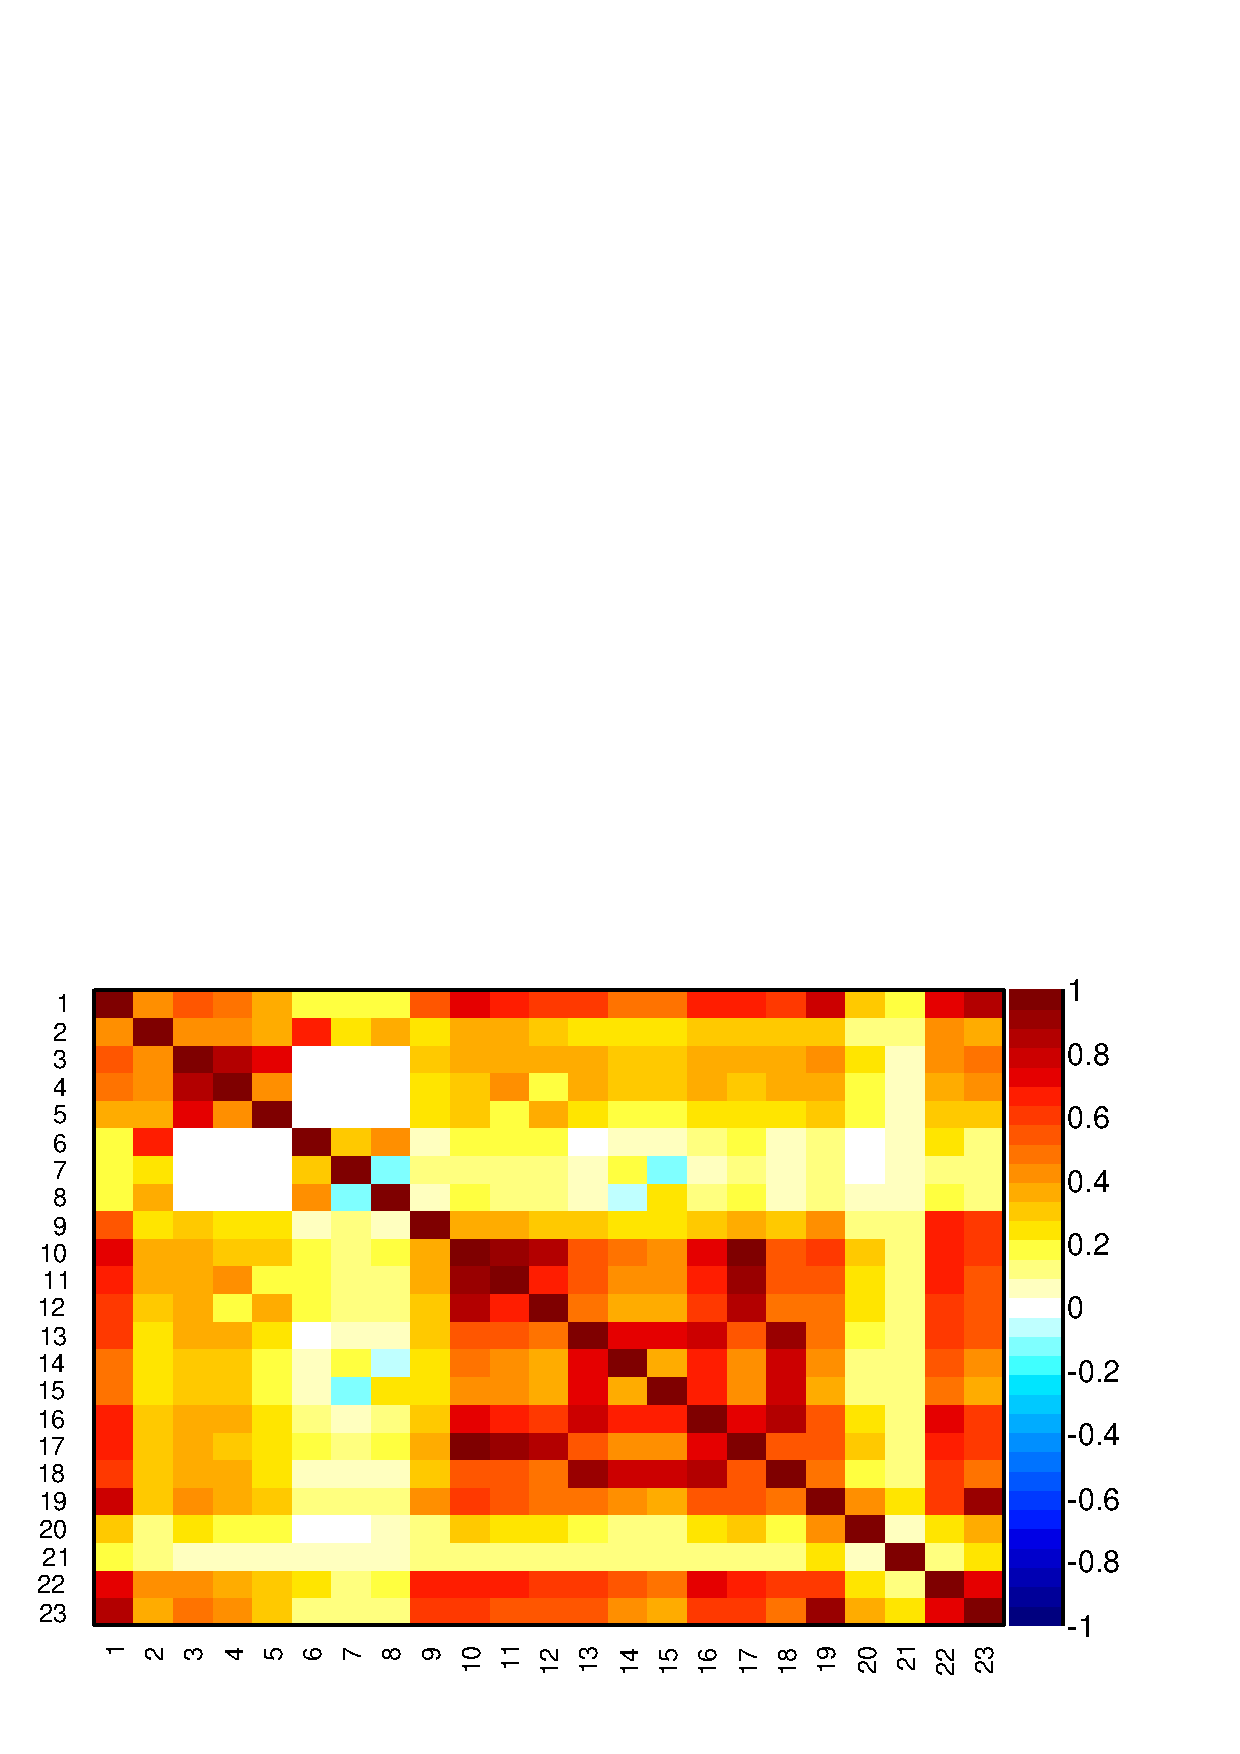
\includegraphics[width=0.8\textwidth]{Lmumu/figs/correlation.pdf}
\caption{Graphical representation of correlation matrix between truth and neural network inputs.
Column/row number 1 is correlation to the truth (whether candidate is signal or background). All
others give correlation between inputs with numbering scheme corresponding to the id column 
of Tab.~\ref{tab:Lb_nnInputs}. Correlation is calculated using all events without distinguishing signal and
background.}
\label{fig:Lb_nnCorrelation}
\end{figure}
%
\begin{figure}
\centering
\includegraphics[width=0.48\textwidth]{Lmumu/figs/TrainAndTest.pdf}
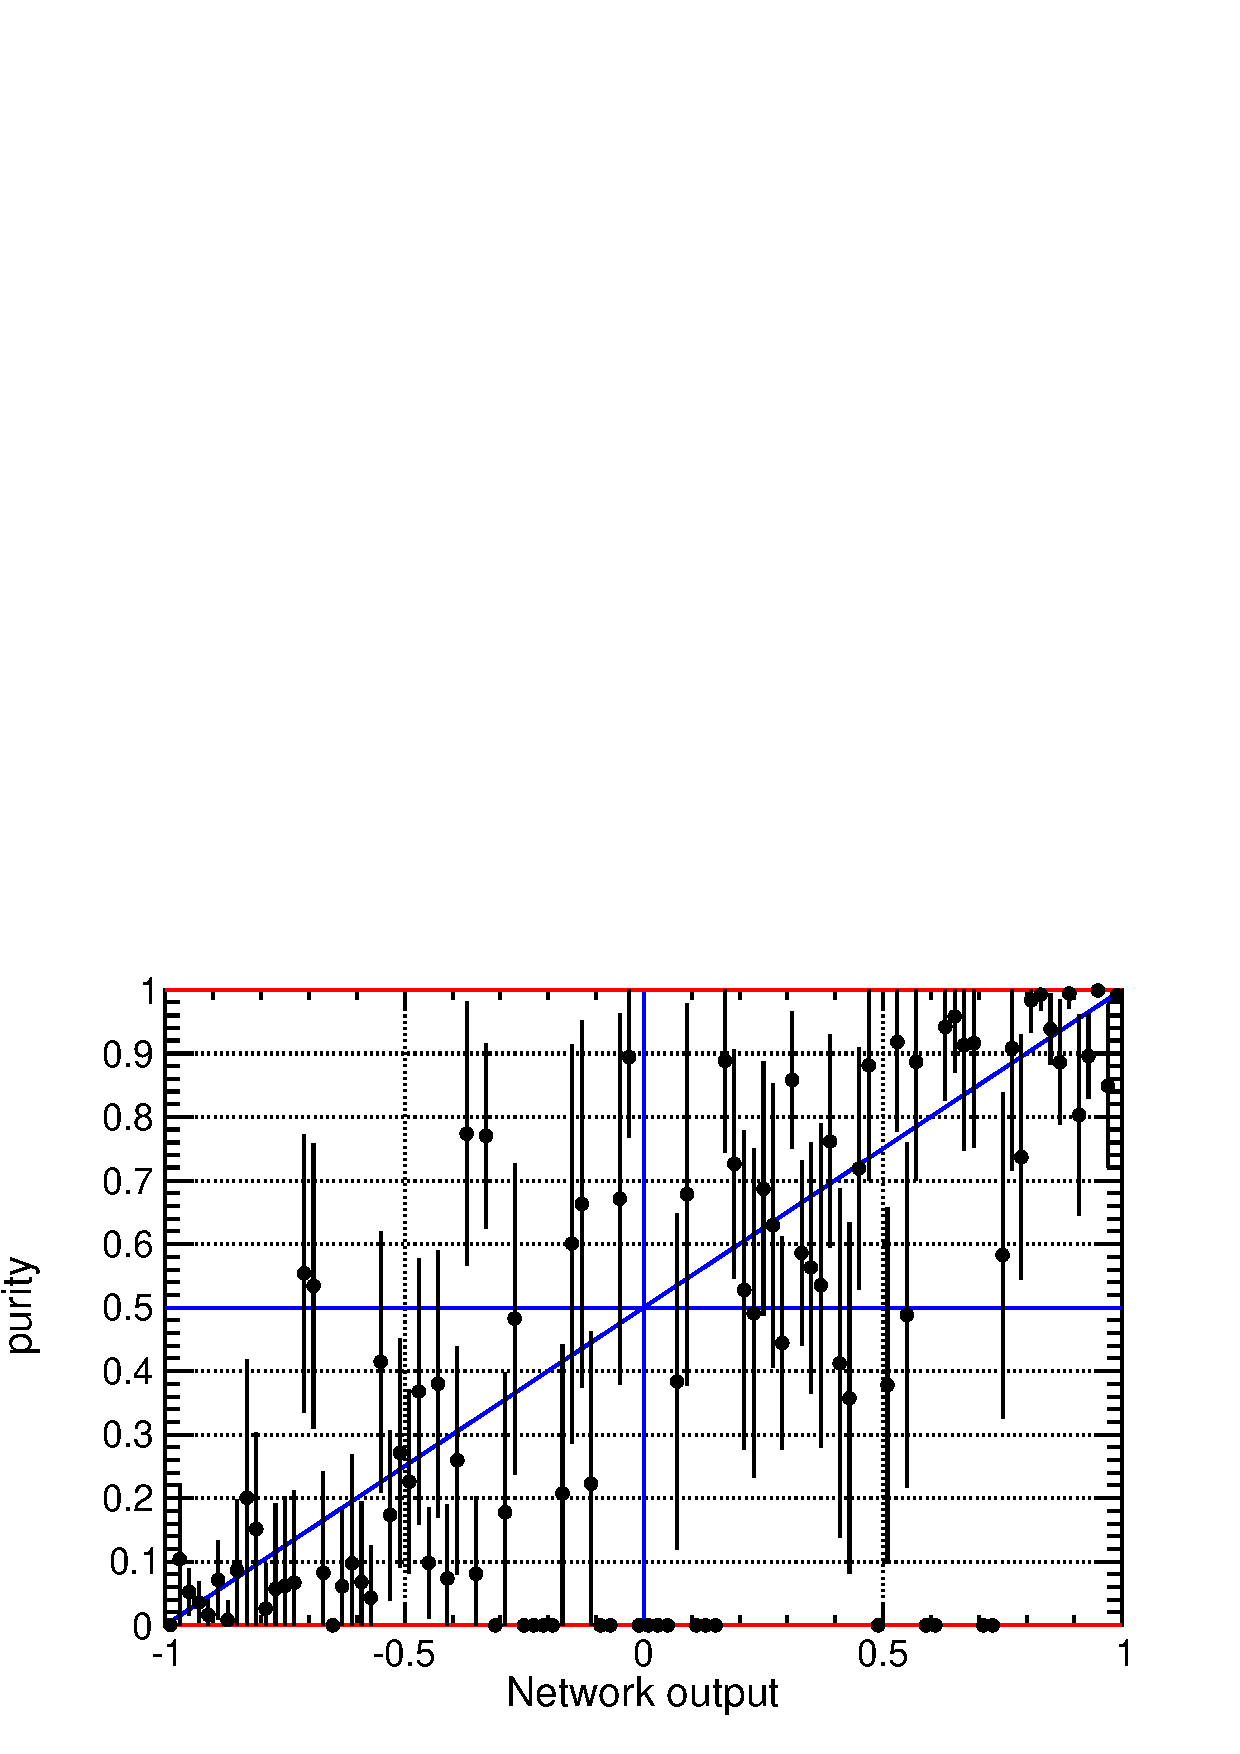
\includegraphics[width=0.48\textwidth]{Lmumu/figs/purity_NN.pdf}
\caption{(left) NN output distribution for training (points) and test (stripes) samples,
for signal and background events. (right) Purity as a function of neural network output.}
\label{fig:Lb_nnDist}
\end{figure}


It can happen that too much information is given to the classifier, which becomes able to 
calculate the invariant mass of the candidates from the input variables.
This can generate fake peaks and it is therefore important to check
for correlations between the 4-body invariant mass and the NN output.
Figure~\ref{fig:Lb_NNprofiles} reports the average NN output value as a function of
4-body $m(K\pi\mu\mu)$ invariant mass for data and simulation. The distributions
are flat indicating that no significant correlation is present.
%
\begin{figure}
\centering
\includegraphics[width=0.48\textwidth]{Lmumu/figs/NNout_profile_vs_LbMM_bkgData.pdf}
\includegraphics[width=0.48\textwidth]{Lmumu/figs/NNout_profile_vs_LbMM_MCsignal.pdf}
\caption{Average value of NN output as a function of \Lb mass for data sideband (left) and MC signal (right) events.}
\label{fig:Lb_NNprofiles}
\end{figure}




%As side note, we do not imply any particle identification on the \Lz daughters, nor we explicitly
%veto contributions where \KS is misreconstructed as \Lz. As will be seen later, \Bz decays
%containing \KS do not pose significant issues and any sensible attempt to significantly suppress
%them would result in significant loss of the statistics.




\section{MVA optimization}
\label{sec:Lb_mva_opt}

In the high \qsq region, where the signal is already observed, the final requirement on the neural network output
is chosen in order to maximise the significance, $N_{\mathrm{S}}/\sqrt{N_{\mathrm{S}}+N_{\mathrm{B}}}$, where
$N_\mathrm{S}$ is number of expected signal candidates and $N_\mathrm{B}$ the number of expected background candidates.
$N_\mathrm{S}$ is derived from simulation but, as an arbitrary number of events can be generated, it
needs to be normalised. To do this, the invariant mass distribution of real $\Lb\to\jpsi\Lz$ candidates
is fit after preselection (including all requirements but MVA). This is possible as the peak of the resonant
channel is already well visible after preselection. Then the resonant yield is scaled by the ratio
of between the $\Lb\to\Lz\mumu$ and $\Lb\to\jpsi\Lz$ branching fractions as measured 
by LHCb on 2011 data 
\begin{equation}
\BR(\Lb\to\Lz\mumu) / \BR(\Lb\to\jpsi\Lz) =  1.54 \times 10^{-3}
\end{equation}
\noindent
and $\jpsi\to\mumu$ branching fraction. In summary
\begin{equation}
N_\mathrm{S} = N_\jpsi \cdot \frac{\BR(\Lb\to\Lz\mumu)}{\BR(\Lb\to\jpsi\Lz) \cdot \BR(\jpsi\to\mumu) }.
\end{equation}
%
The number of expected backgrund events instead is derived fitting the data
sideband with an exponential and extrapolating under the singnal region.

In the low \qsq region, where the signal is unobserved, the so called ``Punzi figure of merit",
$N_{\mathrm{S}}/(n_\sigma/2+\sqrt{N_{\mathrm{B}}})$, is maximised \cite{Punzi:2003bu}.
This figure-of-merit is considered to be optimal for discovery and the parameter with $n_\sigma$ corresponds to
the number of expected standard deviations of significance, in this analysis $n_\sigma = 3$ is used.
Moreover the Punzi shape does not depend on the relative normalisation between signal and background, which
is important since the signal is still unobserved at low \qsq and existing predictions vary significantly
for this region. The dependence of the figure-of-merit for both \qsq regions are shown in Fig.~\ref{fig:Lb_FOM}, and curves
of signal efficiency versus background rejection are shown in Fig.~\ref{fig:Lb_ROC}.

For final selection the neural network output is required to be larger than 0.81 for high \qsq region
and 0.96 for the low \qsq one. Using these requirements the neural network retains approximately 96\% (66 \%)
of downstream candidates and 97 \% (82 \%) of long candidates for the selection at high (low) q2, with respect to
the preselected event sample. After the full selection $\sim 0.5$\% of the events contain multiple candidates
which are randomly rejected to keep only one candidate per event. 
%
%As reminder, in low \qsq region we start with much larger background than in high \qsq region.
%Moreover, while background rejection looks similar at selected requirement, in terms of amount of background kept, there is huge difference. 
%
To normalise the branching ratio measurement \jpsi events are selected using the low and high \qsq selection to normalise
respectively low and high \qsq intervals. 
%
\begin{figure}
\centering
\includegraphics[width=0.48\textwidth]{Lmumu/figs/significance_Lmumu_lowQ2.pdf}
\includegraphics[width=0.48\textwidth]{Lmumu/figs/significance_Lmumu_highQ2.pdf}
\caption{Dependence of figure-of-merit on the requirement on neural network output in the low \qsq
region (left) and high \qsq (right) regions. The vertical line corresponds to the chosen cut.}
\label{fig:Lb_FOM}
\end{figure}
%
\begin{figure}
\centering
\includegraphics[width=0.7\textwidth]{Lmumu/figs/ROC.pdf}
%\includegraphics[width=0.48\textwidth]{Lmumu/figs/ROC_Lmumu_highQ2.pdf}
\caption{Receiver operating characteristic (ROC) curves for low \qsq (black) and high \qsq (red).
They show the signal efficiency versus the background rejection.}
\label{fig:Lb_ROC}
\end{figure}

%\begin{figure}
%\centering
%\includegraphics[width=0.48\textwidth]{Lmumu/figs/Lb_MM_beforeMVAcut.pdf}
%\includegraphics[width=0.48\textwidth]{Lmumu/figs/Lb_MM_afterMVAcut.pdf}
%\caption{Invariant mass distribution $\Lb\to\Lz\mumu$ candidates before the MVA cut (left) and after the cut (right). This plot includes all data
%outside charmonium vetoes.}
%\label{fig:massDists}
%\end{figure}
%
%In Fig.~\ref{fig:massDists} we show invariant mass distributions of rare decay candidates before and after the MVA selection; the plot after MVA corresponds to final selection.
%In Fig.~\ref{fig:L0mass} we show the $m(p\pi)$ invariant mass of selected candidates, peaking at the PDG value for \Lz mass (1115 \mevcc).
%This indicates that our sample is dominated by real \Lz decays.  
%
%\begin{figure}
%\centering
%\includegraphics[width=0.7\textwidth]{Lmumu/figs/Lambda0_mass.pdf}
%\caption{Invariant mass $m(p\pi)$ of fully selected candidates.}
%\label{fig:L0mass}
%\end{figure}




\section{Trigger}

In addition specific trigger lines are selected, corresponding to events triggered by the muons
of the reconstructed candidate. This is denoted as Trigger On Signal (TOS).
The trigger lines used in the analysis are shown in Tab.~\ref{tab:Lb_triggerLines}.
The logical {\em or } of lines on the same lever is required and the logical {\em and }
and lined in different levels.
%
\begin{table}
\centering
\caption{Summary of trigger lines which candidates have to pass at various trigger levels.
Trigger is always required to be due to tracks of the candidate itself.}
\begin{tabular}{lc} \hline
Trigger Level &  Lines   \\ \hline
L0            & L0Muon  \\
                & L0DiMuon \\ \hline
Hlt1          & Hlt1TrackAllL0 \\ 
 %               & Hlt1DiMuonHighMass     \\
                & Hlt1TrackMuon      \\ \hline
Hlt2          & Hlt2Topo[2-4]BodyBBDT  \\
              & Hlt2TopoMu[2-4]BodyBBDT\\
              & Hlt2SingleMuon     \\
              & Hlt2DiMuonDetached \\ \hline
\end{tabular}
\label{tab:Lb_triggerLines}
\end{table}
%
The L0Muon trigger requires hits in the muon detector and triggers if a muon with $\pt > 1.5 \gevc$ is identified.
L0Dimuon imposes the same requirement on the sum of the transverse momenta of two tracks.
The Hlt1TrackAllL0 performs a partial reconstruction of the events and applied basic requirements on the
IP, $\chi^2$ and transverse momentum of tracks and triggers if the L0 decision is confirmed. Hlt1TrackMuon applies looser requirements 
but in addition requires the \verb!isMuon! variable (see Sec.~\ref{sec:PID_perf}) to be true to limit the yield.
Finally, at the Hlt2 level, a complete reconstruction is done and a multivariate analysis is used to identify decay structures. One of the main variables used at this stage is the distance of closest approach (DOCA), which is 
required to be less than 0.2 mm to form a 2-body object.
%
%Figure~\ref{fig:trigContrib} shows the single trigger efficiency, defined as if each line was alone.
%\begin{figure}
%\centering
%\includegraphics[width=0.48\textwidth]{Lmumu/figs/trig_highq2.pdf}
%\includegraphics[width=0.48\textwidth]{Lmumu/figs/trig_lowq2.pdf}
%\caption{ Single trigger efficiency for high \qsq events (left) and low \qsq (right). }
%\label{fig:trigContrib}
%\end{figure}


\section{Background from specific decays}

A survey of possible peaking backgrounds concluded that the only physics background
to take into account is coming from misreconstructed decays of \Bz to \KS with
two muons, whether via \jpsi or not. The lack of background from other decays is
mainly due to the particular topology of the \Lz decay which has a displaces vertex.
In order to study the effect of misreconstructed $\Bz\ra\jpsi\KS$ and $\Bz\ra\KS\mumu$ decays
simulated samples are used, where the \KS is reconstructed as a \Lz with a $p\rightarrow \pi$ identity
swap and $m(p\pi)$ in the \Lz mass window.
On data the $\Bz\ra\jpsi\KS$ contribution is clearly visible in the resonant channel mass distribution.
This background is not suppressed with specific cuts in this analysis as its mass shape is sufficiently distinct
the from \Lb signal, which allows to reliably model its contribution in the mass fits (see Sec.~\ref{sec:Lb_fit}).
For rare case a rough estimate of the size is made using the yield in the resonant channel
rescaled the measured ratios between the rare and resonant branching ratios.
Details are given in Sec.~\ref{sec:Lb_fit} and numbers of events predicted are reported in Tab.~\ref{tab:KSprediction}.
This contribution, although close to negligible is again considered in the fit.
A possible pollution due to $B^{+} \ra\mumu K^{*+}$ decays, where the $K^{*+}$
further decays into $\KS\pi$ is also investigated using a dedicated Monte Carlo sample and found to be negligible.
Finally, \Lb\ra\jpsi\Lz events radiating photons from the final state, can escape the \jpsi veto
and be reconstructed in the rare channel. Analysing simulated events it was found that the only
contribution is in the closest \qsq interval to the \jpsi tail, $6 < \qsq < 8$ \gevgevcccc.
In this interval 1.3\% of the \Lb\to\jpsi\Lz candidates are reconstructed but only 0.06\%
falls into the 4-body invariant mass window used for the fits. This corresponds to $\sim 6$
events, 4 of which in the downstream category. Given the low yield and that these events do
not peak under the signal but show a decaying distribution in the fit mass window this
background is considered as absorbed in the combinatorial background.
%Given that this contribution does not contribute in the region where we expect \Lb peak, we do
%not attempt to exclude this but it is again modelled in the fit.
In Fig.~\ref{fig:peakingBkgs} is reported the invariant mass distribution of simulated $\Lb\ra\jpsi\Lz$
events falling into the rare \qsq region.
%
\begin{figure}
\centering
\includegraphics[width=0.48\textwidth]{Lmumu/figs/Bu2Kstplus_mass.pdf}
\includegraphics[width=0.48\textwidth]{Lmumu/figs/JpsiL_leakage_mass.pdf}
\caption{ Invariant mass distributions of simulated $B^{+} \ra\mumu K^{*+}$ (left)
and \Lb\to\jpsi\Lz (right) candidates passing the full selection. Only \Lb\to\jpsi\Lz
candidates reconstructed in $\qsq < 8$ \gevgevcccc are selected.
Distributions are shown in the invariant mass range relevant for the analysis 
(see Sec.~\ref{sec:Lb_fit}). }
\label{fig:peakingBkgs}
\end{figure}


\section{Yield extraction}

Extended unbinned maximum likelihood fits are used to extract the yields of the rare and resonant channels.
The likelihood has the form:
%
\begin{equation}
\mathcal{L}=e^{-(N_\mathrm{S}+N_\mathrm{C}+N_{\mathrm{B}})}\times\prod_{i=1}^{N}\left[
N_\mathrm{S}P_{\mathrm{S}}(m_i)+N_\mathrm{C}P_\mathrm{C}(m_i)+N_{\mathrm{B}}P_{\mathrm{B}}(m_i)\right]
\end{equation}
\noindent
where $N_\mathrm{S}$, $N_\mathrm{C}$ and $N_\mathrm{B}$ are respectively the numbers of signal, 
combinatorial and \KS background events and the $P_i(m_i)$ are the corresponding probability density functions (PDF).
The fit variable is the 4-body $m(p\pi\mu\mu)$ invariant mass obtained from
a kinematical fit of the full decay chain in which each particle is constrained to point to its
assigned origin vertex and the invariant mass of the $p\pi$ system is constrained to be equal to
the world average for the \Lz baryon mass. In the resonant case a further constrain is used on the dimuon
mass to be equal to the known \jpsi mass. This method allows to improve the mass resolution giving
better defined peaks and therefore a more stable fit. For brevity, in the following these variables are
simply referred to as ``invariant mass".

\subsection{Fit description}
\label{sec:Lb_fit}

The fit is performed though the following steps:
%
\begin{itemize}
\item simulated distributions are fit to extract initial parameters;
\item the resonant data sample is fitted;
\item the rare sample is fitted fixing some parameters to those obtained in the previous cases.
\end{itemize}
%

In the first step simulated $\Lb\to\jpsi\Lz$ distributions are fitted using the signal PDF alone.
This is done separately for long and downstream candidates. Figure~\ref{fig:Lb_jpsiMCfit} shows 
distributions of candidates selected in the resonant sample with the fit function overlaid.
%
The signal is described as the sum of two Crystal Ball functions (CB) with
common mean ($m_0$) and tail slope ($n$). This is also known as Double Crystal Ball (DCB) function.
A single Crystal Ball~\cite{Skwarnicki:1986xj} is a probability
density function commonly used to model processes involving energy loss. In particular it is used
to describe resonances' peaks with radiative tails. This function 
consists of a Gaussian core and a power-law tail below a certain threshold and has form
%
\begin{equation}
C(x;\alpha,n,\bar{x},\sigma) = N \cdot
\begin{cases}
exp \left( -\frac{(x - \bar{x})^2}{2\sigma} \right)  & \mbox{   if   } \frac{(x - \bar{x})}{\sigma} > \alpha, \\
A\left( B - \frac{(x - \bar{x})}{\sigma} \right)^{-n} & \mbox{   if   } \frac{(x - \bar{x})}{\sigma} < \alpha,
\end{cases}
\end{equation}
%
where for normalisation and continuity
%
\begin{equation}
\label{CB}
\begin{array}{ll}
A = \left( \frac{c}{|\alpha|} \right))^n \cdot exp(- \frac{\alpha^2}{2}), \\
B = \frac{n}{|\alpha|} - |\alpha|.
\end{array}
\end{equation}
%
The full PDF for the resonant channel is therefore:
%
\begin{equation}
P_\mathrm{S}(m;m_0,\alpha_1,\alpha_2,f,n) = f \text{CB}(m;m_0,\sigma_1,\alpha_1,n)+(1-f)\text{CB}(m;m_0,\sigma_2,\alpha_2,n),
\end{equation}
%
where $f$ is the relative fraction of candidates falling into the first CB function.

\begin{figure}
\centering
\includegraphics[width=0.49\textwidth]{Lmumu/figs/MassFits/fitLb2JpsiL_DD_MC.pdf}
\includegraphics[width=0.49\textwidth]{Lmumu/figs/MassFits/fitLb2JpsiL_LL_MC.pdf}
\caption{Invariant mass distribution of $\Lb\ra\Lz\jpsi$ downstream (left) long (right) candidates.
The points show simulated data and the blue line is the signal fit function.}
\label{fig:Lb_jpsiMCfit}
\end{figure}

In a second step the fit to the resonant channel data sample is performed.
For this fit the tail slope parameter, ``$n$", which is highly correlated
with $\alpha_1$ and $\alpha_2$, is fixed to the value found in the fit to simulated data.
In this fit two background components are modelled: the combinatorial background,
parameterized with an exponential and the background from $\Bz\ra\jpsi\KS$ decays.
The shape used to describe the \KS background is obtained from a $\Bz\ra\jpsi\KS$ simulated
sample to which the full selection is applied. The invariant distribution of these events
is fit with a DCB function, which is then used to model the \KS background
in the $\Lb\to\jpsi\Lz$ fit. The fit to the simulated $\Bz\ra\jpsi\KS$ events
is reported in Fig.~\ref{fig:KSbkgFit}. When the \KS shape is introduced in the fit to the data all
its parameters are fixed. This is particularly important when fitting long candidates, where the \KS
peak is less evident, which does not allow to constrain many parameters. On the other hand, in order
to take into account possible data-simulation differences, an horizontal shift is added and left
floating (by adding a constant to the central value of the DCB, $m_0 \ra m_0 + m'$).
In summary, the free parameters in the fit to the resonant $\Lb\to\jpsi\Lz$ sample
are the yields of the signal and the combinatorial and \KS backgrounds, the slope
of the exponential and the horizontal shift of the \KS shape. Note that all parameters
of the fit to the long and downstream samples are independent.

\begin{figure}
\centering
\includegraphics[width=0.6\textwidth]{Lmumu/figs/MassFits/fitKS_bkg.pdf}
\caption{Invariant mass distribution of simulated $\Bz\ra\jpsi\KS$ events after 
full selection fitted a Double Crystal Ball function. }
\label{fig:KSbkgFit}
\end{figure}

Finally, the rare $\Lb\to\Lz\mumu$ data sample is fit. In this case the fit to the long
and downstream samples is performed simultaneously to obtain a more stable convergence. 
In this fit the signal is modelled with the same shape used in the resonant case as there is no physical
reason why they should be different. This method is also useful to limit systematic uncertainties
as the result will be given as a ratio between rare and resonant quantities.
However, the low statistics for the rare sample does not allow to constrain many parameters.
%,especially when dividing data in \qsq bins.
Therefore, all parameters of the signal shape are fixed to
the ones derived from the fit to the normalisation channel. However, to account for possible differences, 
arising from a different resolution in different \qsq regions, a scale factor is multiplied
to the widths of the two gaussian cores of the signal DCB: $\sigma_1 \rightarrow c\cdot \sigma_1$
and $\sigma_2 \rightarrow c\cdot \sigma_2$, where the two scale factors are the same. This factors
are fixed in the fit to data by fitting rare $\Lb\to\Lz\mumu$ simulated events in each \qsq bin and comparing
the widths with the ones found on the fit to the resonant simulated sample, namely
\begin{equation}
c = \sigma_{\mumu}^{MC} / \sigma_{\jpsi}^{MC}.
\end{equation}
Values obtained are $\sim 1.9$ for downstream candidates and $\sim 2.3$ for long candidates,
corresponding to the fact that in the resonant case a further constrain on the dimuon mass
is used, which improves the resolution by a factor of $\sim2$. The dependence of the scaling factor on \qsq 
is found to be small. For the fits on the long and downstream samples the parameters are always fixed to the
corresponding \jpsi fit; in this analysis shape parameters are never shared between the two candidate categories.

Also in the rare case the modelled background components are
the combinatorial background, described with an exponential function and the \KS background. 
The slope of the background is visibly different depending on the \qsq interval. This is partly due to the 
fact that at high \qsq the combinatorial changes slope because of a kinematical limit at low 4-body
masses imposed by the \qsq requirements. The exponential slopes are therefore left as independent
parameters in each \qsq interval. % and for the downstream and long samples.
The background component from $\Bz\to\KS\mumu$ decays is modelled using the same shapes used
for the resonant channel. However, in this case the horizontal shift is fixed to what found
for the resonant channel. The expected amount of misreconstructed $\Bz\ra\KS\mumu$
events is small and does not allow to determine reliably the yield. Therefore
this is fixed to the yield of $\Bz\ra\jpsi\KS$ decays rescaled by the expected ratio
of branching fractions between the resonant and rare channels. The \qsq distribution of $\Bz\ra\KS\mumu$ 
simulated events is used to predict the yield as a function of \qsq. Table~\ref{tab:KSprediction} reports the 
number of predicted $\Bz\ra\KS\mumu$ events in each \qsq interval obtained with the following formula:
\begin{equation}
N_{\KS\mumu}(\qsq) = N_{\jpsi\KS}\frac{B(\Bz\ra\KS\mumu)}{B(\Bz\ra\KS\jpsi)}\cdot \frac{1}{\epsilon_{rel}} \cdot B(\jpsi\ra\mumu) \frac{N(\qsq)_{MC}}{N^{tot}_{MC}} 
\end{equation}
where $N(\qsq)_{MC}$ is the number of simulated rare candidates falling in a \qsq interval after full selection and $N^{tot}_{MC}$ 
is the total number of simulated events. 
%The \KS\mumu contribution is then completely taken out to study systematic
%uncertainties as described in Sec.~\ref{sec:Lb_sys}.
%Only for the 6-8 \gevgevcccc bin, a background component coming from the residual of the \jpsi radiative tail is
%added, modelled using a the shape obtained studying simulated events and smoothed using the \verb!RooKeysPdf! method of \verb!RooFit!.
%This is then removed from the final fit becuase it returns zero yield.

\begin{table}
\centering
\caption{Predicted numbers of $\Bz\ra\KS\mumu$ events in each considered \qsq interval.}
\begin{tabular}{lcc} \hline 
 \qsq interval [\gevgevcccc]  & Downstream & Long \\ \hline
0.1--2.0 & 0.9 & 0.1 \\
2.0--4.0 & 0.9 & 0.1 \\
4.0--6.0 & 0.8 & 0.1 \\
6.0--8.0 & 1.1 & 0.1 \\
11.0--12.5 & 1.9 & 0.2 \\
15.0--16.0 & 1.1 & 0.1 \\
16.0--18.0 & 2.0 & 0.2 \\
18.0--20.0 & 1.1 & 0.1 \\ \hline
1.1--6.0 & 2.1 & 0.1 \\
15.0--20.0 & 4.2 & 0.5 \\ \hline
\end{tabular}
\label{tab:KSprediction}
\end{table}

As the fit on the rare sample is performed simultaneously on long and downstream candidates,
their two yields are not free to vary separately but are parameterised
as a function of the common branching fraction using the following formula:
%
\begin{equation}
N(\Lz\mumu)_{k}  = \left[ \frac{\mathrm{d}\mathcal{B}(\Lz\mumu)/\mathrm{d}\qsq}{\mathcal{B}(\jpsi\Lz)} \right]  \cdot
N(\jpsi\Lz)_{k} \cdot \varepsilon^{\mathrm{rel}}_{k} \cdot \frac {\Delta\qsq} { \mathcal{B}(\jpsi\to\mumu) },
\label{eq:relYield}
\end{equation}
%
where $k = $(LL,DD), $\Delta\qsq$ is the width of the \qsq interval and the only free parameter is the relative branching 
fraction ratio of the rare over \jpsi channels. For the branching fraction of the \jpsi\to\mumu decay the value 
reported in the PDG book, \mbox{$(5.93 \pm 0.06)\cdot 10^{-2}$~\cite{PDG2014}} is used and $\varepsilon^{rel}$ corresponds to
the relative efficiency between the rare and resonant channels obtained in Sec.~\ref{sec:Lb_eff}. 
In this formula the efficiencies and the normalisation yield appear as constants, namely 
$N(\Lz\mumu)_{k} = C_k \cdot \mathcal{B}^{rel}$. 
%These constants are then varied in order to obtain 
%systematic uncertainties on the final result as described in Sec.~\ref{sec:Lb_sys}.


\subsection{Fit results}



\begin{figure}
\centering
\includegraphics[width=0.75\textwidth]{Lmumu/figs/MassFits/Lb2JpsiL__DD_data.pdf}
\includegraphics[width=0.75\textwidth]{Lmumu/figs/MassFits/Lb2JpsiL__LL_data.pdf}
\includegraphics[width=0.49\textwidth]{Lmumu/figs/MassFits/Lb2JpsiL_DD_data_log_fitAndRes.pdf}
\includegraphics[width=0.49\textwidth]{Lmumu/figs/MassFits/Lb2JpsiL_LL_data_log_fitAndRes.pdf}
\caption{Invariant mass distributions of $\Lb\ra\jpsi\Lz$ downstream (top) and long (middle) candidates
selected with high \qsq requirements.
Bottom plots are the same as the upper ones but shown in logarithmic scale. Black points show data.
The blue solid line represents the total fit function, the black dashed line the signal, the red dashed line
the combinatorial background and the green dashed line the $\Bz\ra\KS\mumu$ background.}
\label{fig:Lb_totalFit}
\end{figure}
%
Figures~\ref{fig:Lb_totalFit} and~\ref{fig:Lb_totalFit_low} show fitted invariant mass distributions for
the normalisation channel, selected with the high \qsq and low \qsq requirements respectively.
%The $\chi^2$ value of the fit is $126$ for LL and $112$ for DD both with 140 degrees of freedom, which corresponds to probability of 80\% and 95\%.
Table~\ref{tab:Lb_rawYieldJpsi} reports the measured yields of $\Lb\ra\jpsi\Lz$ candidates found using the low 
and high \qsq selections. Values for the signal shape parameters are shown on Fig.~\ref{fig:Lb_totalFit}.
Fits to the rare $\Lb\ra\Lz\mumu$ samples are shown in Fig.~\ref{fig:Lb_Lmumu} for the integrated
$15 < \qsq < 20$ and $1.1 < \qsq < 6.0$~\gevgevcccc ~\qsq intervals, while
%The exponential slopes, the scale factors multiplied to the widths and the number of combinatorial events
%found from these fits are reported in Tab.~\ref{tab:Lb_rareParam}.
fitted invariant mass distribution in all other considered \qsq intervals are in Figs.~\ref{fig:Lb_differentialFitDD}
and~\ref{fig:Lb_differentialFitLL} for downstream and long candidates respectively.
The yields of rare candidates obtained from the fit are listed in Tab.~\ref{tab:Lb_rawYield} together with their significances.
Most candidates are found in the downstream sample, which comprises $\sim 80\,\%$ of the total yield.
Note that, since the fit is simultaneous to the two candidate categories, their yields
are not parameters free to float independently in the fit but are correlated via the branching ratio.
The statistical significance of the observed signal yields is evaluated as $\sqrt{2\Delta\ln{\mathcal{L}}}$, where
$\Delta\ln{\mathcal{L}}$ is the change in the logarithm of the likelihood function when the signal component
is excluded from the fit, relative to the nominal fit in which it is present.

\begin{table}
\centering
\caption{Number of \decay{\Lb}{\jpsi\Lz} candidates in the long and
  downstream categories found using the for low- and
  high-\qsq requirements. Uncertainties shown are statistical only.}
\begin{tabular}{lcc}
Selection & Long & Downstream					\\ \hline
high-\qsq	& $4313 \pm 70$	 	&  $11\,497 \pm 123$ \\
low-\qsq	& $3363 \pm 59$ 	&  $\phantom{0}\,7225 \pm 89\phantom{0}$  \\
 \hline
\end{tabular}
\label{tab:Lb_rawYieldJpsi}
\end{table}



\begin{table}
\centering
\caption{Signal yields ($N_\mathrm{S}$) obtained from the
  mass fit to \decay{\Lb}{\Lz\mumu} candidates in each \qsq interval
  together with their statistical significances. 
  The $8-11$ and $12.5-15$ \gevgevcccc ~\qsq intervals are excluded
  from the study as they are dominated by decays via charmonium resonances.}
\begin{tabular}{lcccc} \hline
 \qsq interval [\gevgevcccc] & DD & LL & Tot. yield & Significance \\ \hline
0.1 -- 2.0    &  $6.9 \pm 2.2$  &  $9.1 \pm 3.0$	 &  $16.0\pm5.3$            			 &  4.4 \\
2.0 -- 4.0    &  $1.8 \pm 1.7$  &  $3.0 \pm 2.8$ 	 &  $\phantom{0}4.8\pm4.7$  			 &  1.2 \\
4.0 -- 6.0    &  $0.4 \pm 0.9$  &  $0.6 \pm 1.4$	 &  $\phantom{0}0.9\pm2.3$  			 &  0.5 \\
6.0 -- 8.0    &  $4.3 \pm 2.0$   &  $7.2 \pm 3.3$	 &  $11.4\pm5.3$            			 &  2.7 \\
11.0 -- 12.5  &	 $14.6 \pm 2.9$  &  $42.8 \pm 8.5$   &  $\phantom{.0}60\pm12\phantom{.}$    &  6.5 \\
15.0 -- 16.0  &  $13.5 \pm 2.2$  &  $43.5 \pm 7.2$   &  $57\pm9$                			 &  8.7 \\
16.0 -- 18.0  &  $28.6 \pm 3.3$  &  $88.8 \pm 10.1$	 &  $118\pm13$              			 &  13  \\
18.0 -- 20.0  &  $22.4 \pm 2.6$  &  $78.0 \pm 8.9$	 &  $\phantom{.}100\pm11\phantom{.}$    &  14  \\
\hline
1.1 -- 6.0    &  $3.6 \pm 2.4$  &  $5.7 \pm 3.8$	 &  $\phantom{0}9.4\pm6.3$  			&  1.7 \\
15.0 -- 20.0  &  $64.6 \pm 4.7$  &  $209.6 \pm 15.3$ &  $276\pm20$              			&  21  \\
\end{tabular}
\label{tab:Lb_rawYield}
\end{table}

\begin{figure}
\centering
\includegraphics[width=0.49\textwidth]{Lmumu/figs/MassFits/Lb2JpsiL__lowSel_DD_data.pdf}
\includegraphics[width=0.49\textwidth]{Lmumu/figs/MassFits/Lb2JpsiL__lowSel_LL_data.pdf}
\caption{Invariant mass distribution of $\Lb\ra\jpsi\Lz$ for downstream (left) and long (right) candidates
 selected with low \qsq requirements.}
\label{fig:Lb_totalFit_low}
\end{figure}
%
%
\begin{figure}
\centering
\includegraphics[width=0.7\textwidth]{Lmumu/figs/paper/figure13.pdf}
\includegraphics[width=0.7\textwidth]{Lmumu/figs/paper/figure2.pdf}
\caption{Invariant mass distributions of $\Lb\ra\Lz\mumu$ candidates in the integrated 0.1--6.0 \gevgevcccc(top)
and 15--20 \gevgevcccc (bottom) ~\qsq intervals. Points show data combining downstream and long candidates together.
The blue solid line represents the total fit function and the dashed red line the combinatorial background.}
%\includegraphics[width=0.54\textwidth]{Lmumu/figs/MassFits/Lb2Lmumu_DD_lowQ2_fitAndRes.pdf}
%\includegraphics[width=0.54\textwidth]{Lmumu/figs/MassFits/Lb2Lmumu_LL_lowQ2_fitAndRes.pdf}
%\includegraphics[width=0.54\textwidth]{Lmumu/figs/MassFits/Lb2Lmumu_DD_highQ2_fitAndRes.pdf}
%\includegraphics[width=0.54\textwidth]{Lmumu/figs/MassFits/Lb2Lmumu_LL_highQ2_fitAndRes.pdf}
%\caption{Invariant mass distribution of $\Lb\ra\Lz\mumu$ candidates in the integrated 0.1--6.0 (top)
%\gevgevcccc ~\qsq interval for downstream (left) and long (right) candidates. The points show data, the blue line
%and 15.0--20.0 (bottom) \gevgevcccc \qsq intervals.
%The blue solid line represents the total fit function and the dashed red line the combinatorial background.}
\label{fig:Lb_Lmumu}
\end{figure}
%
\begin{figure}
\centering
\includegraphics[width=1.\textwidth]{Lmumu/figs/MassFits/q2_fits_DD_plot2.pdf}
\includegraphics[width=1.\textwidth]{Lmumu/figs/MassFits/q2_fits_DD_plot1.pdf}
\caption{Invariant mass distributions of rare $\Lb\ra\Lz\mumu$ candidates in the considered \qsq bins
 %[0.1,2], [2,4], [4,6], [6,8], [11,12.5], [15,16], [16,18], [18,20]
 for downstream candidates. }
\label{fig:Lb_differentialFitDD}
\end{figure}

\begin{figure}
\centering
\includegraphics[width=1.\textwidth]{Lmumu/figs/MassFits/q2_fits_LL_plot2.pdf}
\includegraphics[width=1.\textwidth]{Lmumu/figs/MassFits/q2_fits_LL_plot1.pdf}
\caption{Invariant mass distributions of rare $\Lb\ra\Lz\mumu$ candidates in the considered \qsq bins
 %[0.1,2], [2,4], [4,6], [6,8], [11,12.5], [15,16], [16,18], [18,20]
 for long candidates. }
\label{fig:Lb_differentialFitLL}
\end{figure}



%\begin{table}
%\centering
%\caption{Values of exponential slope, $b$, and scale factors, $c$ found from the fit
%to the resonant data sample and fixed from the fit to the rare data sample.}
%\begin{tabular}{|c|c|c|}
%\hline
%Parameter  			 & Downstream & Long	\\ 
%\hline
%\multicolumn{3}{|c|}{ 15.0--20.0 \gevgevcccc}  \\
%\hline

%$b$ 				& $0.0006 \pm 0.0003$		 		& 	$0.0012 \pm 0.0008$        \\
%$c$ 				& $1.9027 \pm 0.0001$ 				&	$2.2910 \pm 0.0001$        \\
%%$N_{exp}$ 			& $393^{+23}_{-22}$	&	 $64^{+9}_{-8}$       \\

%\hline
%\multicolumn{3}{|c|}{ 1.1--6.0 \gevgevcccc}  \\

%\hline
%$b$ 				& $-0.0026 \pm 0.0004$				&	$-0.0036 \pm 0.0011$	 \\
%$c$ 				& $1.9208 \pm 0.0001$				&	$2.3504 \pm 0.0001$        \\
%%$N_{exp}$ 			& $203^{+15}_{-14}$	&	$34^{+7}_{-6}$       \\
%\hline

%\end{tabular}
%\label{tab:Lb_rareParam}
%\end{table}




\clearpage


\section{Efficiency}
\label{sec:Lb_eff}

The selection efficiency is calculated for each decay according to the formula
\begin{equation}
\varepsilon^{tot}=\varepsilon(Geom)\varepsilon(Det|Geom)\varepsilon(Reco|Det)\varepsilon(MVA|Reco)\varepsilon(Trig|MVA).
\end{equation}
In this expression the first term gives the efficiency to have final state particles in the LHCb acceptance.
The second term handles the possibility of \Lz escaping the detector or interacting with it and therefore
never decaying into $p\pi$; this term is referred to as ``detection" efficiency.
The third term carries information about the reconstruction and pre-selection efficiencies,
which are kept together given that boundaries between them are completely artificial.
The fourth part deals with the efficiency of the neural network candidates that passed the pre--selection. 
Finally, the last term handles the trigger efficiency for candidates which are accepted by the full selection.
%Trigger efficiency is calculated before the MVA one because the training is performed on untriggered data to save statistics.
Most of the efficiency components are evaluated using the simulated samples described in Sec.~\ref{sec:Lb_simulation}.
Only the efficiency of the PID requirement for the proton (see Tab.~\ref{tab:Lb_stripping}) is separately derived
with a data--driven method because the simulation does not provide a good description of PID variables. 
%For complete information, all absolute efficiencies for the two decays $\Lb\to\Lz\mumu$ and $\Lb\to\jpsi\Lz$ are
%separately listed in the next subsections. 
Representative absolute efficiencies' values are given in the next sections.
However, for the analysis itself only the relative efficiency,
$\varepsilon($\Lb\to\Lz\mumu$)/\varepsilon(\Lb\to\jpsi\Lz)$, is used. 


\subsection{Geometric acceptance}
\label{sec:Lb_geomAcc}
In order to save disk space and time the simulation only includes events in which the final muons
are in the detector acceptance and therefore can be reconstructed. This corresponds to a requirement for each
of the muons to be in an interval \mbox{$10 < \theta < 400$~mrad}, where $\theta$ is the angle between
the muon momentum and the beam line. The efficiency of this requirement is obtained by using 
a separate simulated sample, where events are generated in the full space.
The geometric efficiency varies between 18\% at high-\qsq and 20\% at low-\qsq;
Fig.~\ref{fig:Lb_absEff} shows the dependence of this efficiency as a function of \qsq.

%In Tab.~\ref{tab:Lb_geom_eff} the efficiencies due to the geometrical acceptance are listed
%in bins of \qsq for $\Lb\to\Lz\mumu$ decays.
%
%\begin{table}[h]
%\centering
%\caption{Absolute geometrical acceptance in the two integrated \qsq bins
%derived from generator level simulated samples. Uncertainties are statistical only.}
%\begin{tabular}{$l^c}
%\rowstyle{\bfseries}
%\boldmath{\qsq} [\boldmath{\gevgevcccc}]     & \boldmath{$\varepsilon(Geom)$}   \\ \hline
%0.1--2.0 		&  $0.2359 \pm 0.0008$  \\
%2.0--4.0 		&  $0.2098 \pm 0.0007$  \\
%4.0--6.0 		&  $0.2008 \pm 0.0007$  \\
%6.0--8.0 		&  $0.1960 \pm 0.0008$  \\
%9.1--10.1 	&  $0.1927 \pm 0.0012$  \\
%11.0--12.5 	&  $0.1897 \pm 0.0010$  \\
%15.0--16.0 	&  $0.1896 \pm 0.0015$  \\
%16.0--18.0 	&  $0.1872 \pm 0.0012$  \\
%18.0--20.0 	&  $0.1870 \pm 0.0016$  \\
%\hline
%\phantom{x}1.1 -- 6.0\phantom{x} 	&  $0.2072 \pm 0.0005$  \\
%15.0 -- 20.0 	&  $0.1876 \pm 0.0008$  \\
%\end{tabular}
%\label{tab:Lb_geom_eff}
%\end{table}


\subsection{Reconstruction and neural network efficiencies}

The efficiency to reconstruct the decays together with the pre-selection requirements is
evaluated from simulated data. 
%For the evaluation we use the most recent LHCb measurement of \Lb
%lifetime of $1.482\pm0.03$ ps\cite{LHCb--PAPER--2013--032} and \Lb polarisation $0.06\pm0.09$ \cite{Aaij:2013oxa}.
%Table~\ref{tab:Lb_recoEff} reports values of reconstruction efficiency for the two integrated \qsq intervals
 %for long and downstream candidates.
The reconstruction efficiency is subdivided in ``Detection" and ``Reconstruction and pre-selection" efficiencies.
In fact, since \Lz is a long lived particle, there is a non-negligible probability that it interacts in the detector
or escapes from it and therefore never decays in proton and pion. 
%The efficiency for this to happen is what is called ``Detection" efficiency. 
The reconstruction efficiency includes the probability 
for the tracks to produce observable signatures and to pass the pre-selection 
requirements. This component does not include the efficiency
of the PID cut that appears in Tab.~\ref{tab:Lb_stripping}, which is kept separate
because PID variables are not well described by the simulation.
The detection efficiency varies between 88\% at low-\qsq and 92\% at high-\qsq
while the reconstruction efficiency is almost flat in \qsq at 6.6\% for downstream candidates
and 2.0\% for long candidates.
%Fig.~\ref{fig:Lb_absEff} shows the dependence of these efficiencies as a function of \qsq.
% and therefore a data-driven method is used instead (see Sec.~\ref{sec:PIDeff}).
%
%
%\begin{table}[h]
%\centering
%\caption{Absolute detection and reconstruction plus stripping efficiencies.
%Reconstruction efficiency is given separately for downstream and long candidates. Uncertainties are statistical only. }
%\begin{tabular}{$l^c^c^c}
%\rowstyle{\bfseries}
%\boldmath{\qsq} [\boldmath{\gevgevcccc}] & \boldmath{$\varepsilon(Det)$} & \boldmath{$\varepsilon(Reco)^{\rm DD}$} & \boldmath{$\varepsilon(Reco)^{\rm LL}$} \\ \hline
%0.1--2.0 		&  $0.8793 \pm 0.0005$	&  $0.0519 \pm 0.0006$	&  $0.0194 \pm 0.0004$  \\
%2.0--4.0 		&  $0.8850 \pm 0.0004$	&  $0.0664 \pm 0.0006$	&  $0.0195 \pm 0.0004$  \\
%4.0--6.0 		&  $0.8902 \pm 0.0004$	&  $0.0717 \pm 0.0007$	&  $0.0209 \pm 0.0004$  \\
%6.0--8.0 		&  $0.8962 \pm 0.0005$	&  $0.0756 \pm 0.0007$	&  $0.0212 \pm 0.0004$  \\
%9.1--10.1 	&  $0.9022 \pm 0.0007$	&  $0.0787 \pm 0.0011$	&  $0.0220 \pm 0.0006$  \\
%11.0--12.5 	&  $0.9084 \pm 0.0006$	&  $0.0799 \pm 0.0009$	&  $0.0221 \pm 0.0005$  \\
%15.0--16.0 	&  $0.9187 \pm 0.0009$	&  $0.0736 \pm 0.0012$	&  $0.0179 \pm 0.0007$  \\
%16.0--18.0 	&  $0.9247 \pm 0.0007$	&  $0.0696 \pm 0.0010$	&  $0.0169 \pm 0.0005$  \\
%18.0--20.0 	&  $0.9318 \pm 0.0009$	&  $0.0600 \pm 0.0011$	&  $0.0136 \pm 0.0006$  \\
%\hline
%\phantom{x}1.1 -- 6.0\phantom{x} 	&  $0.8868 \pm 0.0003$	&  $0.0684 \pm 0.00041$	&  $0.0202 \pm 0.0002$  \\
%15.0 -- 20.0 	&  $0.9260 \pm 0.0005$	&  $0.0669 \pm 0.00063$	&  $0.0159 \pm 0.0003$  \\
%\end{tabular}
%\label{tab:Lb_recoEff}
%\end{table}
%
%\subsubsection{Neural Networks efficiency}
%
The MVA selection efficiency is again evaluated from simulated samples
and it is observed to vary from 55\% to 88\% for downstream candidates
and from 74\% to 96\% for long candidates.
Fig.~\ref{fig:Lb_absEff} shows the dependence of these efficiencies as a function of \qsq.
%Results are shown in 
%Tab.~\ref{tab:Lb_mvaEff} for the two integrated \qsq intervals.
The sudden jump in MVA efficiency at $\sim 9$~\gevcc~is due to the fact that
a different figure-of-merit is used to optimise the MVA requirement in the low- and high-\qsq regions,
which results in different efficiencies.
%
%\begin{table}[h]
%\centering
%\caption{Neural network selection efficiency. Uncertainties are statistical only.}
%\begin{tabular}{$l^c^c}
%\rowstyle{\bfseries}
%\boldmath{\qsq} [\boldmath{\gevgevcccc}] & \boldmath{$\varepsilon(MVA)^{\rm DD}$} & \boldmath{$\varepsilon(MVA)^{\rm LL}$}\\ \hline
%0.1--2.0 		&  $0.623 \pm 0.008$	&  $0.813 \pm 0.011$  \\
%2.0--4.0 		&  $0.583 \pm 0.007$	&  $0.757 \pm 0.011$  \\
%4.0--6.0 		&  $0.584 \pm 0.007$	&  $0.776 \pm 0.011$  \\
%6.0--8.0 		&  $0.588 \pm 0.007$	&  $0.778 \pm 0.011$  \\
%9.1--10.1 	&  $0.904 \pm 0.006$	&  $0.948 \pm 0.008$  \\
%11.0--12.5 	&  $0.888 \pm 0.005$	&  $0.944 \pm 0.007$  \\
%15.0--16.0 	&  $0.882 \pm 0.007$	&  $0.929 \pm 0.012$  \\
%16.0--18.0 	&  $0.847 \pm 0.007$	&  $0.928 \pm 0.009$  \\
%18.0--20.0 	&  $0.831 \pm 0.009$	&  $0.889 \pm 0.016$  \\
%\hline
%\phantom{x}1.1 -- 6.0\phantom{x} 	&  $0.584 \pm 0.005$	&  $0.772 \pm 0.007$  \\
%15.0 -- 20.0 	&  $0.849 \pm 0.005$	&  $0.917 \pm 0.007$  \\
%\end{tabular}
%\label{tab:Lb_mvaEff}
%\end{table}

%This efficiency component was crosschecked using \jpsi real data. In these events the peak is well visible even before
%the MVA cut. Therefore it is possible to fit the peak to subtract the background and then do the same procedure after the MVA cut.
%Counting events in an interval of 20 $MeV/c^2$ around the \jpsi invariant mass and (5605,5635) in \Lb invariant mass
%we obtain the following efficiencies: 86.1\% for DD events and 93.1\% for LL.
%Given the uncertainty on the background subtraction prodecure we quintify the uncertainty on this procedure
%in $\sim 4\%$ by varing mass windows and look at the change in the efficiency obtained. The pure statistical error
%on these values is 0.7\%. Therefore comparing numbers in table \ref{tab:jpsiEff}, obtained using \jpsi\Lz MC, we find them compatible within 1 sigma.   



\subsection{Trigger efficiency}
\label{sec:Lb_trigger_eff}

The trigger efficiency is again evaluated using a simulated sample. It increases with \qsq and varies 
from $\sim 57\%$ to $\sim 86\%$ for both downstream and long candidates.
Fig.~\ref{fig:Lb_absEff} shows the dependence of this efficiency as a function of \qsq.
Using the high statistics resonant channel it is possible to crosscheck using data the trigger efficiency obtained using the simulation.
In LHCb triggered events can fall into two categories: events triggered by a track which is part of a signal candidate, 
Trigger On Signal (TOS), or by other tracks in the event, Trigger Independent of Signal (TIS). 
As the TIS and TOS categories are not exclusive the TIS sample provides a control
sample which can be used to obtain the efficiency for TOS trigger. This can be calculated with the formula:
\begin{equation}
\varepsilon_{\rm TOS} = \frac{\text{TIS  and TOS }}{\text{TIS}}.
\end{equation}
As data contains background the numbers of signal candidates in the ``TIS" and \mbox{``TIS and TOS"}
categories are not just determined by counting but from fits to the 4-body invariant mass, 
$m(p\pi\mu\mu)$, distributions after applying these requirements. This procedure takes the name of TISTOS method. 
Using the data--driven method an efficiency of ($70 \pm 5$)\% is obtained, while this is calculated to be
($73.33 \pm 0.02$)\% using the simulation. Results are therefore compatible within $1\sigma$. 
%
%\begin{table}[h]
%\centering
%\caption{Absolute trigger efficiencies for selected events as determined
%from the simulation separately for downstream and long events.}
%\begin{tabular}{$l^c^c} 
%\rowstyle{\bfseries}
%\boldmath{\qsq} [\boldmath{\gevgevcccc}] & \boldmath{$\varepsilon(Trig)^{\rm DD}$} & \boldmath{$\varepsilon(Trig)^{\rm LL}$}\\ \hline

%0.1--2.0 	&  $0.560 \pm 0.008$	&  $0.577 \pm 0.012$  \\
%2.0--4.0 	&  $0.606 \pm 0.006$	&  $0.651 \pm 0.010$  \\
%4.0--6.0 	&  $0.623 \pm 0.006$	&  $0.674 \pm 0.010$  \\
%6.0--8.0 	&  $0.669 \pm 0.006$	&  $0.706 \pm 0.010$  \\
%9.1--10.1 	&  $0.700 \pm 0.007$	&  $0.722 \pm 0.013$  \\
%11.0--12.5 	&  $0.744 \pm 0.006$	&  $0.738 \pm 0.011$  \\
%15.0--16.0 	&  $0.818 \pm 0.008$	&  $0.826 \pm 0.015$  \\
%16.0--18.0 	&  $0.836 \pm 0.006$	&  $0.860 \pm 0.011$  \\
%18.0--20.0 	&  $0.857 \pm 0.008$	&  $0.863 \pm 0.015$  \\
%\hline
%\phantom{x}1.1 -- 6.0\phantom{x} 	&  $0.610 \pm 0.004$	&  $0.653 \pm 0.007$  \\
%15.0 -- 20.0 	&  $0.839 \pm 0.004$	&  $0.853 \pm 0.008$  \\
%\end{tabular}
%\label{tab:Lb_triggerEfficiency}
%\end{table}


\subsection{PID efficiency}
\label{sec:PIDeff}
For long tracks a PID requirement on protons (\verb!PID!p$ > -5$) is applied. The simulation is known not to
describe PID variables well and therefore a data-driven method is used to obtain this efficiency component.
This is done using the \verb!PIDCalib! package (see Sec.~\ref{sec:PID_calib}), which uses as calibration samples
decays where particles can be identified due to their kinematic properties. In the case of protons a sample of
\Lz particles is used, where the proton can be identified because it always has the highest momentum.
The package allows to divide the phase space in bins of variables relevant for PID
performances; in this analysis momentum and pseudorapidity are used.
Using the calibration sample the efficiency is derived in each two-dimensional bin.
Finally, to take into account that the decay channel under study could have different kinematical distributions
than the calibration sample these efficiency tables are used to re-weight the simulation.
The PID efficiency varies from 97.3\% at low-\qsq to 98.2\% at high-\qsq. 
%Absolute PID efficiencies are listed in Tab.~\ref{tab:Lb_PIDabs} for the two integrated \qsq intervals.
%
%\begin{table}[h]
%\centering
%\caption{Absolute PID efficiencies in \qsq bins.}
%\begin{tabular}{$l^c}
%\rowstyle{\bfseries}
%\boldmath{\qsq} [\boldmath{\gevgevcccc}]	&      \boldmath{$\varepsilon(PID)$}  \\  \hline
%0.1--2.0     &  $97.32 \pm 0.012$   \\
%2.0--4.0     &  $97.42 \pm 0.012$   \\
%4.0--6.0     &  $97.59 \pm 0.011$   \\
%6.0--8.0     &  $97.70 \pm 0.010$   \\
%11.0--12.5   &  $98.04 \pm 0.009$   \\
%15.0--16.0   &  $98.31 \pm 0.006$   \\
%16.0--18.0   &  $98.10 \pm 0.005$   \\
%18.0--20.0   &  $98.11 \pm 0.001$  \\
%\hline
%\phantom{x}1.1 -- 6.0\phantom{x}     &  $97.49 \pm 0.007$   \\
%15.0 -- 20.0   &  $98.17 \pm 0.003$  \\
%\jpsi       &  $97.89 \pm 0.005$   \\
%\end{tabular}
%\label{tab:Lb_PIDabs}
%\end{table}



\subsection{Relative efficiencies}

In the previous sections absolute efficiencies values were given for the rare channel, which are summarised in Fig.~\ref{fig:Lb_absEff}.
This section reports the corresponding relative efficiencies with respect to the $\Lb\to\jpsi\Lz$ channel, which will be
used to correct the yields and obtain the differential branching fraction. Table~\ref{tab:jpsiEff} reports the absolute 
efficiency values for the \jpsi channel used to derive the relative efficiencies.
Relative geometric, detection and PID efficiencies are listed in Tab.~\ref{tab:relativeGeometric}, while
Tabs.~\ref{tab:allRelativeEffDD} and \ref{tab:allRelativeEffLL} report relative reconstruction, trigger and MVA efficiencies 
separately for downstream and long candidates. Since the latter three components are obtained from the 
same simulated sample their statistical uncertainties are correlated. Therefore, the total of the three is also reported 
as a single efficiency and labeled ``Full Selection". Finally, Tab.~\ref{tab:Lb_effSummary} reports the total of 
all relative efficiencies, which will be then used to correct the raw yields and calculate the differential branching fraction.
Uncertainties reflect the statistics of both rare and resonant samples, while systematic uncertainties are discussed in following sections.

\begin{table}
\centering
\caption{Absolute efficiency values for $\Lb\to\jpsi\Lz$; uncertainties are statistical only.}
\begin{tabular}{$l^c^c}
\rowstyle{\bfseries}
Efficiency				& 	Downstream				& 	Long				\\  \hline		
$\varepsilon(Geom)$ 	&   	\multicolumn{2}{c}{	$0.1818 \pm 0.0003$ } 	\\	
$\varepsilon(Det)$ 		&   	\multicolumn{2}{c}{	$0.9017 \pm 0.0003$ } 	\\
$\varepsilon(Reco)$	 	& 	$0.0724 \pm 0.0004$   & $0.0203 \pm 0.0002$     \\
$\varepsilon(PID)$		&	--	&  $97.89 \pm 0.005$   \\
$\varepsilon(MVA)$ 		&	$0.882 \pm 0.002$   & $0.942 \pm 0.002$     \\
$\varepsilon(Trig)$ 		&	$0.697 \pm 0.003$   & $0.734 \pm 0.005$     \\ \hline
Full Selection			&	$0.0445 \pm 0.0003$   & $0.0140 \pm 0.0002$     \\ \hline
Total  				&	$0.00729 \pm 0.00005$   & $0.00230 \pm 0.00003$    	\\
\end{tabular}
\label{tab:jpsiEff}
\end{table}


\begin{table}
\centering
\caption{Relative geometric, detection and PID relative efficiencies between
$\Lb\to\Lz\mumu$ and $\Lb\to\jpsi\Lz$ decays; uncertainties reflect the statistics of both samples.}
\begin{tabular}{$l^c^c^c}
\rowstyle{\bfseries}
\boldmath{\qsq} [\boldmath{\gevgevcccc}] & Geometric & Detection & PID \\ \hline
%0.1--2.0 		&  $1.2976 \pm 0.0050$ 	&  $0.9751 \pm 0.0006$  \\
%2.0--4.0 		&  $1.1541 \pm 0.0043$ 	&  $0.9814 \pm 0.0005$  \\
%4.0--6.0 		&  $1.1043 \pm 0.0044$ 	&  $0.9872 \pm 0.0006$  \\
%6.0--8.0 		&  $1.0778 \pm 0.0045$ 	&  $0.9939 \pm 0.0006$  \\
%9.1--10.1 	&  $1.0596 \pm 0.0065$ 	&  $1.0005 \pm 0.0008$  \\
%11.0--12.5 	&  $1.0431 \pm 0.0058$ 	&  $1.0074 \pm 0.0007$  \\
%15.0--16.0 	&  $1.0426 \pm 0.0084$ 	&  $1.0188 \pm 0.0010$  \\
%16.0--18.0 	&  $1.0296 \pm 0.0068$ 	&  $1.0255 \pm 0.0008$  \\
%18.0--20.0 	&  $1.0288 \pm 0.0087$ 	&  $1.0333 \pm 0.0010$  \\
%\hline
%1.1 -- 6.0 	&  $1.1396 \pm 0.0031$ 	&  $0.9835 \pm 0.0004$  \\
%15.0 -- 20.0 	&  $1.0320 \pm 0.0048$ 	&  $1.0269 \pm 0.0006$  \\

\phantom{x}0.1 -- 2.0\phantom{x} 		&  $1.2976 \pm 0.0050$ 	&  $0.9751 \pm 0.0006$  & $0.99418 \pm 0.00013$ \\
\phantom{x}2.0 -- 4.0\phantom{x} 		&  $1.1541 \pm 0.0043$ 	&  $0.9814 \pm 0.0005$  & $0.99523 \pm 0.00013$ \\
\phantom{x}4.0 -- 6.0\phantom{x} 		&  $1.1043 \pm 0.0044$ 	&  $0.9872 \pm 0.0006$  & $0.99699 \pm 0.00012$  \\
\phantom{x}6.0 -- 8.0\phantom{x} 		&  $1.0778 \pm 0.0045$ 	&  $0.9939 \pm 0.0006$  & $0.99805 \pm 0.00011$ \\
11.0 -- 12.5 	&  $1.0431 \pm 0.0058$ 	&  $1.0074 \pm 0.0007$  & $1.00151 \pm 0.00010$ \\
15.0 -- 16.0 	&  $1.0426 \pm 0.0084$ 	&  $1.0188 \pm 0.0010$  & $1.00431 \pm 0.00008$ \\
16.0 -- 18.0 	&  $1.0296 \pm 0.0068$ 	&  $1.0255 \pm 0.0008$  & $1.00215 \pm 0.00008$ \\
18.0 -- 20.0 	&  $1.0288 \pm 0.0087$ 	&  $1.0333 \pm 0.0010$  & $1.00226 \pm 0.00005$ \\
\hline
\phantom{x}1.1 -- 6.0\phantom{x} 		&  $1.1396 \pm 0.0031$ 	&  $0.9835 \pm 0.0004$  & $0.99589 \pm 0.00009$ \\
15.0 -- 20.0 	&  $1.0320 \pm 0.0048$ 	&  $1.0269 \pm 0.0006$  & $1.00281 \pm 0.00006$ \\

\end{tabular}
\label{tab:relativeGeometric}
\end{table}



\begin{table}
\centering
\caption{Relative efficiencies between $\Lb\to\Lz\mumu$ and $\Lb\to\jpsi\Lz$ decays for downstream 
candidates; uncertainties reflect the statistics of both samples.}
\begin{tabular}{$l^c^c^c^c^c^c}
\rowstyle{\bfseries}
\boldmath{\qsq} [\boldmath{\gevgevcccc}]      & Reconstruction         & MVA                 & Trigger       & Full Selection      \\
\hline
\phantom{x}0.1 -- 2.0\phantom{x} 		&  $0.721 \pm 0.009$ 	&  $0.706 \pm 0.010$ 	&  $0.805 \pm 0.011$ 	&  $0.410 \pm 0.009$  \\
\phantom{x}2.0 -- 4.0\phantom{x} 		&  $0.920 \pm 0.010$ 	&  $0.661 \pm 0.008$ 	&  $0.870 \pm 0.010$ 	&  $0.529 \pm 0.010$  \\
\phantom{x}4.0 -- 6.0\phantom{x} 		&  $0.997 \pm 0.010$ 	&  $0.662 \pm 0.008$ 	&  $0.895 \pm 0.010$ 	&  $0.590 \pm 0.011$  \\
\phantom{x}6.0 -- 8.0\phantom{x} 		&  $1.050 \pm 0.011$ 	&  $0.665 \pm 0.008$ 	&  $0.960 \pm 0.010$ 	&  $0.671 \pm 0.012$  \\
%9.1--10.1 	&  $1.092 \pm 0.015$ 	&  $1.025 \pm 0.007$ 	&  $1.005 \pm 0.011$ 	&  $1.125 \pm 0.021$  \\
11.0 -- 12.5 	&  $1.112 \pm 0.014$ 	&  $1.007 \pm 0.006$ 	&  $1.069 \pm 0.009$ 	&  $1.197 \pm 0.019$  \\
15.0 -- 16.0 	&  $1.019 \pm 0.018$ 	&  $1.000 \pm 0.009$ 	&  $1.175 \pm 0.012$ 	&  $1.197 \pm 0.026$  \\
16.0 -- 18.0 	&  $0.968 \pm 0.014$ 	&  $0.961 \pm 0.008$ 	&  $1.200 \pm 0.010$ 	&  $1.115 \pm 0.020$  \\
18.0 -- 20.0 	&  $0.832 \pm 0.016$ 	&  $0.943 \pm 0.010$ 	&  $1.231 \pm 0.012$ 	&  $0.966 \pm 0.023$  \\
\hline
\phantom{x}1.1 -- 6.0\phantom{x} 	&  $0.950 \pm 0.007$ 	&  $0.663 \pm 0.005$ 	&  $0.876 \pm 0.007$ 	&  $0.551 \pm 0.007$  \\
15.0 -- 20.0 	&  $0.929 \pm 0.010$ 	&  $0.963 \pm 0.005$ 	&  $1.204 \pm 0.007$ 	&  $1.077 \pm 0.014$  \\

\end{tabular}
\label{tab:allRelativeEffDD}
\end{table}

\begin{table}
\centering
\caption{Relative efficiencies between $\Lb\to\Lz\mumu$ and $\Lb\to\jpsi\Lz$ decays for 
long candidates; uncertainties reflect the statistics of both samples.}
\begin{tabular}{$l^c^c^c^c^c} 
\rowstyle{\bfseries}
\boldmath{\qsq} [\boldmath{\gevgevcccc}]      & Recoscruction          & MVA                 & Trigger         & Full Selection \\
\hline
\phantom{x}0.1 -- 2.0\phantom{x} 		&  $0.96 \pm 0.02$ 	&  $0.863 \pm 0.012$ 	&  $0.79 \pm 0.02$ 	&  $0.65 \pm 0.02$  \\
\phantom{x}2.0 -- 4.0\phantom{x} 		&  $0.97 \pm 0.02$ 	&  $0.803 \pm 0.012$ 	&  $0.89 \pm 0.02$ 	&  $0.69 \pm 0.02$  \\
\phantom{x}4.0 -- 6.0\phantom{x} 		&  $1.04 \pm 0.02$ 	&  $0.824 \pm 0.012$ 	&  $0.92 \pm 0.02$ 	&  $0.79 \pm 0.02$  \\
\phantom{x}6.0 -- 8.0\phantom{x} 		&  $1.05 \pm 0.02$ 	&  $0.825 \pm 0.012$ 	&  $0.96 \pm 0.02$ 	&  $0.84 \pm 0.02$  \\
%9.1--10.1 	&  $1.08 \pm 0.03$ 	&  $1.007 \pm 0.009$ 	&  $0.98 \pm 0.02$ 	&  $1.07 \pm 0.04$  \\
11.0 -- 12.5 	&  $1.10 \pm 0.03$ 	&  $1.002 \pm 0.008$ 	&  $1.01 \pm 0.02$ 	&  $1.10 \pm 0.03$  \\
15.0 -- 16.0 	&  $0.89 \pm 0.03$ 	&  $0.987 \pm 0.013$ 	&  $1.13 \pm 0.02$ 	&  $0.98 \pm 0.04$  \\
16.0 -- 18.0 	&  $0.84 \pm 0.03$ 	&  $0.985 \pm 0.010$ 	&  $1.17 \pm 0.02$ 	&  $0.97 \pm 0.03$  \\
18.0 -- 20.0 	&  $0.67 \pm 0.03$ 	&  $0.944 \pm 0.017$ 	&  $1.18 \pm 0.02$ 	&  $0.75 \pm 0.04$  \\
\hline
\phantom{x}1.1 -- 6.0\phantom{x} 	&  $1.00 \pm 0.02$ 	&  $0.820 \pm 0.008$ 	&  $0.89 \pm 0.01$ 	&  $0.73 \pm 0.02$  \\
15.0 -- 20.0 	&  $0.78 \pm 0.02$ 	&  $0.973 \pm 0.008$ 	&  $1.16 \pm 0.01$ 	&  $0.89 \pm 0.02$  \\

\end{tabular}
\label{tab:allRelativeEffLL}
\end{table}

%\begin{table}
%\centering
%\caption{Relative PID efficiencies in \qsq bins}
%\begin{tabular}{lc} \hline
%\qsq [\gevgevcccc]	&     Rel.  PID eff.            \\  \hline
%0.1--2.0    & $0.99418 \pm 0.00013$  \\
%2.0--4.0    & $0.99523 \pm 0.00013$   \\
%4.0--6.0    & $0.99699 \pm 0.00012$   \\
%6.0--8.0    & $0.99805 \pm 0.00011$   \\
%11.0--12.5  & $1.00151 \pm 0.00010$   \\
%15.0--16.0  & $1.00431 \pm 0.00008$   \\
%16.0--18.0  & $1.00215 \pm 0.00008$   \\
%18.0--20.0  & $1.00226 \pm 0.00005$   \\
%\hline
%1.1 -- 6.0    & $0.99589 \pm 0.00009$   \\
%15.0 -- 20.0  & $1.00281 \pm 0.00006$  \\
%\hline
%\end{tabular}
%\label{tab:Lb_PIDrel}
%\end{table}



%\begin{table}
%\centering
%\begin{tabular}{lcc} \hline\hline
%\qsq bin & Tot. rel. eff. DD &  Tot. rel. eff. LL \\ \hline

%0.1--2.0 	&  $0.51821 \pm 0.01208$	&  $0.82385 \pm 0.02846$  \\
%2.0--4.0 	&  $0.59863 \pm 0.01200$	&  $0.78194 \pm 0.02444$  \\
%4.0--6.0 	&  $0.64365 \pm 0.01253$	&  $0.85667 \pm 0.02594$  \\
%6.0--8.0 	&  $0.71846 \pm 0.01360$	&  $0.89726 \pm 0.02670$  \\
%9.1--10.1 	&  $1.19267 \pm 0.02374$	&  $1.13929 \pm 0.04046$  \\
%11.0--12.5 	&  $1.25735 \pm 0.02163$	&  $1.15949 \pm 0.03701$  \\
%15.0--16.0 	&  $1.27185 \pm 0.02971$	&  $1.04571 \pm 0.04716$  \\
%16.0--18.0 	&  $1.17743 \pm 0.02295$	&  $1.01962 \pm 0.03663$  \\
%18.0--20.0 	&  $1.02651 \pm 0.02607$	&  $0.79500 \pm 0.03937$  \\
%\hline
%1.1 -- 6.0 	&  $0.61800 \pm 0.00855$	&  $0.81966 \pm 0.01804$  \\
%15.0 -- 20.0 	&  $1.14181 \pm 0.01622$	&  $0.94460 \pm 0.02518$  \\

%\hline
%\end{tabular}
%\caption{Total relative efficiency between $\Lb\to\Lz\mumu$ and $\Lb\to\jpsi\Lz$ decays. For downstream events and long events.}
%\label{tab:totalRelativeEff}
%\end{table}
	

\begin{figure}
\centering
\includegraphics[width=0.48\textwidth]{Lmumu/figs/efficiencies/BR/effvsq2_DD_geom.pdf}
\includegraphics[width=0.48\textwidth]{Lmumu/figs/efficiencies/BR/effvsq2_DD_det.pdf}
\includegraphics[width=0.48\textwidth]{Lmumu/figs/efficiencies/BR/effvsq2_DD_reco.pdf}
\includegraphics[width=0.48\textwidth]{Lmumu/figs/efficiencies/BR/effvsq2_LL_reco.pdf}
\includegraphics[width=0.48\textwidth]{Lmumu/figs/efficiencies/BR/effvsq2_DD_mva.pdf}
\includegraphics[width=0.48\textwidth]{Lmumu/figs/efficiencies/BR/effvsq2_LL_mva.pdf}
\includegraphics[width=0.48\textwidth]{Lmumu/figs/efficiencies/BR/effvsq2_DD_trig.pdf}
\includegraphics[width=0.48\textwidth]{Lmumu/figs/efficiencies/BR/effvsq2_LL_trig.pdf}
\caption{Absolute efficiencies as a function of \qsq: geometric efficiency (a), 
detection efficiency (b), reconstruction efficiency for DD (c) and LL (d) candidates, 
MVA efficiency for DD (e) and LL (f) and trigger efficiency for DD (g) and LL (h).}
\label{fig:Lb_absEff}
\end{figure}

\clearpage

\section{Systematic uncertainties}
\label{sec:Lb_sys}

This section describes the main sources of systematic uncertainty considered.

\subsection{Systematic uncertainty on the yields}
\label{sec:Lb_yield_sys}

The choice of specific PDFs to model the invariant mass distributions could result
in a bias. The first step in assessing the potential systematic effect due to the signal PDF choice is fitting 
 the $\Lb\to\jpsi\Lz$ data sample using a number of models in order to understand which ones provide a plausible 
 description of data. Table~\ref{PDFsys} reports the $\chisq$ and corresponding p-values obtained using different
models including: the default model (a DCB function), a simple Gaussian function,
a single Crystal Ball function and the sum of two Gaussians (Double Gaussian, DG). The only two models that
give a reasonable p-value are the (default) DCB and the DG functions.
In a second step, simulated pseudo-experiments are generated and fit with the two chosen models.
Events are generated according to a density function given by the default model with parameters taken
from the fit to data, separately for each \qsq interval. In this way, for each \qsq interval, a specific
shape is reproduced including a data-like background level and slope. Furthermore, a number 
of events comparable to that found in data is generated. For each pseudo-experiment a normalised
bias is calculated as
%
\begin{equation}
b = \left(\frac{N^{DCB}_{\ell\ell}}{N^{DCB}_{\jpsi}} - \frac{N^{DG}_{\ell\ell}}{N^{DG}_{\jpsi}}\right) / \frac{N^{DCB}_{\ell\ell}}{N^{DCB}_{\jpsi}},
\end{equation}
%
where $N^{model}_{\ell\ell}$ and $N^{model}_{\jpsi}$ are the numbers of rare and resonant candidates
observed using a specific model. %The distribution of biases have approximately gaussian shape.
The average bias over 1000 pseudo-experiments is taken
as the systematic uncertainty. Note that in each case the rare and normalisation channels are fit
with the same signal model and, while for the default case the rare parameters are fixed to those found
for the resonant channel, they are left free to vary in the second model in order to assess
a possible systematic effect due to the constraints on the parameters in the same study.

\begin{center}
\begin{table}[h]
\centering
\caption{$\chisq$, \text{ndf}, p-values and number of signal events obtained fitting \mbox{$\Lb\to\jpsi\Lz$} data using different models.}
\begin{tabular}{$l^c^c^c^c}
\rowstyle{\bfseries}
Model   		& \boldmath{$\chisq/\text{ndf}$}  & \boldmath{\text{ndf}}  & p-value  & \boldmath{$N_{evts}$} \\ \hline
%\multicolumn{4}{c}{Rare channel} \\
%DCB  (default)  &    1.1   &   47   &    0.34       &  279.8  \\
%Gauss 		&    1.0   &   46   &    0.55       &  270.3  \\
%Double gauss  	&    1.0   &   44   &    0.47       &  270.3  \\
%CB  		&    1.0   &   44   &    0.47       &  270.4  \\
%\hline
%$K_S$ removed 	&    1.0   &   47   &    0.41       &  283.5  \\
%\hline
%\multicolumn{4}{c}{$J/\psi$ channel} \\
%\hline
DCB  (default)	&    1.0   &   187   &    0.51      & 9965.4  \\
Gauss			&    1.8   &   193   &    $\sim 0$  & 9615.7 \\
Double Gauss  	&    1.1   &   191   &    0.45      & 9882.4  \\
CB  			&    1.5   &   191   &    $\sim 0$  & 9802.4 \\
%\hline
%Fixed $K_S$ shape &  1.6   &   188   &    $\sim 0$  & 9976.3  \\
%With $K^{*0}$ bkg &    1.0   &   188   &    0.53      & 9976.4  \\
\end{tabular}
\label{PDFsys}
\end{table}
\end{center}

For the background PDF systematic, the rare channel is re-fit but the yield of the \KS component is allowed to vary freely, 
in contrast to the default fit where it is fixed to the yield predicted by the simulation. The same procedure as applied to the signal PDF case, 
using pseudo-experiments to evaluate the mean bias due to the choice of PDF, is also followed here. Results are reported in Tab.~\ref{tab:pdfsys}. 
%The most affected \qsq interval is the one in the middle of the charmonium
%resonances, where a combination of lower statistics and higher background leaves more freedom to the signal shape.
Finally, a background component for $B^{+} \ra K^{*+}(\KS\pi^+)\mumu$ decays is added to the fit, modelled using
the distribution of simulated candidates after full selection. No significant bias is found for this component.

\begin{center}
\begin{table}[h]
\centering
\begin{tabular}{$l^c^c^c}
\rowstyle{\bfseries}
\boldmath{\qsq [\gevgevcccc]} & Signal PDF (\%)  & Background PDF (\%)  & Total  (\%) \\ \hline
\phantom{x}0.1 -- 2.0\phantom{x}       &    3.2   &  1.1   &    3.4    \\
\phantom{x}2.0 -- 4.0\phantom{x}       &    2.9   &  2.4   &    3.8    \\
\phantom{x}4.0 -- 6.0\phantom{x}       &    4.6   &  4.8   &    6.6    \\
\phantom{x}6.0 -- 8.0\phantom{x}       &    1.2   &  1.7   &    2.0    \\

11.0 -- 12.5		&    2.6   &  1.8   &    3.2	\\
15.0 -- 16.0 	&    1.3   &  2.5   &    2.8	\\
16.0 -- 18.0 	&    0.6   &  1.3   &    1.4	\\
18.0 -- 20.0 	&    1.7   &  1.8   &    2.5	\\

\hline
\phantom{x}1.1 -- 6.0\phantom{x}       &    0.1   &  4.2   &    4.2    \\
15.0 -- 20.0		&    1.0   &  0.2   &    1.1	\\
\end{tabular}
\caption{Values of systematic uncertainties due to the choice of signal and background shapes in bins of \qsq. }
\label{tab:pdfsys}
\end{table}
\end{center}




\subsection{Systematic uncertainties on the efficiency determination}

%As we study \qsq dependence of the differential branching fraction, one of the challenges is to properly account for
%correlations. There are three types of correlations we need to handle, one is correlation between
%normalisation and signal decay, second is correlation between different \qsq bins and finally as we
%split efficiency into three parts (geometry, selection and trigger), we should take also correlation
%amongst them into account. The last class of correlations is in principle rather easy to treat, but
%fully correct treatment of the first two classes would require to split the systematic uncertainties
%to correlated amongst \qsq bins and uncorrelated part, which given our statistics would complicate
%the presentation of the result. For simplicity we treat correlations where systematic uncertainty is
%significant and neglect correlations amongst \qsq bins when uncertainty for given source is small
%compared to dominant sources.
%
Systematic uncertainties on the efficiency determination are due to the limited knowledge
of the decay properties such as the \Lb lifetime and production polarisation.
The systematic uncertainties are directly evaluated on the relative efficiencies as these are the ones that
are actually used in the analysis. It should be noted that not all sources contribute to each part
of the efficiency. For brevity, this section only reports estimates of the systematic
uncertainties obtained, while the full information is contained in Appendix~\ref{app:Lb_systematics_app}.
%Numerical values of systematic uncertainties on relative efficiencies are in
%table \ref{tab:relativeGeomSys} and for \ref{tab:relativeDetSys} for geometrical and detection efficiency;
%\ref{tab:relativeRecoSys}, \ref{tab:relativeTrigSys} and \ref{tab:relativeMVAsys} for reconstruction, trigger and neural
%networks for long-long and down-down events.
%Finally, we remind the reader that we always use fully simulated phase space sample we weight those, modelling
%polarisation and decay structure. The MC sample used is always the same thus within the single decay there is always
%correlation in our simulated events.
%

\subsubsection{Effect of new physics on the decay model}
\label{sec:WCvariation}

New physics could affect the decay model used to simulate events by adding contributions to the $C_7$ and $C_9$ 
Wilson coefficients. This would result in a modification of the simulated \qsq spectra and therefore of the efficiency obtained 
from simulation. To assess this systematic the Wilson coefficients are modified by adding a new physics component
($C_i \rightarrow C_i + C_i^{ \rm NP}$). 
\begin{figure}[hb]
\centering
\includegraphics[width=0.8\textwidth]{Lmumu/figs/wilson_q2.pdf}
\caption{The \qsq spectrum of $\Lb\to\Lz\mumu$ simulated events weighted with models embedding different sets of Wilson coefficients.
The black distribution corresponds to the weights used to calculate nominal efficiencies.}
\label{fig:wilson_q2}
\end{figure}
Figure~\ref{fig:wilson_q2} shows \qsq spectra
obtained by weighting the simulation for a model embedding the default and three modified sets
of Wilson coefficients. The values used, reported on the plot legend, are inspired
to maintain compatibility with the recent LHCb measurement of the $P'_5$ observable~\cite{Descotes-Genon:2013wba}.
The biggest effect is observed in the very low \qsq region, below 2~\gevgevcccc, where the efficiency can change
by up to 7\%, while it changes 3 -- 4\% between 3 and 4~\gevgevcccc~and 2 -- 3\% in the rest of the spectrum.
As this analysis is performed under the hypothesis that the decays are described by the SM,
these values are given for completeness but are not added 
as systematic uncertainties. 

%\begin{figure}
%\centering
%\includegraphics[width=0.48\textwidth]{Lmumu/figs/rel_wilson1_sysAll.pdf}
%\includegraphics[width=0.48\textwidth]{Lmumu/figs/rel_wilson2_sysAll.pdf} \\
%\includegraphics[width=0.48\textwidth]{Lmumu/figs/rel_wilson3_sysAll.pdf}
%\caption{Relative effect of different Wilson Coefficients sets on the total efficiency in bins of \qsq.}
%\label{fig:wilson_diff}
%\end{figure}

\subsubsection{Simulation statistics}

The limited statistics of the simulated samples used to determine the efficiencies is considered 
as a source of systematic uncertainty.
While it is not the dominant source, its size is not completely negligible, 
therefore, when reporting efficiency values, the statistical uncertainty due to the  
rare and resonant channels is always considered. 
%While it would be useful to treat part from normalisation channel separately due to the correlation 
%across \qsq bins, given its size we decide to suppress it as in final presentation its effect is hard to see.

\subsubsection{Production polarisation and decay structure}
\label{sec:BRpolsys}

One of the main unknowns that affects the determination of the efficiencies, is the angular structure of
the decays and the related production polarisation, which is a parameter of the model.
%The normalisation decay $\Lb\to\jpsi\Lz$ is also re-weighted and $\Lb\to\Lz\mumu$ is
%distributed according to the model described in appendix \ref{ap:LbLmumuAngular}.
%
To assess the systematic uncertainty due to the knowledge of the production polarisation for $\Lb\to\Lz\mumu$ decays
the polarisation parameter in the model is varied by one standard deviation from the central value of the
most recent LHCb measurement, $P_b = 0.06 \pm 0.09$~\cite{Aaij:2013oxa}. The full observed difference is
taken as systematic uncertainty. To assess the systematic uncertainty due to the decay structure,
an alternative set of form factors is used based on lattice QCD calculations~\cite{Detmold:2012vy}. 
The two models are compared and the full difference is taken as systematic uncertainty.
%
In total this results in an uncertainty of \mbox{$\sim1.3\%$} for long candidates and \mbox{$\sim0.6\%$} for downstream
candidates, mostly coming from the knowledge of the production polarisation.

\subsubsection{\Lb lifetime}

The \Lb lifetime is known with limited precision. For the evaluation of efficiencies the
world average value, $1.482\pm0.030$~ps$^{-1}$~\cite{Aaij:2013oha}, is used. This is
varied by one standard deviation from the measured value to assess the systematic uncertainty.
Only the case where both signal and normalisation channels are varied in the same direction are considered.
The largest difference from the default lifetime case is taken as the systematic uncertainty,
which is found to vary from $\sim 0.4\%$ at low-\qsq to $\sim 0.1\%$ at high-\qsq.
%We do not attempt to separate out part correlated amongst \qsq bins. This source does not affect
%geometric acceptance, which is defined purely by requirements on angles of each muon with respect to
%beam axis.

\subsubsection{Downstream candidates reconstruction efficiency}

%In the LHCb detector, \Lz can be reconstructed using long or downstream tracks. The distinction is mainly
%driven by the geometry of the detector. A potential issue is that fraction of \Lz reconstructed
%from long tracks and downstream tracks does not fully agree with simulation. For $\Lb\to\jpsi\Lz$
%decay we determine on data that $(26.44 \pm 0.70)$\% of \Lz candidates are reconstructed from long tracks.
%On contrary in simulation of the same decay, only $21.15\pm0.24$\% of candidates are reconstructed
%from long tracks. The same ratio on phase space simulation of $\Lb\to\Lz\mumu$ is $21.54\pm0.14$\%
%(integrated over \qsq). From this we conclude that this ratio is expected to be similar in the two samples and
%that simulation does not fully match data.

Other analysis in LHCb using particles reconstructed from downstream tracks showed that
the efficiency for these candidates is not perfectly simulated.
For example, Fig.~\ref{KS_vtxeff} shows the ratio between the reconstruction efficiency for downstream candidates
in data and simulation found analysing \KS events~\cite{Blake:1631348}. This effect is not
yet fully understood and is currently under study. It seems to be mainly due to a poor simulation
of the vertexing efficiency for downstream tracks.
%
%
However, as the analysis is performed separately for downstream and long candidates and efficiencies are calculated separately, 
the effect of this mis-modelling, present in both the rare and resonant channels, largely cancels in their ratio.
Nevertheless, a systematic uncertainty is assessed by re-weighting simulated candidates 
by the efficiency ratio between data and simulation found for \KS as a function of its momentum (see Fig.~\ref{KS_vtxeff}). 
The efficiencies obtained using the weighted and unweighted simulation are compared and the full difference is taken as the systematic uncertainty. 
As the discrepancy shows little dependence on momentum, dependencies due to the different momentum 
distributions of \Lz and \KS are assumed to be negligible. This results in a systematic uncertainty for downstream candidates
of $\sim 0.4\%$ at low-\qsq and $\sim 1.2\%$ at high-\qsq.

\begin{figure}
\centering
\includegraphics[width=0.8\textwidth]{Lmumu/figs/DDvtx_eff_POwen.pdf}
\caption{Ratio of reconstruction efficiency in data and simulation found using \KS events~\cite{Blake:1631348}.}
\label{KS_vtxeff}
\end{figure}

\subsubsection{Data-simulation discrepancies}

The simulation used to calculate the efficiencies is weighted to 
improve its description of data as described in Sec.~\ref{sec:kinWeight}.
The influence of this procedure on the efficiency determination is checked by comparing values obtained with
and without re-weighting. The effect is negligible with respect to other systematics considered.
%After the kinematical re-weighting there could still be some data-simulation discrepancies.
%In particular the PID variables, used in the Neural Networks, are not perfectly described in the MC.
%We checked if this could be a source of systematics by comparing sideband subtracted data Monte Carlo re-weighted for the
%\Lb kinematics and extracting a further weight to match the PID variable.
%Figure \ref{fig:PIDmysys} shows the difference between the efficiency calculated with and without the further PID weight.
%In all \qsq bins the difference is always compativle with zero within one sigma and therefore we do not add any further systematic
%due to the PIDmu variable modelling.

%\begin{figure}
%\centering
%\includegraphics[width=0.6\textwidth]{Lmumu/figs/PIDmu_sys.pdf}
%\caption{Difference between the efficiency calculated with and without the weight to match the PIDmu distributions
%in data and MC as a function of \qsq.}
%\label{fig:PIDmysys}
%\end{figure}


\section{Differential branching fraction extraction}
\label{sec:Lb_BRsummary}

In this section the differential branching fraction of the $\Lb\to\Lz\mumu$ decay is calculated 
relative to the $\Lb\ra\jpsi\Lz$ channel as a function of \qsq.
The values are directly obtained from the fit to the rare sample by parameterising
the downstream and long yields with the following formula:
%
\begin{equation}
N(\Lz\mumu)_{k}  = \left[ \frac{\mathrm{d}\mathcal{B}(\Lz\mumu)/\mathrm{d}\qsq}{\mathcal{B}(\jpsi\Lz)} \right]  \cdot
N(\jpsi\Lz)_{k} \cdot \varepsilon^{\mathrm{rel}}_{k} \cdot \frac {\Delta\qsq} { \mathcal{B}(\jpsi\to\mumu) },
\label{eq:ield_from_BR}
\end{equation}
\noindent
where $k = $(LL,DD), $\Delta\qsq$ is the width of the \qsq interval, 
\mbox{$\mathcal{B}(\jpsi\to\mumu) =$} ($5.93 \pm 0.06)\cdot 10^{-2}$~\cite{PDG2014} and the only free parameter
is the relative branching fraction ratio. Table~\ref{tab:Lb_effSummary} summarises the total relative efficiencies, 
$\varepsilon^{\rm rel}$, for downstream and long candidates together with their correlated and uncorrelated uncertainties, 
where the correlation is intended between the downstream and long samples. In the table the uncorrelated uncertainty 
corresponds to the total systematic uncertainty on the efficiency determination.
The correlated uncertainty is given as a percentage since it can be applied to either downstream or long candidates,  
or their combination. This includes the PDF systematic described in Sec.~\ref{sec:Lb_yield_sys} and the systematic 
due to the uncertainty on the $\jpsi\to\mumu$ branching fraction.

\begin{table}
\centering
\caption{Absolute values of the total relative efficiency of $\Lb\to\Lz\mu\mu$ with respect 
to $\Lb\to\jpsi\Lz$ and the absolute value of the uncorrelated uncertainty ($\sigma_{uncorr}^{k}$), 
together with percent values of the correlated uncertainty ($\sigma_{corr}$), where $k = $(LL,DD). }
\begin{tabular}{$l^c^c^c^c^c}
\rowstyle{\bfseries}
\boldmath{\qsq [\gevgevcccc]}	 & Eff. (DD) 	 &  \boldmath{$\sigma_{uncorr}^{\rm DD}$}	 & Eff. (LL)  &	 \boldmath{$\sigma_{uncorr}^{\rm LL}$} 	 & \boldmath{$\sigma_{corr}$} \\
\hline
\phantom{x}0.1 -- 2.0\phantom{x}    &  0.694  &  0.058  &  1.136  &  0.066  &  1.0\%    \\
\phantom{x}2.0 -- 4.0\phantom{x}    &  0.693  &  0.027  &  0.907  &  0.047  &  2.7\%    \\
\phantom{x}4.0 -- 6.0\phantom{x}    &  0.699  &  0.018  &  0.964  &  0.044  &  2.7\%    \\
\phantom{x}6.0 -- 8.0\phantom{x}    &  0.733  &  0.020  &  0.953  &  0.048  &  2.7\%    \\

11.0 -- 12.5  &  1.254  &  0.032  &  1.140  &  0.057  &  3.4\%    \\
15.0 -- 16.0  &  1.260  &  0.035  &  1.035  &  0.060  &  3.0\%    \\
16.0 -- 18.0  &  1.163  &  0.029  &  0.997  &  0.048  &  1.7\%    \\
18.0 -- 20.0  &  1.023  &  0.027  &  0.782  &  0.040  &  2.7\%    \\
\hline
\phantom{x}1.1 -- 6.0\phantom{x}    &  0.696  &  0.032  &  0.950  &  0.058  &  1.0\%    \\
15.0 -- 20.0  &  1.132  &  0.014  &  0.927  &  0.031  &  1.4\%    \\

\end{tabular}
\label{tab:Lb_effSummary}
\end{table}

Figure~\ref{fig:corrDDLLplots} shows the differential branching fraction obtained by fitting 
the downstream and long samples independently, while
%
\begin{figure}
\centering
\includegraphics[width=0.8\textwidth]{Lmumu/figs/q2result_both.pdf}
\caption{Measured values of the differential branching fraction of the \mbox{\decay{\Lb}{\Lz\mumu} }
decay relative to the $\Lb\to\jpsi\Lz$ decay as a function of \qsq
obtained fitting the downstream and long samples independently.
Error bars represent the total statistical and systematic uncertainty.}
\label{fig:corrDDLLplots}
\end{figure}
%
%We performed $\chi^2$ consistency test to verify consistency between DD and LL results. We evaluate $\chi^2$ as
%
%\begin{equation}
%\chi^2 = \sum \frac{(Y(DD)_i - Y(LL)_i)^2}{(\sigma_{uncorr}^{LL})^2_i + (\sigma_{uncorr}^{DD})^2_i}
%\end{equation}
%
%where $Y(DD)_i$ and $Y(LL)_i$ are corrected yields for DD and LL events in each bin and $\sigma_{uncorr}^{LL}$($\sigma_{uncorr}^{DD}$) their uncorrelated error,
%including statistical on rare and normalisation channels and uncorrelated systematic error. 
%The result is a $\chi^2$ of 7.0 with 4 degrees of freedom corresponding to a p-value of 0.14.
%
%
%\begin{table}
%\centering
%\renewcommand{\arraystretch}{1.3}
%\begin{tabular}{lc} \hline\hline
%\qsq bin 	 &  $\mathrm{d}\mathcal{B}(\Lz\mumu)/\mathrm{d}\qsq / \mathcal{B}(\jpsi\Lz)$ ($10^{-3}$)\\
%\hline
%\multicolumn{2}{c}{Down-down events} \\ \hline 
%\hline
%
%0.1-2.0  & $    0.0676^{+0.0323}_{-0.0279} \text{(stat)} ^{+0.0055}_{-0.0064} \text{(sys)} ^{+0.0008}_{-0.0008} \text{(norm)} $ \\
%2.0-4.0  & $    0.0447^{+0.0324}_{-0.0275} \text{(stat)} ^{+0.0021}_{-0.0022} \text{(sys)} ^{+0.0005}_{-0.0006} \text{(norm)} $ \\
%4.0-6.0  & $    0.0000^{+0.0155}_{0.0000} \text{(stat)} ^{+0.0000}_{-0.0000} \text{(sys)} ^{+0.0000}_{-0.0000} \text{(norm)} $ \\
%6.0-8.0  & $    0.0530^{+0.0287}_{-0.0248} \text{(stat)} ^{+0.0020}_{-0.0021} \text{(sys)} ^{+0.0007}_{-0.0007} \text{(norm)} $ \\
%11.0-12.5  & $    0.1211^{+0.0300}_{-0.0273} \text{(stat)} ^{+0.0049}_{-0.0053} \text{(sys)} ^{+0.0010}_{-0.0014} \text{(norm)} $ \\
%15.0-16.0  & $    0.2042^{+0.0369}_{-0.0338} \text{(stat)} ^{+0.0082}_{-0.0084} \text{(sys)} ^{+0.0022}_{-0.0022} \text{(norm)} $ \\
%16.0-18.0  & $    0.2196^{+0.0276}_{-0.0260} \text{(stat)} ^{+0.0066}_{-0.0068} \text{(sys)} ^{+0.0023}_{-0.0024} \text{(norm)} $ \\
%18.0-20.0  & $    0.1882^{+0.0259}_{-0.0241} \text{(stat)} ^{+0.0070}_{-0.0071} \text{(sys)} ^{+0.0020}_{-0.0020} \text{(norm)} $ \\
%
%\hline
%1.1-6.0  & $    0.0192^{+0.0157}_{-0.0138} \text{(stat)} ^{+0.0010}_{-0.0011} \text{(sys)} ^{+0.0002}_{-0.0002} \text{(norm)} $ \\
%15.0-20.0  & $    0.2054^{+0.0168}_{-0.0161} \text{(stat)} ^{+0.0039}_{-0.0040} \text{(sys)} ^{+0.0022}_{-0.0022} \text{(norm)} $ \\
%
%\hline
%\multicolumn{2}{c}{Long-long events} \\ \hline
%\hline
%0.1-2.0  & $    0.0493^{+0.0258}_{-0.0200} \text{(stat)} ^{+0.0030}_{-0.0033} \text{(sys)} ^{+0.0009}_{-0.0010} \text{(norm)} $ \\
%2.0-4.0  & $    0.0027^{+0.0186}_{0.0000} \text{(stat)} ^{+0.0002}_{-0.0002} \text{(sys)} ^{+0.0001}_{-0.0001} \text{(norm)} $ \\
%4.0-6.0  & $    0.0107^{+0.0234}_{0.0000} \text{(stat)} ^{+0.0005}_{-0.0006} \text{(sys)} ^{+0.0002}_{-0.0002} \text{(norm)} $ \\
%6.0-8.0  & $    0.0253^{+0.0271}_{-0.0198} \text{(stat)} ^{+0.0014}_{-0.0015} \text{(sys)} ^{+0.0005}_{-0.0005} \text{(norm)} $ \\
%
%11.0-12.5  & $    0.1228^{+0.0451}_{-0.0391} \text{(stat)} ^{+0.0071}_{-0.0076} \text{(sys)} ^{+0.0020}_{-0.0020} \text{(norm)} $ \\
%15.0-16.0  & $    0.1009^{+0.0513}_{-0.0413} \text{(stat)} ^{+0.0063}_{-0.0069} \text{(sys)} ^{+0.0016}_{-0.0017} \text{(norm)} $ \\
%16.0-18.0  & $    0.1356^{+0.0397}_{-0.0348} \text{(stat)} ^{+0.0066}_{-0.0072} \text{(sys)} ^{+0.0022}_{-0.0022} \text{(norm)} $ \\
%18.0-20.0  & $    0.2157^{+0.0497}_{-0.0438} \text{(stat)} ^{+0.0120}_{-0.0129} \text{(sys)} ^{+0.0035}_{-0.0035} \text{(norm)} $ \\
%\hline
%1.1-6.0  & $    0.0101^{+0.0127}_{-0.0099} \text{(stat)} ^{+0.0006}_{-0.0007} \text{(sys)} ^{+0.0002}_{-0.0002} \text{(norm)} $ \\
%15.0-20.0  & $    0.1551^{+0.0260}_{-0.0239} \text{(stat)} ^{+0.0055}_{-0.0058} \text{(sys)} ^{+0.0025}_{-0.0026} \text{(norm)} $ \\
%\hline
%\end{tabular}
%\caption{Values of corrected relative branching fraction for DD and LL events with statistical, correlated and uncorrelated error shown separately. }
%\label{tab:corrDDLL}
%\end{table}
%
%Finally, we combine DD and LL results by a weighted average of the two using the uncorrelated errors as weight, $w_i = 1/(\sigma_i^{uncorr})^2$.
%Using weighted average for each bin the combined result is
%
%\begin{equation}
%y_{combined} = \sum {w_i \cdot Y_i} / \sum {w_i}
%\end{equation}
%
%and its error
%
%\begin{equation}
%\sigma_{combined} = \sqrt{1 / \sum { \sigma_i^{-2} }}.
%\end{equation}
%
%The correlated error is then calculated on the combined yield using the relative values in table \ref{tab:effSummary}.
%
the combined result, obtained fitting both samples simultaneously, is shown in Fig.~\ref{fig:Lb_combBR}.
Measured values are also listed in Tab.~\ref{tab:Lb_combBR}, where the statistical
uncertainty on the rare channel and the total systematic uncertainty are shown separately.
The statistical uncertainty is calculated using the MINOS application of the MINUIT package~\cite{James:1975dr},
which provides an asymmetric interval.
The normalisation and systematic uncertainties are evaluated by adjusting the efficiencies and normalisation yields
up and down by one standard deviation and repeating the fit.
The different efficiencies used translate into a different branching fraction and the full difference with respect 
to the default fit is taken as systematic uncertainty in each direction.


 \begin{figure}[tbph]
 \centering
\includegraphics[width=0.8\textwidth]{Lmumu/figs/combined_result_2err.pdf}
\caption{Differential branching fraction of the \decay{\Lb}{\Lz\mumu} decay
  normalised to the \decay{\Lb}{\jpsi\Lz} mode. The inner error bar
  represents the systematic uncertainty and the outer error bar includes
  the statistical uncertainty.} 
   \protect\label{fig:Lb_combBR}
 \end{figure}

\begin{table}
\centering
\renewcommand{\arraystretch}{1.2}
\caption{Measured differential branching fraction of the \decay{\Lb}{\Lz\mumu}
  decay relative to \decay{\Lb}{\jpsi\Lz} decays; uncertainties 
  are statistical and systematic respectively.}
\begin{tabular}{$c^c^c^c^c^c}
\rowstyle{\bfseries}
\boldmath{\qsq [\gevgevcccc]} & &\multicolumn{4}{c}{ $\frac{\deriv\BF(\decay{\Lb}{\Lz\mumu})/\deriv\qsq}{\BF(\decay{\Lb}{\jpsi\Lz})} \cdot 10^{-3} [(\gevgevcccc)^{-1}]$} \\
  
\hline
0.1 -- 2.0   & &0.56 & $^{+0.20}_{-0.17}$ & $^{+0.03}_{-0.03}$ & \\
2.0 -- 4.0   & &0.18 & $^{+0.18}_{-0.15}$ & $^{+0.01}_{-0.01}$ & \\
4.0 -- 6.0   & &0.04 & $^{+0.14}_{-0.04}$ & $^{+0.01}_{-0.01}$ & \\
6.0 -- 8.0   & &0.40 & $^{+0.20}_{-0.17}$ & $^{+0.01}_{-0.02}$ &\\
                                                 
11.0 -- 12.5 & &1.19 & $^{+0.24}_{-0.23}$ & $^{+0.04}_{-0.07}$& \\
15.0 -- 16.0 & &1.78 & $^{+0.31}_{-0.28}$ & $^{+0.08}_{-0.08}$&\\
16.0 -- 18.0 & &1.94 & $^{+0.23}_{-0.22}$ & $^{+0.04}_{-0.09}$&\\
18.0 -- 20.0 & &1.97 & $^{+0.23}_{-0.22}$ & $^{+0.10}_{-0.07}$&\\
              
\hline        
1.1 -- 6.0   & &0.14 & $ ^{+0.10}_{-0.09}$& $^{+0.01}_{-0.01}$&\\
15.0 -- 20.0 & &1.90 & $ ^{+0.14}_{-0.14}$& $^{+0.04}_{-0.06}$&\\
\end{tabular}
\label{tab:Lb_combBR}
\end{table}

Finally, values for the absolute branching fraction of the \decay{\Lb}{\Lz\mumu} decay are obtained by multiplying 
the relative values listed in Tab.~\ref{tab:Lb_combBR} by the branching fraction of the normalisation channel,
$\BF(\decay{\Lb}{\jpsi\Lz})=(6.3\pm1.3)\times10^{-4}$~\cite{PDG2014}.
Values are shown in Fig.~\ref{fig:Lb_absBR} and summarised in Tab.~\ref{tab:Lb_absBR}, where the uncertainty
due to the knowledge of the normalisation channel, which is correlated across \qsq intervals, is shown separately.
The SM predictions on the plot are obtained from Ref.~\cite{Detmold:2012vy}.  

Evidence for the signal in the interval \mbox{$0.1 < \qsq < 2.0$~\gevgevcccc}, where an enhanced yield is expected 
due to the proximity of the photon pole and in the region between the two charmonium resonances is found for the first time. 
The uncertainty on the relative branching fraction is dominated by the size of the available data sample, while,
the uncertainty on the absolute values is dominated by the precision with which the branching 
fraction of the normalisation channel is known.
The measurement is consistent with the theoretical predictions in the high-\qsq region 
but lies below the predictions in the low-\qsq region. Improved predictions published after the publication 
of the LHCb result are reported in Appendix~\ref{app:newpredictions}, where a better agreement is found.

\begin{figure}
\centering
\includegraphics[width=0.8\textwidth]{Lmumu/figs/paper/figure5.pdf}
\caption{Measured \protect\decay{\Lb}{\Lz\mumu} branching
   fraction as a function of \qsq with SM predictions~\cite{Detmold:2012vy} superimposed.  
   The inner error bars represent the total uncertainty on the relative branching
   fraction (statistical and systematic), while the outer error bar also
   includes the uncertainties due to the knowledge of the branching fraction of the
   normalisation mode.}  
\label{fig:Lb_absBR}
\end{figure}

\begin{table}[tbph]
\centering
\renewcommand{\arraystretch}{1.2}
\caption{Measured differential branching fraction of the
  \decay{\Lb}{\Lz\mumu} decay, where the uncertainties are statistical, systematic and
 due to the knowledge of the normalisation mode, \decay{\Lb}{\jpsi\Lz}, respectively.}
\begin{tabular}{$c^c^c^c^c^c^c}
\rowstyle{\bfseries}
  \qsq interval  [\gevgevcccc] & &\multicolumn{5}{c}{$\deriv \BF(\decay{\Lb}{\Lz\mumu})/\deriv\qsq \cdot 10^{-7} [(\gevgevcccc)^{-1}]$} \\
\hline
0.1 -- 2.0    &    &0.36  &  $^{+\,0.12}_{-\,0.11}$   & $^{+\,0.02}_{-\,0.02}$ & $\pm\,0.07$ \\
2.0 -- 4.0    &    &0.11  &  $^{+\,0.12}_{-\,0.09}$   & $^{+\,0.01}_{-\,0.01}$ & $\pm\,0.02$ \\
4.0 -- 6.0    &    &0.02  &  $^{+\,0.09}_{-\,0.00}$   & $^{+\,0.01}_{-\,0.01}$ & $\pm\,0.01$ \\
6.0 -- 8.0    &    &0.25  &  $^{+\,0.12}_{-\,0.11}$   & $^{+\,0.01}_{-\,0.01}$ & $\pm\,0.05$ \\

11.0 -- 12.5  &    &0.75  &  $^{+\,0.15}_{-\,0.14}$   & $^{+\,0.03}_{-\,0.05}$ & $\pm\,0.15$ \\
15.0 -- 16.0  &    &1.12  &  $^{+\,0.19}_{-\,0.18}$   & $^{+\,0.05}_{-\,0.05}$ & $\pm\,0.23$ \\
16.0 -- 18.0  &    &1.22  &  $^{+\,0.14}_{-\,0.14}$   & $^{+\,0.03}_{-\,0.06}$ & $\pm\,0.25$ \\
18.0 -- 20.0  &    &1.24  &  $^{+\,0.14}_{-\,0.14}$   & $^{+\,0.06}_{-\,0.05}$ & $\pm\,0.26$ \\

\hline
1.1 -- 6.0    &    &0.09  &  $^{+\,0.06}_{-\,0.05}$   & $^{+\,0.01}_{-\,0.01}$ & $\pm\,0.02$ \\
15.0 -- 20.0  &    &1.20  &  $^{+\,0.09}_{-\,0.09}$   & $^{+\,0.02}_{-\,0.04}$ & $\pm\,0.25$ \\
 \end{tabular}
\label{tab:Lb_absBR}
\end{table}





\clearpage








%\chapter{Summary and results}
\label{sec:Lb_BRsummary}

In this chapter differential branching ratio values for the \Lb\to\Lz\mumu decay are calculated 
relative to the \Lb\ra\jpsi\Lz branching ratio as a function of \qsq.
These values are directly obtained from the fit to the rare sample by parameterising
the downstream and long yields with the following formula:
%
\begin{equation}
N(\Lz\mumu)_{k}  = \left[ \frac{\mathrm{d}\mathcal{B}(\Lz\mumu)/\mathrm{d}\qsq}{\mathcal{B}(\jpsi\Lz)} \right]  \cdot
N(\jpsi\Lz)_{k} \cdot \epsilon^{\mathrm{rel}}_{k} \cdot \frac {\Delta\qsq} { \mathcal{B}(\jpsi\to\mumu) },
\label{eq:ield_from_BR}
\end{equation}
\noindent
where $k = $(LL,DD), $\Delta\qsq$ is width of the \qsq bin and the only free paramater is the relative
branching fraction ratio.% over the \jpsi channel.
%To move from relative differential rate to absolute one, we again multiply by the $\Lb\to\jpsi\Lz$ branching fraction.
For the \jpsi\to\mumu branching ratio the value reported in the PDG book,
$\mathcal{B}(\jpsi\to\mumu) = (5.93 \pm 0.06)\cdot 10^{-2}$~\cite{PDG2014}, is used.
%
Tab.~\ref{tab:Lb_effSummary} summarises the total relative efficiencies for downstream and long candidates
together with their correlated and uncorrelated errors, where the correlation is intended between the downstream and long 
samples. %In the table is reported the absolute value of the total relative efficiency and the absolute value of the
%uncorrelated error.
On the table the uncorrelated error corresponds to the total systematic error on the efficiency.
The correlated error is given in per cent form since it can be applied to either downstream, long candidates or their combination.
This includes the PDF systematic described in Sec.~\ref{sec:Lb_yield_sys} and the systematic due to the uncertainty on \jpsi\to\mumu branching ratio.

\begin{table}
\centering
\caption{Absolute values of the total relative efficiency and the absolute value of the 
uncorrelated error, together with relative values of correlated error. }
\begin{tabular}{lccccc} \hline\hline
\qsq interval [\gevgevcccc] 	 & Eff. (DD) 	 &  $\sigma_{uncorr}^{DD}$	 & Eff. (LL) 	 & $\sigma_{uncorr}^{LL}$ 	 & Correlated err. \\
\hline

0.1--2.0    &  0.694  &  0.058  &  1.136  &  0.066  &  1.012\%    \\
2.0--4.0    &  0.693  &  0.027  &  0.907  &  0.047  &  2.697\%    \\
4.0--6.0    &  0.699  &  0.018  &  0.964  &  0.044  &  2.697\%    \\
6.0--8.0    &  0.733  &  0.020  &  0.953  &  0.048  &  2.697\%    \\

11.0--12.5  &  1.254  &  0.032  &  1.140  &  0.057  &  3.356\%    \\
15.0--16.0  &  1.260  &  0.035  &  1.035  &  0.060  &  2.977\%    \\
16.0--18.0  &  1.163  &  0.029  &  0.997  &  0.048  &  1.727\%    \\
18.0--20.0  &  1.023  &  0.027  &  0.782  &  0.040  &  2.697\%    \\
\hline
1.1--6.0    &  0.696  &  0.032  &  0.950  &  0.058  &  1.012\%    \\
15.0--20.0  &  1.132  &  0.014  &  0.927  &  0.031  &  1.423\%    \\
\hline
\end{tabular}
\label{tab:Lb_effSummary}
\end{table}

In Fig. \ref{fig:corrDDLLplots}, the branching ratio obtained by fitting the downstream and long samples independently.

\begin{figure}
\centering
\includegraphics[width=0.8\textwidth]{Lmumu/figs/q2result_both.pdf}
\caption{Measured values of \Lb\ra\Lz\mumu relative to the \Lb\to\jpsi\Lz decay as a function of \qsq bins
obtained fitting the downstream and long samples independently.
Errors shown represent statistical and systematic uncertainties.}
\label{fig:corrDDLLplots}
\end{figure}

%We performed $\chi^2$ consistency test to verify consistency between DD and LL results. We evaluate $\chi^2$ as

%\begin{equation}
%\chi^2 = \sum \frac{(Y(DD)_i - Y(LL)_i)^2}{(\sigma_{uncorr}^{LL})^2_i + (\sigma_{uncorr}^{DD})^2_i}
%\end{equation}

%where $Y(DD)_i$ and $Y(LL)_i$ are corrected yields for DD and LL events in each bin and $\sigma_{uncorr}^{LL}$($\sigma_{uncorr}^{DD}$) their uncorrelated error,
%including statistical on rare and normalisation channels and uncorrelated systematic error. 
%The result is a $\chi^2$ of 7.0 with 4 degrees of freedom corresponding to a p-value of 0.14.


%\begin{table}
%\centering
%\renewcommand{\arraystretch}{1.3}
%\begin{tabular}{lc} \hline\hline
%\qsq bin 	 &  $\mathrm{d}\mathcal{B}(\Lz\mumu)/\mathrm{d}\qsq / \mathcal{B}(\jpsi\Lz)$ ($10^{-3}$)\\
%\hline
%\multicolumn{2}{c}{Down-down events} \\ \hline 
%\hline

%0.1-2.0  & $    0.0676^{+0.0323}_{-0.0279} \text{(stat)} ^{+0.0055}_{-0.0064} \text{(sys)} ^{+0.0008}_{-0.0008} \text{(norm)} $ \\
%2.0-4.0  & $    0.0447^{+0.0324}_{-0.0275} \text{(stat)} ^{+0.0021}_{-0.0022} \text{(sys)} ^{+0.0005}_{-0.0006} \text{(norm)} $ \\
%4.0-6.0  & $    0.0000^{+0.0155}_{0.0000} \text{(stat)} ^{+0.0000}_{-0.0000} \text{(sys)} ^{+0.0000}_{-0.0000} \text{(norm)} $ \\
%6.0-8.0  & $    0.0530^{+0.0287}_{-0.0248} \text{(stat)} ^{+0.0020}_{-0.0021} \text{(sys)} ^{+0.0007}_{-0.0007} \text{(norm)} $ \\
%11.0-12.5  & $    0.1211^{+0.0300}_{-0.0273} \text{(stat)} ^{+0.0049}_{-0.0053} \text{(sys)} ^{+0.0010}_{-0.0014} \text{(norm)} $ \\
%15.0-16.0  & $    0.2042^{+0.0369}_{-0.0338} \text{(stat)} ^{+0.0082}_{-0.0084} \text{(sys)} ^{+0.0022}_{-0.0022} \text{(norm)} $ \\
%16.0-18.0  & $    0.2196^{+0.0276}_{-0.0260} \text{(stat)} ^{+0.0066}_{-0.0068} \text{(sys)} ^{+0.0023}_{-0.0024} \text{(norm)} $ \\
%18.0-20.0  & $    0.1882^{+0.0259}_{-0.0241} \text{(stat)} ^{+0.0070}_{-0.0071} \text{(sys)} ^{+0.0020}_{-0.0020} \text{(norm)} $ \\

%\hline
%1.1-6.0  & $    0.0192^{+0.0157}_{-0.0138} \text{(stat)} ^{+0.0010}_{-0.0011} \text{(sys)} ^{+0.0002}_{-0.0002} \text{(norm)} $ \\
%15.0-20.0  & $    0.2054^{+0.0168}_{-0.0161} \text{(stat)} ^{+0.0039}_{-0.0040} \text{(sys)} ^{+0.0022}_{-0.0022} \text{(norm)} $ \\

%\hline
%\multicolumn{2}{c}{Long-long events} \\ \hline
%\hline
%0.1-2.0  & $    0.0493^{+0.0258}_{-0.0200} \text{(stat)} ^{+0.0030}_{-0.0033} \text{(sys)} ^{+0.0009}_{-0.0010} \text{(norm)} $ \\
%2.0-4.0  & $    0.0027^{+0.0186}_{0.0000} \text{(stat)} ^{+0.0002}_{-0.0002} \text{(sys)} ^{+0.0001}_{-0.0001} \text{(norm)} $ \\
%4.0-6.0  & $    0.0107^{+0.0234}_{0.0000} \text{(stat)} ^{+0.0005}_{-0.0006} \text{(sys)} ^{+0.0002}_{-0.0002} \text{(norm)} $ \\
%6.0-8.0  & $    0.0253^{+0.0271}_{-0.0198} \text{(stat)} ^{+0.0014}_{-0.0015} \text{(sys)} ^{+0.0005}_{-0.0005} \text{(norm)} $ \\

%11.0-12.5  & $    0.1228^{+0.0451}_{-0.0391} \text{(stat)} ^{+0.0071}_{-0.0076} \text{(sys)} ^{+0.0020}_{-0.0020} \text{(norm)} $ \\
%15.0-16.0  & $    0.1009^{+0.0513}_{-0.0413} \text{(stat)} ^{+0.0063}_{-0.0069} \text{(sys)} ^{+0.0016}_{-0.0017} \text{(norm)} $ \\
%16.0-18.0  & $    0.1356^{+0.0397}_{-0.0348} \text{(stat)} ^{+0.0066}_{-0.0072} \text{(sys)} ^{+0.0022}_{-0.0022} \text{(norm)} $ \\
%18.0-20.0  & $    0.2157^{+0.0497}_{-0.0438} \text{(stat)} ^{+0.0120}_{-0.0129} \text{(sys)} ^{+0.0035}_{-0.0035} \text{(norm)} $ \\
%\hline
%1.1-6.0  & $    0.0101^{+0.0127}_{-0.0099} \text{(stat)} ^{+0.0006}_{-0.0007} \text{(sys)} ^{+0.0002}_{-0.0002} \text{(norm)} $ \\
%15.0-20.0  & $    0.1551^{+0.0260}_{-0.0239} \text{(stat)} ^{+0.0055}_{-0.0058} \text{(sys)} ^{+0.0025}_{-0.0026} \text{(norm)} $ \\
%\hline
%\end{tabular}
%\caption{Values of corrected relative branching fraction for DD and LL events with statistical, correlated and uncorrelated error shown separately. }
%\label{tab:corrDDLL}
%\end{table}

%Finally, we combine DD and LL results by a weighted average of the two using the uncorrelated errors as weight, $w_i = 1/(\sigma_i^{uncorr})^2$.
%Using weighted average for each bin the combined result is

%\begin{equation}
%y_{combined} = \sum {w_i \cdot Y_i} / \sum {w_i}
%\end{equation}

%and its error

%\begin{equation}
%\sigma_{combined} = \sqrt{1 / \sum { \sigma_i^{-2} }}.
%\end{equation}

%The correlated error is then calculated on the combined yield using the relative values in table \ref{tab:effSummary}.

The combined result, obtained fitting both samples simoultaneouly is shown in Fig.~\ref{fig:Lb_combBR}.
Values are also reported are reported in Tab.~\ref{tab:Lb_combBR}, where the statistical
error on the rare channel (stat) and the total systematic error (stat) are shown separately.
The statistical error is calculated using the MINOS tool, which returns an asymmetric interval.
The normalisation and systematic errors are evaluated by pushing the efficiencies and normalisation yields
up and down by the value of their errors are re-performing the fit. %DD and LL errors are different so each one is taken in accout properly.
The different efficiencies used have an effect on the branching ratio and the full difference with respect to the default 
fit is taken as systematic uncertainty in each direction.


 \begin{figure}[tbph]
 \centering
\includegraphics[width=0.8\textwidth]{Lmumu/figs/combined_result_2err.pdf}
\caption{Branching fraction of the \decay{\Lb}{\Lz\mumu} decay
  normalised to the \decay{\Lb}{\jpsi\Lz} mode. The inner error
  represents the systematic error and the outer error the total
  error.} 
   \protect\label{fig:Lb_combBR}
 \end{figure}

\begin{table}
\centering
\renewcommand{\arraystretch}{1.2}
\caption{Differential branching fraction of the \decay{\Lb}{\Lz\mumu}
  decay relative to \decay{\Lb}{\jpsi\Lz} decays,
 where the uncertainties are statistical and systematic, respectively.}
\begin{tabular}{cccccc}
  \qsq interval  [\gevgevcccc] & &\multicolumn{4}{c}{ $\frac{\deriv\BF(\decay{\Lb}{\Lz\mumu})/\deriv\qsq}{\BF(\decay{\Lb}{\jpsi\Lz})} \cdot 10^{-3} [(\gevgevcccc)^{-1}]$} \\
\hline
0.1 -- 2.0   & &0.56 & $^{+0.20}_{-0.17}$ & $^{+0.03}_{-0.03}$ & \\
2.0 -- 4.0   & &0.18 & $^{+0.18}_{-0.15}$ & $^{+0.01}_{-0.01}$ & \\
4.0 -- 6.0   & &0.04 & $^{+0.14}_{-0.04}$ & $^{+0.01}_{-0.01}$ & \\
6.0 -- 8.0   & &0.40 & $^{+0.20}_{-0.17}$ & $^{+0.01}_{-0.02}$ &\\
                                                 
11.0 -- 12.5 & &1.19 & $^{+0.24}_{-0.23}$ & $^{+0.04}_{-0.07}$& \\
15.0 -- 16.0 & &1.78 & $^{+0.31}_{-0.28}$ & $^{+0.08}_{-0.08}$&\\
16.0 -- 18.0 & &1.94 & $^{+0.23}_{-0.22}$ & $^{+0.04}_{-0.09}$&\\
18.0 -- 20.0 & &1.97 & $^{+0.23}_{-0.22}$ & $^{+0.10}_{-0.07}$&\\
              
\hline        
1.1--6.0   & &0.14 & $ ^{+0.10}_{-0.09}$& $^{+0.01}_{-0.01}$&\\
15.0--20.0 & &1.90 & $ ^{+0.14}_{-0.14}$& $^{+0.04}_{-0.06}$&\\
\end{tabular}
\label{tab:Lb_combBR}
\end{table}

Finally, values for the absolute branching fraction of the \decay{\Lb}{\Lz\mumu} decay are obtained by multiplying 
the relative branching fraction by the absolute branching fraction of the normalisation channel,
$\BF(\decay{\Lb}{\jpsi\Lz})=(6.3\pm1.3)\times10^{-4}$~\cite{Agashe:2014kda}.
Values are shown in Fig.~\ref{fig:Lb_absBR} and summarised in Tab.~\ref{tab:Lb_absBR}, the uncertainty
due to the knowledge of the normalisation channel (norm), which is correlated between \qsq bins, is also shown.
The SM predictions on the plot are obtained from Ref.~\cite{Detmold:2012vy}.  

Evidence for signal is found in the \qsq region between the charmonium resonances and in the interval $0.1 < \qsq < 2.0$
\gevgevcccc, where an increased yield is expected due to the proximity of the photon pole. The uncertainty on the branching
fraction is dominated by the precision of the branching fraction for the normalisation channel, while the uncertainty
on the relative branching fraction is dominated by the size of the data sample available. The data are consistent with
the theoretical predictions in the high-\qsq region but lie below the predictions in the low-\qsq region.

\begin{figure}
\centering
\includegraphics[width=0.8\textwidth]{Lmumu/figs/paper/figure5.pdf}
\caption{Measured \protect\decay{\Lb}{\Lz\mumu} branching
   fraction as a function of \qsq with the predictions of the SM
   \cite{Detmold:2012vy} superimposed.  The inner error bars on data
   points represent the total uncertainty on the relative branching
   fraction (statistical and systematic); the outer error bar also
   includes the uncertainties from the branching fraction of the
   normalisation mode.}  
\label{fig:Lb_absBR}
\end{figure}

\begin{table}[tbph]
\centering
\renewcommand{\arraystretch}{1.2}
\caption{Measured differential branching fraction of
  \decay{\Lb}{\Lz\mumu}, where the uncertainties are statistical, systematic and
 due to the uncertainty on the normalisation mode, \decay{\Lb}{\jpsi\Lz}, respectively.}
\begin{tabular}{ccccccc}
  \qsq interval  [\gevgevcccc] & &\multicolumn{5}{c}{$\deriv \BF(\decay{\Lb}{\Lz\mumu})/\deriv\qsq \cdot 10^{-7} [(\gevgevcccc)^{-1}]$} \\
\hline
0.1 -- 2.0    &    &0.36  &  $^{+\,0.12}_{-\,0.11}$   & $^{+\,0.02}_{-\,0.02}$ & $\pm\,0.07$ \\
2.0 -- 4.0    &    &0.11  &  $^{+\,0.12}_{-\,0.09}$   & $^{+\,0.01}_{-\,0.01}$ & $\pm\,0.02$ \\
4.0 -- 6.0    &    &0.02  &  $^{+\,0.09}_{-\,0.00}$   & $^{+\,0.01}_{-\,0.01}$ & $\pm\,0.01$ \\
6.0 -- 8.0    &    &0.25  &  $^{+\,0.12}_{-\,0.11}$   & $^{+\,0.01}_{-\,0.01}$ & $\pm\,0.05$ \\

11.0 -- 12.5  &    &0.75  &  $^{+\,0.15}_{-\,0.14}$   & $^{+\,0.03}_{-\,0.05}$ & $\pm\,0.15$ \\
15.0 -- 16.0  &    &1.12  &  $^{+\,0.19}_{-\,0.18}$   & $^{+\,0.05}_{-\,0.05}$ & $\pm\,0.23$ \\
16.0 -- 18.0  &    &1.22  &  $^{+\,0.14}_{-\,0.14}$   & $^{+\,0.03}_{-\,0.06}$ & $\pm\,0.25$ \\
18.0 -- 20.0  &    &1.24  &  $^{+\,0.14}_{-\,0.14}$   & $^{+\,0.06}_{-\,0.05}$ & $\pm\,0.26$ \\

\hline
1.1 -- 6.0    &    &0.09  &  $^{+\,0.06}_{-\,0.05}$   & $^{+\,0.01}_{-\,0.01}$ & $\pm\,0.02$ \\
15.0 -- 20.0  &    &1.20  &  $^{+\,0.09}_{-\,0.09}$   & $^{+\,0.02}_{-\,0.04}$ & $\pm\,0.25$ \\
 \end{tabular}
\label{tab:Lb_absBR}
\end{table}





\clearpage

\chapter{Angular analysis}

The $\Lb\to\Lz\mumu$ decay angular distributions can be described as a function of three angles
as defined in Fig.~\ref{fig:Lb_angles}, where $\theta_\ell$ is the angle between the positive
(negative) muon direction and the dimuon system direction in the \Lb(\Lbbar) rest frame,
and $\theta_h$ is defined the angle between the proton and the \Lz baryon directions, also in the
\Lb rest frame. Finally, $\chi$ is the angle between dimuon and \Lz decay planes, which is integrated
over in this analysis. % (for unpolarized production we are sensitive only to difference in azimuthal angles)
This part of the analysis performs a measurement of two forward-backward asymmetries in the leptonic,
$A_{\rm FB}^\ell$, and in the hadronic, $A_{\rm FB}^h$, systems. These forward-backward asymmetries
are defined as
\begin{align}
A_{\rm FB}^i(\qsq)&=\frac{\int_0^1 \frac{\deriv^2\Gamma}{\deriv\qsq\,\deriv\!\cos\theta_i} \deriv\!\cos\theta_i-
               \int^0_{-1} \frac{\deriv^2\Gamma}{\deriv\qsq\,\deriv\!\cos\theta_i} \deriv\!\cos\theta_i}{\deriv\Gamma / \deriv \qsq},
\label{eq:afbTh}
\end{align}
where $\deriv^2\Gamma/\deriv q^2\,\deriv\!\cos\theta_i$ is the two-dimensional differential rate and
$d\Gamma / d\qsq$ is rate integrated over the angles. 

\begin{figure}[h!]
\centering
\includegraphics[width=0.5\textwidth]{Lmumu/figs/angles.jpeg}
\caption{Graphical representation of the angles for the \decay{\Lb}{\Lz\mumu} decay.}
\label{fig:Lb_angles}
\end{figure}

The $A_{\rm FB}^\ell$ observable is also measured in $\Bz\ra\Kstarz\mumu$ decays,
going through the same quark traditions as $\Lb\to\Lz\mumu$ decays. Instead the hadronic
asymmetry, $A_{\rm FB}^h$, is interesting only in the \Lb case as it is zero by definition
in \Bz decays where \Kstarz decays strongly.

\section{One-dimensional angular distributions}

In this section the derivation of the functional form of the angular distributions 
as a function of the $\cos\theta_\ell$ and $\cos\theta_h$ which are used to measure
the observables. The content of this section is based on the calculations in Ref.~\cite{Gutsche:2013pp}. 
For unpolarised \Lb production,
%
% the most general angular distribution can be written as 
%\begin{eqnarray}
%\label{bjoint3}
%W(\theta_\ell,\theta_h,\chi)  &\propto& 
%\sum_{\lambda_1,\lambda_{2},\lambda_j,\lambda'_j,J,J',m,m',\lambda_{\Lambda},
%\lambda'_{\Lambda},\lambda_{p}} 
%h^{m}_{\lambda_1\lambda_2}(J)h^{m'}_{\lambda_1\lambda_2}(J')
%e^{i(\lambda_{j}-\lambda'_{j})\chi}
%\nonumber\\ 
%&\times&
%\delta_{\lambda_{j}-\lambda_{\Lambda},\lambda'_{j}-\lambda'_{\Lambda}}
%\delta_{JJ'}
%d^J_{\lambda_j,\lambda_1-\lambda_{2}}(\theta_\ell)
%d^{J'}_{\lambda'_j,\lambda_1-\lambda_{2}}(\theta_\ell)
%H^{m}_{\lambda_{\Lambda}\lambda_{j}}(J)
%H^{m'\dagger}_{\lambda'_{\Lambda}\lambda'_{j}}(J')
%\nonumber \\
%&\times& 
%d^{1/2}_{\lambda_{\Lambda}\lambda_{p}}(\theta_h)
%d^{1/2}_{\lambda'_{\Lambda}\lambda_{p}}(\theta_h)
%h^{B}_{\lambda_{p}0}h^{B\,\dagger}_{\lambda_{p}0}\,.
%\end{eqnarray}
%where $\theta_\ell$, $\theta_h$ correspond to lepton and proton helicity angle, $\chi$ is angle between
%dimuon and \Lz decay planes (for unpolarized production we are sensitive only to difference in
%azimuthal angles), $d^J_{i,j}$ are Wigner d-functions and $h$, $h^B$ and $H$ are helicity amplitudes
%for virtual dimuon, \Lz and \Lb decays.
%The sum runs over all possible helicities with the dimuon being allowed in spin 0 and 1 states 
%($J$ and $J'$). The indeces $m$ and $m'$ run over the vector and axial-vector current contributions.
%
%Substituting for the dimuon amplitudes and integrating over three angles, one can obtain the differential
%branching fraction (eq. $11$ in Ref.~\cite{Gutsche:2013pp})
integrating over three angles the differential branching fraction is given in Eq. 11 of Ref.~\cite{Gutsche:2013pp} as
\begin{eqnarray}
\label{bjoint00}
\frac{d\Gamma(\Lambda_b \to \Lambda \,\ell^{+}\ell^{-})}{d q^2}=
\frac{v^{2}}{2}\cdot\bigg( U^{11+22} + L^{11+22} \bigg)
+\frac{2m_\ell^{2}}{q^{2}}\cdot\frac{3}{2}\cdot
\bigg( U^{11} + L^{11} + S^{22} \bigg)\,, 
\end{eqnarray}
%where we have adopted the notations
%$d\Gamma_X^{mm'}/d q^2=X^{mm'}$ and $X^{11+22}=X^{11}+X^{22}$.
%The bilinear expressions $H^{mm'}_{X}$ ($X=U,L,S$) are defined by
%\begin{equation}
%\label{helcom2}
%\qquad
%\begin{array}{lr}
%\mbox{$ H^{mm'}_U = 
%{\rm Re}(H^{m}_{\frac{1}{2}1} H^{\dagger m'}_{\frac{1}{2}1}) + 
%{\rm Re}(H^{m}_{-\frac{1}{2}-1} H^{\dagger m'}_{-\frac{1}{2}-1}) $}  & 
%\hfill\mbox{ \rm unpolarized-transverse}\,, 
%\\
%\mbox{$ H^{mm'}_L = 
%{\rm Re}(H^{m}_{\frac{1}{2}0} H^{\dagger m'}_{\frac{1}{2}0}) + 
%{\rm Re}(H^{m}_{-\frac{1}{2}0} H^{\dagger m'}_{-\frac{1}{2}0}) $}     & 
%\hfill\mbox{ \rm longitudinal}\,, 
%\\
%\mbox{$ H^{mm'}_S =  
%{\rm Re}(H^{m}_{\frac{1}{2}t}H^{\dagger m'}_{\frac{1}{2}t}) +  
%{\rm Re}(H^{m}_{-\frac{1}{2}t}H^{\dagger m'}_{-\frac{1}{2}t})$} &  
%\hfill\mbox{ \rm scalar}\,. 
%\end{array}\\
%\end{equation}
and the lepton helicity angle $\theta_\ell$ distribution is given in Eq. 15 as
\begin{eqnarray}
\label{costheta2}
\frac{d\Gamma(\Lambda_{b}\to \Lambda \,\ell^{+}\ell^{-})}{dq^2d\cos\theta_\ell} 
&=&\,
v^{2}\cdot\bigg[\frac{3}{8}\,(1+\cos^2\theta_\ell)\cdot
\frac{1}{2} U^{11+22}  
\ + \ \frac{3}{4}\,\sin^2\theta_\ell\cdot
\frac{1}{2} L^{11+22} \bigg]\label{distr2}\nonumber\\[2mm]
&-&\,v \cdot\frac{3}{4}\cos\theta_\ell\cdot P^{12} 
\ + \ \frac{2m_{\ell}^{2}}{q^{2}}\cdot \frac{3}{4}\cdot
\bigg[ U^{11}+ L^{11} + S^{22} \bigg]\,.
\end{eqnarray}
%Here in addition to amplitudes combinations entering differential branching fraction one more
%parity--odd term contributes
%\begin{equation}
%\label{helcom2a}
%\qquad\begin{array}{lr}
%\mbox{$H^{mm'}_P =  
%{\rm Re}(H^{m}_{\frac{1}{2}1}H^{\dagger m'}_{\frac{1}{2}1})- 
%{\rm Re}(H^{m}_{-\frac{1}{2}-1}H^{\dagger m'}_{-\frac{1}{2}-1})$} & 
%\hfill\mbox{ \rm parity--odd}
%\\
%\end{array}\\
%\end{equation}
%
In these formulas $m_\ell$ is the mass of the lepton and $v = \sqrt{1-4m_\ell^2/\qsq}$, $U$ denotes
the unpolarised-transverse contributions, $L$ the longitudinal
contributions and $S$ the scalar contribution. The apices $^{11}$ and $^{22}$ represent respectively
vector and axial-vector currents, with $X^{11+22} = X^{11} + X^{22}$.
The authors of Ref.~\cite{Gutsche:2013pp} define then the lepton-side forward-backward asymmetry as
\begin{equation}
A_{\rm FB}^{\ell}(q^{2}) 
= - \frac{3}{2}\,\frac{v\cdot P^{12}}
{v^{2}\cdot\big(\,U^{11+22}
+L^{11+22}\big)+\frac{2m_{\ell}^{2}}{q^{2}}\cdot 3 \cdot
\big(U^{11}+L^{11}
+S^{22}\,\big) }\,.
\label{eq:afbDef}
\end{equation}
%
%
%
Using these results as a starting point one can rewrite Eq.~\ref{costheta2} as
\begin{align}
\frac{d\Gamma(\Lambda_{b}\to \Lambda \,\ell^{+}\ell^{-})}{dq^2d\cos\theta_\ell}=&
\frac{3}{8}\frac{d\Gamma}{dq^2}\left(1+\cos^2\theta_\ell\right)U^{11+22}+
\frac{d\Gamma}{dq^2}A_{\rm FB}^\ell\cos\theta_\ell+
\frac{3}{8}\sin^2\theta_\ell v^2\left(L^{11+22}\right) \nonumber \\
&\left(U^{11}+L^{11}+S^{22}\right)\frac{3m_\ell^2}{q^2}\left(\frac{1}{8}-\frac{3}{8}\cos^2\theta_\ell\right)
\end{align}
 %
For this analysis the massless leptons limits is used, $m_\ell \rightarrow 0$. This is a good
approximation except at very low \qsq. In the massless limit the differential rates simplify to
\begin{eqnarray}
%\frac{d\Gamma(\Lambda_b \to \Lambda \,\ell^{+}\ell^{-})}{d q^2}=
\frac{d\Gamma}{d q^2}=
\frac{v^{2}}{2}\cdot\bigg( U^{11+22} + L^{11+22} \bigg)
\label{eq:totalBR}
\end{eqnarray}
and
\begin{align}
%\frac{d\Gamma(\Lambda_{b}\to \Lambda \,\ell^{+}\ell^{-})}{dq^2d\cos\theta_\ell}=&
\frac{d\Gamma}{dq^2d\cos\theta_\ell}=&
\frac{3}{8}\frac{d\Gamma}{dq^2}\left(1+\cos^2\theta_\ell\right)U^{11+22}+
\frac{d\Gamma}{dq^2}A_{FB}^\ell\cos\theta_\ell+
\frac{3}{8}\sin^2\theta_\ell v^2\left(L^{11+22}\right).
\label{eq:differentialBR}
\end{align}
%
%
Equations~\ref{eq:totalBR} and \ref{eq:differentialBR} can be then combined to achieve the form
\begin{align}
%\frac{d\Gamma(\Lambda_{b}\to \Lambda \,\ell^{+}\ell^{-})}{dq^2d\cos\theta_\ell}=
\frac{d\Gamma}{dq^2d\cos\theta_\ell}=
\frac{d\Gamma}{dq^2}&\left[
\frac{3}{8}\left(1+\cos^2\theta_\ell\right)\frac{U^{11+22}}{U^{11+22}+L^{11+22}}+A_{\rm FB}^\ell\cos\theta_\ell\right . +
 \nonumber \\
& \left. \frac{3}{4}\sin^2\theta_\ell\frac{L^{11+22}}{U^{11+22}+L^{11+22}}\right].
\end{align}
The amplitude combination in the last term can be viewed as ratio between longitudinal and sum of
longitudinal and unpolarized transverse contributions and therefore one can define the longitudinal fraction
\begin{equation}
f_{\rm L}=\frac{L^{11+22}}{U^{11+22}+L^{11+22}},
\end{equation}
which leads to the distribution used in the analysis
\begin{align}
%\frac{d\Gamma(\Lambda_{b}\to \Lambda \,\ell^{+}\ell^{-})}{dq^2d\cos\theta_\ell}=
\frac{d\Gamma}{dq^2d\cos\theta_\ell}=
\frac{d\Gamma}{dq^2}&\left[  \frac{3}{8}\left(1+\cos^2\theta_\ell\right)(1-f_L)+A_{\rm FB}^\ell\cos\theta_\ell +
   \frac{3}{4}\sin^2\theta_\ell f_{\rm L}\right]. 
   \label{eq:afbTh}
\end{align}

Using the same steps the proton helicity distribution is given in Ref.~\cite{Gutsche:2013pp} as
\begin{equation}
\frac{d\Gamma(\Lambda_{b}\to \Lambda(\to p \pi^{-})\ell^{+}\ell^{-})}
     {dq^2\,d\cos\theta_h} 
={\rm Br}(\Lambda \to p\pi^{-})
 \frac{d\Gamma(\Lambda_b \to \Lambda\, \ell^{+}\ell^{-})}{d q^2}
\Big(\frac{1}{2}+A_{\rm FB}^h\cos\theta_h\Big) \,,
\label{eq:afbBTh}
\end{equation}
where 
\begin{equation}
A_{\rm FB}^h=\frac{1}{2}\alpha_{\Lz}P_z^\Lz(q^2).
\end{equation} 
where $P_z^\Lz(q^2)$ is the polarisation of the daughter baryon, \Lz,
and $\alpha_{\Lz} = 0.642 \pm 0.013$~\cite{PDG2014} is the \Lz decay asymmetry parameter.

%is defined as (eq.~$21$ in Ref.~\cite{Gutsche:2013pp})
%\begin{equation}
%\label{pz1}
%P_{z}^{\Lambda}=\frac{
%v^{2}\cdot\big(\,P^{11+22}
%+L_{P}^{11+22}\big)+\frac{2m_{\ell}^{2}}{q^{2}}\cdot 3 \cdot 
%\big(P^{11}+L_{P}^{11}
%+S_{P}^{22}\,\big)
%}
%{v^{2}\cdot\big(\,U^{11+22}
%+L^{11+22}\big)+\frac{2m_{\ell}^{2}}{q^{2}}\cdot 3 \cdot
%\big(U^{11}+L^{11}
%+S^{22}\,\big) 
%} \,.
%\end{equation}

%where two parity-violating combinations of amplitudes
%\begin{equation}
%\label{helcom3}
%\qquad\begin{array}{lr}
%\mbox{$H^{mm'}_{L_{P}}=
%{\rm Re}
%(H^{m}_{\frac{1}{2}\,0}H^{\dagger m'}_{\frac{1}{2}\,0}-H^{m}_{-\frac{1}{2}\,0}
%H^{\dagger m'}_{-\frac{1}{2}\,0})$} & 
%\hfill\mbox{ \rm longitudinal--polarized}\,, 
%\\
%\mbox{$H^{mm'}_{S_{P}}=
%{\rm Re}
%(H^{m}_{\frac{1}{2}\,t}H^{\dagger m'}_{\frac{1}{2}\,t}-H^{m}_{-\frac{1}{2}\,t}
%H^{\dagger m'}_{-\frac{1}{2}\,t})$}
% & 
%\hfill\mbox{ \rm scalar--polarized}\,, 
%\end{array}\\
%\end{equation}
%enter in addition to the ones we already discussed.

%While lepton side observables are well known from meson decays, hadron side is unexplored. To get
%feeling how sensitive $A_{FB}^h$ is to new physics, we plot together three different cases: first,
%SM using predictions and numerical values from Ref.~\cite{Gutsche:2013pp}, scenario in which Wilson
%coefficients are same as in the SM, just sign of the $C_7$ is flipped and finally modifying $C_7$,
%$C_9$ and $C_{10}$ by amount compatible with fit to meson data including $P_5'$ in
%Ref.~\cite{Descotes-Genon:2013wba}.
%Resulting dependence of $P_z^\Lz$ is shown in Fig.~\ref{fig:PzLpred}.
%
%\begin{figure}
%\centering
%\includegraphics[width=0.7\textwidth]{Lmumu/figs/AFBhPrediction}
%\caption{Expectation for $P_z^\Lz$ which is proportional to $A_{FB}^h$ in the SM (black line), SM
%like scenario with flipped sign on $C_7$ (red line) and scenario with all three Wilson coefficients
%modified according to Ref.~\cite{Descotes-Genon:2013wba} (blue line). There is little difference
%between those tree scenarious.}
%\label{fig:PzLpred}
%\end{figure}
%
%As can be seen, there is little difference between three scenarious. We also tried to investigate
%analytically. In that case we put lepton mass to zero and neglect $C_7$ terms, which are small at
%high $q^2$ where we have most of the signal. In such case, both numerator and denumerator in
%eq.~\ref{pz1} are proportional to $(|C_9|^2+|C_{10}|^2)$ and thus dependence on Wilson coefficients
%drops out in first order. So only difference can come from $C_7$ and its interference with other two Wilson
%coefficients and thus effects are expected to be small. From this we conclude that main help of this
%variable is in constraining form factors in the studied decay. 


These expressions assume that \Lb is produced unpolarised, which is in agreement with the recent LHCb
measurement of the production polarisation~\cite{LHCb-PAPER-2012-057}.
Possible effects due to a non zero production polarisation are investigated in systematic uncertainties.


\section{Multi-dimensional angular distributions}

To incorporate effects of production polarisation this was introduced in the equations.
%
%, we modify Eq.~\ref{bjoint3} to  
%\begin{eqnarray}
%\label{bjoint4}
%W(\theta,\theta_\ell,\phi_\ell,\theta_h,\phi_\Lambda)  &\propto& 
%\sum_{\lambda_1,\lambda_{2},\lambda_j,\lambda'_j,J,J',m,m',\lambda_{\Lambda},
%\lambda'_{\Lambda},\lambda_{p}} 
%h^{m}_{\lambda_1\lambda_2}(J)h^{m'}_{\lambda_1\lambda_2}(J')
%\rho_{\lambda_{j}-\lambda_{\Lambda},\lambda'_{j}-\lambda'_{\Lambda}}(\theta)
%(-1)^{J+J'}
%\nonumber\\ 
%&\times&D^J_{\lambda_j,\lambda_1-\lambda_{2}}(\theta_\ell,\phi_\ell)
%D^{J'}_{\lambda'_j,\lambda_1-\lambda_{2}}(\theta_\ell,\phi_\ell)
%H^{m}_{\lambda_{\Lambda}\lambda_{j}}(J)
%H^{m'\dagger}_{\lambda'_{\Lambda}\lambda'_{j}}(J')
%\nonumber \\
%&\times& 
%D^{1/2}_{\lambda_{\Lambda}\lambda_{p}}(\theta_h,\phi_\Lambda)
%D^{1/2}_{\lambda'_{\Lambda}\lambda_{p}}(\theta_h,\phi_\Lambda)
%h^{B}_{\lambda_{p}0}h^{B\,\dagger}_{\lambda_{p}0}\,,
%\end{eqnarray}
%where
%\begin{equation}
%D^{J}_{m,n}(\theta_i,\phi_i)=e^{-i(m-n)\phi_i}d^J_{m,n}(\theta_i).
%\end{equation}
In the modified version, the angle $\theta$ is sensitive to the production polarisation
through the spin-density matrix in Eq.~\ref{eq:spinDensity}. 
%, while the angle between the decay planes $\chi$ is changed to the polar angles of proton and positive muon.
Integrating over $\theta_h$, $\phi_\Lambda$, $\phi_\ell$ and $\theta$ results in 
the same distribution as in the unpolarised case (Eq.~\ref{costheta2}). Therefore, in the case of uniform
efficiency, the lepton side forward-backward asymmetry, $A_{FB}^\ell$, is unaffected by production
polarization. To estimate effect of the production polarization, the two-dimensional
distribution in $\theta$ and $\theta_\ell$ is also derived, which in the massless leptons
limit becomes (up to a  constant multiplicative factor)
%
\begin{align}
\frac{d\Gamma(\Lambda_{b}\to \Lambda \,\ell^{+}\ell^{-})}{dq^2d(\cos\theta) d(\cos\theta_\ell)}=&
\frac{d\Gamma}{dq^2}\left\{  \frac{3}{8}\left(1+\cos^2\theta_\ell\right)(1-f_L)+A_{FB}^\ell\cos\theta_\ell +
   \frac{3}{4}\sin^2\theta_\ell f_L+\right. \nonumber \\
&P_b\cos(\theta)\left[ -\frac{3}{4}\sin(\theta_\ell)^2O_{Lp}+
  \frac{3}{8}\left(1+\cos(\theta_\ell)^2\right)O_P\right. \nonumber \\
&\left.\left.-\frac{3}{8}\cos(\theta_\ell)O_{U12} \right]\right\}\,,
\label{eq:lepton2D}
\end{align}
where three more observables are defined
\begin{align}
O_{Lp}=&\frac{L_P^{11}+L_P^{22}}{U^{11+22}+L^{11+22}}, \nonumber \\
O_P=&\frac{P^{11}+P^{22}}{U^{11+22}+L^{11+22}}, \nonumber \\
O_{U12}=&\frac{U^{12}}{U^{11+22}+L^{11+22}}. \nonumber
\end{align}
%
In the massless leptons approximation two of these quantities are related to hadron side
forward-backward asymmetry as
\begin{equation}
\frac{1}{2}\alpha_\Lambda \left(O_P+O_{Lp}\right)=A_{FB}^h\,.
\end{equation}
%
Following the same steps as lepton side case, after integrating over four angles one finds that
the hadron side, $A_{FB}^h$, is also unaffected by the production polarization in case of uniform
efficiency. The two dimensional distribution in $\theta$ and $\theta_h$ has form
\begin{align}
\frac{d\Gamma(\Lambda_{b}\to \Lambda \,\ell^{+}\ell^{-})}{dq^2d(\cos\theta) d(\cos\theta_B)}=
\frac{d\Gamma}{dq^2}&\left[1+2A_{FB}^h\cos\theta_B+P_b\left(O_P-O_{Lp}\right)\cos\theta\right.\nonumber \\
&\left.+\alpha_\Lz P_b\left(1-2f_L\right)\cos\theta\cos\theta_B\right].
\label{eq:hadron2D}
\end{align}

%It should be noted that fact that in case of uniform efficiency both angular observables are
%unaffected by production polarization comes from the fact that terms proportional to $\sin\theta$
%cancel out when integrating over $\phi_\ell$ and $\phi_\Lambda$ and remaining terms containing production
%polarization go as $\cos\theta$, which after integrating over it yields zero.
%
In order to use two-dimensional distributions, expectations for the three additional observables,
which do not enter one-dimensional distributions are needed.
Expectations are calculated using form factors and numerical inputs from Ref.~\cite{Gutsche:2013pp}
and are shown in Tab.~\ref{tab:obsGutsche1}.
%
%In this calculation the massless lepton limit
%is used and compared to the
%Ref.~\cite{Gutsche:2013pp} we turn off long-distance contributions by setting dileptonic decay
%widths of \jpsi and $\psi(2S)$ to zero. In order to obtain binned values, we need to integrate
%corresponding amplitudes over \qsq interval and this is done separately for those in the numerator
%and denominator rather than integrating ratio of amplitudes. Results are in tables
%\ref{tab:obsGutsche1}. Alternatively we calculate also expectation using lattice QCD form factors
%from Ref.~\cite{Detmold:2012vy} by substituting those instead of form factors from Ref.~\cite{Gutsche:2013pp}.
%These results are in table \ref{tab:lQCD1}.
%
\begin{table}
\begin{center}
\begin{tabular}{lcccccc}\hline
\qsq [$GeV^2/c^2$]  & $A_{FB}^\ell$ & $P_z^\Lz$  & $f_L$   & $O_P$  & $O_{Lp}$ & $O_{U12}$ \\ \hline
0.1 -- 2.0          &  0.082     & -0.9998    & 0.537   & -0.463 & -0.537   &  0.055  \\ 
2.0 -- 4.0          & -0.032     & -0.9996    & 0.858   & -0.142 & -0.857   & -0.021  \\ 
4.0 -- 6.0          & -0.153     & -0.9991    & 0.752   & -0.247 & -0.752   & -0.102  \\ 
11.0 -- 12.5        & -0.348     & -0.9834    & 0.508   & -0.478 & -0.505   & -0.239  \\ 
15.0 -- 16.0        & -0.384     & -0.9374    & 0.428   & -0.524 & -0.413   & -0.280  \\ 
16.0 -- 18.0        & -0.377     & -0.8807    & 0.399   & -0.513 & -0.368   & -0.294  \\ 
18.0 -- 20.0        & -0.297     & -0.6640    & 0.361   & -0.404 & -0.260   & -0.314  \\ \hline 
1.0 -- 6.0          & -0.040     & -0.9994    & 0.830   & -0.170 & -0.830   & -0.027  \\ 
15.0 -- 20.0        & -0.339     & -0.7830    & 0.385   & -0.461 & -0.322   & -0.302  \\ \hline
\end{tabular}
\end{center}
\caption{Prediction for angular observables entering two-dimensional angular distributions.
Prediction is based on covariant quark model form factors from Ref.~\cite{Gutsche:2013pp}.}
\label{tab:obsGutsche1}
\end{table}
%
%
%\begin{table}
%\begin{center}
%\begin{tabular}{lcccccc}\hline
%\qsq [$GeV^2/c^2$]  & $A_{FB}^\ell$ & $P_z^\Lz$  & $f_L$   & $O_P$  & $O_{Lp}$ & $O_{U12}$ \\ \hline
%0.1 -- 2.0          &  0.023     & -0.963    & 0.904   & -0.096 & -0.867   &  0.015  \\ 
%2.0 -- 4.0          & -0.085     & -0.962    & 0.870   & -0.128 & -0.834   & -0.058  \\ 
%4.0 -- 6.0          & -0.163     & -0.962    & 0.771   & -0.224 & -0.739   & -0.111  \\ 
%11.0 -- 12.5        & -0.316     & -0.934    & 0.541   & -0.427 & -0.507   & -0.227  \\ 
%15.0 -- 16.0        & -0.346     & -0.866    & 0.450   & -0.468 & -0.398   & -0.271  \\ 
%16.0 -- 18.0        & -0.336     & -0.799    & 0.416   & -0.455 & -0.344   & -0.288  \\ 
%18.0 -- 20.0        & -0.260     & -0.585    & 0.368   & -0.354 & -0.231   & -0.311  \\ \hline 
%1.0 -- 6.0          & -0.086     & -0.962    & 0.865   & -0.132 & -0.829   & -0.059  \\ 
%15.0 -- 20.0        & -0.306     & -0.721    & 0.402   & -0.415 & -0.306   & -0.295  \\ \hline
%\end{tabular}
%\end{center}
%\caption{Prediction for angular observables entering two-dimensional angular distributions.
%Prediction is based on lattice QCD form factors from Ref.~\cite{Detmold:2012vy}.}
%\label{tab:lQCD1}
%\end{table}

For completeness, the two-dimensional distribution in $\cos\theta_L$-$\cos\theta_B$ has the form
\begin{align}
\frac{d\Gamma(\Lambda_{b}\to \Lambda \,\ell^{+}\ell^{-})}{dq^2d(\cos\theta_B) d(\cos\theta_L)}=&
\frac{3}{8}+\frac{6}{16}\cos^2\theta_L(1-f_L)-\frac{3}{16}\cos^2\theta_L f_L
+A_{FB}^l\cos\theta_L+ \nonumber \\
& \left(\frac{3}{2}A_{FB}^h-\frac{3}{8}\alpha_\Lz O_P\right)\cos\theta_B
-\frac{3}{2}A_{FB}^h\cos^2\theta_L\cos\theta_B-\frac{3}{16}f_L+ \nonumber \\
& \frac{9}{16}f_L\sin^2\theta_L+\frac{9}{8}\alpha_\Lz \cos^2\theta_L\cos\theta_B O_P- \nonumber \\
& \frac{3}{2}\alpha_\Lz \cos\theta_L\cos\theta_B O_{U12}.
\label{eq:2DcosThetaLandB}
\end{align}
%It does not need any additional inputs compared to previous two-dimensional distributions.


\section{Angular resolution}
\label{sec:and_resolution}

In this section is reported a study of the angular resolution done in order to achieve a better understanding
of detector and reconstruction effects. This will be then used to study systematic uncertainties.
The study is done by analysing simulated events and comparing true and reconstructed quantities.
In Fig.~\ref{fig:resolutionvsq2ang} plots of the difference between true and measured angular observables 
($\cos \theta_\ell$ and $\cos \theta_h$)  are reported as a function of the observable itself.
These are centred at 0 indicating no bias in the measurement.
%Plots shown are done on long-long events only but we performed the same study separately on down-down events too.
In Fig.~\ref{fig:resolutionvsq2ang} the same difference is shown also as a function of \qsq showing again no bias.
The spread the distributions on these plots around the central value is an estimate of the angular resolution.
Taking vertical slices of the distributions in Fig.~\ref{fig:resolutionvsq2ang} approximately gaussian
distributions centred at 0 are obtained. These distributions are fit with a single gaussian and its $\sigma$
is interpreted as angular resolution. In Tab.~\ref{tab:resolutions} he average resolutions are reported
for the two angular variables separately for the long and downstream candidates. As expected candidates built
from long tracks are characterised by a better resolution due to a better momentum and vertex resolution.
%Furthermore also the resolution of the lepton observable is better than the hadronic one.
In Fig.~\ref{fig:avgResol} responde matrices, showing the correlation between reconstructed and
generated angular observables, are shown.

\begin{table}[b]
\centering
\caption{Average angular resolutions integrated over the full interval and the full available \qsq.}
\begin{tabular}{l|cc} \hline
Observable      & DD & LL     \\ \hline
$\cos \theta_\ell$ & 0.015 & 0.01 \\
$\cos \theta_h$ & 0.066 & 0.014 \\
\end{tabular}
\label{tab:resolutions}
\end{table}


\begin{figure}
\centering
\includegraphics[width=0.48\textwidth]{Lmumu/figs/resolution/RmT_vs_cosThetaL_LL.pdf}
\includegraphics[width=0.48\textwidth]{Lmumu/figs/resolution/RmT_vs_cosThetaB_LL.pdf}
\includegraphics[width=0.48\textwidth]{Lmumu/figs/resolution/RmTcosThetaL_vs_q2_LL.pdf}
\includegraphics[width=0.48\textwidth]{Lmumu/figs/resolution/RmTcosThetaL_vs_q2_DD.pdf}
 \caption{Difference of ``true minus reconstructed" angular observables as a function of themselves
 long candidates (top) and as a function of \qsq for long (bottom left) and downstream (bottom right)
 candidates.}

\label{fig:resolutionvsq2ang}
\end{figure}

\begin{figure}
\centering
\includegraphics[width=0.48\textwidth]{Lmumu/figs/resolution/resolution2D_cosThetaL_DD.pdf}
\includegraphics[width=0.48\textwidth]{Lmumu/figs/resolution/resolution2D_cosThetaB_DD.pdf} \\
\includegraphics[width=0.48\textwidth]{Lmumu/figs/resolution/resolution2D_cosThetaL_LL.pdf}
\includegraphics[width=0.48\textwidth]{Lmumu/figs/resolution/resolution2D_cosThetaB_LL.pdf}
\caption{Angular resolution for $\cos \theta_\ell$ (left plots) and  $\cos \theta_h$ (right plots)
as a function of the angular variables and \qsq for down-down (upper plots) and long-long (lower plots) events. }
\label{fig:avgResol}
\end{figure}



\chapter{Angular fit strategy}

In this chapter is described the fitting technique applied to extract the angular observables.
There are physical limits to the values of the parameters of interests:
$A_{\rm FB}^h$ is limited in the [-0.5,0.5] interval and for the $f_{\rm L}$ and 
$A_{\rm FB}^\ell$ parameters the physical region, given by $|A_{\rm FB}^\ell| < 3/4(f_{\rm L}-1)$,
is the triangle shown in Fig.~\ref{fig:pdfscan}.
If the minimum is close to the border the fit does not always converge. For this reason
a "brute force" fitting technique is applied. For this purpose fit parameters are
divided into two categories: parameters of interest (PoIs), $A_{\rm FB}^\ell$,
$A_{\rm FB}^h$ and $f_{\rm L}$ and all other parameters referred to as nuisances.
The Log-Likelihood, $log\mathcal{L}$, of the fit model with respect of data is calculated.
The full PoIs allowed area is scanned looking for the minimum of the Log-Likelihood.
A first coarse scan finds a candidate minimum and then the procedure is reiterated two
more times in finer intervals around it. For each point all the nuisances are fitted
using a maximum likelihood fit. The fit is therefore constrained inside the physical
region, if the best log-likelihood is found to be outside it, the point at the boundary
is chosen as the best fit. %More details are given in Sec.~\ref{sec:FeldmanCousin}.


\begin{figure}[h!]
\centering
\includegraphics[width=0.8\textwidth]{Lmumu/figs/scan.pdf}
\caption{The plot shows the physical $A_{\rm FB}^\ell$ vs $f_{\rm L}$ parameter space. The dark region corresponds to points where the pdf is positive in the whole $[-1,1]$ interval. }
\label{fig:pdfscan}
\end{figure}

\section{Feldman-cousins plug-in method}
\label{sec:FeldmanCousins}

Since physical boundaries of the parameter space could result in a wrong estimation of the uncertainties,
especially if the measured value is close to the border, in this analysis the likelihood-ordering
method~\cite{Feldman:1997qc} is used. Nuisance parameters are accounted for using the
plug-in method~\cite{Karbach:2011uz}. This is a unified method to calculate confidence
intervals and upper/lower limits, based on simulated experiments and has the advantage
of having a well defined frequentist coverage.

%One defines two classes of parameters: Parameters of Interest (PoI), which are those for which
%one wants to construct confidence intervals, and nuisance parameters, which are all the secondary
%parameters in a model. In our analysis the baryon side has one parameter only, $A_{\rm FB}^h$, 
%which we consider PoI and the lepton side has two which we alternatively consider PoI and nuisance. 

The method is constituted by the following steps:
\begin{enumerate}
\item fit real data distributions with all parameters free;
\item fit real data fixing the PoIs to a value of choice and keeping nuisance parameters free;
\item generate simulated events following the distribution given by the fit model,
where all nuisance parameters are taken from the fit in point 2 and PoIs are fixed to the same value used in point 2;
\item repeat the two fits made on data on each simulated sample: fit with all parameters free and fit with PoIs fixed;
\item extract the value of the Log-Likelihoods at the minimum for all cases;
\item calculate the percentage of times in which the ratio
$log\mathcal{L}_{fixed}/log\mathcal{L}_{free}$ is smaller in data than in the simulated experiments.
\item repeat the procedure for many values of the PoIs scanning around the best fit values.
\end{enumerate}

The confidence interval at k\% is given by the points where the free-to-fixed likelihood ratio is bigger in data than
simulation for (1-k)\% of times. As an example, in Fig.~\ref{fig:FCexample} are reported the p-values obtained
with the plug-in method for $A_{\rm FB}^\ell$ and $f_{\rm L}$. For the leptons case we have instead a two-dimensional grid of p-values
which gives two-dimensional confidence regions.
%
\begin{figure}[h!]
\centering
\includegraphics[width=0.48\textwidth]{Lmumu/figs/pvalue_fL_1500_2000.pdf}
\includegraphics[width=0.48\textwidth]{Lmumu/figs/pvalue_afbB_1500_2000.pdf}
\caption{ Distribution of measured values of angular observables $f_{\rm L}$ (left) 
and $A_{\rm FB}^h$ (right) in simulated experiments. The red lines mark the points
at p-value 32\% corresponding to a 68\% CL.}
\label{fig:FCexample}
\end{figure}

\section{Modelling the angular distributions}
\label{sec:angfit}

The observables are extracted from fits to one-dimensional angular distributions.
%
%The function describing the $\cos\theta_\ell$ distribution, used to extract $A_{\rm FB}^\ell$ is 
%given by (for details, see appendix \ref{ap:angObservables})
%\begin{align}
%\frac{d\Gamma(\Lambda_{b}\to \Lambda \,\ell^{+}\ell^{-})}{dq^2d\cos\theta_\ell}=
%\frac{d\Gamma}{dq^2}&\left[  \frac{3}{8}\left(1+\cos^2\theta_\ell\right)(1-f_{\rm L})+A_{\rm FB}^\ell\cos\theta_\ell +
%   \frac{3}{4}f_{\rm L} \sin^2\theta_\ell \right], 
%\label{eq:afbLTh}
%\end{align}
%where $f_{\rm L}$ is fraction of longitudinally polarised dimuons.
%The distribution for the hadronic side has form
%\begin{equation}
%\frac{d\Gamma(\Lambda_{b}\to \Lambda(\to p \pi^{-})\ell^{+}\ell^{-})}
%     {dq^2\,d\cos\theta_\Lambda} 
%={\rm Br}(\Lambda \to p\pi^{-})
% \frac{d\Gamma(\Lambda_b \to \Lambda\, \ell^{+}\ell^{-})}{d q^2}\frac{1}{2}
%\Big(1+2A_{\rm FB}^h\cos\theta_\Lambda\Big) \,. 
%\label{eq:afbBTh}
%\end{equation}
%
The PDFs used to model the data is defined as
%
\begin{equation}
P^k(\cos\theta_{\ell/h}) = f_b P_S(\cos\theta_{\ell/h}) \times \varepsilon^k(\cos \theta_{\ell/h}) + 
		(1-f_b)P_B^k(\cos\theta_{\ell/h}),
\end{equation}
%
where $k=$(LL,DD), $P_S$ is the signal function composed by a theoretical shape given by Eq.~\ref{eq:afbBTh} and~\ref{eq:afbLTh} multiplied by an acceptance function $\varepsilon$ described in Sec.~\ref{sec:AngEff}
and $P_B$ is a background component. To limit systematic effects due to the background parameterisation, 
the fit is performed in a restricted mass region around the peak:
$5580 < m(\Lz\mumu) < 5660 $ \mevcc ~(``signal region"), which is dominated by the signal.
%In this way in most of the \qsq bins we have $\sim 20\%$ of background events.
The background fraction, $f_b$, is obtained by looking at the invariant mass distribution 
in a wider interval and fitting it to extract the fraction of background in the signal region.
In the fit to the angular distributions this is then gaussian constrained to to obtained value.
The background shape is parameterised with a linear function times the efficiency shape.
A different efficiency shape is used for downstream and long events and for each \qsq interval.
The free parameter of this model is fitted on sideband candidates which contain only background
and fixed for the fit to the signal region. Figure~\ref{fig:cosThetaLbkg}
reports the background distributions in the sideband ($m(\Lz\mumu) > 5700$ \mevcc)
for the high \qsq integrated interval with overlaid the background function.
In summary the only fit parameter in the total fit function is the forward-backward asymmetry.

\begin{figure}[h]
\centering
\includegraphics[width=0.48\textwidth]{Lmumu/figs/AngularBkgFits/BkgFit_highq2_DD.pdf}
\includegraphics[width=0.48\textwidth]{Lmumu/figs/AngularBkgFits/BkgFit_highq2_LL.pdf}
\includegraphics[width=0.48\textwidth]{Lmumu/figs/AngularBkgFits/BkgFitB_highq2_DD.pdf}
\includegraphics[width=0.48\textwidth]{Lmumu/figs/AngularBkgFits/BkgFitB_highq2_LL.pdf}
\caption{Background distribution as a function of $\cos\theta_\ell$ (top) and $\cos\theta_h$ (bottom)
for downstream (left) and long (right) candidates in the 15-20 \gevgevcccc ~\qsq interval.  }
\label{fig:cosThetaLbkg}
\end{figure}

%\begin{figure}[h]
%\centering
%\includegraphics[width=0.45\textwidth]{Lmumu/figs/AngularBkgFits/BkgFit_lowq2_DD.pdf}
%\includegraphics[width=0.45\textwidth]{Lmumu/figs/AngularBkgFits/BkgFit_lowq2_LL.pdf}
%\includegraphics[width=0.45\textwidth]{Lmumu/figs/AngularBkgFits/BkgFitB_lowq2_DD.pdf}
%\includegraphics[width=0.45\textwidth]{Lmumu/figs/AngularBkgFits/BkgFitB_lowq2_LL.pdf}
%\caption{Background distribution as a function of $\cos\theta_\Lambda$ for downstream (left) and long (right)
%events in the 15-20 \gevgevcccc (top) and 1.1-6 \gevgevcccc (bottom) \qsq bins. }
%\label{fig:cosThetaBbkg}
%\end{figure}


\section{Angular acceptance}
\label{sec:AngEff}

Selection requirements on the minimum momentum of the muons may distort the $\cos \theta_\ell$ 
distribution by removing candidates with extreme values of $\cos\theta_\ell$. Similarly, 
the impact parameter requirements affect $\cos \theta_h$ as very forward hadrons tend
to have smaller impact parameter values. While in principle one could take it into account
by an additional weight, to minimise the distortion of the uncertainties estimate,
the efficiency function is incorporated in the fit model. The angular efficiency is
parametrised using a second-order polynomial and determined separately for downstream and
long candidates by fitting simulated events, with an independent set of parameters obtained
for each \qsq interval. These parameters are fixed for the fits to data.
Using polynomial functions allows to calculate the PDF normalisation analytically.
Figure~\ref{fig:angular_eff} shows total efficiency as a function of $\cos\theta_h$ and 
$\cos\theta_\ell$ in the 15.0--20.0 integrated \qsq interval obtained using a $\Lb\to\Lz\mumu$ simulated sample.
%$\ref{fig:cosThetaLeffJpsi} and \ref{fig:cosThetaBeffJpsi} $J/\psi\Lz$ MC and $\Lz\mumu$ 
%
For the lepton side, even though the efficiency is symmetric by construction,
all parameters floating in the fit, namely it is not constrained to be symmetric.

\begin{figure}[h]
\centering
\includegraphics[width=0.48\textwidth]{Lmumu/figs/efficiencies/angular/DDeffFit_q2_1500_2000.pdf}
\includegraphics[width=0.48\textwidth]{Lmumu/figs/efficiencies/angular/LLeffFit_q2_1500_2000.pdf}
\includegraphics[width=0.48\textwidth]{Lmumu/figs/efficiencies/angular/DDeffFitB_q2_1500_2000.pdf}
\includegraphics[width=0.48\textwidth]{Lmumu/figs/efficiencies/angular/LLeffFitB_q2_1500_2000.pdf}
\caption{Efficiency as a function of $\cos\theta_\ell$ (top) and $\cos\theta_h$ (bottom) for
downstream (left) and long (right) candidates in the 15--20 \gevgevcccc ~\qsq interval.  }
\label{fig:angular_eff}
\end{figure}
%
%\begin{figure}[h]
%\centering
%\includegraphics[width=0.48\textwidth]{Lmumu/figs/efficiencies/angular/DDeffFit_q2_110_600.pdf}
%\includegraphics[width=0.48\textwidth]{Lmumu/figs/efficiencies/angular/LLeffFit_q2_110_600.pdf}
%\includegraphics[width=0.48\textwidth]{Lmumu/figs/efficiencies/angular/DDeffFitB_q2_110_600.pdf}
%\includegraphics[width=0.48\textwidth]{Lmumu/figs/efficiencies/angular/LLeffFitB_q2_110_600.pdf}
%\caption{Efficiency as a function of $\cos\theta_\ell$ (top) and $\cos\theta_h$ (bottom) for
%downstream (left) and long (right) candidates in the 1.1--6.0 \gevgevcccc ~\qsq interval.  }
%\label{fig:cosThetaBeffLow}
%\end{figure}
%
%\begin{figure}[h]
%\centering
%\includegraphics[width=0.45\textwidth]{Lmumu/figs/efficiencies/angular/DDeffFit_jpsi.pdf}
%\includegraphics[width=0.45\textwidth]{Lmumu/figs/efficiencies/angular/LLeffFit_jpsi.pdf}
%\caption{Efficiency as a function of $\cos\theta_\ell$ for down-down (left) and long-long (right) events for $J/\psi$ events.  }
%\label{fig:cosThetaLeffJpsi}
%\end{figure}
%
%\begin{figure}[h]
%\centering
%\includegraphics[width=0.45\textwidth]{Lmumu/figs/efficiencies/angular/DDeffFitB_jpsi.pdf}
%\includegraphics[width=0.45\textwidth]{Lmumu/figs/efficiencies/angular/LLeffFitB_jpsi.pdf}
%\caption{Efficiency as a function of $\cos\theta_\Lambda$ for down-down (left) and long-long (right) events for $J/\psi$ events.  }
%\label{fig:cosThetaBeffJpsi}
%\end{figure}


%Finally, since fits are performed on one-dimensional projections, this implies an integral over
%the other angular variables. If the efficiency is not flat in these variables we could have extra
%terms left in eq. \ref{eq:afbTh} and \ref{eq:afbLTh}. We take in account for this effect in the 
%systematics as described in the following sections. 

\section{Studies on a three-dimensional fit}

One other way of extracting the angular observables would be to fit at the same time both angles 
and also the invariant mass distribution in order to have a better handle on the level of background.
In this case one can use more of the information available. On the other hand it is necessary to use 
a larger mass window with more background in it and more parameters to fit.
In the 1D case the free parameters are the two parameters of interest for the lepton case and one
for the hadron one. For the 3D case the free parameters are the three parameters of interest 
plus two background fractions and the two exponential slopes for the invariant mass background.
An high number of free parameters is difficult to constrain with the very limited statistics available.
%Therefore we have a total of 4 free parameters for the lepton case and 3 for hadron case fitting in 1D and 7 free parameters in the 3D fit.
%In both cases we obtain the background fractons fitting mass alone and then we gaussian contrain the fractions in the final fit.
%
To check which method gives the best sensitivity 500 pseudo-experiments are generated.
Events are generated in 3D using shapes taken from the fit on real data.
The generated values of the parameters of interest are $A_{\rm FB}^\ell = 0$, $f_{\rm L} = 0.7$ 
and $A_{\rm FB}^h = -0.37$. These are data-like values inspired to what is measured in the highest
statistics interval. The overall statistics and the fraction of bacgkround events in the mass
window are constrained to what obtained from the fit on real data.
%This is done using the statistics of our highest statistics bin, $15-20$ $GeV^2/c^2$ in \qsq, 
%and our lowest statistics unblinded bin, $11-12.5$ $GeV^2/c^2$ in \qsq.
Each pseudo-experiment is fitted with both methods and Fig.~\ref{fig:3DtoyResults} reports 
distributions of parameters of interest obtained from the fit in the 1D and 3D cases.
The RMS of these distributions can be taken as a measure of the sensitivity of each method.
In Tab.~\ref{tab:3DtoyResults} RMSs from both methods can be compared. For all parameters 
of interest the 1D fit method gives a smaller RMS, hence a better sensitivity.

\begin{figure}[h]
\centering
\includegraphics[width=0.3\textwidth]{Lmumu/figs/toys3D/B1/1D/toys3D_afbB.pdf}
\includegraphics[width=0.3\textwidth]{Lmumu/figs/toys3D/B1/1D/toys3D_afb.pdf}
\includegraphics[width=0.3\textwidth]{Lmumu/figs/toys3D/B1/1D/toys3D_fL.pdf} \\
\includegraphics[width=0.3\textwidth]{Lmumu/figs/toys3D/B1/3D/toys3D_afbB.pdf}
\includegraphics[width=0.3\textwidth]{Lmumu/figs/toys3D/B1/3D/toys3D_afb.pdf}
\includegraphics[width=0.3\textwidth]{Lmumu/figs/toys3D/B1/3D/toys3D_fL.pdf} \\
\caption{Distribution of oberved parameters of interest over 500 pseudo-experiments obtained
using the 1D fit method (top) and the 3D one (bottom). These toys correspond to events
generated with parameters and statistics corresponding to what is observed in the 15--20 \qsq nterval. }
\label{fig:3DtoyResults}
\end{figure}
%
\begin{figure}[h]
\centering
\includegraphics[width=0.3\textwidth]{Lmumu/figs/toys3D/B2/1D/toys3D_afbB.pdf}
\includegraphics[width=0.3\textwidth]{Lmumu/figs/toys3D/B2/1D/toys3D_afb.pdf}
\includegraphics[width=0.3\textwidth]{Lmumu/figs/toys3D/B2/1D/toys3D_fL.pdf} \\
\includegraphics[width=0.3\textwidth]{Lmumu/figs/toys3D/B2/3D/toys3D_afbB.pdf}
\includegraphics[width=0.3\textwidth]{Lmumu/figs/toys3D/B2/3D/toys3D_afb.pdf}
\includegraphics[width=0.3\textwidth]{Lmumu/figs/toys3D/B2/3D/toys3D_fL.pdf} \\
\caption{Distribution of oberved parameters of interest over 500 pseudo-experiments using the 1D fit
method (top) and the 3D one (bottom). These toys correspond to events generated with parameters
and statistics corresponding to what we observe in the 11--12.5 \qsq interval. }
\label{fig:3DtoyResults_lowest_stats}
\end{figure}
%
\begin{table}
\centering
\caption{RMS values for toy experiments on the extraction of the three parameters
of inetersts with the 1D or 3D fitting methods.}
\begin{tabular}{lcccc} \hline
\qsq [\gevgevcccc]         &   Fit type 	 & $A_{\rm FB}^h$  &  $A_{\rm FB}^\ell$ &   $f_{\rm L}$ 	 \\
\hline

\multirow{2}{*}{15.0--20.0} & 1D           &  0.070    &  0.055       &   0.099  \\
			    	       & 3D           &  0.092    &  0.095       &   0.153  \\
\hline
\multirow{2}{*}{11.0--12.5} & 1D           &  0.142    &  0.128       &   0.198  \\
					       & 3D           &  0.249    &  0.254       &   0.303  \\

\hline
\end{tabular}
\label{tab:3DtoyResults}
\end{table}

%In all cases we notice a slight bias in the fitting result. There fore we 
%assign as a systematic the full difference we observe on toys.
%Values of the systematic are reported in table \ref{tab:biassys} in bins of \qsq.

%\begin{table}
%\centering
%\begin{tabular}{lcccc} \hline\hline
%\qsq bin    &   $A_{\rm FB}^\ell$			&  		 $f_{\rm L}$ 	 			 &		 $A_{\rm FB}^h$  		 \\
%\hline
%0.1-2.0		&	$-0.01126 \pm 0.01272$  &  $-0.14299 \pm 0.01551$    &  $0.04002 \pm 0.00950$    \\
%11.0-12.5	&	$0.00123 \pm 0.00574$	&  $-0.03601 \pm 0.00885$	 &  $0.02030 \pm 0.00634$  	\\
%15.0-16.0	&	$0.00592 \pm 0.00555$	&  $-0.03112 \pm 0.00880$	 &  $0.00772 \pm 0.00577$  	\\
%16.0-18.0	&	$0.00973 \pm 0.00389$	&  $0.00115 \pm 0.00634$	 &  $-0.00161 \pm 0.00428$  	\\
%18.0-20.0	&	$-0.00400 \pm 0.00391$	&  $-0.00306 \pm 0.00728$	 &  $0.00258 \pm 0.00458$  	\\
%\hline
%15.0-20.0	&	$-0.00052 \pm 0.00247$  &  $-0.00424 \pm 0.00441$     &  $-0.00100 \pm 0.00316$   \\
%\hline
%\end{tabular}
%\caption{Absolute values of systematic undertainties due to fit bias in bins of \qsq.}
%\label{tab:biassys}
%\end{table}




\section{Systematics uncertainties on angular observables}
\label{sec:ang_results}

The following section describes the five main sources of systematic uncertainty
that are considered for the measurement of the angular observables.
% and, finally, results are reported in Sec.~\ref{sec:afb_results}. 
Results are derived only for \qsq intervals
where the signal significance, shown in Tab.~\ref{tab:Lb_rawYield}, is above 3 standard
deviations. This includes all \qsq intervals above the \jpsi resonance and the lowest 
\qsq interval, where there is an increased yield due to the presence of the photon pole.



\subsection{Angular correlations}

The angular acceptance is non-uniform as a function of $\cos\theta_\ell$ and $\cos \theta_h$.
Therefore, while integrating the full angular distribution, terms that cancel with perfect efficiency
may remain and generate a bias in the final result. In order to quantify this effect simulated events are
generated in a two-dimensional ($\cos\theta_\ell$,$\cos \theta_h$) space according to the
theoretical distribution described by Eq.~\ref{eq:2DcosThetaLandB} multiplied by a two-dimensional
efficiency function obtained from simulation. % and reported in Fig.~\ref{fig:2DcosThetaLandBeff}.
Then, one-dimensional projections are taken and fit using the default one-dimensional efficiency functions.
%Figure~\ref{fig:effBias} shows 
The distributions of observed deviations from the generated value, $\Delta x = x_{true} - x_{measured}$,
are approximately gaussian and their mean is non-zero by more then 3$\sigma$.
Therefore, the mean biases are taken as systematic uncertainties, which correspond to the absolute 
uncertainties $\Delta\afbl = 0.032$, $\Delta\fl = 0.028$ and $\Delta\afbh = 0.013$, independent of \qsq.

%
%\begin{figure}[h!]
%\includegraphics[width=0.9\textwidth]{Lmumu/figs/efficiencies/2D/2Deff_upper_cosThetaB_vs_cosThetaL_DD.pdf}
%\includegraphics[width=0.9\textwidth]{Lmumu/figs/efficiencies/2D/2Deff_upper_cosThetaB_vs_cosThetaL_LL.pdf}
%\caption{Angular acceptance as a function of $\cos\theta_\ell$ and $\cos\theta_h$ for long (top) and
%downstream (bottom) candidates, integrated over the full available \qsq range.}
%\label{fig:2DcosThetaLandBeff}
%\end{figure}
%
%\begin{figure}[h!]
%\centering
%\includegraphics[width=0.49\textwidth]{Lmumu/figs/fLsys_efficiency.pdf}
%\includegraphics[width=0.49\textwidth]{Lmumu/figs/afbsys_efficiency.pdf}
%\includegraphics[width=0.49\textwidth]{Lmumu/figs/afbBsys_efficiency.pdf}
%\caption{Deviations of the observables' values obtained fitting simulated events
% generated with a 2D distribution multiplied by a 2D efficiency and fitting 1D projections
% with respect to generated values. For $\fl$ (top left), 
% $\afbl$ (top right) and $\afbh$ (bottom). }
%\label{fig:effBias}
%\end{figure}




\subsection{Resolution}

The angular resolution could bias the observables measurement 
%If the angular distribution is asymmetric, a non-zero resolution may yield to
generating an asymmetric migration of events.
This is especially important in the $\cos \theta_h$ case, due to its poorer resolution
and considerably asymmetric distribution. Simulated experiments are used to assess this systematic.
Events are generated according to the measured distributions including their efficiencies.
The generated events are then smeared by the angular resolution (gaussian smearing).
To be conservative the case with largest angular resolution, downstream candidates, is always used.
%downstream events, as reported in table \ref{tab:resolutions}.
Finally, the smeared and nominal distributions are fit with the same PDF.  
The average deviation from the default values are reported in Tab.~\ref{tab:resolSys}
as a function of \qsq and assigned as systematic uncertainties.
%
\begin{table}[h]
\centering
\caption{Values of simulated $\cos\theta_\ell$ and $\cos\theta_\Lambda$ 
resolutions and systematic uncertainties on angular observables due to
the finite resolution in bins of \qsq.}
\begin{tabular}{c|ccccc}
 \boldmath{ \qsq [\gevgevcccc] } &  \boldmath{ $\sigma_\ell$ }    &  \boldmath{ $\sigma_\Lambda$}   & \boldmath{ $\Delta \afbl$} &  \boldmath{ $\Delta \fl$} & \boldmath{ $\Delta \afbh$ } \\ \hline
\phantom{x}0.1 -- 2.0\phantom{x}  & 0.0051 & 0.061 & 0.0011 & -0.0022 & -0.007 \\ 
11.0 -- 12.5 & 0.0055 & 0.067 & 0.0016 & -0.0051 & -0.013 \\
15.0 -- 16.0 & 0.0059 & 0.070 & 0.0006 & -0.0054 & -0.010 \\
16.0 -- 18.0 & 0.0064 & 0.070 & 0.0014 & -0.0077 & -0.010 \\
18.0 -- 20.0 & 0.0081 & 0.074 & 0.0014 & -0.0062 & -0.010 \\
\hline
15.0 -- 20.0 & 0.0066 & 0.072 & 0.0013 & -0.0076 & -0.011 \\
\end{tabular}
\label{tab:resolSys}
\end{table}


\subsection{Efficiency description}

An incorrect determination of the reconstruction and selection efficiency can introduce an extra oddity
and therefore bias the measurement. To assess this effect the kinematic re-weighting described in Sec.~\ref{sec:kinWeight}
is removed from the simulation and the efficiency is determined again.
Simulated events are then fit using the same theoretical PDF and multiplied by the efficiency
functions obtained with and without kinematical weights. As in the previous cases the average bias 
is taken as systematic uncertainty; results are shown in Tab.~\ref{tab:AfbeffSys}.
The effect of the limited simulated statistics is also taken into account and 
added to the systematic uncertainty.
%This is not already taken in account
%by the Feldman-Cousins plug-in method ( see \ref{sec:FeldmanCousins}) since the efficiency parameters are always fixed
%in the fit. We generate toy MC events using the measured values of angular observables and the default efficiency. 
%Then we vary the efficiency with its errors and we refit with the new efficiency model. In each toy we generate a number
%of events comparable to the one we have in data in bins of \qsq. The average deviation over 1000 toys is taken as systematic,
%values are reported in table \ref{tab:stateffsys}. N.B.: Efficiency parameters are always fixed when fitting the angular distributions. 
%
%Finally, the effect induced by a non-zero production polarisation in the efficiency description
%was investigated by varying the polarisation parameter in the model used to re-weight the simulation
%from $- \sigma$ to $+ \sigma$ for the central measured value, as done for the branching ratio analysis \ref{sec:BRpolsys}. 
%Then again simulated experiments are generated and fit using efficiency models obtained with different values
%of the polarisation. No significant effect is found. 
%
\begin{table}[h]
\centering
\caption{Systematic uncertainties on the three angular observables due to the limited knowledge 
of the efficiency function, in bins of \qsq}
\begin{tabular}{c|ccc}
 \boldmath{ \qsq [\gevgevcccc] }  &  \boldmath{ \afbl }   &  \boldmath{ \fl} &  \boldmath{ \afbh} \\ \hline
\phantom{x}0.1 -- 2.0\phantom{x}    	 & 0.0020  & 0.0440 &  0.0093\\ 
11.0 -- 12.5  					 & 0.0069  & 0.0027 &  0.0069\\
15.0 -- 16.0  					 & 0.0018  & 0.0046 &  0.0109\\
16.0 -- 18.0  					 & 0.0012  & 0.0043 &  0.0159\\
18.0 -- 20.0  					 & 0.0030  & 0.0017 &  0.0148\\
\hline
15.0 -- 20.0  					 & 0.0002  & 0.0046 &  0.0138\\
\end{tabular}
\label{tab:AfbeffSys}
\end{table}
\begin{table}[h]
\centering
\caption{Systematic uncertainties on the three angular observables due to the statistics 
of the simulated samples, in bins of \qsq.}
\begin{tabular}{c|ccc}
\boldmath{ \qsq [\gevgevcccc] } &  \boldmath{ $\afbl$}   &  \boldmath{ \fl } &  \boldmath{ $\afbh$ } \\ \hline
\phantom{x}0.1 -- 2.0\phantom{x}     &  0.00151 & 0.00170  & 0.00213 \\
11.0 -- 12.5  &  0.00121 & 0.00154  & 0.00196 \\
15.0 -- 16.0  &  0.00004 & 0.00017  & 0.00103 \\
16.0 -- 18.0  &  0.00065 & 0.00246  & 0.00417 \\
18.0 -- 20.0  &  0.00023 & 0.00372  & 0.00162 \\
\hline
15.0 -- 20.0  &  0.00039 & 0.00091  & 0.00137 \\
\end{tabular}
\label{tab:stateffsys}
\end{table}


\subsection{Background parameterisation}
\label{sec:bkgShapeSys}

There is a certain degree of arbitrariness in the choice of a parameterisation for the background,
especially for \qsq intervals with low statistics. To assess possible biases due to the choice of a specific PDF, simulated experiments
are generated using the shapes obtained from fits to data and the same statistics as observed in data for each \qsq interval.
Each pseudo-experiment is fit with two models: the default one, a ``line times efficiency" function, and
the efficiency function alone, corresponding to the assumption that background distributions
are originally flat and only modified by the interaction with the detector. 
The average bias with respect to the default model is taken as systematic uncertainty;
results are reported in Tab.~\ref{tab:bkgParamSys}.
%
%Finally, we consider also the bias which may be cause by fixing the background fraction in the fit by fitting the same toys with
%a model where the background fraction is fixed to a random value normally distributed around the measured one. This systematic is negligible
%compared to the previous one but we add it anyway to the final systematic.
%The total result calculated as the square root sum of the 2 compoents is reported in table \ref{tab:bkgParamSys}.
%
\begin{center}
\begin{table}[h]
\centering
\caption{ Values of systematic uncertainties due to the choice of background parameterisation in bins of \qsq. }
\begin{tabular}{c|ccc}
 \boldmath{ \qsq [\gevgevcccc] } &  \boldmath{ $\afbl$ }     &  \boldmath{  $\fl$ }      &  \boldmath{ $\afbh$   } \\ \hline
\phantom{x}0.1 -- 2.0\phantom{x}         &  0.003	 &   0.049	  &  0.053		\\
11.0 -- 12.5		&  0.045     &   0.034	  &  0.035     \\
15.0 -- 16.0 	&  0.010     &   0.038    &  0.026     \\
16.0 -- 18.0 	&  0.026     &   0.036    &  0.022     \\
18.0 -- 20.0 	&  0.011     &   0.031    &  0.025     \\
\hline
15.0 -- 20.0		&  0.007     &   0.014    &  0.017     \\
\end{tabular}
\label{tab:bkgParamSys}
\end{table}
\end{center}




\subsection{Polarisation}
\label{sec:ang_pol_sys}

To study the effect of a non-zero \Lb production polarisation simulated events are generated 
using the distributions given by Eqs.~\ref{eq:lepton2D} and~\ref{eq:hadron2D} as a function of the
angle under study ($\cos\theta_\ell$ or $\cos\theta_h$) and $\cos\theta$, defined in Sec.~\ref{sec:multidim_ang_distrib}, 
which is sensitive to polarisation.
Following a similar procedure to that used for the branching ratio measurement, events are generated varying
the value of the polarisation by one standard deviation from the LHCb measurement~\cite{Aaij:2013oxa}.
As the theoretical functions are always odd in $\cos \theta$, this always
drops out when integrating over $\theta$ in the case of perfect efficiency, yielding no bias by construction. Therefore, the 
generated distributions are also multiplied by the two-dimensional efficiency function. No significant bias is found.
%In Fig.~\ref{fig:2Deffs} are reported 2D efficiencies
%as a function of $\cos \theta_\ell$ and $\cos \theta_\Lambda$ versus $\cos \theta$. and in Fig.~\ref{fig:Afbpolsys} are reported distributions of the absolute difference between the observable value obtained fitting generated events with the two polarisation values. 
%We then plot the the biggest difference between the plus or minus $\sigma$ case and the central value.
%For the integrated high \qsq region we obtain the following average deviations: $\Delta \fl = 0.0016 \pm 0.0012$, $\Delta \afbl = 0.00048 \pm 0.00074$ and $\Delta \afbh = 0.00014 \pm 0.00075$.
%Since all average differences are consistent with zero within less than 1.5$\sigma$ we do not assign extra systematics for polarisation.

%\begin{figure}
%\centering
%\includegraphics[width=0.45\textwidth]{Lmumu/figs/2Deff_tot_cosThetaL_vs_cosTheta_All.pdf}
%\includegraphics[width=0.45\textwidth]{Lmumu/figs/2Deff_upper_cosThetaB_vs_cosTheta_All.pdf}
%\caption{2-dimensional efficiencies obtained from weighted MC for $\cos \theta_\ell$ and $\cos\theta_\Lambda$ versus $\cos\theta$.}
%\label{fig:2Deffs}
%\end{figure}
%\begin{figure}
%\centering
%\includegraphics[width=0.45\textwidth]{Lmumu/figs/fLsys_polarisation.pdf}
%\includegraphics[width=0.45\textwidth]{Lmumu/figs/afbsys_polarisation.pdf}
%\includegraphics[width=0.45\textwidth]{Lmumu/figs/afbBsys_polarisation.pdf}
%\caption{Plots show the absolute difference of the observables' values obtained fitting toy MC generated with polarisation set to $-0.03$ and $+0.15$. From left to right for $\fl$, $\afbl$ and $\afbh$. }
%\label{fig:Afbpolsys}
%\end{figure}




\section{$J/\psi$ cross-check}

The fitting procedure is applied to the high statistics $\Lb\to\jpsi\Lz$ sample to test its validity.
For this purpose events are selected with an additional requirement on the proton PID, \verb!PID!p$ > 10$.
This is needed to reduce the $\Bz\to\KS\jpsi$ background, which is particularly important for the hadronic side fit, 
since the \KS events are not distributed in a flat way in the $\cos\theta_h$ variable and would therefore bias the fit.
Figure~\ref{fig:Jpsimass_angular} shows the invariant mass distributions after this requirement is applied, which 
can be compared with the ones in Fig.~\ref{fig:Lb_totalFit}. %One can see that the \KS background is reduced.
After the PID requirement the downstream sample contains $\sim0.2\%$ of \KS candidates and their fraction
is compatible with zero in the long sample.
%
\begin{figure}[b]
\centering
\includegraphics[width=0.48\textwidth]{Lmumu/figs/Jpsi_default_DD_log_fitAndRes.pdf}
\includegraphics[width=0.48\textwidth]{Lmumu/figs/Jpsi_default_LL_log_fitAndRes.pdf}
\caption{Invariant mass distribution of \Lb\ra\jpsi\Lz downstream (left) and long (right)
candidates with an extra proton PID cut to remove \KS background. }
\label{fig:Jpsimass_angular}
\end{figure}
%
\begin{figure}[h]
\centering
\includegraphics[width=0.48\textwidth]{Lmumu/figs/AngularDistribs/Fitted/Afb_DD_jpsi.pdf}
\includegraphics[width=0.48\textwidth]{Lmumu/figs/AngularDistribs/Fitted/Afb_LL_jpsi.pdf}
\caption{Fitted $\cos\theta_\ell$ angular distribution for $\Lb\to\jpsi\Lz$ candidates
reconstructed using downstream (left) and long (right) tracks. }
\label{fig:AngFitJpsi}
\end{figure}
%
\begin{figure}[h]
\centering
\includegraphics[width=0.48\textwidth]{Lmumu/figs/AngularDistribs/Fitted/AfbB_DD_jpsi.pdf}
\includegraphics[width=0.48\textwidth]{Lmumu/figs/AngularDistribs/Fitted/AfbB_LL_jpsi.pdf}
\caption{Fitted $\cos\theta_h$ angular distribution for $\Lb\to\jpsi\Lz$ candidates
reconstructed using downstream (left) and long (right) tracks.  }
\label{fig:AngFitBJpsi}
\end{figure}
%
The signal model used for the angular fit to $\Lb\to\jpsi\Lz$ candidates is defined in the same 
way as for the rare case and described in Sec.~\ref{sec:angfit}.
As the sample size is much larger than for the rare decay case, it is possible to allow a greater number 
of free parameters in the fit. Therefore a second-order Chebyschev polynomial is used, where the two 
parameters are free to vary. As for the rare case the background fractions are gaussian-constrained
to those found from the invariant mass fit. Figures~\ref{fig:AngFitJpsi} and~\ref{fig:AngFitBJpsi} show
fitted angular distributions for the \jpsi channel. The measured values of the observables
are \mbox{$\afbl = -0.002^{+0.011}_{-0.011}$}, $\afbh = -0.402^{+0.010}_{-0.009}$
and $\fl = 0.485^{+0.019}_{-0.020}$, where the uncertainties are 68\% Feldman-Cousins 
confidence intervals. The lepton side asymmetry is measured to be zero 
as expected for a tree level $\bquark\to\cquark\cquarkbar\squark$ process.






\section{Results}
\label{sec:afb_results}

Figures~\ref{fig:AngFit} and~\ref{fig:AngFitB} show fits to the angular distributions
for the 15 -- 20~\gevgevcccc ~\qsq interval and 
%The LL and DD distributions are fitted simultaneously and therefore we only have two free parameters
%in the fit, $\fl$ and $\afbl$, for the lepton side and one, $\afbh$, for the hadron one.
%
Tab.~\ref{tab:angresults} reports measured values of $\afbl$, $\afbh$ and $\fl$ in all intervals.
The asymmetries are also shown in Fig.~\ref{fig:Afb_results} together with SM predictions obtained from 
Ref.~\cite{Detmold:2012vy}. The statistical uncertainties in these tables 
are obtained using the likelihood-ratio ordering method described in Sec.~\ref{sec:FeldmanCousins}, where only
one of the two observables is treated as the PoI at a time. The statistical uncertainties
on $\afbl$ and $\fl$ are also reported in Fig.~\ref{fig:contours} as two-dimensional 68\% confidence level regions,
where the likelihood-ratio ordering method is applied by varying both observables at the same time and therefore taking
correlations into account. Total systematic uncertainties correspond to the square root sum of the
single considered sources.

\begin{figure}[t]
\centering
\includegraphics[width=0.48\textwidth]{Lmumu/figs/AngularDistribs/Fitted/Afb_DD_q2_1500_2000.pdf}
\includegraphics[width=0.48\textwidth]{Lmumu/figs/AngularDistribs/Fitted/Afb_LL_q2_1500_2000.pdf}
\caption{Fitted $\cos\theta_\ell$ angular distributions for downstream
 (left) and long (right) candidates in the 15 -- 20~\gevgevcccc ~\qsq interval.  }
\label{fig:AngFit}
\end{figure}
%
\begin{figure}[h]
\centering
\includegraphics[width=0.48\textwidth]{Lmumu/figs/AngularDistribs/Fitted/AfbB_DD_q2_1500_2000.pdf}
\includegraphics[width=0.48\textwidth]{Lmumu/figs/AngularDistribs/Fitted/AfbB_LL_q2_1500_2000.pdf}
\caption{Fitted $\cos\theta_h$ angular distributions for downstream
 (left) and long (right) candidates in the 15 -- 20~\gevgevcccc ~\qsq interval.  }
 \label{fig:AngFitB}
\end{figure}
%
\begin{table}[h!]
\centering
\caption{Measured values of leptonic and hadronic angular observables;
uncertainties are statistical and systematic.}
\label{tab:angresults}
\renewcommand{\arraystretch}{1.2}
\begin{tabular}{$c|^c^c^c}
\rowstyle{\bfseries}
\boldmath{ \qsq  [\gevgevcccc]}   &            \boldmath{\afbl}      &   \boldmath{    \fl 	}			& \boldmath{ \afbh     }           \\ \hline

0.1 -- 2.0   & $\phantom{-\,}0.37 \; ^{+\;0.37}_{-\;0.48} \,\pm\, 0.03$  	&   $0.56 \; ^{+\;0.23}_{-\;0.56}\,\pm\, 0.08$ 		& $-\;0.12 \; ^{+\;0.31}_{-\;0.28}\,\pm\, 0.15$	\\
11.0 -- 12.5 & $\phantom{-\,}0.01 \; ^{+\;0.19}_{-\;0.18} \,\pm\, 0.06$  	&   $0.40 \; ^{+\;0.37}_{-\;0.36}\,\pm\, 0.06$		& $-\;0.50 \; ^{+\;0.10}_{-\;0.00}\,\pm\, 0.04$	 \\
15.0 -- 16.0 & $-\,0.10 \; ^{+\;0.18}_{-\;0.16} \,\pm\, 0.03$  			&   $0.49 \; ^{+\;0.30}_{-\;0.30} \,\pm\, 0.05$ 	& $-\;0.19 \; ^{+\;0.14}_{-\;0.16}\,\pm\, 0.03$	\\	
16.0 -- 18.0 & $-\,0.07 \; ^{+\;0.13}_{-\;0.12} \,\pm\, 0.04$  			&   $0.68 \; ^{+\;0.15}_{-\;0.21} \,\pm\, 0.05$ 	& $-\;0.44 \; ^{+\;0.10}_{-\;0.05}\,\pm\, 0.03$	\\
18.0 -- 20.0 & $\phantom{-\,}0.01 \; ^{+\;0.15}_{-\;0.14} \,\pm\; 0.04$  	&   $0.62 \; ^{+\;0.24}_{-\;0.27}\,\pm\, 0.04$ 		& $-\;0.13 \; ^{+\;0.09}_{-\;0.12}\,\pm\, 0.03$	\\ \hline
15.0 -- 20.0 & $-\,0.05 \; ^{+\;0.09}_{-\;0.09} \,\pm\, 0.03$  			&   $0.61 \; ^{+\;0.11}_{-\;0.14} \,\pm\, 0.03$ 	& $-\;0.29 \; ^{+\;0.07}_{-\;0.07}\,\pm\, 0.03$	\\
\end{tabular}
\end{table}

\begin{figure}[ptb]
\centering
\includegraphics[width=0.8\textwidth]{Lmumu/figs/paper/figure8a.pdf}
\includegraphics[width=0.8\textwidth]{Lmumu/figs/paper/figure8b.pdf}
\caption{Measured values of the leptonic (top) and the hadronic (bottom)
  forward-backward asymmetries. Data points are only shown for \qsq intervals 
  where the signal yield is found to be statistically significant, see text for details.
  The (red) triangle represents the values for the $15 < \qsq < 20$~\gevgevcccc
  integrated interval. Standard Model predictions are obtained from Ref.~\cite{Meinel:2014wua}.}
\label{fig:Afb_results}
\end{figure}

\begin{figure}[h]
\centering
\includegraphics[width=0.49\textwidth]{Lmumu/figs/paper/figure9.pdf}
\includegraphics[width=0.49\textwidth]{Lmumu/figs/paper/figure10a.pdf}
\includegraphics[width=0.49\textwidth]{Lmumu/figs/paper/figure10b.pdf}
\includegraphics[width=0.49\textwidth]{Lmumu/figs/paper/figure10c.pdf}
\includegraphics[width=0.49\textwidth]{Lmumu/figs/paper/figure10d.pdf}
\includegraphics[width=0.49\textwidth]{Lmumu/figs/paper/figure10e.pdf}
\caption{Two-dimensional 68\% CL regions (black) as a
  function of $\afbl$ and $\fl$.  The shaded areas
  highlight the region in which the PDF is positive over the whole 
  $\cos \theta_{\ell}$ range. The best fit points are indicated by the (blue) stars. }
\label{fig:contours}
\end{figure}



%%%%%%%%%%%%%  RKst

%\cleardoublepage
%\part{The $R_{\Kstarz}$ analysis}
%\cleardoublepage
\label{par:RKst}
\chapter{Testing lepton flavour universality with $R_{\Kstarz}$}
\label{sec:RKst_theory}

Lepton Flavour Universality (LFU) is the equality of the weak coupling constants for all leptons.
%and can be broken in NP scenarios. 
FCNC processes, which are forbidden in the SM at tree level and proceed only via loop diagrams,
are ideal to study LFU as new physics contributing in the loops could break the flavour symmetry.
 
In this work $b \rightarrow s\mumu (\ee)$ decays are studied to test LFU between electrons and muons. 
In particular, the \Bz meson semileptonic decays $\Bz\to\Kstarz\ll$ are considered.
Figure~\ref{fig:RKpenguins} shows the possible Feynman diagrams  producing such decays while 
Fig.~\ref{fig:NPpenguins} illustrates how these Feynman diagrams may include new particles. 
A series of recent LHCb measurements~\cite{TomRDreview} points to a tension with SM predictions, which makes
these processes particularly interesting as they can provide independent verifications of the existing discrepancy.
%
\begin{figure}[h]
\centering \includegraphics[width=0.8\textwidth]{RKst/figs/penguins3.png}
\caption{Loop diagrams producing $\Bz \to \Kstarz\ll$ decays.}
\label{fig:RKpenguins}
\end{figure}

In order to exploit the sensitivity of loop diagrams, in 2004 Hiller and Kruger proposed the measurement 
of the $R_H$ ratios~\cite{Hiller:2003js}, defined as
\begin{equation}
\label{eqRX}
R_{H} = \frac{\int_{\qsq_{min}}^{\qsq_{max}} \frac{ d\BR(\Bd \to H \mumu) }{\mathrm{d}\qsq}\mathrm{d}\qsq}{ \int_{\qsq_{min}}^{\qsq_{max}}\frac{ d\BR(\Bz \to H\epem) }{\mathrm{d}\qsq} \mathrm{d}\qsq} ,
\end{equation}
where $H$ can be an inclusive state containing an $s$ quark ($X_s$) or an $s$-quark resonance such as $K$ or $\Kstarz$.
In this quantity the differential branching fraction is integrated over the dilepton invariant mass squared, \qsq, from 
$\qsq_{min} = 4m_{\mu}^2$, which is the threshold for the $\mu\mu$ process, up to \mbox{$\qsq_{max} = (m_{\Bz} - m_H)^2$.} 

%The notation $\BR(X \rightarrow ~final ~state)$ denotes the fraction of $X$ particles which decays in the 
%given final state, this is called ``branching ratio". For example $\BR(\Bz\to\Kstar\mumu)$ is the
%fraction of \Bz particles which decays into $\Kstar\mumu$ with respect to all allowed \Bz decays.

The advantage of using ratios of branching fractions as observables is that, in the theoretical prediction, hadronic 
uncertainties cancel out. Furthermore, some of the experimental systematic uncertainties also approximately cancel in 
the ratios, improving the precision of the the measurement. For example, the measured quantities are the number of 
$\mu\mu$ and $ee$ decays recorded in a certain period of time. The luminosity, $\mathcal{L}$, is then used to obtain a
cross section, $\sigma$, using $R = \mathcal{L}\sigma$, where $R$ is the rate at which the decays occur. 
However, the luminosity measurement, usually a source of systematic uncertainty, appears on both
sides of the ratio and therefore cancels out.

\begin{figure}[h]
\centering \includegraphics[width=0.8\textwidth]{RKst/figs/penguins.png}
\caption{Example of penguin diagrams, on the left involving SM particles and on the right 
involving new possible particles.}
\label{fig:NPpenguins}
\end{figure}

Since the SM assumes lepton flavours universality, the predicted value of the ratio 
is $R_H = 1$, when the leptons are massless. Taking into account effects of order 
$m_\mu^2 / m_b^2$ Hiller and Kruger calculate that in the SM and in the full \qsq range~\cite{Hiller:2003js}:
%
\begin{align}
R_{X_s} = 0.987 \pm 0.006, \\
R_K = 1.0000 \pm 0.0001, \\
R_{\Kstarz} = 0.991 \pm 0.002; \\
\end{align}
%
\noindent
under the assumptions that:
%
\begin{itemize}
\item right-handed currents are negligible;
\item (pseudo-)scalar couplings are proportional to the lepton mass;
\item there are no CP-violating phases beyond the SM.
\end{itemize}

The measurement of the $R_H$ ratios is of particular interest after the recent
measurement of the branching fraction of the $\Bs\to\mumu$ decay~\cite{CMS:2014xfa}, 
where no evidence of new physics was found. In fact the quantities $(R_H - 1)$ and
$\BR(\Bs \to \mumu)$ remain proportional with
%
\begin{equation}
\frac{R_H - 1}{\BR(\Bs \to \mumu)} \sim 2 \cdot 10^{-5}.
\end{equation}
%
A joint measurement of these two quantities can give much information and constrain MFV models.
If $R_H = 1$ and $\BR(\Bs \to \mumu)$ is close to the SM prediction as it is measured to be at present, 
this will allow strong constraints to be established on extensions of the SM.
If instead $R_H > 1$ and the equation above is not verified, this would mean that one of the
assumptions listed above are not verified, which can happen is some extensions of the SM, such
as Super-symmetric models with broken R-parity.
%A series of recent LHCb measurements~\cite{TomRDreview} shows tensions with
%SM predictions, which makes it interesting to further investigate these processes.

\section{Combining ratios}

The full power of the $R_H$ ratios in understanding new physics scenarios comes from
their combinations.  In Ref.~\cite{Hiller:2014ula} Hiller and Schmaltz propose the measurement 
of the double ratios, $X_H = R_H / R_K$, which not only can test LFU but also allow
to disentangle the nature of the new physics that lies behind it. These ratios are in fact sensitive
to FCNCs of right-handed currents. Furthermore, in Ref.~\cite{Hiller:2014ula} the study is extended
to \Bs decays such as $\Bs\to\phi\ll$ and $\Bs\to\eta\ll$.

Parity and Lorentz invariance require that the Wilson Coefficients with left-handed chirality ($C$)
and their right-handed counterparts ($C'$) appear in the decay amplitude of exclusive decays in
specific combinations, \emph{e.g.}:
\begin{equation}
\begin{array}{ll}
C+C': & K, \Kstarz_{\perp}, ...  \\
C-C': & K_0(1430), \Kstarz_\parallel, ...
\end{array}
\end{equation}
where the labels for the \Kstarz meson represent its longitudinal (0), parallel $(\parallel)$ and
perpendicular $(\perp)$ transversity components. The $C$ contributions are universal for
all decays and therefore $X_H$ double ratios are sensitive to right-handed currents.
In fact the $R_H$ ratios can be expressed in terms of their deviation from unity as
\begin{equation}
\begin{array}{rl}
R_K \simeq 			& 1+ \Delta_+, 		\\
R_{K_0(1430)} \simeq 	& 1+ \Delta_-,		\\
R_{\Kstarz} \simeq 		& 1+ p(\Delta_- - \Delta_+) + \Delta_+,
\end{array}
\end{equation}
where the $\Delta_\pm$ quantities are combinations of Wilson coefficients
described in Eq.~10 of Ref.~\cite{Hiller:2014ula} and the parameter $p$ is the polarisation of \Kstarz
that in Ref.~\cite{Hiller:2014ula} is determined to be close to 1, simplifying the formula to $R_{\Kstarz} \simeq 1+ \Delta_-$.
In particular one can make the following observations: 
\begin{itemize}
\item $R_K < 1$, as it is measured to be, and $X_{\Kstarz} > 1$ points to dominant BSM contributions into $C_{LR}$ (see definition in Sec.~\ref{sec:operators});
\item a SM-like $R_K \sim 1$ together with $X_{\Kstarz} \neq 1$ requires BSM with $C_{LL} + C_{RL} \simeq 0$;
\item $R_K \neq 1$ and $X_{\Kstarz} \simeq 1$ corresponds to new physics in $C_{LL}$.
\end{itemize}

\section{Experimental status}

The $R_K$ and \RKst ratios have been measured at the B-factories~\cite{Lees:2012tva,Wei:2009zv},
while the recent measurement from LHCb~\cite{Aaij:2014ora} represents the most precise determination 
of $R_K$ to date; measured values are summarised in Tab.~\ref{tab:expstatus}.
The LHCb measurement manifests a $2.6~\sigma$ deviation from the SM prediction. This is particularly interesting as this
discrepancy can be explained with a new physics contribution in $C_9$ which also explains other existing tensions~\cite{Altmannshofer:2014rta,Descotes-Genon:2013wba,Hurth:2016fbr}.
It is also worth mentioning the measurement of the 
\mbox{$\mathcal{B}(\bar{B}^0 \to D^{*+}\tau^{-}\bar{\nu}_{\tau})/\mathcal{B}(\bar{B}^0 \to D^{*+}\mu^{-}\bar{\nu}_{\mu})$} 
ratio, which also probes LFU and was measured to be $2.1~\sigma$ larger than the value expected from the assumption 
of lepton universality in the SM~\cite{Aaij:2015yra}.
By profiting from the large dataset collected during Run-I, the LHCb experiment is expected 
to reduce the uncertainty on \RKst by at least a factor of 2 with respect to the B-factories.
%
\begin{table}[b]
\renewcommand\arraystretch{1.5}
\centering
\caption{Experimental status of the $R_{K^{(*)}}$ measurements. } %by the BaBar~\cite{Lees:2012tva} and Belle~\cite{Wei:2009zv} experiment.}
\begin{tabular}{$c|^c^c^c}
\rowstyle{\bfseries}
 Ratio	& Belle 			& BaBar 		& LHCb \\
 \hline
$R_K$			& $1.06 \pm 0.48 \pm 0.05$	& $1.38^{+0.39+0.06}_{-0.41-0.07}$ & $0.745^{+0.090}_{-0.074} \pm 0.036$\\
$R_{\Kstarz}$	& $0.93 \pm 0.46 \pm 0.12$	& $0.98^{+0.30+0.08}_{-0.31-0.08}$ & ---\\
\end{tabular}
\label{tab:expstatus}
\end{table}
\clearpage

\section{Analysis strategy}

The aim of the analysis in this chapter is to measure the $R_{\Kstarz}$ ratio using $pp$ collision data
collected by the LHCb detector in 2011 and 2012, corresponding to 3 \invfb of integrated luminosity.
The $\Bz \to \Kstarz\mumu$ and $\Bz \to \Kstarz\epem$, ``rare channels", are
reconstructed via the $\Kstarz$ decay into a kaon and a pion with opposite charges.

The analysis has to separate signal candidates from background candidates which have similar observed properties. 
The selection presented in Sec.~\ref{sec:RKst_selection} aims to maximise the yield while minimising
the background contamination. Two types of backgrounds are identified: ``peaking background" and ``combinatorial background". 
The first comes from misreconstructed or partially reconstructed decays. Due to its specific kinematic properties, this type 
of background usually peaks in some variable such as the invariant
mass of all final particles and, therefore, these candidates can be removed using specific cuts. 
In contrast, the combinatorial background arises from the random combination of particles and can 
be reduced by selecting candidates with good-quality tracks and vertices.

To further reduce the systematic uncertainties the measurement is performed as the double ratio 
%
\begin{equation}
\label{eq:RKst}
R_{\Kstarz} = 
\frac{N_{\Bz\to\Kstarz \mumu}}{N_{\Bz\to\Kstarz\jpsi\to \mumu}} 
\cdot \frac{N_{\Bz\to\Kstarz \jpsi \to \ee}}{N_{\Bz\to\Kstarz\ee}}
\cdot \frac{\varepsilon_{\Bz\to\Kstarz \jpsi \to \mumu}}{\varepsilon_{\Bz\to\Kstarz \mumu}} 
\cdot \frac{\varepsilon_{\Bz\to\Kstarz \ee}}{\varepsilon_{\Bz\to\Kstarz\jpsi\to \ee}},
\end{equation}
%
where decays reaching the same final states as the rare channels via a \jpsi resonance, $\Bz\to\Kstarz(\jpsi\to\ll)$,
also referred to as ``charmonium" or ``resonant" channels, are used as control samples.
These decays are distinguished from the rare channel using the invariant mass of the dilepton pair.
%
%In Sec.~\ref{sec:RKst_efficiency} the efficiency of selecting and reconstructing each channel is extracted
%and, finally, in Sec.~\ref{sec:RKst_result} the $R_{\Kstar}$ ratio defined is built as the double ratio
%of rare and resonant channels:
%
As new physics is not expected to affect tree level $b\to\cquark\cquarkbar\squark$ processes, the ratio 
between the \jpsi channels, $r_{\jpsi}$, \mbox{is 1} and therefore \mbox{$\RKst^{'} = \RKst \cdot r_{\jpsi} = \RKst$}.
On the other hand, using the relative efficiencies between the rare and resonant channels
causes many systematic effects to cancel resulting in a better control of systematic uncertainties.  

For brevity, the rare channels will also be denoted as ``$\ell\ell$", or
specifically ``$ee$'' and ``$\mu\mu$'', and the resonant channels as ``$\jpsi(\ell\ell)$'',
or ``$\jpsi(ee)$'' and ``$\jpsi(\mu\mu)$''.

\section{Dilepton invariant mass intervals}
\label{sec:RKst_q2_choice}

Three \qsq intervals are considered in this work: 
\begin{itemize}
\item the ``low-$q^2$" region, [0.0004,1.1]~\gevgevcccc, where the $\bquark\to\squark\ll$ process is dominated by the photon pole;
\item the ``central-$q^2$" region, [1.1,6.0]~\gevgevcccc;
\item the ``high-$q^2$"region, above 15~\gevgevcccc.
\end{itemize}
%
The central-\qsq region is the most interesting place to look for new physics. In fact, at low \qsq values, below 
1~\gevgevcccc~the photon pole dominates leaving little space for new physics to be found. %~\ref{sec:theo_qsq}.
The choice of the lower limit of the low-\qsq interval is driven by the need to reject the background due to the 
$\Bz\to\Kstarz\gamma$ decay where the photon converts into electrons in the material of the detector.
The lower bound of the central interval is set at 1.1~\gevgevcccc, to exclude a possible contribution from $\phi\to\ll$ decays, 
which can dilute new physics effects, while the upper bound is chosen to be sufficiently far away from the \jpsi radiative
tail where predictions are less cleanly defined. The 6 -- 15~\gevgevcccc~region is characterised by the presence
of the narrow peaks of the \jpsi and \psitwos resonances. The lower bound of the high-\qsq region, where
the signal in the electron channel is still unobserved, is chosen to be sufficiently far from the \psitwos resonance.
Rare and normalisation channels are selected according to the \qsq interval they fall into (for details see Sec.~\ref{sec:RKst_selection}).

\subsection{Control channels}
Beyond the normalisation channels, $\jpsi(ee)$ and $\jpsi(\mu\mu)$, additional control channels
are used to perform cross-checks and better constrain some of the background components
in the electron fit; in particular, \BdToKstGee, also denoted as ``$\gamma (ee)$", where the photon 
converts into an \ee pair in the detector material and \BdToKstPsiee, also denoted as ``$\psitwos(ee)$".
All of the normalisation and control channels are distinguished by the \qsq interval
they fall into. % (for details see Sec.~\ref{sec:RKst_selection}).

\section{Data samples and simulation}

%The analysis in this chapter is based on a dataset corresponding to 3~\invfb of integrated
%luminosity collected by the LHCb detector in 2011 and 2012.
Simulated samples are used to study the properties of backgrounds, determine efficiencies and to train
a multivariate classifier. The hard interactions are generated with \textsc{Pythia8}, hadronic particles
are decayed using \textsc{EvtGen} and, finally, propagated into the detector using \textsc{Geant4} and reconstructed
with the same software used for data. Samples are generated with both 2011 and 2012, magnet up and down
conditions and are combined in the appropriate proportions, according to the data integrated luminosities.
The next section describes the corrections applied to the simulation to ensure that it provides a good description of data.

%distributions of key valiables were compared between data and simulation and correction 
%In Table \ref{TabMC} are reported the MC samples used
%together with the number of generated events and the branching fractions of the simulated processes

\subsection{Data-simulation corrections}
\label{sec:RKst_mc_weighting}

Since the multivariate classifier training (see Sec.~\ref{sec:RKst_mva}) and the calculation
of most of the efficiency components (see Sec.~\ref{sec:RKst_efficiency}) are obtained from
the study of simulated events it is important to verify that the simulation provides a reliable 
description of data. Two areas where this agreement is particularly important are 
the kinematics of the final particles and the occupancy of the detector.
The kinematics of the decays is characterised by the transverse momentum spectrum of
the \Bz. Discrepancies in this distribution also cause the spectra of the final particles
to differ from data and hence affect the efficiency determination as its value often
depends on the momentum of the final particles.
The occupancy of the detector is relevant as it is correlated to the invariant mass shape of the signal
due to the addition of energy clusters in the electromagnetic calorimeter,
which affects the momenta of the electrons especially when bremsstrahlung photons are emitted before the magnet.
The hit multiplicity in the SPD detector is used as a proxy for the detector occupancy.

Since it is important that these quantities are well modelled, the simulation is
reweighted so that their distributions in data and simulation match.
The weight is calculated using resonant $\decay{\Bz}{\Kstarz(\jpsi\to\ll)}$ candidates, for which the signal peak
is already visible in data after pre-selection (see Sec.~\ref{sec:RKst_selection}). However, the data still includes
a high level of background and distributions cannot be directly compared.
The $_s\mathcal{P}$lot technique~\cite{sPlot} is used to statistically subtract the background from
data and obtain pure signal distributions using the invariant mass as the control variable.
%This method is based on an estimation
%od the signal and background densities based on a fit to a control variable where
%the two are well distinct, usually the invariant mass.
Figure~\ref{fig:RKst_sW_mass} shows fits to the 4-body invariant mass of candidates after pre-selection.
Data and simulation are then compared and the ratio between the two distributions is used to reweight
the simulation. The discrepancy in the SPD multiplicity is solved as a first step and then the \Bz transverse momentum 
distributions are compared in data and simulation reweighted to account for the SPD multiplicity.

Distributions of \Bz transverse momentum and SPD multiplicity are reported in Fig.~\ref{fig:b0pt_nSPD_distrib}
and ratios of these distributions, which are used to reweight the simulation, are reported in 
Fig.~\ref{fig:b0pt_nSPD_ratios}. The weights for the SPD multiplicity are calculated
separately for 2011 and 2012 events, because distributions are significantly different
in the two years. The binnings are chosen to have approximately 
the same number of events in each bin to limit fluctuations.
Further corrections are made by reweighting the simulation for PID efficiency using the
\verb!PIDCalib! package as described in Sec.~\ref{sec:RKst_pid_eff} and, finally, 
$ee$ samples are also reweighted for L0 trigger efficiency as described in Sec.~\ref{sec:RKst_trigger_eff}.
Weights are always applied throughout unless specified.
%Finally in Fig.~\ref{fig:mc_data_comparison} distributions of other variables are compared
%between data and reweighted Monte Carlo and show that a good agreement is achieved.

 \begin{figure}[h!]
\centering
%\includegraphics[width=0.48\textwidth]{RKst/figs/sW/KstJPsEE_log_fitAndRes.pdf}
\includegraphics[width=0.72\textwidth]{RKst/figs/sW/KstJPsMM_log.pdf}
\caption{Fitted 4-body invariant mass distribution of $\jpsi(\mu\mu)$ candidates 
after pre-selection used to obtain $_s\mathcal{W}$eights.}
\label{fig:RKst_sW_mass}
\end{figure}

\begin{figure}[h!]
\centering
\includegraphics[width=0.49\textwidth]{RKst/figs/nspd_12.pdf}
\includegraphics[width=0.49\textwidth]{RKst/figs/bpt.pdf}
\caption{Distributions of number of SPD hits (left) and \Bz transverse momentum (right) in data and simulation.}
\label{fig:b0pt_nSPD_distrib}
\end{figure}

\begin{figure}[h!]
\centering
\includegraphics[width=0.49\textwidth]{RKst/figs/nspd_w.pdf}
\includegraphics[width=0.49\textwidth]{RKst/figs/bpt_w.pdf}
\caption{ Ratios of simulated over real data distributions used to correct the simulation
as a function of the number of SPD hits (left) and the \Bz transverse momentum (right). }
\label{fig:b0pt_nSPD_ratios}
\end{figure}




\chapter{Selection}
\label{sec:RKst_selection}

The selection process, described in the following subsections,
is divided into several steps. 
First of all events have to fall into the detector acceptance, produce hits and be selected
on the basis of quality features, such as $\chi^2$ of tracks and vertices, this stage is
called ``stripping". Secondly it is required that some specific trigger lines were fired by the events.
After the trigger and stripping requirements, cuts are applied to remove backgrounds
from specific decays. These first three steps are referred to as ``pre-selection". 

%In a second step we apply some cuts so remove specific backgrounds coming from other decays which are
%misreconstructed or partially reconstructed. 
The next step consists in the application of particle identification (PID) conditions which remove a good
part of misreconstructed background and clear the way for the last step where a neural network is used
to remove combinatorial background.
In order to minimise systematic uncertainties the same selection requirements are applied to the rare signal
candidates and on their relative charmonium channel, a part from the \qsq cuts which serve to 
distinguish them. In order to identify the $\Bz \to\Kstarz(\jpsi\to \mumu)$ channel a dilepton mass
interval of 100 \mevcc around the nominal \jpsi peak~\cite{PDG2014} is selected.
%, while a 100 \mevcc interval is used in the electron case.
For the electron resonant channel it is not possible
to use a narrow cut on the \qsq and 4-body $m(K\pi\epem)$ invariant mass distributions are characterised
by a long radiative tail at low masses due to bremsstrahlung radiation. Furthermore, a cut in \qsq also
distorts the 4-body mass distribution at low masses and it is important to be able to fit a 
wide mass range to constrain backgrounds. For these reasons the interval to select
$\Bz \to\Kstarz(\jpsi\to \epem)$ candidates is chosen to go as low as possible without overlapping with
the rare channel interval. The electron resonant channel is therefore selected in the interval
[6,11] \gevgevcccc. Figure~\ref{fig:2D_q2_B0mass} shows two-dimensional distributions
of \qsq versus the 4-body $m(K\pi\ell^+\ell^-)$ invariant mass for events which pass the full selection.
On these plots horizontal bands can be seen at the \qsq corresponding to the \jpsi and \psitwos resonances.
On the plot for muons it is also evident a vertical band which corresponds to rare decay of interest.

\begin{figure}[t!]
\centering 
\includegraphics[width=1.\textwidth]{RKst/figs/electron_B0jpsi2D_selected.pdf}
\includegraphics[width=1.\textwidth]{RKst/figs/muon_B0jpsi2D_selected.pdf}
\caption{Two-dimensional distributions of \qsq versus 4-body $m(K\pi\ell\ell)$
invariant mass for the electron (top) and muonic (bottom) channels in 2012 data.}
\label{fig:2D_q2_B0mass}
\end{figure}


\section{Trigger and Stripping }
\label{sec:RKst_trigstripping}

Events are triggered for the $\mu\mu$ and the $ee$ channels by the trigger lines
reported in Tab.~\ref{tab:RKst_triglines}, where the logical $and$ of L0, Hlt1 and Hlt2
lines is required and the logical $or$ of the lines on the same level. The candidates are
required to be triggered-on-signal (TOS) for most of the stages, namely
it is required for the particle which triggered to be one of the particles used to build the signal candidates.
Only for L0Global, used in the electron case, we require a trigger-independent-of-signal (TIS),
this is aimed to collect all the possible statistics for the electron channels, which are the most challenging.
The L0Muon trigger requires hits in the muon detector, while L0Electron and L0Hadron use information
from the calorimeters; Hlt1TrackAllL0 adds information from the trackers to the L0 candidates and
triggers if the L0 decision is confirmed; finally, Hlt2Topo[2,3]BodyBBDT uses a reconstruction 
of the event and a neural network trained on events with a specific topology in order to detect decays.
%More information about the muon triggers can be found at Sec.~\ref{sec:Lb_trigger}.

\begin{table}[h!]
\begin{center}
\caption{Summary of the trigger lines used to select the $\mu\mu$ and the $ee$ channels.
Where not explicitly indicated, the lines are required to be TOS.}
\begin{tabular}{c|c}
$\mu\mu$ candidates &  $ee$ candidates \\
\hline
	L0Muon		& L0Electron\\
				& L0Hadron\\
				& L0Global (TIS)\\
\hline
	Hlt1TrackAllL0				& Hlt1TrackAllL0 \\
	Hlt1TrackMuon				&	 \\
\hline
	Hlt2Topo[2,4]BodyBBDT 		& Hlt2Topo[2,4]BodyBBDT \\
	Hlt2TopoMu[2,4]BodyBBDT 	& Hlt2TopoE[2,4]BodyBBDT \\
	Hlt2DiMuonDetachedDecision	&							\\
\end{tabular}
\label{tab:RKst_triglines}
\end{center}
\end{table}

For the electron channels the L0 lines have different properties, therefore the analysis 
is performed separately for three categories of events, depending on the L0 trigger that fired 
them. These categories are defined to be exclusive in the following way:
%
\begin{itemize}
\item Events triggered by at least one of the electrons in the signal candidate (L0E): \\
{\centering \verb!L0Electron_TOS! }
\item Events triggered by at least one of the hadrons in the signal candidate and not by L0Electron (L0H): \\
{\centering \verb|L0Hadron_TOS && !L0Electron_TOS| }
\item Events triggered by particles not in the signal candidate (Trigger Independent of Signal, TIS) and not by the previous cases (L0I): \\
{\centering \verb|L0_TIS && !(L0Electron_TOS |\verb!|| L0Hadron_TOS)! }
\end{itemize}

The majority of the selected events falls in the L0Electron category.
The L0Hadron category is more efficient at low \qsq were the \Kstarz has more momentum.

Candidates are then required to pass the kinematic and quality cuts summarised in Tab.~\ref{tab:RKstripping}. 
The meaning of variables in the table was already explained in Sec.~\ref{sec:Lb_selection}.
Loose PID cuts are applied in preselection to limit the size of the samples, while tighter cuts are applied
in a second stage. A large mass window is kept around the \Bz peak in order to be able
to fit the sideband and to train the multivariate analysis and constrain backgrounds.
%
%In the table $IP_{\chi_2}$ is defined as the projected distance from the vertex divided by its uncertainty, for example $IP^B_{\chi_2}(primary) > 4$ means
%that the B vertex is 2 standard deviations away from the primary vertex.
%Another quantity used is a pointing variable defined as the angle between the direction of the particle momentum and the flight direction from its mother vertex, called DIRA.
%This allows the selection of particles with well-defined primary vertices.
%%$GhostProb$ is the probability, estimated from the reconstruction algorithm, for the track to be a ghost. 
%Loose PID cuts are applied in preselection to limit the size of the samples, while tighter cuts are applied
%in a second stage. To quantify the PID of a particle the pion is used as a reference point and a Log-Likelihood
%variable is used. Therefore the {\verb PID } variable reported in the table is given in terms of the difference between
%the Log-Likelihood of the particle of a given type and a pion. This is called Delta Log-Likelihood (DLL).
%For example:
%\begin{equation}
%\verb!PID!_K = \text{DLL}_{K-\pi} = \log(\mathcal{L}_K) - \log(\mathcal{L}_\pi)
%\end{equation}
%
\begin{table}[]
\begin{center}
\caption{Summary of stripping cuts used for the central and high \qsq regions. }
\begin{tabular}{|c|c|}
\hline
Particle &  Cuts \\
\hline
%\multirow{2}{*}{ All final}
%       			&   track $\chi_2/\text{ndf} < 3$ \\
%       			&   {\verb GhostProb } $< 0.4$ \\
%\hline
$\pi$			& $\chisqip(primary) > 9$ \\      			
\hline
\multirow{3}{*}{K}
      			& {\verb PID }$_K > -5$ \\
       			& $\chisqip(primary) > 9$ \\
       			& {\verb hasRICH }  \\
 \hline
\multirow{4}{*}{ \Kstarz }
       			& $\pt > 500$ \mevc \\
       			& $|m - m_{\Kstarz}^{PDG}| < 100$ \mevcc  \\ %300 in stripping but then we restrict it to 100
       			& $\chisqip(primary) > 9$ \\
       			& Origin vertex $\chi_2/\text{ndf} < 25$ \\
\hline
\multirow{3}{*}{ $\mu$ }
       			& $\pt > 300$ \mevc \\
       			& $\chisqip(primary) > 9$ \\
       			& i{\verb sMuon }\\  %RequiresDet='MUON'
%       		& hasMuon \\
\hline
\multirow{4}{*}{ $e$ }
       			& $\pt > 300$ \mevc \\
       			& $\chisqip(primary) > 9$ \\
       			& {\verb hasCalo }\\ %RequiresDet='CALO'
       			& $PID_e > 0$ \\
\hline
\multirow{4}{*}{ Dilepton }
				& $m_{\ell\ell} < 5500$ \mevcc \\
			  	& End vertex $\chi^2/\text{ndf} < 9$ \\
			  	& Origin vertex $\chi^2$ separation $> 16$ \\
%			  	& $\chisqip(primary) > 0$ \\
\hline
\multirow{4}{*}{ $B^0$  }
 %      & $| m - m_{B^0}^{PDG}| < 600$ \mevcc  \\
       			& {\verb DIRA } $> 0.9995$ \\ 
       			& End vertex $\chi^2/\text{ndf} < 9$ \\
     			& $\chisqip(primary) < 25$ \\
     			& Primary vertex $\chi^2$ separation $> 100$ \\
\hline
\end{tabular}
\label{tab:RKstripping}
\end{center}
\end{table}
%
Track-quality and vertex quality cuts are also applied using the $\chi^2_{track}/\text{ndf}$, 
{\verb GhostProb }, and $\chi^2_{vtx}/\text{ndf}$
variables. The {\verb GhostProb } quantity describes the probability of a track being fake.
By construction cutting at 0.4 removes $(1 - 0.4)\cdot 100 = 60\%$ of fake tracks.
For details about the definition of the variables used see Ref.~\cite{Loki_twiki}.

\section{PID}
\label{sec:PID}

After preselection there still are high levels of misreconstructed background.
In particular, as the ID of kaons and pions are not constrained, the samples
still contain both ID combinations for most candidates, therefore tighter PID cuts are applied.
In the LHCb analysis framework the particle identification probability can be quantified
using the ``{\verb ProbNN }" variables~\cite{ProbNNs_pres}. These variables are the output
of a Neural Network which takes as input information from the calorimeters, the RICH detectors
and the muon system. Unlike the DLL variables these are bounded from 0 to 1 and can be
therefore directly be interpreted as probabilities.
For example {\verb ProbNNk } is the probability for a reconstructed particle to be a kaon.
Two tunes of the {\verb ProbNN } variables, labelled V2 and V3, are available.
Tune V3 was shown to be optimal for positive ID, while tune V3 was found to be optimal
for background rejection and therefore it is used to quantify the mis-ID probability.
%
\begin{figure}[h!]
\centering 
\includegraphics[width=0.48\textwidth]{RKst/figs/muon_PID.pdf}
\includegraphics[width=0.48\textwidth]{RKst/figs/electron_PID.pdf}
\caption{Correct ID probability distributions for muons (left)
and electron (right) in 2012 data.}
\label{fig:e_mu_pid}
\end{figure}
%
\begin{figure}[h!]
\centering 
\includegraphics[width=0.48\textwidth]{RKst/figs/kaon_PID.pdf}
\includegraphics[width=0.48\textwidth]{RKst/figs/pion_PID.pdf}
\caption{On the horizontal axis of these plots is shown the correct ID
probabilities for kaons (left) and pions (right), while the vertical
axis show the mis-ID probability.}
\label{fig:k_pi_pid}
\end{figure}

Figure \ref{fig:e_mu_pid} shows distributions of the correct ID variables
in the 2012 data sample while Fig.~\ref{fig:k_pi_pid} shows in a two-dimensional
plane the probability of correct identification and mis-identification of kaons and pions.
These plots are characterised by clear peak at maximal ID probability and minimal mis-ID
probability, corresponding to particles to which is possible to assign a well
defined identification.

In order to maximise the power of the PID cuts probabilities of correct ID 
and mis-ID are combined using the following cuts:
%
\begin{center}
\begin{tabular}{lcl}
$\pi$ &\to  & $\verb!ProbNNpi-V3! \times (1 - \verb!ProbNNk-V2!) \times (1 - \verb!ProbNNp-V2!) > 0.1$ \\
$K$   &\to  & $\verb!ProbNNk-V3! \times (1 - \verb!ProbNNp-V2! ) > 0.05$ \\ 
$\mu$ &\to  & $\text{min}(\verb! ProbNNmu-V3! , \verb! ProbNNmu-V3 !) > 0.2$  \\
$e$   &\to  & $\text{min}(\verb! ProbNNe-V3! , \verb! ProbNNe-V3 !) > 0.2$ \\
\end{tabular}
\end{center}
%
In the first formula, for example, {\verb ProbNNpi } is the probability of correctly identifying the
pion as a pion, while {\verb ProbNNk } is the probability of mistaking it for a kaon.
Therefore by maximising the quantity ``{\verb ProbNNpi } $\times$ (1 - {\verb ProbNNk })",
one can maximise the correct ID probability and minimise at the same time the mis-ID probability.
%In the kaon case we do not use requirements on the $K\to\pi$ mis-ID probability
%because this cut was found to be unacceptably inefficient.


\section{Peaking backgrounds }

Cuts are applied in order to remove background sources due to specific decays.
These types of backgrounds usually peak in some variable because of their mass
or distinctive kinematic properties and therefore they can be removed without significant
signal efficiency loss. In the following sections are described the main sources of peaking background.

\subsection{Charmonium vetoes}

Charmonium resonances such as \jpsi and \psitwos peak in \qsq.
The choice of \qsq binning described in Sec.~\ref{sec:RKst_q2_choice}
constitutes a natural veto for these decays. Simulated events were used
to check if resonant events leak inside the \qsq intervals chosen for
the rare channel analysis. For the muonic channels the leakage is negligible
as the peaks are sharper due to a better resolution and muons emit fewer
bremsstrahlung photons, resulting in shorter radiative tails.
The electronic channels are instead  characterised by
a worse resolution and at the same time electrons can radiate 
several bremsstrahlung photons, yielding long tails at low \qsq.
Analysing Monte Carlo events it was found that 1.3--2\% (depending on
the trigger category) of $\Bz\to\Kstar(\jpsi\to\ee)$ candidates leak into the $1.1 < \qsq < 6$
\gevgevcccc interval and 1.8\% of \psitwos events leak above 15 \gevgevcccc.
The contribution from these candidates is modelled in the fit. 


\subsection{$\phi$ veto}

It can happen that a kaon from the decay $B_s \rightarrow \phi \ell^+\ell^-$, where the $\phi$ decays in two kaons,
is mis-identified as a pion and therefore causes the $\phi$ to be reconstructed as a $\Kstarz$. This results in
a candidate with a value of $m_{K\pi}$ that is less than $m_{\Kstarz}$ but still high enough to
pass the selection requirements. In Fig.~\ref{fig:phiplots} is reported the plot of $m(K\pi)$ versus
$m(K\pi \ell\ell)$, where kaon mass hypothesis is assigned to the pion. A peak can clearly be seen
around the $\phi$ mass (1020 \mevcc).
To remove this background only candidates with $m_{K(\pi\rightarrow K)} > 1040$ \mevcc) are selected.
This results in a 98\% background rejection while keeping a 99\% signal efficiency.
%This cut could be further optimised using PID information. On the other hand LHCb simulation 
%struggles modelling the PID variables correctly. Therefore using PID in these cuts would
%add systematic uncertainties without significantly improving the signal efficiency which is already 99\%.
The $\phi$ could also constitute a background when it decays into two leptons but the
branching ratio of this decay is small compared to the one into kaons and this
contribution is taken into account by the choice of the \qsq intervals.

\begin{center}
\begin{figure}[h!]
\centering 
\includegraphics[width=0.48\textwidth]{RKst/figs/RKst/phi.pdf}
\includegraphics[width=0.48\textwidth]{RKst/figs/RKst/Kmumu.pdf}
\caption{ On the left the distribution of 2011 data events on the variables $(m_{K(\pi\rightarrow K)})$ 
and $(m_{K(\pi\rightarrow K)\mu\mu})$, where $\pi\rightarrow K$ means that the kaon mass is given 
to the pions too. On the right the mass of the three-body system $(m_{K\mu\mu})$
where the peak due to the $B^+ \rightarrow K^+ \mu\mu$ decay is visible. }
\label{fig:phiplots}
\end{figure}
\end{center}


\subsection{$\Bu \to K^+ \ll$ plus a random pion}

Some $\Bu \to K^+ \ell^+\ell^-$ decays can contaminate the upper \Bz mass sideband if they are combined
with a soft pion from somewhere else in the event and therefore reconstructed as a \Bz decay.
The same can also happen with a kaon misidentified as a pion combined with an other kaon in the event.
In Fig.~\ref{fig:phiplots} the invariant mass distribution of the three-body $K\mumu$ system, $m_{K\mu\mu}$, is shown.
This is characterised by a narrow peak at the $\Bu$ mass. Since these
candidates have $m_{K\pi\ell\ell} > 5380$ \mevcc  there is no contribution under the \Bz peak,
but they can cause problems when using sidebands events to train the neural network.
An effective veto for this decay was found to be max$(m_{K\ell\ell},m_{K\to\pi\ell\ell}) < 5100 ~\mbox{MeV/c}^2$,
which results in 95\% background rejection while keeping 99\% signal efficiency.

\subsection{$\Lambda_b$ decays}

\Lb\to\Lz\jpsi decays are unlikely to be reconstructed as $\Bz \to \Kstarz \ll$ because
the \Lz is long-lived and decays further in the detector with a separate vertex.
Simulated events were used to check how many candidates fall into the \Bz samples, which results to be negligible. 
The $\Lb\to\jpsi pK$ decay can instead contribute more easily since the $m(pK)$ is above the \Lz threshold
and therefore they must come from $\Lz^*$ resonances, which are not long-lived. This background is already
reduced using PID but a non-negligible contribution is still expected in the $\mu\mu$ sample, which is modelled in the fit.

\subsubsection{Other peaking backgrounds}

A possible background could come from $\Bz \to\Kstar\gamma$ decays where the photon converts
into two electrons while traversing the detector. In LHCb, around 40\% of photons convert before the calorimeter,
but only a small fraction of these, $\sim 10\%$, are reconstructed. Furthermore these events fall
into a \qsq region well below the intervals considered in these analysis and their contribution is therefore negligible.
Similar decays are also $\Bz \to\Kstar\eta$ and $\Bz \to\Kstar\pi^0$ where $\eta$ and the pion decay into
two photons. Once again the contribution from these decays falls well below the considered \qsq intervals.
Finally, a potentially dangerous background could come from events where the
identity of the kaon and the pion are swapped as these candidates peak under the signal.
Their contribution is found to be small, 0.5\%, however the effect of their modelling into the fit
is taken into account in the systematic uncertainties.

\subsection{Mis-reconstructed background}
\label{sec:RKst_peaking_Dchains}

A source of mis-reconstructed background is due to cascade decays with a \Bz decaying semileptonically
into a $D$ meson which also decays semileptonically, e.g. $\Bz\to D^{-} \ell^+ \bar{\nu_\ell}$
followed by $D^{-} \to \Kstarz \ell^- \nu_\ell$. The candidates built from these decays tend to have a low
4-body invariant mass as two or more particles are not reconstructed.
%This is in general true for any partially reconstructed background from $B$ decays.

In order to remove this background in the muonic channels, the 4-body $m(K\pi\mumu)$ invariant mass is recalculated
with a kinematical fit using the \verb!DecayTreeFitter! package. In the resonant case this includes a constraint of the dilepton
mass to be the \jpsi nominal mass and in both rare and resonant cases each particles is constrained to point to 
its origin vertex. This constraint has the effect of pushing the misreconstructed events far from the \Bz peak.
Therefore, to avoid this background, it is sufficient to limit the analysis to 4-body invariant masses
above 5150 \mevcc.

In the electron case it is instead important to fit a wider mass window to correctly constrain the background
therefore one cannot eliminate this mis-reconstructed background which is then modelled in the fit
(for details see Sec.~\ref{sec:RKst_misreco_fit}).


\section{Multivariate analysis}
\label{sec:RKst_mva}

The final selection is performed using a Neural Network classifier (NN) based on the NeuroBayes
package~\cite{Feindt:2006pm,feindt-2004}. The multivariate analysis is intended to remove
some combinatorial background and obtain a clearer signal peak.

For the final selection in the central and high \qsq intervals a Neural Network classifier (NN)
is used based on the NeuroBayes package \cite{Feindt:2006pm,feindt-2004}.
Representative samples of the signal and background are needed to train the classifier.
For the signal, fully reconstructed \BdToKstmm and \BdKstee simulated events can be used.
%The simulation is corrected improve the data-simulation agreement as described in (see Sec. \ref{sec:RKst_mc_weighting}).
A sample representative of the background can be obtained taking real data events
in the upper \Bz sideband: ($m(K\pi\mumu) > 5400$ \mevcc and $m(K\pi\ee) > 5600$ \mevcc). The lower sideband is not
used in the training as it contains a significant fraction of mis-reconstructed background.
All pre-selection cuts are applied to the background samples used for the training.
As L0 and PID variables are not well described these cuts are not applied in the Monte Carlo
samples but their effect is taken into account by the event weight.
To train the classifier 50\% of the sideband events was used, keeping the other 50\% for testing.
For the signal sample a number of Monte Carlo events was used equal to the number available for
the background sample. 

The input to the NN consists of 22 variables containing information about the kinematic of the decays
and the quality of tracks and vertices. All the variables used are listed in Tab.~\ref{tab:RKst_mva_vars}.
The graphical representation of the correlation matrices are shown in Fig.~\ref{fig:Rkst_nnCorrelation},
in these figures the variable with ID = 1 is the NN output and the other IDs are reported in Tab.~\ref{tab:RKst_mva_vars}.
%
The single most discriminating variable used is the $\chi^2$ of a kinematic fit
that constrains the decay product of the \Bz, the \Kstar and the dimuon, to originate from their respective vertices.
Other variables that contribute significantly are the $\chi^2_{IP}$ of \jpsi and \Kstar, the transverse momentum
of the \Bz and the pointing direction (DIRA) of the reconstructed \Bz to the primary vertex.
The list the 10 most important variables is reported in Tab.~\ref{tab:RKst_nnInputs}, together
with information on the relative importance of each input. The meaning of the column headings
in this table was already explained in Sec.~\ref{sec:Lb_mva}.

\begin{table}
\centering
\begin{tabular}{l|l}
Particle 	& Variables \\ \hline
\Bz			& $\chi^2_{DTF}/\text{ndf}$ [1], DIRA [19], $\chi^2_{FD}$ [15], $\chi^2_{vtx}/\text{ndf}$ [12], \chisqip [14], \pt [7] \\
\Kstar		& $\chi^2_{FD}$ [21], $\chi^2_{vtx}/\text{ndf}$ [11], \chisqip [2], \pt [5] \\
Dilepton	& $\chi^2_{FD}$ [17], $\chi^2_{vtx}/\text{ndf}$ [13], \chisqip [20], \pt [6] \\
$e$			& \chisqip [3][4], \pt [9][10]\\
$\mu$		& \chisqip [14][15], \pt [9][10]\\
K			& \chisqip [18], \pt [16]\\
$\pi$		& \chisqip [22], \pt [8]\\
\end{tabular}
\caption{Variables used as inputs for the NN training.
Next to each variable the ID number in brackets provides the index
reported in the correlation matrices shown in Fig.~\ref{fig:Rkst_nnCorrelation}.
}
\label{tab:RKst_mva_vars}
\end{table}

\begin{table}
\centering
\caption{Summary of inputs to the neural network in order of importance. The 10 most discriminating variables are shown.
Column ``adds'' gives correlation significance added by given input when adding it to list of those
ranked above, ``only this'' provides power of given input alone and ``loss'' shows how much information
is lost when removing only given input. Decay Tree Fit is performed using DecayTreeFitter tool
on whole decay chain with constraining tracks to appropriate vertex topology and the $m(p\pi)$
invariant mass to the PDG value.}
\begin{tabular}{|c|ccc|c|ccc|}\hline
\multicolumn{4}{|c|}{Muons} 														& \multicolumn{4}{c|}{Electrons}						  \\ \hline   
Input                   			& Adds 			& Only this 	& Loss 			& Input        							& Adds      & Only this & Loss    \\ \hline
$ \Bz$ $\chi^2_{DTF}/\text{ndf} $		& 80.44 		& 80.44 		& 13.14  		&	$ \Bz$ $\chi^2_{DTF}/\text{ndf} $		& 28.70 		& 28.70 		& 3.94  \\
$ \Kstar$ $\chisqip $		& 22.26 		& 67.58 		& 3.48  		&	$ \Kstar$ $\chisqip $		& 12.71 		& 25.11 		& 1.57  \\
$ \Bz\text{DIRA} $		& 10.58 		& 71.24 		& 3.95  		&	$ e_{2}$ $\chisqip $		& 6.56 		& 20.19 		& 3.30  \\
$ \Kstar$ $\pt $		& 9.16 		& 49.13 		& 2.07  		&	$ e_{1}$ $\chisqip $		& 5.54 		& 19.66 		& 2.60  \\
$ \jpsi$ $\chisqip $		& 6.58 		& 56.15 		& 1.35  		&	$ \Kstar$ $\pt $		& 3.74 		& 15.35 		& 3.14  \\
$ \Bz$ $\pt $		& 6.00 		& 41.42 		& 4.39  		&	$ \jpsi$ $\pt $		& 4.81 		& 5.55 		& 3.18  \\
$ \mu_{1}$ $\pt $		& 2.96 		& 15.85 		& 3.79  		&	$ \Bz$ $\pt $		& 2.78 		& 13.01 		& 2.20  \\
$ \mu_{2}$ $\pt $		& 2.73 		& 15.04 		& 3.46  		&	$ \pi$ $\pt $		& 3.08 		& 7.93 		& 1.83  \\
$ \jpsi$ $\pt $		& 3.06 		& 16.41 		& 2.84  		&	$ e_{2}$ $\pt $		& 2.35 		& 9.81 		& 2.74  \\
$ \Kstar$ $\chi^2_{vtx}/\text{ndf} $		& 2.41 		& 28.14 		& 2.38  		&	$ e_{1}$ $\pt $		& 2.15 		& 8.04 		& 2.28  \\

%$ \Bz$ $\chi^2_{FD} $		& 2.03 		& 63.73 		& 1.37  		&	$ \Kstar$ $\chi^2_{vtx}/\text{ndf} $		& 1.75 		& 7.45 		& 1.89  \\
%$ \mu_{1}$ $\chisqip $		& 1.45 		& 47.90 		& 1.75  		&	$ \Bz$ $\chi^2_{vtx}/\text{ndf} $		& 1.83 		& 27.54 		& 1.95  \\
%$ \mu_{2}$ $\chisqip $		& 1.04 		& 43.24 		& 1.20  		&	$ \jpsi$ $\chi^2_{vtx}/\text{ndf} $		& 1.10 		& 11.28 		& 1.16  \\
%$ K$ $\chisqip $		& 0.84 		& 62.99 		& 0.71  		&	$ \Bz$ $\chisqip $		& 1.11 		& 14.35 		& 1.24  \\
%$ \jpsi$ $\chi^2_{FD} $		& 0.60 		& 55.41 		& 0.62  		&	$ \Bz$ $\chi^2_{FD} $		& 0.93 		& 25.65 		& 1.21  \\
%$ \Bz$ $\chi^2_{vtx}/\text{ndf} $		& 0.56 		& 74.60 		& 0.61  		&	$ K$ $\pt $		& 0.82 		& 14.26 		& 0.61  \\
%$ \pi$ $\pt $		& 0.55 		& 34.94 		& 0.48  		&	$ \jpsi$ $\chi^2_{FD} $		& 0.69 		& 23.85 		& 0.63  \\
%$ \Kstar$ $\chi^2_{FD} $		& 0.34 		& 64.88 		& 0.41  		&	$ K$ $\chisqip $		& 0.56 		& 23.59 		& 0.52  \\
%$ \pi$ $\chisqip $		& 0.32 		& 56.92 		& 0.30  		&	$ \Bz\text{ $		& 0.53 		& 24.50 		& 0.52  \\
%$ \Bz$ $\chisqip $		& 0.30 		& 52.17 		& 0.30  		&	$ \jpsi$ $\chisqip $		& 0.37 		& 23.54 		& 0.38  \\
%$ \jpsi$ $\chi^2_{vtx}/\text{ndf} $		& 0.07 		& 18.35 		& 0.07  		&	$ \Kstar$ $\chi^2_{FD} $		& 0.09 		& 23.66 		& 0.07  \\
%$ K$ $\pt $		& 0.03 		& 43.58 		& 0.03  		&	$ \pi$ $\chisqip $		& 0.01 		& 19.89 		& 0.01  \\


\hline
\end{tabular}
\label{tab:RKst_nnInputs}
\end{table}

\begin{figure}
\centering
\includegraphics[width=0.8\textwidth]{RKst/figs/Training/electrons/correlation.pdf}
\includegraphics[width=0.8\textwidth]{RKst/figs/Training/muons/correlation.pdf}
\caption{Graphical representation of correlation matrix between truth and neural network inputs.
Column/row number 1 is correlation to the truth (whether candidate is signal or background). All
others give correlation between inputs with numbering scheme corresponding to the id column of
Tab.~\ref{tab:RKst_nnInputs}. Correlation is calculated using all events without distinguishing signal and
background.}
\label{fig:Rkst_nnCorrelation}
\end{figure}
%
\begin{figure}
\centering
\includegraphics[width=0.49\textwidth]{RKst/figs/Training/EE_wNB_TrainAndTest.pdf}
\includegraphics[width=0.49\textwidth]{RKst/figs/Training/MM_wNB_TrainAndTest.pdf}
\caption{NN output distributions for training (solid) and test (stripes) samples, for simulated 
signal and data sideband events. For the electron (left) and muon (right) training.}
\label{fig:RKst_nnDist}
\end{figure}

Figure \ref{fig:RKst_nnDist} shows neural network output distributions for signal and background.
On this plot distributions from test samples are also overlaid in order to check for overtraining. 
The distributions follow the same shape but with different fluctuations so we conclude that we have no
significant overtraining. In general we conclude that the neural network is able to separate signal
from background and that the training converged properly.

It can happen that too much information is given to the classifier, which becomes able to 
calculate the invariant mass of the candidates from its inputs. This could generate fake peaks and it is therefore
important to check for correlations between the \Bz mass and the NN output.  Fig \ref{fig:RKst_NNprofiles} reports
plots of the average NN output as a function of the \Bz mass on sideband data and simulated signal events.
The distributions are flat showing that no significant correlation is present.


\section{MVA optimisation}

In order to optimise the cut on our neural network output the expected signal significance,
$N_{\mathrm{S}}/\sqrt{N_{\mathrm{S}}+N_{\mathrm{B}}}$, was maximised.
In this formula $N_\mathrm{S}$ is number of rare signal events and $N_\mathrm{B}$ the number of background events.

The number of signal events accepted for a given NN output cut is determined exploiting the resonant channel and simulation.
First, as an arbitrary number of events can be simulated, this has to be rescaled to the expected yield.
This is done by fitting \decay{\Bz}{\Kstarz(\jpsi\to\ell^+\ell^-)} events after pre-selection,
including all selesction cuts except MVA. The resonant yield is then scaled down by the expected ratio between
the rare and the resonant channels. The number of background events is instead derived by fitting the combinatorial
background in the sideband with an exponential function and extrapolating the fit function below the signal peak.

The dependence of the figure-of-merit for both the electron and muon trainings
are shown in Fig.\ref{fig:RKst_FOM}, where the red line indicate the chosen cut: 0.75 for both samples.
Curves of signal efficiency versus background rejection are shown in Fig.~\ref{fig:RKst_FOM}.
Using the described MVA cuts the signal efficiency is $\sim 91\%$ for the muon channels
and $\sim 84\%$ for the electron channels (for more details see Sec.~\ref{sec:RKst_efficiency}),
while the background rejections is $\sim 98\%$ on both samples.

After full selection about $\sim 3\%$ of events still contain multiple candidates
which are removed at random keeping only a single candidate per event.

\begin{figure}
\centering
\includegraphics[width=0.46\textwidth]{RKst/figs/Training/EE_wNB_vs_MPV_bkg.pdf}
\includegraphics[width=0.46\textwidth]{RKst/figs/Training/MM_wNB_vs_MPV_bkg.pdf}
\includegraphics[width=0.46\textwidth]{RKst/figs/Training/EE_wNB_vs_MPV_sgn.pdf}
\includegraphics[width=0.46\textwidth]{RKst/figs/Training/MM_wNB_vs_MPV_sgn.pdf}
\caption{Average value of NN output as a function of \Bz mass for data
sideband (top) and simulated signal (bottom) events for the electron (left) and muon (right) training.}
\label{fig:RKst_NNprofiles}
\end{figure}
%
%
\begin{figure}
\centering
\includegraphics[width=0.46\textwidth]{RKst/figs/Training/EE_FoM.pdf}
\includegraphics[width=0.46\textwidth]{RKst/figs/Training/MM_FoM.pdf}
\includegraphics[width=0.46\textwidth]{RKst/figs/Training/EE_ROC.pdf}
\includegraphics[width=0.46\textwidth]{RKst/figs/Training/MM_ROC.pdf}
\caption{(top) Dependence of figure-of-merit on the requirement on neural network output.
Vertical lines corresponds to the chosen cuts. (bottom) Signal efficiency versus the 
background rejection. Plots correspond to the electron (left) and muons (right) samples.}
\label{fig:RKst_FOM}
\end{figure}




\section{Mass fits}
\label{sec:rkst_fits}

The signal yields are extracted using a simultaneous unbinned maximum likelihood fit
to the 4-body invariant mass, $m(K\pi\ell\ell)$, of the rare and resonant samples.
The simultaneous fit allows to share parameters e.g. those describing data-simulation differences.
The yields of the rare channels are parameterised as a function of the corresponding \jpsi yields as
%
\begin{equation}
N_{\ell\ell} = N_{\jpsi} \cdot \varepsilon^{\rm rel} \cdot R_{\ell\ell},
\end{equation}
%
where $\varepsilon^{\rm rel}$ is the relative efficiency between the rare and resonant channels
(given in Tab.~\ref{tab:RKst_releff}). Consequently, $R_{\ell\ell}$ corresponds to the efficiency corrected
ratio of the raw rare and resonant yields:
%
\begin{equation}
R_{\ell\ell} = \frac{N_{\ell\ell} / \varepsilon^{\ell\ell}}{N_{\jpsi} / \varepsilon^{\jpsi(\ell\ell)}}.
\end{equation}
%
The two ratios, $R_{ee}$ and $R_{\mu\mu}$, are then used to determine
the $R_{\Kstarz}$ quantity, as described in Sec.~\ref{sec:RKst_result}.
The following subsections contain a description of the line shapes used to model
the signal and background components in each sample.

\subsection{Muon channels}

For the rare and resonant $\mu\mu$ channels the fitted variable is the $m(K\pi \mu\mu)$ invariant mass coming
from a kinematic fit where all vertices are required to point to their mother particle.
In the resonant case it is beneficial to also constrain the the dimuon mass to the known \jpsi mass.
The effect of the kinematical fit is to improve the mass resolution by roughly a factor of 2, which results
in a more stable fit. Furthermore, mis-reconstructed background candidates are pushed away from
the \Bz peak, which allows to use a wider mass window to better constrain the combinatorial background slope.
The mass spectrum is fitted in the range 5150--5800~\mevcc~ with the lower limit
of the mass range chosen to totally exclude partially reconstructed background.
As it is not needed to model mis-reconstructed backgrounds in the fit this also
eliminates the systematic uncertainties associated with the knowledge of their shape. 

The PDF chosen to describe the signal in both the $\Bz \to\Kstarz\mumu$ and the corresponding
\jpsi channel is a Double Crystal Ball function already described in Sec.~\ref{sec:Lb_fit} and also
in this case the mean value ($m_0$) is kept in common:

%A Crystal Ball function
%(Eq. \ref{CB})\cite{Skwarnicki:1986xj} is a probability density function commonly used to model various processes involving energy loss at low energy.
%In particular it is used to model the radiative tail which can be seen in many resonances' peak. This function consists of a Gaussian core and a power-law tail,
%below a certain threshold. The function itself and its first derivative are both continuous.

%\begin{equation}
%C(x;\alpha,n,\bar{x},\sigma) = N \cdot
%\begin{cases}
%exp \left( -\frac{(x - \bar{x})^2}{2\sigma} \right)  & \mbox{   if   } \frac{(x - \bar{x})}{\sigma} > \alpha \\
%A\left( B - \frac{(x - \bar{x})}{\sigma} \right)^{-n} & \mbox{   if   } \frac{(x - \bar{x})}{\sigma} < \alpha
%\end{cases}
%\end{equation}

%where for normalisation and continuity

%\begin{equation}
%\label{CB}
%\begin{array}{ll}
%A = \left( \frac{c}{|\alpha|} \right))^n \cdot exp(- \frac{\alpha^2}{2}) \\
%B = \frac{n}{|\alpha|} - |\alpha|
%\end{array}
%\end{equation}

%A double Crystal Ball is then given by the sum of two Crystal Balls where the parameters of the tail and the mean are kept in common, so that the only free
%parameter added are the $\sigma$ of the second Crystal Ball and the fraction ($f$) of events falling in it.

%\begin{equation}
%\label{DCB}
%D(x;\alpha,n,\bar{x},\sigma_1, \sigma_2, f) = f \cdot C(x;\alpha,n,\bar{x},\sigma_1) + (1 - f) \cdot C(x;\alpha,n,\bar{x},\sigma_2)
%\end{equation}

As a first step, simulated distributions are fit using the signal model in order to extract shape parameters
that are then constrained in the fit to data.
%Independent fits are preformed to the simulated resonant sample and the rare samples in each \qsq bin.
The fitted Monte Carlo distribution for the resonant channel is shown in Fig.~\ref{fig:mumu_MC_fits}.
%where it is evident that the tail parameters depend on \qsq. This is due mainly to bin migration
%effects that cause the bremsstrahlung tail to be reduced at high-\qsq.

For the fit to real data the signal parameters are fixed to the ones found for the simulated samples.
However, in order to account for possible data-simulation discrepancies a scale factor is multiplied to the widths
and a shift is added to the masses and these are left free to vary. In summary the PDFs used for the signal 
in the fits to data are defined as
%
\begin{equation}
\label{eq:DCB_RKst}
\begin{array} {ll}
DCB(m;c,m') = & f^{*} \cdot CB(m;\alpha_1^{*},n_1^{*},c \cdot \sigma_1^{*}, m_0^{*} + m') \\
&+ (1 - f^{*}) \cdot CB(m;\alpha_2^{*},n_2^{*},c \cdot \sigma_2^{*}, m_0^{*} + m')
\end{array}
\end{equation}  
%
where $f^{*}$ is the relative fraction of candidates falling in the first Crystal Ball function.
The free parameters are the width scale factor, $c$, and the mass shift, $m'$, which are common between
the rare and resonant samples. All the other parameters, denoted with $``^*"$, are taken from the fit to the
simulated candidates 
%, separately for the rare and resonant samples
and are fixed when fitting data.

The background components considered for this fit are the following:
\begin{itemize}
\item the combinatorial background modelled with an exponential function,
which is the only background component for the rare channel;
\item 
%In the normalisation channel fit 
the $\Bs\to\Kstarz\jpsi$ background described using the same PDF used for the signal but a different
central value, $m_{0}$, which is set at the $\Bs$ nominal mass~\cite{PDG2014};
\item the $\Lb\to\jpsi pK$ background modelled using simulated \mbox{$\Lb\to\jpsi pK$} decays
to which the full selection is applied. The invariant mass distribution
of these candidates is a broad shape under the signal peak. The simulated distribution 
is smoothed using a kernel estimation method (using the \verb!RooKeysPdf! class of
the \textsc{RooFit} package~\cite{Verkerke:2003ir}).
\end{itemize}

In summary the free parameters in the simultaneous fit to rare and resonant $\mu\mu$ data samples are:
the signal and background yields, the combinatorial background slopes, the widths scale factor, $c$, and
the the mass shift, $m'$.
%
Figure~\ref{fig:mumu_data_fits} shows the results of the fit to the rare and resonant
$\mu\mu$ candidates. Values of the fitted parameters are reported on the plots.
%
\begin{figure}[h!]
\centering \includegraphics[width=0.7\textwidth]{RKst/figs/Fit/fit_MM/KstJPsMM_MC_log.pdf}
%\includegraphics[width=0.48\textwidth]{figs/Fit/KstMM_MC_log_fitAndRes.pdf}
%\includegraphics[width=0.48\textwidth]{figs/Fit/KstMM_MC_log_fitAndRes.pdf}
\caption{Fitted $m(K\pi \mu\mu)$ mass spectrum for $\Kstarz\jpsi$ simulated events. }
\label{fig:mumu_MC_fits}
\end{figure}
%
\begin{figure}[h!]
\centering
\includegraphics[width=0.49\textwidth]{RKst/figs/Fit/fit_MM/KstJPsMM.pdf}
\includegraphics[width=0.49\textwidth]{RKst/figs/Fit/fit_MM/KstJPsMM_log.pdf}
\includegraphics[width=0.49\textwidth]{RKst/figs/Fit/fit_MM/KstMM_central.pdf}
\includegraphics[width=0.49\textwidth]{RKst/figs/Fit/fit_MM/KstMM_central_log.pdf}
\includegraphics[width=0.49\textwidth]{RKst/figs/Fit/fit_MM/KstMM_high.pdf}
\includegraphics[width=0.49\textwidth]{RKst/figs/Fit/fit_MM/KstMM_high_log.pdf}
\caption{Fitted $m(K\pi \mu\mu)$ invariant mass distribution for $\Kstarz\jpsi$ candidates (top)
and for rare candidates in the central (central) and high (bottom) \qsq intervals.
Dashed black lines represent the signal PDFs and filled shapes the background components. }
\label{fig:mumu_data_fits}
\end{figure}


\subsection{Electron channels}
\label{sec:RKst_fit_ee}

In the electron case the fit variable is the \mKpiee invariant mass coming from the kinematic
fit where all vertices are required to point to their mother particle. 
In contrast to the muon channel,
%a further constraint is used for the resonant fit, constraining 
the constraint to the dilepton mass to the \jpsi nominal value is not applied.
In fact, due to the longer bremsstrahlung tail, the \jpsi mass constraint distorts the 4-body invariant mass
distribution and makes it hard to model. Furthermore, mis-reconstructed background enters in the rare channel
sample and its amount can be constrained by exploiting the higher statistics resonant channel, but this implies
the usage of the same variable for both fits.
In order to better constrain the parameters modelling the radiative tail and the mis-reconstructed
backgrounds a wide mass window is used [4500,5800]~\mevcc. The lower limit is given
by the point in which the \qsq cut (at 6~\gevgevcccc to separate the rare and resonant channels)
starts to affect the 4-body invariant mass distribution.
To be able to constrain background yields, as explained later, a sample of $\Bd\to\Kstarz(\psitwos\to\ee)$
candidates, selected in the \qsq interval [11,15]~\gevgevcccc, is also added to the simultaneous fit.

In the electron case the invariant mass distributions are different depending on the
trigger category and the number of bremsstrahlung photons recovered.
%Furthermore the efficiencies can be more easily treated if divided in trigger categories.
Therefore, our sample is divided in three trigger categories, as described in
Sec.~\ref{sec:RKst_trigstripping}, and three bremsstrahlung categories defined as:
%
\begin{itemize}
\item $0\gamma$: candidates with no photon emitted
\item $1\gamma$: candidates with one photon by either of the electrons
\item $2\gamma$: candidates with ono photon emitted by each electron
\end{itemize}
%
The three samples, divided by trigger, are fitted simultaneously.
This allows a better use of the available statistics as the simultaneous fit
gathers information from the three categories at the same time and is more stable.
Furthermore, using this method the results for the three categories are
naturally combined in a single $R_{ee}$ ratio.
%
The PDFs used to fit the invariant mass distributions are described in the next subsections.



\subsubsection{Signal PDFs for the electron channels}
\label{sec:fit_ee_central}

As for the muonic channel, simulated events are fitted fist to constrain
the shape parameters for the subsequent fit to data. The signal PDFs are built using the following method:
%
\begin{itemize}
\item Simulated $\Bz\to\Kstarz\jpsi(ee)$ and $\Bz\to\Kstarz ee$ events are divided
in each trigger and bremsstrahlung category and an independent fit is performed to each sample.
A different fit is also performed for the central, \jpsi and high \qsq intervals. In the case of the high-\qsq 
interval it is particularly important to keep signal tail parameters independent from \jpsi channel ones
because, as can be seen in Fig.~\ref{fig:high_central_mass_comparison}, the invariant mass
distributions are significantly different for the two intervals.
\item For each trigger category a PDF is built as the sum of the three PDFs of the bremsstrahlung categories:
\begin{equation}
P(m)^{\rm trg} = f^{\rm trg}_{0\gamma} P^{\rm trg}_{0\gamma}(m) + f^{\rm trg}_{1\gamma} P^{\rm trg}_{1\gamma}(m) + (1 - f^{\rm trg}_{0\gamma} - f^{\rm trg}_{1\gamma}) P^{\rm trg}_{2\gamma}(m),
\end{equation}
where the $P(m)^{trg}_{n\gamma}$ functions are the chosen PDFs for the trigger and bremsstrahlung categories
and the $f^{trg}_{n\gamma}$ parameters are the relative fractions of events falling in each category.
\item Most parameters are fixed (details later) and the combined PDF, $P(m)$,
is used to fit real data divided only in trigger categories.
\end{itemize}
%
 \begin{figure}[h!]
\centering
\includegraphics[width=0.70\textwidth]{RKst/figs/high_central_mass_comparison.pdf}
\caption{Simulated invariant mass of the $K\pi ee$ system in the $1.1 < \qsq < 6$ and $\qsq > 15$~\gevgevcccc intervals.  }
\label{fig:high_central_mass_comparison}
\end{figure}

The $0\gamma$ category is characterised by a better resolution and a sharp tail on the righthand
side and it is fitted with a simple Crystal Ball function (CB). Instead the $1\gamma$ and $2\gamma$
samples are modelled using the sum of a Crystal Ball and a Gaussian functions (CBG) with all parameters independent.
When the combined PDF, $P(m)^{\rm trg}$, is built all parameters are fixed leaving one global mass shift 
and one scale factor for the widths free to vary, as done for the muonic samples.

%Finally, combining the three bremsstrahlung PDFs one needs to specify in which fractions they contribute to the total.

The $f^{trg}_{n\gamma}$ fractions have been shown to be in good agreement between 
resonant data and simulation and therefore they are fixed to the simulated values, separately
for the normalisation channel and each \qsq iterval. Table~\ref{tab:brem_frac} lists the percentages
of candidates with 0, 1 and 2 recovered photons for each trigger category.

\begin{table}
\centering
\caption{Percentages of events with 0, 1 and 2 emitted photons in the three
trigger categories, extracted from simulated events.}
\begin{tabular}{|c|c|ccc|}
\hline
\qsq interval 		& Trigger 	&	$0 \gamma$	&	$1 \gamma$  &	 $2 \gamma$  \\ \hline
\multirow{3}{*}{1--6 \gevgevcccc}
 & L0E			&	30.1 \%		&	50.2 \%		&	19.7 \%	 \\
 & L0H			&	23.1 \%		&	51.7 \%		&	25.2 \%	 \\
 & L0I			&	28.5 \% 	        &	50.8 \%		&	20.7 \%	 \\ \hline
\multirow{3}{*}{\jpsi} 
 & L0E			&	28.3 \%		&	50.5 \%		&	21.2 \%	 \\
 & L0H			&	18.1 \%		&	51.0 \%		&	30.9 \%	 \\ 
 & L0I			&	25.1 \% 	        &	52.0 \%		&	22.9 \%	 \\ \hline
\multirow{3}{*}{\psitwos}
 &      L0E			&	25.7 \%		&	52.1 \%		&	22.2 \% \\
 &      L0H			&	17.5 \% 		& 	51.4  \%		& 	31.1 \% \\
 &      L0I			&	22.4 \% 		& 	54.7  \%		& 	22.9 \% \\  \hline
\multirow{2}{*}{15--20 \gevgevcccc }
 & L0E			&	20.7 \%		&	51.7 \%		&	27.6 \%	 \\
 & L0I			&	15.0 \%		& 	51.4  \%		& 	33.6  \%	 \\ \hline		
\end{tabular}
\label{tab:brem_frac}
\end{table}

In summary the signal PDF for the fit on data is defined as:
%
\begin{equation}
\begin{array} {ll}
P(m;c,m')^{\rm trg} & = f^{\rm trg}_{0\gamma} \text{CB}^{\rm trg}_{0\gamma}(m;c,m')  \\
& + f^{\rm trg}_{1\gamma} \text{CBG}^{\rm trg}_{1\gamma}(m;c,m') + (1 - f^{\rm trg}_{0\gamma} - f^{\rm trg}_{1\gamma}) \text{CBG}^{\rm trg}_{2\gamma}(m;c,m')
\end{array} 
\end{equation}
%
where the free parameters are: $c$, the scaling factor for the widths, and $m'$, the mass shift,
which are common between the rare and resonant samples.

\subsubsection{Background PDFs for the electron channels}
\label{sec:RKst_misreco_fit}

The following backgrounds to $\Bd\to\Kstarz(\jpsi\to\ee)$ are considered:
%
\begin{itemize}

\item \textit{Combinatorial}: described using an exponential function. The yield and slope parameters are free to vary in the fit;

\item \textit{Mis-reconstructed}: this background is split in an hadronic component, involving higher hadronic resonances, and a leptonic one, coming from higher \ccbar resonances. Both categories are modelled using inclusive \decay{\Bz}{\jpsi X} simulated events to which the full selection is applied. The distribution for the hadronic (leptonic) category is defined by selecting candidates where the \Kstarz (\jpsi) is not a direct daughter of the \Bz. The invariant mass distributions of these candidates, shown in Fig.~\ref{fig:misreco}, are smoothed using a kernel estimation method and their yields are left free to vary in the fit. Given the little statistics available, the same shape is used for all the trigger categories;

\item $\Bz\to\Kstarz(\psitwos\to\ee)$: the leakage from the \psitwos radiative tail into the \jpsi interval is modelled by selecting simulated $\psitwos\to\ee$ events falling into the \jpsi mass window (6--11\gevgevcccc). The normalisation is fixed to the $\Bd\to\Kstarz(\psitwos\to\ee)$ yield, $N_{\psitwos(ee)}$, as:
%
$$N_{\jpsi(ee)}^{\rm leak} = N_{\psitwos(ee)} \cdot f_{\psitwos(ee)}^{\rm leak, \,MC},$$
%\frac{N_{\psitwos(ee)}^{\rm leak, \,MC}}{N_{\psitwos(ee)}^{\rm MC}},$$
%
where $f_{\psitwos(ee)}^{\rm leak, \,MC}$ is the fraction of $\Bd\to\Kstarz(\psitwos\to\ee)$ simulated events reconstructed
in the \jpsi interval.

\item $\Lb\to pK(\jpsi\to\ee)$: described using simulated events to which the full selection is applied. This distribution has a broad shape under the signal peak and is smoothed using a \texttt{RooKeysPdf}. The normalisation is constrained to the $\Lb\to pK(\jpsi\to\mumu)$ yield returned by the $\mu\mu$ fit after correcting for efficiency differences between final states with muons and electrons.

\item $\Bs\to\Kstarz(\jpsi\to\ee)$: described using the same PDF adopted for the signal, but a different central value, $m_0$, which is set at the \Bs nominal mass. The normalisation is constrained to the $\Bd\to\Kstarz(\jpsi\to\mumu)$ yield returned by the $\mu\mu$ fit after correcting for efficiency differences between final states with muons and electrons.

\end{itemize}


The backgrounds to \BdToKstee in the central-\qsq region are:
%
\begin{itemize}

\item \textit{Combinatorial}: described using an exponential function; the yield and slope parameters are free to vary in the fit.

\item \textit{Mis-reconstructed} (hadronic): the shape is obtained from simulation similarly to the $\jpsi(ee)$ mode. 
However, as there are no inclusive samples for the rare channel, a sample including higher \Kstarz resonances, 
such as $K_1^+(1400)$ and $K_2^+(1460)$, is used. The normalisation is fixed with respect to the signal yield, $N_{\ee}$, as:
%
$$N_{\ee}^{\rm mis-reco} = N_{\ee} \cdot \frac{N_{\jpsi(ee)}^{\rm mis-reco (hadronic)}}{N_{\jpsi(ee)}},$$
%
where $N_{\jpsi(ee)}^{\rm mis-reco (hadronic)}/N_{\jpsi(ee)}$ is the fraction of hadronic mis-reconstructed background relative
to the signal yield in the $\Bd\to\Kstarz(\jpsi\to\ee)$ channel. Note that the leptonic mis-reconstructed background is not modelled
because it does not contribute in the rare samples.

\item $\Bs\to\Kstarz(\jpsi\to\ee)$: the leakage from the \jpsi radiative tail into the central-\qsq interval is modelled by selecting 
simulated $\Bs\to\Kstarz(\jpsi\to\ee)$ events with the central-\qsq requirements and smoothing the distributions
with kernel estimation method. The normalisation is fixed to the $\Bs\to\Kstarz(\jpsi\to\ee)$ yield, 
$N_{\jpsi ee}$, as:
%
$$N_{\ee, \, {\rm central}}^{\rm leak} = N_{\jpsi(ee)} \cdot f_{\jpsi(ee)}^{\rm leak, \,MC},$$
%\frac{N_{\jpsi(ee)}^{\rm leak, \,MC}}{N_{\jpsi(ee)}^{\rm MC}},$$
%
%where $N_{\jpsi ee}^{\rm MC}$ is the number of \jpsi(ee) simulated events reconstructed in the \jpsi mass window (6--11\gevgevcccc), and $N_{\jpsi ee}^{\rm leak, \,MC}$ is the number of $\Bs\to\Kstarz(\jpsi\to\ee)$ simulated events leaking in the central-\qsq region.
where $f_{\jpsi(ee)}^{\rm leak, \,MC}$ is the fraction of $\Bd\to\Kstarz(\jpsi\to\ee)$ simulated events reconstructed
in the central-\qsq interval.

\end{itemize}

The backgrounds to \BdToKstee in the high-\qsq region are:
%
\begin{itemize}

\item \textit{Combinatorial}: modelled using a shape obtained by reversing the NN output cut on data. 
Figure~\ref{fig:highq2_comb} shows the invariant mass distributions for different anti-cuts on the electron 
and muon samples at high-\qsq. The shapes are very similar between the two samples and as a function 
of the cut value. In order to have a larger statistics, the shape is taken from the muon sample with a tight
NN output anti-cut at 0.1 and smoothed with a \texttt{RooKeysPdf}.

\item \textit{Mis-reconstructed} (hadronic): the hadronic mis-reconstructed background is modelled in 
the same way as in the central-\qsq interval but the normalisation is left free to vary in the fit;

\item $\Bd\to\Kstarz(\psitwos\to\ee)$: the leakage from the \psitwos radiative tail is modelled using simulated 
$\Bd\to\Kstarz(\psitwos\to\ee)$ events in the high-\qsq region. The normalisation is fixed to 
the $\Bd\to\Kstarz(\psitwos\to\ee)$ yield, $N_{\psitwos(ee)}$ as:
%
$$N_{\ee, \, {\rm high}}^{\rm leak} = N_{\psitwos(ee)} \cdot f_{\psitwos(ee)}^{\rm leak, \,MC},$$
%
where $f_{\psitwos(ee)}^{\rm leak, \,MC}$ is the fraction of $\Bd\to\Kstarz(\psitwos\to\ee)$ simulated candidates
leaking in the high-\qsq interval.

\end{itemize}

\begin{figure}[t!]
\centering
\includegraphics[width=0.49\textwidth]{RKst/figs/Fit/fit_EE/rooKeysModel_bkg_Bd2XJPsMRH_noprint_KstJPsEE_L0E.pdf}
\includegraphics[width=0.49\textwidth]{RKst/figs/Fit/fit_EE/rooKeysModel_bkg_Bd2XJPsMRL_noprint_KstJPsEE_L0E.pdf}
\includegraphics[width=0.49\textwidth]{RKst/figs/Fit/fit_EE/rooKeysModel_bkg_misReco_KstEE_central_L0E.pdf}
\includegraphics[width=0.49\textwidth]{RKst/figs/Fit/fit_EE/rooKeysModel_bkg_misReco_KstEE_high_L0E.pdf}
\caption{Distributions of the \mKpiee invariant mass for the (top left) hadronic and (top right) leptonic mis-reconstructed background to \BdToKstJPsee. Distributions of the \mKpiee invariant mass for decays involving
higher \Kstarz resonances in the (bottom left) central- and (bottom right) high-\qsq interval.}
\label{fig:misreco}
%\end{figure}

\vspace{1cm}

%\begin{figure}[t!]
\centering
\includegraphics[width=0.6\textwidth]{RKst/figs/Background/highq2_comb.pdf}
\caption{Distributions of the \mKpill invariant mass for \BdToKstll candidates selected with a reversed cuts on the NN output.}
\label{fig:highq2_comb}
\end{figure}

For the fit to $\Bd\to\Kstarz(\psitwos\to\ee)$ candidates the \psitwos mass constraint completely removes the mis-reconstructed 
background form the fit mass window and therefore only the combinatorial background is considered and described using an exponential function.


\subsubsection{Summary of the fit to the electron samples}

In summary, the free parameters in the fit to data are:
%
\begin{itemize}
\item the $\Bz\to\Kstarz(\jpsi\to\ee)$ and $\Bz\to\Kstarz(\psitwos\to\ee)$ yield in each trigger category;
\item the $R_{ee}$ ratio common to all trigger categories; one for the central- and one for the high-\qsq region;
\item one mass shift, $m'$, and one width scale factor, $c$, for the signal PDF common between $\Bd\to\Kstarz(\jpsi\to\ee)$ and \BdToKstee, but different for the three trigger categories and for $\Bd\to\Kstarz(\psitwos\to\ee)$ due to the \psitwos mass constraint;
\item the yield and slope, when applicable (e.g. no slope at high-\qsq), of the combinatorial background in each trigger category and for each channel;
\item the yield of the mis-reconstructed background in each trigger category for $\Bd\to\Kstarz(\jpsi\to\ee)$ and \BdToKstee at high-\qsq.
\end{itemize}

Fits to simulated $\Bz\to\Kstarz(\jpsi\to\epem)$ candidates are shown in Appendix~\ref{app:RKMCfits}, while
fits to real candidates are shown in Figs.~\ref{fig:fitJPsEE}, \ref{fig:fitPsiEE}, \ref{fig:fitEE_central}
and \ref{fig:fitEE_high} and fitted parameters are reported on the plots. 

In the high-\qsq interval, above 15~\gevgevcccc, the efficiency for the
L0Hadron trigger becomes very low as the \Kstar has very low momentum.
In this region only 9 candidates are found spread in the interval
$4500 < m(K\pi ee) < 6000$ \mevcc. Therefore
only L0E and L0I triggered events are fitted in this region.
%
\begin{figure}[h!]
\centering
\includegraphics[width=0.49\textwidth]{RKst/figs/Fit/fit_EE/KstJPsEE_L0E.pdf}
\includegraphics[width=0.49\textwidth]{RKst/figs/Fit/fit_EE/KstJPsEE_L0H.pdf}
\includegraphics[width=0.49\textwidth]{RKst/figs/Fit/fit_EE/KstJPsEE_L0I.pdf}
\includegraphics[width=0.49\textwidth]{RKst/figs/Fit/fit_EE/fit_JPs.pdf}
\caption{Fit to the \mKpiee invariant mass of \BdToKstJPsee candidates in the three trigger categories (L0E, L0H and L0I) separately, and (bottom right) combined. The dashed black line (shaded shapes) represents the signal (background) PDF.}
\label{fig:fitJPsEE}
\end{figure}
%
\begin{figure}[h!]
\centering
\includegraphics[width=0.49\textwidth]{RKst/figs/Fit/fit_EE/KstPsiEE_L0E.pdf}
\includegraphics[width=0.49\textwidth]{RKst/figs/Fit/fit_EE/KstPsiEE_L0H.pdf}
\includegraphics[width=0.49\textwidth]{RKst/figs/Fit/fit_EE/KstPsiEE_L0I.pdf}
\includegraphics[width=0.49\textwidth]{RKst/figs/Fit/fit_EE/fit_Psi.pdf}
\caption{Fit to the \mKpiee invariant mass of $\Bd\to\Kstarz(\psitwos\to\ee)$ candidates in the three trigger categories (L0E, L0H and L0I) separately, and (bottom right) combined. The dashed black line (shaded shapes) represents the signal (background) PDF.}
\label{fig:fitPsiEE}
\end{figure}
%
\begin{figure}[h!]
\centering
\includegraphics[width=0.49\textwidth]{RKst/figs/Fit/fit_EE/KstEE_central_L0E.pdf}
\includegraphics[width=0.49\textwidth]{RKst/figs/Fit/fit_EE/KstEE_central_L0H.pdf}
\includegraphics[width=0.49\textwidth]{RKst/figs/Fit/fit_EE/KstEE_central_L0I.pdf}
\includegraphics[width=0.49\textwidth]{RKst/figs/Fit/fit_EE/fit_EEc.pdf}
\caption{Fit to the \mKpiee invariant mass of \BdToKstee candidates at central-\qsq in the three trigger categories (L0E, L0H and L0I) separately, and (bottom right) combined. The dashed black line (shaded shapes) represents the signal (background) PDF.}
\label{fig:fitEE_central}
\end{figure}
%
\begin{figure}[h!]
\centering
\includegraphics[width=0.49\textwidth]{RKst/figs/Fit/fit_EE/KstEE_central_L0E_log.pdf}
\includegraphics[width=0.49\textwidth]{RKst/figs/Fit/fit_EE/KstEE_central_L0H_log.pdf}
\includegraphics[width=0.49\textwidth]{RKst/figs/Fit/fit_EE/KstEE_central_L0I_log.pdf}
\includegraphics[width=0.49\textwidth]{RKst/figs/Fit/fit_EE/fit_EEc_log.pdf}
\caption{Fit to the \mKpiee invariant mass of \BdToKstee candidates at central-\qsq in the three trigger categories (L0E, L0H and L0I) separately, and (bottom right) combined. The dashed black line (shaded shapes) represents the signal (background) PDF.}
\label{fig:fitEE_central}
\end{figure}
%
\begin{figure}[h!]
\centering
\includegraphics[width=0.49\textwidth]{RKst/figs/Fit/fit_EE/KstEE_high_L0E.pdf}
\includegraphics[width=0.49\textwidth]{RKst/figs/Fit/fit_EE/KstEE_high_L0I.pdf}
\includegraphics[width=0.49\textwidth]{RKst/figs/Fit/fit_EE/fit_EEh.pdf}
\caption{Fit to the \mKpiee invariant mass of \BdToKstee candidates at high-\qsq in the L0E and L0I trigger categories (top) separately, and (bottom) combined. The dashed black line (shaded shapes) represents the signal (background) PDF.}
\label{fig:fitEE_high}
\end{figure}

\subsection{Event yields}

Table~\ref{tab:RKst_yields} reports raw yields obtained from the
fits described in the previous subsections. The values for the rare channels are not
directly floating in the fits but, as described in Sec.~\ref{sec:rkst_fits}, they are parameterised
as a function of the number of resonant events found and the ratios $R_{ee}$ and $R_{\mu\mu}$
between the resonant and rare branching fractions. Measured values of these ratios are reported 
in Tab.~\ref{tab:RKst_results}.

\begin{table}
\centering
\begin{tabular}{|c|c|c|c|}
\hline
 Sample 			& 1--6~\gevgevcccc 			& 15--20~\gevgevcccc 		& \jpsi  \\ \hline
$\mu\mu$ 		& $ 626.47  \pm 29.60  $ 		& $ 605.09  \pm 27.44 $ 		& $ 333112.99  \pm 603.77 $ \\
$ee$ L0E 			& $ 131.62   \pm  17.11$   	& $ 136.69  \pm 27.34 $ 		& $ 48601.38  \pm 326.48 $ \\
$ee$ L0H 			& $ 31.65   \pm  4.16$ 		& 			-- 			& $ 4323.62  \pm 94.49 $ \\
$ee$ L0I 			& $ 49.59   \pm  6.48$ 		& 			-- 			& $ 12791.37  \pm 172.47 $ \\
\hline
 \end{tabular}
\caption{Raw yields of events found fitting invariant mass distributions of the rare and resonant events. }
\label{tab:RKst_yields}
\end{table}


\clearpage


\chapter{Efficiency}
\label{sec:Rkst_efficiency}


The efficiency for each of the decay channels is calculated according to the formula
\begin{equation}
\varepsilon^{tot}=\varepsilon(geom)\varepsilon(reco|geom)\varepsilon(PID|reco)\varepsilon(trig|PID)\varepsilon(MVA|trig).
\end{equation}
In this expression the first term is the efficiency to have final state particles in the LHCb detector 
acceptance. The second term carries information on reconstruction and stripping efficiency
(we keep these together given that boundaries between them are completely artificial).
The third part corresponds to the efficiency of the PID requirements.
The fourth term handles the trigger efficiency for those events which are selected by the preselection process.
Finally, the latter term deals with the efficiency of the NN classifier.
Reconstruction, trigger and MVA efficiencies are evaluated on simulated data with the trigger efficiency
for $\Bz\to\Kstar\jpsi$ being cross-checked using the data-driven TISTOS method as described in Sec.~\ref{sec:Lb_trig_eff}.
The PID efficiency is calculated with a data-driven method as described in Sec.~\ref{sec:RKst_pid_eff}.

All absolute efficiencies for the muonic and electronic rare channels are separately listed in Tab.~\ref{tab:RKst_AbsEff}
for the central and high \qsq intervals and in Tab.~\ref{tab:AbsEff_jpsi} for the resonant channels.
However for the analysis itself only efficiencies relative to the resonant channels are used in order
to limit systematic uncertainties.
%($\varepsilon(\Bz\to\Kstar ee)/\varepsilon(\Bz\to\Kstar(\jpsi\to ee))$)/($\varepsilon(\Bz\to\Kstar \mumu)/\varepsilon(\Bz\to\Kstar(\jpsi\to \mumu))$).
%Systematic uncertainties for relative efficiencies take into account that some effects are correlated between two decays.
%In table \ref{tab:AbsEffs} are reported absolute efficiencies
%for the electron and muon channels in the \qsq bin $1 < q^2 < 6$ \gevgevcccc.

In Tab.~\ref{tab:RKst_AbsEff} are reported relative efficiencies between the rare and resonant channels,
$\varepsilon(\Bz\to\Kstar \ell^+\ell^-)/\varepsilon(\Bz\to\Kstar(\jpsi\to \ell^+\ell^-)$.
Finally, in Tab.~\ref{tab:double_rel_eff} are reported ratios of relative efficiencies
for the $ee$ and $\mu\mu$ channels, $(ee/(\jpsi \to ee))/(\mumu/(\jpsi\to \mumu))$.
%In particular the latter table contains the total double-relative
%efficiency, $\varepsilon_tot^{drel} = \pm $, which is used for the final result extraction.

\begin{table}
\centering
\begin{tabular}{|c|c|c|c|c|}
\hline Comp 			&  $\mu\mu$ 	& \multicolumn {3}{c|}{$ee$} \\ \hline
	&   &  L0Electron 	& L0Hadron 	& L0TIS \\ \hline
gen  & $ 0.1598  \pm  0.0005 $ & \multicolumn{3}{c|}{$ 0.1589  \pm  0.0005 $} \\
rec  & $ 0.0896  \pm  0.0001 $ & \multicolumn{3}{c|}{$ 0.0583  \pm  0.0001 $} \\
pid  & $ 0.8148  \pm  0.0000 $ & \multicolumn{3}{c|}{$ 0.8222  \pm  0.0000 $} \\
\hline
trg  & $ 0.7833  \pm  0.0005 $ & $ 0.1831  \pm  0.0004 $ & $ 0.0150  \pm  0.0001 $ & $ 0.0565  \pm  0.0002 $ \\
mva  & $ 0.8958  \pm  0.0004 $ & $ 0.8586  \pm  0.0007 $ & $ 0.8974  \pm  0.0006 $ & $ 0.8260  \pm  0.0017 $ \\
tot  & $ 0.0082  \pm  0.0000 $ & $ 0.0012  \pm  0.0000 $ & $ 0.0001  \pm  0.0000 $ & $ 0.0004  \pm  0.0000 $ \\
\hline
\end{tabular}
\caption{Absolute efficiencies for $ee$ and \mumu channels in the \jpsi \qsq interval.}
\label{tab:AbsEff_jpsi}
\end{table}

\begin{table}
\centering
\begin{tabular}{|c|c|c|c|c|c|}
\hline Comp &  L0Electron 	& L0Hadron 	& L0TIS &  L0Electron 	& L0TIS\\ \hline
 	&  \multicolumn{3}{c|}{ 1--6 GeV$^2/c^4$} &  \multicolumn{2}{c|}{ 15--20 GeV$^2/c^4$ } \\ \hline
$q^2$  & \multicolumn{3}{c|}{$ 0.70  \pm  0.01 $} &  \multicolumn{2}{c|}{$ 0.77  \pm  0.01 $} \\
gen  & \multicolumn{3}{c|}{$ 1.02  \pm  0.01 $} &  \multicolumn{2}{c|}{$ 1.02  \pm  0.01 $} \\
rec  & \multicolumn{3}{c|}{$ 0.91  \pm  0.01 $} &  \multicolumn{2}{c|}{$ 0.45  \pm  0.00 $} \\
pid  & \multicolumn{3}{c|}{$ 0.98  \pm  0.00 $} &  \multicolumn{2}{c|}{$ 0.97  \pm  0.00 $} \\
\hline
trg  & $ 0.89  \pm  0.01 $ & $ 2.45  \pm  0.05 $ & $ 1.24  \pm  0.02 $ & $ 1.42  \pm  0.01 $ & $ 0.71  \pm  0.02$ \\ 
mva  & $ 0.97  \pm  0.00 $ & $ 0.94  \pm  0.00 $ & $ 0.97  \pm  0.01 $ & $ 1.06  \pm  0.01 $ & $ 0.96  \pm  0.01$ \\ 
tot  & $ 1.12  \pm  0.02 $ & $ 3.00  \pm  0.08 $ & $ 1.57  \pm  0.04 $ & $ 0.87  \pm  0.02 $ & $ 0.39  \pm  0.01$ \\ 
\hline
\end{tabular}
\caption{Double ratios of efficiencies 
$(\varepsilon^{ee} / \varepsilon^{\jpsi\to ee}) / (\varepsilon^{\mumu} / \varepsilon^{\jpsi\to\mumu})$
in the $1 < q^2 < 6$ and $q^2 > 15$ \gevgevcccc intervals.}
\label{tab:double_rel_eff}
\end{table}

\begin{landscape}

\begin{table}
\centering
\begin{tabular}{|c|c|c|c|c|c|c|c|}
\hline Comp 			&  \multicolumn {2}{c|}{$\mu\mu$} 				& \multicolumn {5}{c|}{$ee$} \\ \hline
			&  1--6 GeV/$^2/c^4$ 				& 15--20 GeV/$^2/c^4$  				& \multicolumn {3}{c|}{1--6 GeV/$^2/c^4$} 				& \multicolumn {2}{c|}{15--20 GeV/$^2/c^4$ }\\ \hline
				&  \multicolumn {2}{c|}{} &  L0Electron 	& L0Hadron 	& L0TIS 	& L0Electron 	& L0TIS \\ \hline
$q^2$  & $ 0.2142  \pm  0.0015 $ & $ 0.1552  \pm  0.0013 $ &  \multicolumn{3}{c|}{$ 0.1493  \pm  0.0012 $} & \multicolumn{2}{c|}{$ 0.1196  \pm  0.0011 $} \\
gen  & $ 0.1630  \pm  0.0014 $ & $ 0.1630  \pm  0.0014 $ &  \multicolumn{3}{c|}{$ 0.1657  \pm  0.0012 $} & \multicolumn{2}{c|}{$ 0.1657  \pm  0.0012 $} \\
rec  & $ 0.0170  \pm  0.0001 $ & $ 0.0108  \pm  0.0001 $ &  \multicolumn{3}{c|}{$ 0.0100  \pm  0.0000 $} & \multicolumn{2}{c|}{$ 0.0032  \pm  0.0000 $} \\
pid  & $ 0.7824  \pm  0.0002 $ & $ 0.8420  \pm  0.0001 $ &  \multicolumn{3}{c|}{$ 0.7750  \pm  0.0001 $} & \multicolumn{2}{c|}{$ 0.8239  \pm  0.0001 $} \\
\hline
trg  & $ 0.7044  \pm  0.0029 $ & $ 0.8693  \pm  0.0029 $ & $ 0.1465  \pm  0.0011 $ & $ 0.0330  \pm  0.0006 $ & $ 0.0629  \pm  0.0007 $ & $ 0.2877  \pm  0.0026 $ & $ 0.0443  \pm  0.0011 $ \\
mva  & $ 0.9097  \pm  0.0022 $ & $ 0.8298  \pm  0.0032 $ & $ 0.8447  \pm  0.0021 $ & $ 0.8571  \pm  0.0020 $ & $ 0.8156  \pm  0.0046 $ & $ 0.8436  \pm  0.0033 $ & $ 0.7343  \pm  0.0109 $ \\
tot  & $ 0.0065  \pm  0.0001 $ & $ 0.0069  \pm  0.0001 $ & $ 0.0011  \pm  0.0000 $ & $ 0.0002  \pm  0.0000 $ & $ 0.0004  \pm  0.0000 $ & $ 0.0009  \pm  0.0000 $ & $ 0.0001  \pm  0.0000 $ \\
\hline
\end{tabular}
\caption{Absolute efficiencies for $ee$ and \mumu channels in the $1 < q^2 < 6$ and $q^2 > 15$ \gevgevcccc intervals.}
\label{tab:RKst_AbsEff}
\end{table}


\begin{table}
\centering
\begin{tabular}{|c|c|c|c|c|c|c|c|}
\hline Comp 			&  \multicolumn{4}{c|}{1--6 GeV$^2/c^4$}  				& \multicolumn {3}{c|}{15--20 GeV$^2/c^4$}  \\ \hline
 			&  $\mu\mu$  				& \multicolumn {3}{c|}{$ee$} 			&  $\mu\mu$  				& \multicolumn {2}{c|}{$ee$} \\ \hline
				&   &  L0Electron 	& L0Hadron 	& L0TIS    &  	& L0Electron 	& L0TIS\\ \hline
gen  & $ 1.0200  \pm  0.0091 $ & \multicolumn{3}{c|}{$ 1.0429  \pm  0.0084 $} & $ 1.0200  \pm  0.0091 $ & \multicolumn{2}{c|}{$ 1.0429  \pm  0.0084 $} \\
rec  & $ 0.1896  \pm  0.0012 $ & \multicolumn{3}{c|}{$ 0.1716  \pm  0.0006 $} & $ 0.1201  \pm  0.0009 $ & \multicolumn{2}{c|}{$ 0.0541  \pm  0.0003 $} \\
pid  & $ 0.9602  \pm  0.0002 $ & \multicolumn{3}{c|}{$ 0.9425  \pm  0.0001 $} & $ 1.0334  \pm  0.0001 $ & \multicolumn{2}{c|}{$ 1.0021  \pm  0.0001 $} \\
\hline
trg  & $ 0.8993  \pm  0.0038 $ & $ 0.8002  \pm  0.0065 $ & $ 2.2025  \pm  0.0434 $ & $ 1.1138  \pm  0.0136 $ & $ 1.1098  \pm  0.0037 $ & $ 1.5715  \pm  0.0145 $ & $ 0.7842  \pm  0.0196 $ \\ 
mva  & $ 1.0154  \pm  0.0025 $ & $ 0.9838  \pm  0.0025 $ & $ 0.9551  \pm  0.0023 $ & $ 0.9874  \pm  0.0060 $ & $ 0.9262  \pm  0.0036 $ & $ 0.9825  \pm  0.0039 $ & $ 0.8890  \pm  0.0133 $ \\ 
tot  & $ 0.7918  \pm  0.0110 $ & $ 0.8894  \pm  0.0130 $ & $ 2.3764  \pm  0.0550 $ & $ 1.2423  \pm  0.0225 $ & $ 0.8382  \pm  0.0131 $ & $ 0.7303  \pm  0.0123 $ & $ 0.3298  \pm  0.0106 $ \\ 
\hline
\end{tabular}
\caption{Relative efficiencies rare over resonant ($\varepsilon^{rel} = \varepsilon^{\ell\ell} / \varepsilon^{\jpsi}$) for $ee$ and \mumu channels in the
$1 < q^2 < 6$ and $q^2 > 15$ \gevgevcccc intervals.}
\label{tab:RKst_releff}
\end{table}

\end{landscape}


\section{Data-simulation discrepancies}
\label{sec:RKst_mc_weighting}

Since most of the efficiency components are obtained from the study of
simulated events it is important to verify that the simulation is a reliable
reproduction of reality. In particular it is important to match data and Monte Carlo
in the kinematics of the final particles and the occupancy of the detector.
The kinematics of the decays is characterised by the transverse momentum spectrum of
the \Bz. Discrepancies in this distribution cause also the spectra of the final particles
to differ from reality and affect the efficiency estimation as its value often
depends on the momentum distribution of final particles.
The occupancy of the detector is correlated to the invariant mass shape of the signal because
the addition of energy clusters in the electromagnetic calorimeter,
affects the electron momenta for bremsstrahlung photons emitted before the magnet.
A way to quantify the detector occupancy is using the hits multiplicity in the SPD
detector (see Sec.~\ref{sec:calorimeters}) distribution.

Since it is important that these quantities are well simulated, the Monte Carlo is
reweighted so that the distributions in data and simulation match for these variables.
This can be done using resonant \decay{\Bz}{\Kstar\jpsi} events, for which the signal peak
is already visible in data after pre-selection. However, the data includes also
a high level of background and distributions cannot be directly compared.
The $_s\mathcal{P}$lot technique~\cite{sPlot} is used to statistically subtract the background from
data and obtain pure signal distributions. This method is based on an estimation
od the signal and background densities based on a fit to a control variable where
the two are well distinct, usually the invariant mass. Fig.~\ref{fig:RKst_sW_mass} shows
fits to the 4-body invariant mass of candidates after preselection done in order to
estimate the signal density. Data and simulation are then compared 
and the ratio between the distributions is used to reweight the Monte Carlo. The discrepancy 
in the SPD hits multiplicity is solved in the first place and then the \Bz transverse momentum 
are compared between data and simulation reweighted for the SPD multiplicities only.
Distributions of \Bz transverse momentum and SPD multiplicities are reported in Fig.~\ref{fig:b0pt_nSPD_distrib}
and ratios of these distribution, which are used to reweight the simulation, are reported in 
Fig.~\ref{fig:b0pt_nSPD_ratios}. Binnings for these distributions are chosen to have approximately 
the same number of events in each bin to limit fluctuations.
%Finally in Fig.~\ref{fig:mc_data_comparison} distributions of other variables are compared
%between data and reweighted Monte Carlo and show that a good agreement is achieved.

 \begin{figure}[h!]
\centering
\includegraphics[width=0.48\textwidth]{RKst/figs/sW/KstJPsEE_log_fitAndRes.pdf}
\includegraphics[width=0.48\textwidth]{RKst/figs/sW/KstJPsMM_log_fitAndRes.pdf}
\caption{Fitted 4-body invariant mass distributions after pre-selection 
for the electron (left) and muon (right) channels.}
\label{fig:RKst_sW_mass}
\end{figure}

 \begin{figure}[h!]
\centering
\includegraphics[width=0.48\textwidth]{RKst/figs/nspd_12.pdf}
\includegraphics[width=0.48\textwidth]{RKst/figs/bpt.pdf}
\caption{Distributions of number of SPD hits (left) and \Bz transverse momentum (right) in data and MC.}
\label{fig:b0pt_nSPD_distrib}
\end{figure}

\begin{figure}[h!]
\centering
\includegraphics[width=0.48\textwidth]{RKst/figs/nspd_w.pdf}
\includegraphics[width=0.48\textwidth]{RKst/figs/bpt_w.pdf}
\caption{ Ratios of simulated over real data distributions used to correct the Monte Carlo
as a function of the number of SPD hits (left) and the \Bz transverse momentum (right). }
\label{fig:b0pt_nSPD_ratios}
\end{figure}

%\begin{figure}[h!]
%\centering
%\includegraphics[width=0.48\textwidth]{RKst/figs/bin_mig.pdf}
%\includegraphics[width=0.48\textwidth]{RKst/figs/bin_mig.pdf}
%\includegraphics[width=0.48\textwidth]{RKst/figs/bin_mig.pdf}
%\includegraphics[width=0.48\textwidth]{RKst/figs/bin_mig.pdf}
%\caption{Generated versus reconstructed \qsq in simulated $\decay{\Bz}{\Kstar ee}$ events.}
%\label{fig:ee_bin_mig}
%\end{figure}


\section{Geometric efficiency}


The simulated samples used contain the requirement that daughters are in the LHCb
detector acceptance. This corresponds to the requirement for each of the final particles
to have polar angle $\theta$ between 10 and 400 mrad. The efficiency of this
cuts is obtained using a generator level Monte Carlo sample.

\section{Reconstruction efficiency and bin migration}

The reconstruction efficiency is here defined as the efficiency to reconstruct
each decay channel given that its daughters are into the geometrical acceptance
of the detector. This includes both the probability that a particle generates
observable signatures and the efficiency of all the preselection cuts described in Sec.~\ref{sec:RKst_selection},
including those done to remove peaking backgrounds. This efficiency is evaluated on simulated events
to which the full list of weights described in Sec.~\ref{sec:RKst_weights} is applied.
The efficiency of the PID cuts is kept separate as it is known to be not well simulated
and there are reliable data-driven methods which can be used to extract it (see Sec.~\ref{sec:RKst_pid_eff}).

One effect which must be considered is the ``bin migration", namely the possibility
that events generated in a \qsq interval will be reconstructed in a different one.
Two different effects can cause bin migration. First of all an imperfect resolution
can cause events at the edges of the considered interval to fall on the wrong side of the edge.
This effect is only important in case of non-flat true distributions, as the amount of bin migration
in the two directions is different.
The second possible source of bin migration are systematic effects due, for example,
to the presence of bremsstrahlung photons that cannot be reconstructed.
It is particularly important to take the bin migration into account in the electron channels case 
because the \qsq resolution is worse and at the same time more photons are radiated from the final state.
Figure~\ref{fig:ee_bin_mig} shows the correlation between reconstructed and generated \qsq
in simulated $\decay{\Bz}{\Kstar ee}$ events. In the ideal case of perfect resolution this plot
would look like a diagonal line and in the case of no bias its slope would be 1.
Table \ref{tab:bin_mig} reports net bin migration amounts in the considered \qsq intervals.
The reconstruction efficiency is calculated comparing generated to reconstructed samples
and therefore already includes bin migration effects. Nevertheless, it is useful to single
out this component in order to be able to asses systematic uncertainties.

\begin{figure}[h!]
\centering
\includegraphics[width=0.85\textwidth]{RKst/figs/bin_mig.pdf}
\caption{Generated versus reconstructed \qsq in simulated $\decay{\Bz}{\Kstar ee}$ events.}
\label{fig:ee_bin_mig}
\end{figure}

\begin{table}[bh]
\label{tab:bin_mig}
\centering
\begin{tabular}{|c|c|c|c|}
\hline
 Sample 			& 1--6 GeV$^2/c^4$ 				& 15--20 GeV$^2/c^4$ 				& $J/\psi$  \\ \hline
$\mu\mu$ 	& $ -0.0018  \pm  0.0002 $ & $ 0.0042  \pm  0.0003 $ & $ -0.0012  \pm  0.0000 $ \\
$ee$ 	& $ 0.0834  \pm  0.0013 $ & $ -0.4469  \pm  0.0091 $ & $ -0.0258  \pm  0.0003 $ \\
\hline 
 \end{tabular}
\caption{Net bin migration amounts in the considered \qsq intervals.
Positive values mean ``net in", negative values ``net out".}
\end{table}

\section{PID efficiency}
\label{sec:RKst_pid_eff}

The Monte Carlo is known not to reliably describe particle ID variables
and therefore a data-driven method is used to obtain this efficiency component.
Furthermore the same method is used to weight the MC in order to extract MVA and trigger efficiencies.

In order to do this the PIDCalib package~\cite{Aaij:1978280} was used. This tool uses decays where final 
particles can be identified thanks to their kinematic properties.
For example $\KS\to\pi^+\pi^-$ has a clear signature with a displaced vertex
and can be easily singled out from other decays and used to test pion PID efficiency.
The narrow peaks of the $\jpsi\to\mumu$ and $\jpsi\to\ee$ decays allow to calibrate
muon and electron efficiencies. Finally, $\phi\to KK$ and $\D^*\to D(\to K\pi)\pi$ decays
are used to test the kaon efficiency. Residual background in this decays is subtracted using
the $_s\mathcal{P}$lot technique~\cite{sPlot}.

The package allows to divide the phase-space in bins and obtain a data-driven efficiency for each bin.
For this analysis the phace-space was divided in equi-popolated bins of momentum
and pseudorapidity of the particle under study. Figure~\ref{fig:pid_perf_hist} shows performance
tables for pions, kaons, muons and electrons.

The decay channel under study genrally has different kinematical distributions than the calibration sample.
Therefore, once the efficiency table is obtained for each particle, the total efficiency for each candidate
is calculated as the product of the four final particles efficiencies.
$\varepsilon^{ev} = \varepsilon_K\cdot\varepsilon_\pi\cdot\varepsilon_{\ell_1}\cdot\varepsilon_{\ell_2}$.
Finally, the total efficiency is found by averaging over all simulated events.

\begin{equation}
\varepsilon_{PID} = \frac{1}{N} \sum_i^N \varepsilon_K(p_K^i,\eta_K^i) \cdot \varepsilon_\pi(p_\pi^i,\eta_\pi^i) \cdot \varepsilon_\ell(p_{\ell_1}^i,\eta_{\ell_1}^i) \cdot \varepsilon_K(p_{\ell_2}^i,\eta_{\ell_2}^i)
\end{equation}

\begin{figure}[h!]
\centering
\includegraphics[width=0.48\textwidth]{RKst/figs/pid_Pi.pdf}
\includegraphics[width=0.48\textwidth]{RKst/figs/pid_K.pdf}
\includegraphics[width=0.48\textwidth]{RKst/figs/pid_Mu.pdf}
\includegraphics[width=0.48\textwidth]{RKst/figs/pid_e.pdf}
\caption{Performance tables obtained with data-driven methods
for pions (top left), kaons (top right), muons (bottom left) and electrons (bottom right).}
\label{fig:pid_perf_hist}
\end{figure}


\section{Trigger efficiency}
\label{sec:RKst_trigger_eff}

\subsection{Muonic channels}

For the muonic channels the trigger efficiency is calculated using simulated events.
Using the resonant channel the efficiency obtained using the simulation
was crosschecked with the data driven TISTOS method as already described in Sec.~\ref{sec:Lb_trigger_eff}.

%In LHCb triggered events can fall in two categories: events triggered by a track which is part
%of the decay of interest, Trigger On Signal (TOS), or by other tracks in the events,
%Trigger Independent of Signal (TIS). All trigger lines used for this analysis are required to be TOS.
%The efficiency for TOS trigger can be obtained by data by the following formula:
%\begin{equation}
%\varepsilon_{TOS} = \frac{TOS \mbox{ and } TIS}{TIS}
%\end{equation}

{\em Results of TISTOS}

%For 2011 we use the official 0x40760037 TCK, corresponding to 0.944 \invfb of data.
%For 2012 the official TCK is 0x409f0045 describes only data after the June technical stop (1.442 \invfb).
%Samples with different TCKs are weighted to respect the percentage of luminosity taken with each configuration.

\subsection{Electronic channels}

For the electronic channels data is fitted separately in three trigger categories: L0Electron, L0Hadon and L0TIS.
Therefore we need to extact the efficiency separately for each category.

While the Hlt (1 and 2) efficiency is still computed using simulated events,
the L0Electron and L0Hadron efficiencies cannot be modelled with the Monte Carlo.
The discrepancy between data and simulation is mainly due to the ageing of the 
calorimeters, on which the decision of these triggers relies. The ageing is not simulated
in the Monte Carlo and affects the L0 trigger efficiency which, therefore, must
be calibrated using data driven-methods. Tables of efficiencies are obtained
applying the TIS-TOS method to a calibration sample.

For each trigger category these tables contain efficiency as a function of
\pt of the considered particle and are given for different calorimeter regions
as these have different properties (e.g. cell size) due to the different position
with respect to the beam line. Regions considered are inner and outer HCAL, and inner, middle and outer ECAL.
Figure~\ref{sec:L0eff_tables} shows data-driven efficiencies for the L0Electron trigger
in the three ECAL regions.

\begin{figure}[h!]
\centering
\includegraphics[width=0.48\textwidth]{RKst/figs/l0plots/l0E_Inner.pdf}
\includegraphics[width=0.48\textwidth]{RKst/figs/l0plots/l0E_Middle.pdf}
\includegraphics[width=0.48\textwidth]{RKst/figs/l0plots/l0E_Outer.pdf}
\caption{Data-driven L0Electron trigger efficiencies as a function of the transverse momentum
of the electrons for the three ECAL regions.}
\label{sec:L0eff_tables}
\end{figure}

The probability of L0Hadron trigger is calculated for each event as $P_{L0Had} = \varepsilon(\pi) + \varepsilon(K) - \varepsilon(\pi)\varepsilon(K)$.
Similarly the L0Electron trigger probability is $P_{L0Ele} = \varepsilon(e^+) + \varepsilon(e^-) - \varepsilon(e^+)\varepsilon(e^-)$.
Notice that no weight $P_{L0TIS}$ can be defined using the TIS-TOS technique. On the other hand
the probability of TIS trigger is defined to be independent of the signal and thereofre must be the same
in the rare and resonant channels and cancel in their ratio.

Then weights for the three trigger categories are then defined to be exclusive in the following way:

\begin{itemize}
\item L0ElectronTOS: $\varepsilon^{L0E} = P_{L0Ele}$,
\item L0HadronTOS: $\varepsilon^{L0H} = P_{L0Had}\cdot(1 - P_{L0Ele})$, namely the probability that one hadron triggered but none of the electrons,
\item L0TIS: $\varepsilon^{L0I} = (1-P_{L0Had})\cdot(1 - P_{L0Ele})$, namely the probability that neither the hadrons or the electrons in the event triggered.
\end{itemize}

%The total efficiency for each category is then found by using the kinematic distribution from MC events,
%weighted for PID efficiencies, SPD and \Bz $p_T$ as described in \ref{sec:MCweighting}.
As in the PID case, the total efficiency is found averaging over all events of a simulated sample:

\begin{equation}
\varepsilon^{cat} = \frac{1}{N} \sum_i^N \varepsilon^{cat}(p_T^i)
\end{equation}

where $cat$ is a label indicating the trigger category under consideration.


\section{Neural Networks efficiency}
\label{sec:Rkst_mva_eff}

The NN efficiency is again evaluated from fully weighted Monte Carlo samples. 
For the electron channels it is obtained separately for each trigger category,
because the yield is extracted independently for each of the three trigger categories
and therefore these have to be independently corrected.

In order to cross check that this efficiency component is extracted correctly
one can compare the efficiency obtained using $\decay{\Bz}{\jpsi\Kstar}$ events
and rare $\decay{\Bz}{\Kstar \ell^+\ell^-}$ events in the same \qsq region selected
for the resonant case. The ratio between the two should be close to 1 with
small deviations due the fact that the bin width is finite and the events are distributed
differently inside the bin. These ratios are reported in Tab.~\ref{tab:mva_in_jpsibin};
values are not exactly one for the electron channels due to the very large \qsq interval
used to select the resonant channel ([6.0,11.0] \gevgevcccc).

\begin{table}[h!]
\begin{tabular}{|c|c|c|c|c|}
\hline Comp 			&  $\mu\mu$  				& \multicolumn {3}{c|}{$ee$}  \\ \hline
				&   &  L0Electron 	& L0Hadron 	& L0TIS \\ \hline
%rec  & $ 1.0104  \pm  0.0095 $ & \multicolumn{3}{c|}{$ 1.1040  \pm  0.0034 $} \\ 
%\hline
%trg  & $ 1.0113  \pm  0.0055 $ & $ 0.9752  \pm  0.0063 $ & $ 1.0078  \pm  0.0248 $ & $ 0.9766  \pm  0.0113 $ \\ 
mva  & $ 0.9969  \pm  0.0039 $ & $ 0.9771  \pm  0.0023 $ & $ 0.9794  \pm  0.0019 $ & $ 0.9856  \pm  0.0057 $ \\ 
\hline
\end{tabular}
\caption{Ratio $\varepsilon^{\ell\ell} / \varepsilon^{\jpsi}$ where the efficiency for the
rare channel its calculated in the same \qsq rage used to select the resonant channel.}
\label{tab:mva_in_jpsibin}
\end{table}

\clearpage









\section{Systematic uncertainties}
\label{sec:systematics}

This section describes the main sources of systematic uncertainty considered.
Other sources, which would matter in measurements of absolute quantities,
cancel in the ratio between the rare and resonant channels.
The systematic uncertainties considered and their estimated effects on the \RKst
ratio are summarised in Tab.~\ref{tab:systematics}; more details about each source are 
given in the following sections. The total uncertainty is evaluated by summing in quadrature 
the individual components and results in $\sim  2\%$ for the low- and central-\qsq intervals
and $\sim  9\%$ for the high-\qsq interval. 
%These studies are preliminary.
This evaluation of systematic uncertainties represents the current status of 
the analysis at the time of writing, and may evolve prior to publication.

\vspace{0.5cm}

\begin{table}[h!]
\begin{center}
\caption{Summary of the systematic uncertainties on the \RKst ratio (\%).}
\renewcommand\arraystretch{1.25}
\label{tab:systematics}
\begin{tabular}{$c|^c|^c|^c}
\rowstyle{\bfseries}
\textbf{Source} & low-\boldmath{\qsq} (\%) & central-\boldmath{\qsq} (\%) & high-\boldmath{\qsq} (\%)\\ \hline

Signal shape		    	 & 1.65      & 1.10      & 2.92 \\
Bremsstrahlung categories & 0.04  & 0.06  & 0.37 \\
%Trigger categories	    &        & 	      &  \\

\hline

Swap			        & 0.30        & 0.12	      & 0.13 \\
$\Lb\to pK\ll$ 		    	& 0.25             & 0.28	      & 0.77 \\
%\BsToKstJPsll		    &           & 	      &  \\

%Partially-reconstructed	    & 0.11     & 4.13     & 0.10 \\
%\LbTopKll       		    &          & 	      &  \\
Combinatorial 		    	& 0.00        & 0.02	      & 8.02 \\

%\BdToKstGee leakage    &       &       &  \\
\jpsi leakage    			& 0.06      & 0.01      & 0.10 \\
\psitwos leakage    		& 0.03      & 0.01      & 2.00 \\
PDF smoothing   		& 0.11       & 0.28      & 0.49 \\

%\verb!RooKeysPdf! ($\rho=1.1$)    & 0.11       & 0.28      & 0.14 \\
%\verb!RooKeysPdf! ($\rho=1.3$)    & 0.10       & 0.24      & 0.49 \\

\hline

Efficiency		        & 0.65          & 0.74	      & 0.83 \\
%TISTOS			& 2.47	& 2.30	& 2.80 \\
Bin migration               & 0.69                & 1.43                      & 1.19    \\


%\hline

%Total				& 	      &  \\

\end{tabular}
\end{center}
\end{table}


\subsection{Choice of signal and background PDFs}

There is a certain arbitrariness in the choice of PDFs used to model signal and background contributions in the
invariant mass fits, which could translate into a bias on the final result. The systematic uncertainty due to the
parameterisation of the line shapes is studied in the following ways.

For the signal PDF:
%
\begin{itemize}

\item \textit{Shape}: in the electron channels the PDF is changed from a CBG to a DCB function.
Modifying the PDF has a negligible effect in the muon modes, while it affects the electron ones.
 Furthermore the data-simulation discrepancy parameters ($m'$ and $c$) are constrained using the
\BdToKstGee sample instead of \BdToKstJPsee.

\item \textit{Bremsstrahlung categories}: Gaussian constraints are applied to the relative fractions of 
the bremsstrahlung categories, instead of fixing them to the values observed on simulation.
%This yields a $\sim \%$ systematic on \RKst in the central- and high-\qsq region.

%\item \textit{Trigger categories}: the fit is repeated without splitting the electron sample in trigger categories;
%this results in a $\sim \%$ ($\sim \%$) variation on \RKst in the central-\qsq (high-\qsq) region;

\end{itemize}

For the background PDFs:
%
\begin{itemize}

\item \textit{Swaps}: a component that describes candidates where the particle identities are swapped
is added both to the muon and electron resonant fits, and constrained to the number of candidates
expected from simulation. 
%This amounts to a $\sim \%$ variation on \RKst in the central- and high-\qsq region.

%\item $\Lb\to pK\jpsi(\to \ee)$: the normalisation is left free to vary.
%This results in a $\sim \%$ variation on \RKst in the central- and high-\qsq region.

%\item $\Bs\to\Kstarz\jpsi(\to \ll)$: the $\Bs\to\Kstarz\jpsi(\to \mumu)$ shape is taken from simulation
%instead of using the same shape as for the signal. The normalisation is fixed
%to the branching ratio times the production fraction.
%This results in a $\sim \%$ variation on \RKst in the central- and high-\qsq region.

%\item \textit{Partially-reconstructed}: the yield of the mis-reconstructed background to \BdToKstee is left free to vary in the fit.
%This only applies to the central-\qsq interval as this contribution is already free to vary in the high-\qsq range.
%This yields a $\sim \%$ systematic on \RKst.

\item \textit{Combinatorial}: the PDF is changed from an exponential to the shape of a background-enriched sample, obtained using 
an anti-MVA requirement; the opposite is done for the high-\qsq interval, where the anti-MVA shape is the nominal one. 
%This amounts to a $\sim \%$ variation on \RKst in the central- and high-\qsq region.

\item $\Lb\to pK \ll$: this background is added to the fit for the rare channel and returns zero yield for both the muon 
and the electron samples. Therefore, no systematic uncertainty is assigned from this source. Furthermore, the $\Lb\to pK\jpsi(\to \ee)$ 
normalisation is allowed to vary on the fit rather than being fixed to the value predicted using the \Lb yield in the muon channel.

\item \textit{Leakage}: the amounts of the leakages, which are fixed in the nominal fit to the corresponding signal yields, are allowed to vary.
%This results in a $\sim \%$ variation on \RKst in the central- and high-\qsq region.

\item \textit{PDF smoothing}: in all cases where a simulated sample is used to obtain background shapes and smoothed to obtain a PDF,
the kernel of the density estimation is varied by $\pm\, 0.1$ from the value used in the nominal fit.
The largest difference from the default values is assigned as a systematic uncertainty.

\end{itemize}

\subsection{Efficiency determination}

The statistical uncertainty on the efficiency determination due to the finite size of the simulated 
and calibration samples is taken as the corresponding systematic uncertainty.
%The correlation among the electron trigger categories is taken into account (e.g. L0E and L0H are anti-correlated).
%This amounts to a $\sim \%$ ($\sim \%$) systematic uncertainty on \RKst for the central-\qsq (high-\qsq) interval.
%
A further source of systematic uncertainty associated with the trigger efficiency is estimated using the data-simulation
differences observed in Sec.~\ref{sec:tistos}. Ratios of efficiencies for the rare to resonant decays are found to be 
compatible between the electron and muon modes, indicating that the effect on \RKst is negligible, 
therefore no uncertainty is assigned for this source.
%, but the statistical precision on the determinations is taken as an extra systematic uncertainty.

%A further source of systematic, which is considered, is due to the
%discrepancies found in Sec.~\ref{sec:tistos} on the determination of the trigger efficiency. 
%As explained in that subsection the efficiency is derived as a function of the relevant
%kinematic quantities for each trigger category. The efficiency
%is then obtained for the rare and resonant sample by a weighted average.
%These are found to be compatible indicating that the effect on the
%ratios between rare and resonant channels is negligible.
%Therefore, no systematic uncertainty is added for this source.

\subsection{Bin migration}

The determination of the reconstruction efficiency is affected by the knowledge of the
amount of bin migration as explained in Sec.~\ref{sec:reco_binmig}. This amount depends
on the shape of the \qsq distribution, which in turn depends on the simulated \mbox{\BdToKstee} decay model.
In order to assess this systematic, simulated samples are generated using different
models corresponding to different form factors~\cite{Ball:2004ye,Aoki:2013ldr,Melikhov:2000yu}.
The \qsq distributions obtained using each model are compared with those obtained using
the default model~\cite{Ali:1999mm}.
Figure~\ref{fig:q2ratios} shows the ratios of these \qsq distributions relative to the default model, 
which are used to re-weight the simulation. The amount of bin migration is calculated
using the simulation re-weighted to reproduce each model; Table~\ref{tab:sys_binmig} lists the
percent variations obtained. The largest difference between two values is taken as the systematic uncertainty.
%This results in a $\sim5\%$ uncertainty for the central-\qsq interval and $\sim11\%$ for the high-\qsq one,
%which represent in both channel the biggest systematic uncertainty.
\begin{table}[h!]
\centering
\caption{Variation on the level of bin migration (\%) obtained using different form factors models.}
\begin{tabular}{$c|^c^c^c}
\rowstyle{\bfseries}
Model                   		& low-\boldmath{\qsq} & central-\boldmath{\qsq}  &  central-\boldmath{\qsq} \\ \hline
Ball-Zwicky~\cite{Ball:2004ye}         		& -0.3          & 1.0          & 0.2 \\
%%Melikhov Stech  					& 4.8          & -3.2          & 6.8 \\
Colangelo~\cite{Aoki:2013ldr}			& 0.4          & 0.4 	        & 0.8 \\
Melikhov lattice~\cite{Melikhov:2000yu}    & 0.1          & -0.4          & -0.4 \\
\end{tabular}
\label{tab:sys_binmig}
\end{table}
%
\begin{figure}[h!]
\centering \includegraphics[width=0.8\textwidth]{RKst/figs/models_ratios.pdf}
\caption{Ratios of the \qsq distributions obtained using different form
factors models~\cite{Ball:2004ye,Aoki:2013ldr,Melikhov:2000yu} with respect 
to the default model~\cite{Ali:1999mm}. }
\label{fig:q2ratios}
\end{figure}
%





\section{Result extraction and validation}
\label{sec:RKst_result}

This section presents the procedure to obtain the \RKst ratio together with
methods to validate the robustness of the analysis.

%This section presents the final results of this analysis
%together with the description of sanity checks performed to verify the stability
%of the methods used.

\subsection{$r_{\jpsi}$ sanity check}
\label{sec:Rjpsi}

In order to cross-check the analysis procedure, the ratio between the
measured branching ratio of the electron and muon resonant channels is calculated:
%
\begin{equation}
r_{\jpsi} = \frac{\BR(\Bz\to\Kstarz(\jpsi\to \mumu))} {\BR(\Bz\to\Kstarz(\jpsi\to \epem))} 
= \frac{\varepsilon_{\jpsi(\mu\mu)} \cdot N_{\Bz\to\Kstarz(\jpsi\to \epem)}}{\varepsilon_{\jpsi(ee)} 
\cdot N_{\Bz\to\Kstarz(\jpsi\to \mumu)}}.
\end{equation}
%
Compared with absolute branching fractions calculations, the determination of $r_{\jpsi}$ represents a better
sanity test as it is not affected by uncertainties due to the knowledge of the amount of collected 
luminosity or of the fragmentation fraction: the probability for a $\bquark$
quark to produce a \Bz meson. These quantities come with large uncertainties but they cancel
in the $r_{\jpsi}$ ratio. As new physics is expected not to affect tree level $b\to\cquark\cquarkbar\squark$ 
processes the ratio between the \jpsi channels should be 1, while deviations from unity would signal
unaccounted systematic effects.

%but this ratio
%is a better defined sanity check for our analysis. In fact the absolute branching fractions
%can be calculated from the raw yields as
%
%\begin{equation}
%\BR = \mathcal{L} \cdot \sigma_{\bquark\bquarkbar} \cdot f_d \cdot \varepsilon \cdot N_{raw}
%\end{equation}
%
%where $\mathcal{L}$ is the luminosity, $\sigma_{\bquark\bquarkbar}$ is the cross
%subsection for $\bquark\bquarkbar$ production and $f_d$ is the fragmentation fraction,
%the probability for a $\bquark$ quark to produce a \Bz meson.


%Measured values of the $R_{\jpsi}$ ratio are reported in Tab.~\ref{tab:Rjpsi}, where the error 
%shown is statistical only. For this purpose the trigger efficiencies are corrected using the 
%factors obtained in Sec.~\ref{sec:tistos}. Note that systematic uncertainties, 
%which cancel when doing the ratio between the rare and
%resonant channels with same leptonic final state, do not cancel in this case.
%A reasonable agreement with unity is found.

%\begin{table}[h!]
%\centering
% \caption{Fully corrected measured values of the ratio
% $R_{\jpsi}$ in the three electron trigger categories. }
%\begin{tabular}{c|c}

%Trigger & $r_{\jpsi}$ \\
%\hline
%L0E & $ 1.073  \pm 0.009 \pm 0.021 $ \\
%L0H & $ 1.016  \pm 0.024 \pm 0.068 $ \\
%L0I & $ 1.150  \pm 0.017 \pm 0.148 $ \\

 % \end{tabular}
 %\label{tab:Rjpsi}
%\end{table}

%\subsection{\BR(\BdToKstG) sanity check}

%As a further check, the \BdToKstG branching fraction is determined using the ratio
%
%$$r_\gamma = \frac{\BR(\BdToKstG)} {\BR(\BdToKstJPsee)} = \frac{N_{\gamma(ee)}}{N_{\jpsi(ee)}} \cdot \frac{\varepsilon_{\jpsi(ee)}}{\varepsilon_{\gamma(ee)}} = 0.053 \pm 0.002 \, .$$
%
%The measured value is
%
%$$\BR(\BdToKstG) = (4.18 \pm 0.26) \times 10^{-5} \, ,$$
%
%\noindent where the uncertainty is only statistical.
%A reasonable agreement with the PDG~\cite{PDG2014} value, $(4.33 \pm 0.15) \times 10^{-5}$, is found.

\subsection{\BR(\BdToKstG)}

As a further check, the \BdToKstG branching fraction can be determined using the ratio
%
$$r_\gamma = \frac{\BR(\BdToKstG)} {\BR(\BdToKstJPsee)} = \frac{N_{\gamma(ee)}}{N_{\jpsi(ee)}} \cdot \frac{\varepsilon_{\jpsi(ee)}}{\varepsilon_{\gamma(ee)}}.$$

This is an interesting cross-check as it involves only electrons that are those 
that could be more easily affected by systematics effects due to the more complex reconstruction process.
The measured value can be compared with the one reported in the Review of Particle Physics, $(4.33 \pm 0.15) \times 10^{-5}$~\cite{PDG2014}.

%The measured value is
%
%$$\BR(\BdToKstG) = ( \pm ) \times 10^{-5} \, ,$$
%
%\noindent where the uncertainty is only statistical.
%A reasonable agreement with the PDG~\cite{PDG2014} value, $(4.33 \pm 0.15) \times 10^{-5}$, is found.

\subsection{\RKst}

The ratio \RKst is calculated by dividing the $r_{ee}$ and $r_{\mu\mu}$
parameters described in Sec.~\ref{sec:rkst_fits}. These ratios are 
direct parameters of the fit but they can also be built from the yields
in Tab.~\ref{tab:RKst_yields} and the efficiencies in Tab.~\ref{tab:RKst_RelEff}.
In summary the definition of the \RKst ratio is the following:
%
\begin{equation}
\RKst = \frac{r_{ee}}{r_{\mu\mu}}  
%= \frac{N_{\Bz\to\Kstar ee}}{N_{\Bz\to\Kstar\jpsi\to ee}} 
%\cdot \frac{N_{\Bz\to\Kstar \jpsi \mumu}}{N_{\Bz\to\Kstar\mumu}}
%\cdot \frac{\varepsilon_{\Bz\to\Kstar \jpsi \to ee}}{\varepsilon_{\Bz\to\Kstar ee}} 
%\cdot \frac{\varepsilon_{\Bz\to\Kstar \mumu}}{\varepsilon_{\Bz\to\Kstar\jpsi\to \mumu}}
= \frac{N_{ee}}{N_{\jpsi(ee)}} 
\cdot \frac{N_{\jpsi(\mu\mu)}}{N_{\mu\mu}}
\cdot \frac{\varepsilon_{\jpsi(ee)}}{\varepsilon_{ee}} 
\cdot \frac{\varepsilon_{\mu\mu}}{\varepsilon_{\jpsi(\mu\mu)}}.
\end{equation}
%
As the electron ratio, $r_{ee}$, is a shared parameter in the simultaneous fit across the
three trigger categories its value is already a combination of the three samples.
Results are still blinded.

%Results are shown in Tab.~\ref{tab:RKst_results}.

%\begin{table}
%\centering
 %\caption{Measured values of $r_{ee}$, $r_{\mu\mu}$ and \RKst ratios.}
%\begin{tabular}{c|c|c|c}

% Ratio 			low-\qsq & central-\qsq & high-\qsq	\\ \hline
%$R_{ee}$ 	& \\ %$ 0.00305  \pm 0.00040  $ 	& $ 0.00406  \pm 0.00081 $ \\
%$R_{\mu\mu}$ 	& \\ %$ 0.00242  \pm 0.00011 $ 	& $ 0.00225  \pm 0.00010 $ \\
%\hline $R_{\Kstarz}$ 	& blind 	& blind  \\

 %\end{tabular}
 %\label{tab:RKst_results}
%\end{table}

%\subsection{Branching ratios and expectations}

%Multiplying the ratios $R_{ee}$ and $R_{\mu\mu}$ by the measured $\Bz\to\Kstar (\jpsi\to\ell^+\ell^-)$~\cite{PDG2014}
%branching ratios one can obtain absolute branching ratios for the rare channes:
%
%\begin{equation}
%\begin{split}
%&\BR(\decay{\Bz}{\Kstarz(\jpsi\to\ell^+\ell^-)}) = \BR(\decay{\Bz}{\Kstarz\jpsi}) \times \BR(\decay{\jpsi}{\ll}) \\
%& = (1.32 \pm 0.06) 10^{-3} \times (5.96 \pm 0.03) 10^{-2} = (7.87 \pm 0.36) \times 10^{-5}
%\end{split}
%\end{equation}
%
%Table~\ref{tab:RKst_abs_BR} reports absolute branching ratio values obtained for the rare channels
%in the considered \qsq intervals, where the errors are statistical only.
%
%The results for the central-\qsq interval can be compared also with SM predictions obtained from Ref.~\cite{Ali:2002jg}.
%This paper reports predicted branching ratios in the \mbox{$1 < \qsq < 6$~\gevgevcccc} interval
%for the electron and muon rare channels. These are rescaled to the range $1.1 < \qsq < 6$ \gevgevcccc
%using simulation. Finally, using the measured value of the measured \decay{\Bz}{\Kstarz(\jpsi\to\ell^+\ell^-)}
%decay, the predicted ratio is found to be $0.75 \pm 0.14$,
%which is in agreement with our measurement within one standard deviation.
%Table~\ref{tab:RKst_expectations} also lists observed and expected ratios of rare
%over resonant raw numbers of candidates ($N_{\ell\ell} / N_{\jpsi}$). In this table the observed ratios
%are simply obtained dividing the rare and resonant yields in Tab.~\ref{tab:RKst_yields}, while
%the expected ones are obtained by dividing the predicted rare channel branching ratios by 
%the measured \decay{\Bz}{\Kstar(\jpsi\to\ll)} branching ratios, rescaled by the
%relative efficiencies given in Tab.~\ref{tab:RKst_releff}.  

%\begin{table}[h]
%\centering
%\caption{Measured absolute branching ratio of the rare $\mu\mu$ and $ee$ channels in
%the central and high \qsq regions. Errors shown are statistical only. }
%\begin{tabular}{|c|c|c|}
%\hline
% Channel 		& 1--6 GeV$^2/c^4$ & 15--20 GeV$^2/c^4$\\ \hline
%$ee$ 		& $( 1.80  \pm  0.24 )\times 10^{-7}$ 	& $( 3.19  \pm  0.64 )\times 10^{-7}$ \\
% $\mu\mu$ 	& $( 2.07  \pm  0.10 )\times 10^{-7}$ 	& $( 1.92  \pm  0.09 )\times 10^{-7}$ \\
%\hline 
% \end{tabular}

%\label{tab:RKst_abs_BR}
%\end{table}
%
%\begin{table}[h]
%\centering
% \caption{Expected and observed ratios of raw event yields, $N_{\ell\ell} / N_{J/\psi}$. }
%\begin{tabular}{|c|c|c|c|}
%\hline
% Sample 			& Expected 			& Observed 			& Obs / exp ratio \\ \hline
%$\mu\mu$ 	& $ 0.00253  \pm  0.00084 $ 	& $ 0.00188  \pm  0.00009 $ 	& $ 0.74309  \pm  0.24866 $ \\
%\hline
%$ee$ (L0E) 	& $ 0.00269  \pm  0.00084 $ 	& $ 0.00271  \pm  0.00035 $ 	&  \\
%$ee$ (L0H) 	& $ 0.00723  \pm  0.00227 $ 	& $ 0.00732  \pm  0.00098 $ 	& $ 1.00826  \pm  0.34265 $ \\
%$ee$ (L0I) 	& $ 0.00383  \pm  0.00120 $ 	& $ 0.00388  \pm  0.00051 $ 	&  \\
%\hline 
%\end{tabular}
% \label{tab:RKst_expectations}
%\end{table}




%%%%%%%%%%%%%%%%%%%%

\chapter{Conclusions}

In this work rare decays were analysed in order to look for hints of new physics using data recorded by the LHCb 
detector at centre-of-mass energies of 7 and 8 TeV and corresponding to a total integrated luminosity of 3.0~\invfb.
First, a measurement of the differential branching fraction of the rare $\Lb\to\Lz\mumu$ decay was performed together
with the first measurement of angular observables for this decay.
Evidence for the signal was found for the first time in the \qsq region below the square of the \jpsi mass in
in the $0.1 < \qsq < 2.0$~\gevgevcccc interval, where an enhanced yield is expected due to the vicinity of the photon pole. 
Due to a larger data sample and a better control of systematic, the uncertainty of the measurement in the $15 < \qsq < 20$~\gevgevcccc
interval are reduced by approximately a factor of three with respect to the previous LHCb measurements. 
The branching fraction measurements are compatible with SM predictions in the high-\qsq region, above the square
 of the \jpsi mass, and lie below the predictions in the low-\qsq region. In the angular analysis of $\Lb\to\Lz\mumu$ decays
 two forward-backward asymmetries, in the dimuon and $p\pi$ systems, were measured. The measurements
 of the $A_{\rm FB}^h$ observable are in good agreement with the SM predictions while for the $A_{\rm FB}^\ell$ observable
 measurements are consistently above the SM predictions.
 
 {\em Secondly lepton flavour universality was tested bla bla bla ...}


\setstretch{1}
\cleardoublepage
\renewcommand{\bibname}{REFERENCES}
%\bibliographystyle{ieeetr}
\bibliographystyle{JHEP}
\bibliography{main,lmumu,LHCb-PAPER,LHCb-TDR,LHCb-CONF,LHCb-DP}
\cleardoublepage

%%%%%%%%%% Appendix %%%%%%%%%%
\appendix
%\part{Appendices}
\chapter{Decay models}

\section{$\Lb\ra\Lz\mumu$ distribution}
\label{ap:LbLmumuAngular}

%Our more realistic model is based on Ref.~\cite{Aliev:2005np}, which is for standard model same
%model as is implemented in EvtGen. We start from expressions for amplitudes for given helicity state,
%which are given as
%%
%% 
%\begin{eqnarray}
%%1{++}
%{\mathcal{M}}_{+1/2}^{++} &=& 2 m_{\mu} \sin\theta \Big( H_{+1/2,+1}^{(1)} +
%H_{+1/2,+1}^{(2)}\Big) + 2 m_{\mu} \cos\theta \Big( H_{+1/2,0}^{(1)} +
%H_{+1/2,0}^{(2)}\Big) \nonumber \\
%&+& 2 m_{\mu} \Big( H_{+1/2,t}^{(1)} -
%H_{+1/2,t}^{(2)}\Big)~, \nonumber \\
%%2{+-}
%{\cal M}_{+1/2}^{+-} &=& - \sqrt{q^2} (1-\cos\theta) \Big[
%(1-v) H_{+1/2,+1}^{(1)} + (1+v) H_{+1/2,+1}^{(2)}\Big] -
%\sqrt{q^2} \sin\theta  \Big[(1-v) H_{+1/2,0}^{(1)} \nonumber \\
%&+& (1+v) H_{+1/2,0}^{(2)}\Big]~, \nonumber \\
%%3{-+}
%{\cal M}_{+1/2}^{-+} &=& \sqrt{q^2} (1+\cos\theta) \Big[
%(1+v) H_{+1/2,+1}^{(1)} + (1-v) H_{+1/2,+1}^{(2)}\Big] -
%\sqrt{q^2} \sin\theta  \Big[(1+v) H_{+1/2,0}^{(1)} \nonumber \\
%&+& (1-v) H_{+1/2,0}^{(2)}\Big]~, \nonumber \\
%%4{--}
%{\cal M}_{+1/2}^{--} &=& - 2 m_{\mu} \sin\theta \Big(
%H_{+1/2,+1}^{(1)} +
%H_{+1/2,+1}^{(2)}\Big) - 2 m_{\mu} \cos\theta \Big( H_{+1/2,0}^{(1)} +
%H_{+1/2,0}^{(2)}\Big) \nonumber \\
%&+& 2 m_{\mu} \Big( H_{+1/2,t}^{(1)} -
%H_{+1/2,t}^{(2)}\Big)~, \nonumber \\
%%5{++}
%{\cal M}_{-1/2}^{++} &=& - 2 m_{\mu} \sin\theta \Big(
%H_{-1/2,-1}^{(1)} +
%H_{-1/2,-1}^{(2)}\Big) + 2 m_{\mu} \cos\theta \Big( H_{-1/2,0}^{(1)} +
%H_{-1/2,0}^{(2)}\Big) \nonumber \\
%&+& 2 m_{\mu} \Big( H_{-1/2,t}^{(1)} -
%H_{-1/2,t}^{(2)}\Big)~, \nonumber \\
%%6{+-}
%{\cal M}_{-1/2}^{+-} &=& - \sqrt{q^2} (1+\cos\theta) \Big[
%(1-v) H_{-1/2,-1}^{(1)} + (1+v) H_{-1/2,-1}^{(2)}\Big] -
%\sqrt{q^2} \sin\theta  \Big[(1-v) H_{-1/2,0}^{(1)} \nonumber \\
%&+& (1+v) H_{-1/2,0}^{(2)}\Big]~, \nonumber \\
%%7{-+}
%{\cal M}_{-1/2}^{-+} &=& \sqrt{q^2} (1-\cos\theta) \Big[
%(1+v) H_{-1/2,-1}^{(1)} + (1-v) H_{-1/2,-1}^{(2)}\Big] -
%\sqrt{q^2} \sin\theta  \Big[(1+v) H_{-1/2,0}^{(1)} \nonumber \\
%&+& (1-v) H_{-1/2,0}^{(2)}\Big]~, \nonumber \\
%%8{--}
%{\cal M}_{-1/2}^{--} &=& 2 m_{\mu} \sin\theta \Big( H_{-1/2,-1}^{(1)} +
%H_{-1/2,-1}^{(2)}\Big) - 2 m_{\mu} \cos\theta \Big( H_{-1/2,0}^{(1)} +
%H_{-1/2,0}^{(2)}\Big) \nonumber \\
%&+& 2 m_{\mu} \Big( H_{-1/2,t}^{(1)} -
%H_{-1/2,t}^{(2)}\Big)~.
%\label{eq:LbLmumuHelicity}
%\end{eqnarray}
%%
%Here $M^{\lambda_1\lambda_2}_{\lambda_{\Lb}}$ is amplitude for muon helicities $\lambda_1$ and
%$\lambda_2$ and \Lb helicity $\lambda_{\Lb}$, $H_{\lambda_{\Lb},\lambda}$ contains dependence on
%form factors and Wilson coefficients with $\lambda$ being helicity of "virtual boson" ($\pm1$ and
%$0$ for spin-1 and $t$ for spin-0). The angle $\theta$ is helicity angle of the muon and
%$v=\sqrt{1-4m^2_\mu/\qsq}$.
%In order to obtain full angular distribution, each of the terms
%in each expression above is multiplied by appropriate Wigner function to take into account proton
%helicity angle and angle between \mumu and \Lz decay planes. To obtain angular and \qsq
%distribution, we need to square amplitudes of eq.~\ref{eq:LbLmumuHelicity} with incoherent sum over
%muon helicities. The sum over \Lb helicities is coherent and each term is multiplied by appropriate
%term of spin density matrix in order to take into account production polarization. Spin density
%matrix has form
%%
%\begin{equation}
%P_s=\frac{1}{2}\left(\begin{array}{cc} P_b^{++} & P_b^{+-} \\ P_b^{-+} & P_b^{--}\end{array}\right)=
%\frac{1}{2}\left(\begin{array}{cc} 1+P_b\cos\theta & P_b\sin\theta \\ P_b\sin\theta &
%1-P_b\cos\theta \end{array}\right),
%\end{equation}
%%
%where $P_b$ is production polarization and $\theta$ is angle with same definition as for
%\Lb\ra\jpsi\Lz decay.
%So the full rate can be expressed as
%\begin{equation}
%  |M|^2=\sum_{\lambda_p,\lambda_1,\lambda_2}\left|\sum_{\lambda_{\Lb},\lambda^{'}_{\Lb}}
%M^{\lambda_1\lambda_2}_{\lambda_{\Lb}}P_b^{\lambda_{\Lb}\lambda^{'}_{\Lb}}M^{\lambda_1\lambda_2}_{\lambda^{'}_{\Lb}}\right|^2.
%\end{equation}
%For $H_{\lambda_{\Lb},\lambda}$ expression we refer reader to the Ref.~\cite{Aliev:2005np}.
%For calculation, we use Wilson coefficients used in EvtGen decay model Lb2Lll,
%which are based on Refs.~\cite{Buras:1994dj,Buras:1993xp} with input values corresponding to world
%averages in 2004 \cite{PDBook2004}. Original HQET form factors of Ref.~\cite{Aliev:2005np} are used
%in our evaluations.

The \qsq and angular dependancies of the $\Lb\to\Lz\mumu$ decays are modelled based on
Ref.~\cite{Gutsche:2013pp}, where the angular distribution for unpolarised \Lb production
is defined as
\begin{eqnarray}
W(\theta\ell,\theta_{B},\chi)  &\propto& 
\sum_{\lambda_1,\lambda_{2},\lambda_j,\lambda'_j,J,J',m,m',\lambda_{\Lambda},
\lambda'_{\Lambda},\lambda_{p}} 
h^{m}_{\lambda_1\lambda_2}(J)h^{m'}_{\lambda_1\lambda_2}(J')
e^{i(\lambda_{j}-\lambda'_{j})\chi}
\nonumber\\ 
&\times&
\delta_{\lambda_{j}-\lambda_{\Lambda},\lambda'_{j}-\lambda'_{\Lambda}}
\delta_{JJ'}
d^J_{\lambda_j,\lambda_1-\lambda_{2}}(\theta\ell)
d^{J'}_{\lambda'_j,\lambda_1-\lambda_{2}}(\theta\ell)
H^{m}_{\lambda_{\Lambda}\lambda_{j}}(J)
H^{m'\dagger}_{\lambda'_{\Lambda}\lambda'_{j}}(J')
\nonumber \\
&\times& 
d^{1/2}_{\lambda_{\Lambda}\lambda_{p}}(\theta_{B})
d^{1/2}_{\lambda'_{\Lambda}\lambda_{p}}(\theta_{B})
h^{B}_{\lambda_{p}0}h^{B\,\dagger}_{\lambda_{p}0}\,.
\end{eqnarray}
In this formula $\theta_\ell$ and $\theta_B$ correspond to the lepton and proton helicity angles, $\chi$ is angle between
dimuon and \Lz decay planes (for unpolarised production we are sensitive only to difference in
azimuthal angles), $d^J_{i,j}$ are Wigner d-functions and $h$, $h^B$ and $H$ are helicity amplitudes
for virtual dimuon, \Lz and \Lb decays. The sum runs over all possible helicities with the dimuon being
allowed in spin 0 and 1 states ($J$ and $J'$). The $m$ and $m'$ indices run over the vector %($1$ in following)
and axial-vector %($2$)
current contributions.

The production polarisation is introduced by removing
$e^{i(\lambda_{j}-\lambda'_{j})\chi}$ from the expression, swapping small Wigner d-functions
$d^J_{i,j}$ to the corresponding capital ones $D^J_{i,j}$ which are related as
\begin{equation}
D^J_{i,j}(\theta,\phi)=d^J_{i,j}(\theta)e^{i\phi(i-j)}
\end{equation}
and substitute spin density matrix for
$\delta_{\lambda_{j}-\lambda_{\Lambda},\lambda'_{j}-\lambda'_{\Lambda}}\delta_{JJ'}$. The spin density matrix
itself is given by
\begin{equation}
\label{eq:spinDensity}
\rho_{\lambda_{j}-\lambda_{\Lambda},\lambda'_{j}-\lambda'_{\Lambda}}=
\frac{1}{2}\left(\begin{array}{cc} 1+P_b\cos\theta & P_b\sin\theta \\ P_b\sin\theta &
1-P_b\cos\theta \end{array}\right).
\end{equation}
Those changes lead to the formula
\begin{eqnarray}
W(\theta\ell,\theta_{B},\chi)  &\propto& 
\sum_{\lambda_1,\lambda_{2},\lambda_j,\lambda'_j,J,J',m,m',\lambda_{\Lambda},
\lambda'_{\Lambda},\lambda_{p}} 
h^{m}_{\lambda_1\lambda_2}(J)h^{m'}_{\lambda_1\lambda_2}(J')
\nonumber\\ 
&\times&
\rho_{\lambda_{j}-\lambda_{\Lambda},\lambda'_{j}-\lambda'_{\Lambda}}
D^J_{\lambda_j,\lambda_1-\lambda_{2}}(\theta\ell,\phi_L)
D^{J'}_{\lambda'_j,\lambda_1-\lambda_{2}}(\theta\ell,\phi_L)
H^{m}_{\lambda_{\Lambda}\lambda_{j}}(J)
H^{m'\dagger}_{\lambda'_{\Lambda}\lambda'_{j}}(J')
\nonumber \\
&\times& 
D^{1/2}_{\lambda_{\Lambda}\lambda_{p}}(\theta_{B},\phi_B)
D^{1/2}_{\lambda'_{\Lambda}\lambda_{p}}(\theta_{B},\phi_B)
h^{B}_{\lambda_{p}0}h^{B\,\dagger}_{\lambda_{p}0}\,.
\end{eqnarray}
The lepton amplitudes come directly from Ref.~\cite{Gutsche:2013pp}, eq.~3.
%and we refer interested reader directly to source.
The \Lz decay amplitudes are related to the \Lz decay asymmetry parameter as
\begin{equation}
\alpha_{\Lz}\,=\,\frac{|h^{B}_{{\frac{1}{2}}0}|^{2}-
|h^{B}_{-{\frac{1}{2}}0}|^{2}}
{|h^{B}_{{\frac{1}{2}}0}|^{2}
+|h^{B}_{-{\frac{1}{2}}0}|^{2}}\,.
\end{equation}
Finally, the \Lb decay amplitudes receive contributions from vector and axial-vector currents
 and can be written as
\begin{equation}
H^m_{\lambda_2,\lambda_j} = H^{Vm}_{\lambda_2,\lambda_j}
                          - H^{Am}_{\lambda_2,\lambda_j}\,.
\end{equation}
%Amplitudes for some helicities combinations can be related as
%\begin{align}
% &H^{Vm}_{-\lambda_2,-\lambda_j} = H^{Vm}_{\lambda_2,\lambda_j}\,,
%\nonumber\\
% &H^{Am}_{-\lambda_2,-\lambda_j} = - H^{Am}_{\lambda_2,\lambda_j}\,.
%\end{align}
Finally, the remaining amplitudes are expressed in terms of form factors
(Ref.~\cite{Gutsche:2013pp}, eq.~C6) as
\begin{align}
H^{Vm}_{\frac{1}{2} t} &=&
\sqrt{\frac{Q_+}{q^2}} \,
\biggl( M_- \, F_1^{Vm} + \frac{q^2}{M_1} \, F_3^{Vm} \biggr)\,, \nonumber\\
H^{Vm}_{\frac{1}{2} 1} &=& \sqrt{2 Q_-} \,
\biggl( F_1^{Vm} + \frac{M_+}{M_1} \, F_2^{Vm} \biggr)\,, \nonumber\\
H^{Vm}_{\frac{1}{2} 0} &=& \sqrt{\frac{Q_-}{q^2}} \,
\biggl( M_+ \, F_1^{Vm} + \frac{q^2}{M_1} \, F_2^{Vm} \biggr)\,, \nonumber\\
&&\\
H^{Am}_{\frac{1}{2} t} &=& \sqrt{\frac{Q_-}{q^2}} \,
\biggl( M_+ \, F_1^{Am} - \frac{q^2}{M_1} \, F_3^{Am} \biggr)\,, \nonumber\\
H^{Am}_{\frac{1}{2} 1} &=& \sqrt{2 Q_+} \,
\biggl( F_1^{Am} - \frac{M_-}{M_1} \, F_2^{Am} \biggr)\,, \nonumber\\
H^{Am}_{\frac{1}{2} 0} &=& \sqrt{\frac{Q_+}{q^2}} \,
\biggl( M_- \, F_1^{Am}  - \frac{q^2}{M_1} \, F_2^{Am} \biggr)\,, \nonumber
\end{align}
where $M_\pm = M_1 \pm M_2$, $Q_\pm = M_\pm^2 - q^2$. %They contain both Wilson coefficients as well as $q^2$ dependence.
The form factors $F$ are expressed in terms of dimensioneless quantities in
eqs.~C8 and C9 in Ref.~\cite{Gutsche:2013pp}. In our actual implementation form factors calculated in the covariant
quark model~\cite{Gutsche:2013pp} are used and for the numerical values of the Wilson coefficients
Ref.~\cite{Gutsche:2013pp} is used. 

To assess effect of different form factors on efficiency calculations, an alternative set of form 
factors is implemented, based on the LQCD calculation from Ref.~\cite{Detmold:2012vy}.
%We keep same implementation and numerical values of various parameters
%as for Ref.~\cite{Gutsche:2013pp}, just exchange form factors.
The form factors relations are found by comparing eqs.~66 and $68$ in Ref.~\cite{Gutsche:2013pp} to eq.~$51$ in
Ref.~\cite{Detmold:2012vy}. Denoting LQCD form factors by $F_i^L$ and dimensionless covariant quark model ones by
$f_i^{XX}$ we have
\begin{align}
  f_1^V&=c_\gamma(F_1^L+F_2^L), \nonumber \\
  f_2^V&=-2c_\gamma F_2^L, \nonumber \\
  f_3^V&=c_v(F_1^L+F_2^L), \nonumber \\
  f_1^A&=c_\gamma(F_1^L-F_2^L), \nonumber \\
  f_2^A&=-2c_\gamma F_2^L, \nonumber \\
  f_3^A&=-c_v(F_1^L-F_2^L), \nonumber \\
  f_1^{TV}&=c_\sigma F_2^L, \nonumber \\
  f_2^{TV}&=-c_\sigma F_1^L, \nonumber \\
  f_1^{TA}&=c_\sigma F_2^L, \nonumber \\
  f_2^{TA}&=-c_\sigma F_1^L, \nonumber 
\end{align} 
where
\begin{align}
c_\gamma&=1-\frac{\alpha_s(\mu^2)}{\pi}\left[\frac{4}{3}+\ln\left(\frac{\mu}{m_b}\right)\right],\nonumber \\
c_v&=\frac{2}{3}\frac{\alpha_s(\mu^2)}{\pi}, \nonumber \\
c_\sigma&=1-\frac{\alpha_s(\mu^2)}{\pi}\left[\frac{4}{3}+\frac{5}{3}\ln\left(\frac{\mu}{m_b}\right)\right].
\end{align}
In the calculations $\mu=m_b$ is used. For the strong coupling constant, we start from the world average value at
the $Z$ mass, $\alpha_s(m_Z^2)=0.1185 \pm 0.0006$~\cite{PDG2014}, and we translate it to the scale $m_b^2$ by
\begin{equation}
\alpha_s(\mu^2)=\frac{\alpha_s(m_Z^2)}{1+\frac{\alpha_s(m_Z^2)}{12\pi}
\left(33-2n_f\right)\ln\left(\frac{\mu^2}{m_Z^2}\right)},
\end{equation}
where $n_f=5$. The LQCD form factors $F_1^L$ and $F_2^L$ can be then taken directly from Ref.~\cite{Detmold:2012vy} and
plugged into the code implementing the calculation from Ref.~\cite{Gutsche:2013pp}.


\section{Bi-dimensional distribution parameters}
Expectations values for parameters in the bi-dimensional angular distribution for the \Lb\to\Lz\mumu decay
 calculated using form factors and numerical inputs from Ref.~\cite{Gutsche:2013pp}.
 
\begin{table}[h!]
\begin{center}
\begin{tabular}{lcccccc}\hline
\qsq [$GeV^2/c^2$]  & $A_{FB}^\ell$ & $P_z^\Lz$  & $f_L$   & $O_P$  & $O_{Lp}$ & $O_{UVA}$ \\ \hline
0.1 -- 2.0          &  0.082     & -0.9998    & 0.537   & -0.463 & -0.537   &  0.055  \\ 
2.0 -- 4.0          & -0.032     & -0.9996    & 0.858   & -0.142 & -0.857   & -0.021  \\ 
4.0 -- 6.0          & -0.153     & -0.9991    & 0.752   & -0.247 & -0.752   & -0.102  \\ 
V.0 -- VA.5        & -0.348     & -0.9834    & 0.508   & -0.478 & -0.505   & -0.239  \\ 
15.0 -- 16.0        & -0.384     & -0.9374    & 0.428   & -0.524 & -0.413   & -0.280  \\ 
16.0 -- 18.0        & -0.377     & -0.8807    & 0.399   & -0.513 & -0.368   & -0.294  \\ 
18.0 -- 20.0        & -0.297     & -0.6640    & 0.361   & -0.404 & -0.260   & -0.314  \\ \hline 
1.0 -- 6.0          & -0.040     & -0.9994    & 0.830   & -0.170 & -0.830   & -0.027  \\ 
15.0 -- 20.0        & -0.339     & -0.7830    & 0.385   & -0.461 & -0.3A   & -0.302  \\ \hline
\end{tabular}
\end{center}
\caption{Prediction for angular observables entering two-dimensional angular distributions.
Prediction is based on covariant quark model form factors from Ref.~\cite{Gutsche:2013pp}.}
\label{tab:obsGutsche1}
\end{table}



\section{$\Lb\ra\jpsi\Lz$ distribution}
\label{ap:LbJpsiLAngular}

%\newcommand{\jnd}{\mbox{${\frac{1}{2}}$}}
%\newcommand{{\frac{3}{2}}}{\mbox{${\frac{3}{2}}$}}
%\newcommand{\tnsd}{\mbox{${3 \over\sqrt{2}}$}}
%\newcommand{\jnst}{\mbox{${1 \over {(4 \pi)}^{3}}$}}



%\begin{table}
%\begin{tabular}{lccc}
%             \hline\hline
%              i & $f_{1i}$
%           & $f_{2i}$                & $F_{i}$
%                             \\
%             \hline
%              0 & $a_{+}a_{+}^{*}+a_{-}a_{-}^{*}+b_{+}b_{+}^{*}+b_{-}b_{-}^{*}$
%           & 1                       & 1
%                                 \\
%             \hline
%              1 & $a_{+}a_{+}^{*}-a_{-}a_{-}^{*}+b_{+}b_{+}^{*}-b_{-}b_{-}^{*}$
%           & $P_{b}$                 & $\cos\theta$
%                               \\
%              2 & $a_{+}a_{+}^{*}-a_{-}a_{-}^{*}-b_{+}b_{+}^{*}+b_{-}b_{-}^{*}$
%           & $\alpha_{\Lambda}$      & $\cos\theta_{1}$
%                               \\
%              3 & $a_{+}a_{+}^{*}+a_{-}a_{-}^{*}-b_{+}b_{+}^{*}-b_{-}b_{-}^{*}$
%           & $P_{b}\alpha_{\Lambda}$ & $\cos\theta\cos\theta_{1}$
%                             \\
%             4 & $-a_{+}a_{+}^{*}-a_{-}a_{-}^{*}+{\frac{1}{2}} b_{+}b_{+}^{*}+{\frac{1}{2}}
% b_{-}b_{-}^{*}$ & 1                       & $d_{00}^{2}(\theta_{2})$
%                                       \\
%              5 & $-a_{+}a_{+}^{*}+a_{-}a_{-}^{*}+{\frac{1}{2}} b_{+}b_{+}^{*}-{\frac{1}{2}}
% b_{-}b_{-}^{*}$ & $P_{b}$                 & $d_{00}^{2}(\theta_{2})\cos\theta$
%                                 \\
%              6 & $-a_{+}a_{+}^{*}+a_{-}a_{-}^{*}-{\frac{1}{2}} b_{+}b_{+}^{*}+{\frac{1}{2}}
% b_{-}b_{-}^{*}$ & $\alpha_{\Lambda}$      &
% $d_{00}^{2}(\theta_{2})\cos\theta_{1}$                                  \\
%              7 & $-a_{+}a_{+}^{*}-a_{-}a_{-}^{*}-{\frac{1}{2}} b_{+}b_{+}^{*}-{\frac{1}{2}}
% b_{-}b_{-}^{*}$ & $P_{b}\alpha_{\Lambda}$ &
% $d_{00}^{2}(\theta_{2})\cos\theta\cos\theta_{1}$                      \\
%             \hline
%              8 & $-3Re(a_{+}a_{-}^{*})$
% & $P_{b}\alpha_{\Lambda}$ &
% $\sin\theta\sin\theta_{1}\sin^{2}\theta_{2}\cos\phi_{1}$
% \\
%              9 & $ 3Im(a_{+}a_{-}^{*})$
% & $P_{b}\alpha_{\Lambda}$ &
% $\sin\theta\sin\theta_{1}\sin^{2}\theta_{2}\sin\phi_{1}$
%  \\
%             10 & $-{\frac{3}{2}} Re(b_{-}b_{+}^{*})$
% & $P_{b}\alpha_{\Lambda}$ &
% $\sin\theta\sin\theta_{1}\sin^{2}\theta_{2}cos(\phi_{1}+2\phi_{2})$
%    \\
%             11 & $ {\frac{3}{2}} Im(b_{-}b_{+}^{*})$
% & $P_{b}\alpha_{\Lambda}$ &
% $\sin\theta\sin\theta_{1}\sin^{2}\theta_{2}sin(\phi_{1}+2\phi_{2})$
%    \\
%             \hline
%             12 & $-{\frac{3}{\sqrt{2}}}  Re(b_{-}a_{+}^{*}+a_{-}b_{+}^{*})$
% & $P_{b}\alpha_{\Lambda}$     &
% $\sin\theta\cos\theta_{1}\sin\theta_{2}\cos\theta_{2}\cos\phi_{2}$
%       \\
%             13 & $ {\frac{3}{\sqrt{2}}}  Im(b_{-}a_{+}^{*}+a_{-}b_{+}^{*})$
% & $P_{b}\alpha_{\Lambda}$     &
% $\sin\theta\cos\theta_{1}\sin\theta_{2}\cos\theta_{2}\sin\phi_{2}$
%        \\
%             14 & $-{\frac{3}{\sqrt{2}}}  Re(b_{-}a_{-}^{*}+a_{+}b_{+}^{*})$
% & $P_{b}\alpha_{\Lambda}$     &
% $\cos\theta\sin\theta_{1}\sin\theta_{2}\cos\theta_{2}\cos(\phi_{1}+\phi_{2})$
%                   \\
%             15 & $ {\frac{3}{\sqrt{2}}}  Im(b_{-}a_{-}^{*}+a_{+}b_{+}^{*})$
% & $P_{b}\alpha_{\Lambda}$     &
% $\cos\theta\sin\theta_{1}\sin\theta_{2}\cos\theta_{2}\sin(\phi_{1}+\phi_{2})$
%                   \\
%             \hline
%             16 & $ {\frac{3}{\sqrt{2}}}  Re(a_{-}b_{+}^{*}-b_{-}a_{+}^{*})$            &
% $P_{b}$                  &
%$\sin\theta\sin\theta_{2}\cos\theta_{2}\cos\phi_{2}$
%                   \\
%             17 & $-{\frac{3}{\sqrt{2}}}  Im(a_{-}b_{+}^{*}-b_{-}a_{+}^{*})$            &
% $P_{b}$                  &
%$\sin\theta\sin\theta_{2}\cos\theta_{2}\sin\phi_{2}$
 %                  \\
%             18 & $ {\frac{3}{\sqrt{2}}}  Re(b_{-}a_{-}^{*}-a_{+}b_{+}^{*})$            &
% $\alpha_{\Lambda}$       &
% $\sin\theta_{1}\sin\theta_{2}\cos\theta_{2}\cos(\phi_{1}+\phi_{2})$
%       \\
%             19 & $-{\frac{3}{\sqrt{2}}}  Im(b_{-}a_{-}^{*}-a_{+}b_{+}^{*})$            &
% $\alpha_{\Lambda}$       &
% $\sin\theta_{1}\sin\theta_{2}\cos\theta_{2}\sin(\phi_{1}+\phi_{2})$
%       \\
%             \hline\hline
%             \end{tabular}
%\caption{Different terms describing angular distributions of \Lb\ra\jpsi\Lz decays by
%eq.~\ref{eq:jpsiLambdaRate}.}
%\label{tab:LbJpsiLAngular}
%\end{table}
%
%
The angular distribution of the \Lb\ra\jpsi\Lz decay is modelled using Ref.~\cite{Hrivnac:1994jx}.
The differential rate is written as
%
    \begin{equation}\label{eq:jpsiLambdaRate}
       w(\Omega ,\Omega_{1}, \Omega_{2}) =  {\frac{1}{(4\pi)}^{3}}
       \sum_{i=0}^{i=19} f_{1i} f_{2i}(P_{b} ,\alpha_{\Lambda}) F_{i}(\theta,
       \theta_{1},\theta_{2},\phi_{1},\phi_{2}),
      \end{equation}
where $f_{1i}$, $f_{2i}$ and $F_i$ are listed in Tab.~\ref{tab:LbJpsiLAngular}. The expression uses
four observables (angles) and depends on four complex amplitudes $a_+$, $a_-$, $b_+$, $b_-$ and two
real valued parameters for the production polarisation, $P_b$, and the \Lz decay asymmetry, $\alpha_\Lz$.
The angle $\theta$ is the angle of the \Lz momentum in \Lb rest frame with respect to
the vector $\vec{n}=\frac{\vec{p}_{inc} \times \vec{p}_{\Lb}} { |\vec{p}_{inc} \times \vec{p}_{\Lb}|}$, where
$\vec{p_{inc}}$ and $\vec{p}_{\Lb}$ are the momenta of incident proton and \Lb in the center of mass system.
The angles $\theta_1$ and $\phi_1$ are polar and azimuthal angle of the proton coming from the \Lz decay
in the \Lz rest frame with axis defined as
    $z_{1}\uparrow\uparrow\vec{p}_{\Lz}$,
    $y_{1}\uparrow\uparrow\vec{n}\times\vec{p}_{\Lz}$.
Finally, the angles $\theta_2$ and $\phi_2$ are the angles of the momenta of the muons in \jpsi rest frame
with axes defined as 
    $z_{2}\uparrow\uparrow\vec{p}_{\jpsi}$,
    $y_{2}\uparrow\uparrow\vec{n}\times\vec{p}_{\jpsi}$.

The distribution depends on the \Lz decay asymmetry parameter, $\alpha_\Lz$, the production polarisation
$P_b$ and four complex amplitudes. The $\alpha_\Lz$ is measured to be $0.642 \pm 0.013$ for \Lz.
% but for $\bar\Lz$ the precision is worse and we use up to the sign same value as for \Lz.
The production polarisation $P_b$ and magnitudes of $a_+$, $a_-$, $b_+$ and $b_-$ are measured in
Ref.~\cite{LHCb-PAPER-2012-057}. Phases are not measured therefore, as default all phases are set to
zero and then they are randomly varied to calculate the systematic uncertainty.



%\section{Importance of inputs in NeuroBayes}
\label{ap:nnImportance}

All quantities related to the importance of the input
are calculated based on the correlation of
the variables to the classification truth. To calculate
the  correlation significance,
one calculates for each variable the correlation to the truth
defined as
$$
\rho^{ti}=\frac{\frac{1}{n}\sum_{j=1}^{n}\left(x^{t}_{j}-<x^{t}>\right)\cdot\left(x^{i}_{j}-<x^i>\right)}{\sqrt{V[x^t]V[x^i]}},
$$
where $t$ denotes the truth, $i$ the correlated
variable, $<x^i>$ the expectation
value for the given variable, $V[x^i]$ its variance and $n$ is
number of events in training sample. Then the
correlation significance for a given variable is
$\rho^{ti}\cdot\sqrt{n}$. For the significance loss, we first
decorrelate all input quantities and than calculate the
correlation between the truth and each decorrelated variable
$\tilde\rho^{ti}$. The total correlation is then defined by
$$
\rho_{TN}^2=\sum_{i=1}^{N}\tilde\rho^{ti2},
$$
where $N$ is the number of variables. An analogous procedure is
repeated without the considered variable to calculate
$\rho_{TN-1}^2$. The significance loss is then given by
$$
\left(\rho_{TN}^2-\rho_{TN-1}^2\right)\cdot\sqrt{n}.
$$
Intuitively, the correlation significance is proportional to
the amount of information which is provided by a given quantity
without all others while the significance loss corresponds to
the amount of information lost for the neural network if we
remove the given quantity while we keep all others.


\chapter{Data-simulation comparison}
\label{app:MC_data_comp}

This appendix reports a comparison between distributions in data and simulated \Lb\to\jpsi\Lz evets.
%These plots where used to understand which variables have good discriminating power and to check for
%data-simulation discrepancies.
%
In the plots what is labeled as ``Data" is real data in a 20 MeV interval around the \Lb mass,
where a sideband subtraction technique to remove background. ``Side" is real data for masses
above 6 GeV containing mostly combinatorial background. These can be compared to the previous
sample to see which variables differ the most.
``MC" corresponds to Pythia8 \Lb\to\jpsi\Lz simulated events. % where we don't ask for the true ID of reconstructed particles.
Finally, the label ``MC fully W" refers to the same simulated sample but weighted for the
\Lb and \Lz kinematics (Sec.~\ref{sec:kinWeight}) and the decay model (Sec.~\ref{decaymodel}).
Distributions are shown separately for long and downstream events.


\begin{figure}[h!]
\centering
\includegraphics[width=0.48\textwidth]{Lmumu/figs/MC_data_comp/Lb_MassConsLambda_chi20Lb_MassConsLambda_nDOF0_plotLL.pdf}
\includegraphics[width=0.48\textwidth]{Lmumu/figs/MC_data_comp/Lb_MassConsLambda_chi20Lb_MassConsLambda_nDOF0_plotDD.pdf}
\caption{ Distributions of $\chi^2/NdF$ of the kinematic fit in data and simulation for LL (left) and DD (right) events.   }
\end{figure}


\begin{figure}[h!]
\centering
\includegraphics[width=0.48\textwidth]{Lmumu/figs/MC_data_comp/Maxmuplus_IPCHI2_OWNPVmuminus_IPCHI2_OWNPV_plotLL.pdf}
\includegraphics[width=0.48\textwidth]{Lmumu/figs/MC_data_comp/Maxmuplus_IPCHI2_OWNPVmuminus_IPCHI2_OWNPV_plotDD.pdf}
\caption{ Distributions of maximum muon $IP\chi^2$ variable in data and simulation for LL (left) and DD (right) events.   }
\end{figure}

%\begin{figure}[h!]
%\centering
%\includegraphics[width=0.48\textwidth]{Lmumu/figs/MC_data_comp/Minmuplus_IPCHI2_OWNPVmuminus_IPCHI2_OWNPV_plotLL.pdf}
%\includegraphics[width=0.48\textwidth]{Lmumu/figs/MC_data_comp/Minmuplus_IPCHI2_OWNPVmuminus_IPCHI2_OWNPV_plotDD.pdf}
%\caption{ Distributions of minimum muon $IP\chi^2$ variable in data and simulation for LL (left) and DD (right) events.   }
%\end{figure}

%\begin{figure}[h!]
%\centering
%\includegraphics[width=0.48\textwidth]{Lmumu/figs/MC_data_comp/muplus_PIDmu_plotLL.pdf}
%\includegraphics[width=0.48\textwidth]{Lmumu/figs/MC_data_comp/muplus_PIDmu_plotDD.pdf}
%\caption{ Distributions of muon PID using the DLL variable in data and simulation for LL (left) and DD (right) events.   }
%\end{figure}



%\begin{figure}[h!]
%\centering
%\includegraphics[width=0.48\textwidth]{Lmumu/figs/MC_data_comp/Lb_TAU_plotLL.pdf}
%\includegraphics[width=0.48\textwidth]{Lmumu/figs/MC_data_comp/Lb_TAU_plotDD.pdf}
%\caption{ Distributions of \Lb lifetime variable in MC, data signal and data background for LL (left) and DD (right) events.   }
%\end{figure}



\begin{figure}[h!]
\centering
\includegraphics[width=0.48\textwidth]{Lmumu/figs/MC_data_comp/Lb_P_plotLL.pdf}
\includegraphics[width=0.48\textwidth]{Lmumu/figs/MC_data_comp/Lb_P_plotDD.pdf}
\caption{ Distributions of \Lb momentum variable in data and simulation for LL (left) and DD (right) events.   }
\end{figure}

%\begin{figure}[h!]
%\centering
%\includegraphics[width=0.48\textwidth]{Lmumu/figs/MC_data_comp/Lb_PT_plotLL.pdf}
%\includegraphics[width=0.48\textwidth]{Lmumu/figs/MC_data_comp/Lb_PT_plotDD.pdf}
%\caption{ Distributions of \Lb trasverse momentum variable in MC, data signal and data background for LL (left) and DD (right) events.   }
%\end{figure}

%\begin{figure}[h!]
%\centering
%\includegraphics[width=0.48\textwidth]{Lmumu/figs/MC_data_comp/Lb_DIRA_OWNPV_plotLL.pdf}
%\includegraphics[width=0.48\textwidth]{Lmumu/figs/MC_data_comp/Lb_DIRA_OWNPV_plotDD.pdf}
%\caption{ Distributions of \Lb DIRA variable in MC, data signal and data background for LL (left) and DD (right) events.   }
%\end{figure}

\begin{figure}[h!]
\centering
\includegraphics[width=0.48\textwidth]{Lmumu/figs/MC_data_comp/Lambda0_PT_plotLL.pdf}
\includegraphics[width=0.48\textwidth]{Lmumu/figs/MC_data_comp/Lambda0_PT_plotDD.pdf}
\caption{ Distributions of \Lz transverse momentum variable in MC, data signal and data background for LL (left) and DD (right) events.   }
\end{figure}


%\begin{figure}[h!]
%\centering
%\includegraphics[width=0.48\textwidth]{Lmumu/figs/MC_data_comp/Lambda0_FD_OWNPV_plotLL.pdf}
%\includegraphics[width=0.48\textwidth]{Lmumu/figs/MC_data_comp/Lambda0_FD_OWNPV_plotDD.pdf}
%\caption{ Distributions of \Lz flight distance variable in MC, data signal and data background for LL (left) and DD (right) events.   }
%\end{figure}


%\begin{figure}[h!]
%\centering
%\includegraphics[width=0.48\textwidth]{Lmumu/figs/MC_data_comp/Lambda0_ENDVERTEX_Z_plotLL.pdf}
%\includegraphics[width=0.48\textwidth]{Lmumu/figs/MC_data_comp/Lambda0_ENDVERTEX_Z_plotDD.pdf}
%\caption{ Distributions of \Lz vertex position ($z$ coordinate) variable in data and simulation for LL (left) and DD (right) events.   }
%\end{figure}




%\begin{figure}[h!]
%\centering
%\includegraphics[width=0.48\textwidth]{Lmumu/figs/MC_data_comp/piminus_P_plotLL.pdf}
%\includegraphics[width=0.48\textwidth]{Lmumu/figs/MC_data_comp/piminus_P_plotDD.pdf}
%\caption{ Distributions of pion momentum variable in data and simulation for LL (left) and DD (right) events.   }
%\end{figure}


\begin{figure}[h!]
\centering
\includegraphics[width=0.48\textwidth]{Lmumu/figs/MC_data_comp/piminus_PT_plotLL.pdf}
\includegraphics[width=0.48\textwidth]{Lmumu/figs/MC_data_comp/piminus_PT_plotDD.pdf}
\caption{ Distributions of pion transverse momentum variable in data and simulation for LL (left) and DD (right) events.   }
\end{figure}


%\begin{figure}[h!]
%\centering
%\includegraphics[width=0.48\textwidth]{Lmumu/figs/MC_data_comp/pplus_P_plotLL.pdf}
%\includegraphics[width=0.48\textwidth]{Lmumu/figs/MC_data_comp/pplus_P_plotDD.pdf}
%\caption{ Distributions of proton momentum variable in MC, data signal and data background for LL (left) and DD (right) events.   }
%\end{figure}


\begin{figure}[h!]
\centering
\includegraphics[width=0.48\textwidth]{Lmumu/figs/MC_data_comp/pplus_PT_plotLL.pdf}
\includegraphics[width=0.48\textwidth]{Lmumu/figs/MC_data_comp/pplus_PT_plotDD.pdf}
\caption{ Distributions of proton transverse momentum variable in data and simulation for LL (left) and DD (right) events.   }
\end{figure}


%\begin{figure}[h!]
%\centering
%\includegraphics[width=0.48\textwidth]{Lmumu/figs/MC_data_comp/weight_plotLL.pdf}
%\includegraphics[width=0.48\textwidth]{Lmumu/figs/MC_data_comp/weight_plotDD.pdf}
%\caption{ Distributions of NN output variable in MC, data signal and data background for LL (left) and DD (right) events.   }
%\end{figure}





\clearpage

\chapter{Systematic uncertainties on the efficiency calculation for the $\Lb\to\Lz\mumu$
branching fraction analysis.}
\label{app:Lb_systematics}

This appendix reports systematic uncertainties on absolute and relative 
efficiencies for the \Lb\to\Lz\mumu branching fraction analysis.


\begin{table}
\centering
\begin{tabular}{l|ccc} 
\qsq [\gevgevcccc]	 & Lifetime  & Decay Model   & Polarisation  \\ \hline
0.1-2.0  	 & 0.003\% 	 & 0.059\% 	 & 0.145\% 	 \\ 
2.0-4.0  	 & 0.007\% 	 & 0.156\% 	 & 0.145\% 	 \\ 
4.0-6.0  	 & 0.002\% 	 & 0.156\% 	 & 0.144\% 	 \\ 
6.0-8.0      & 0.003\%   & 0.080\%   & 0.144\%   \\
11.0-12.5  	 & 0.012\% 	 & 0.101\% 	 & 0.144\% 	 \\ 
15.0-16.0  	 & 0.007\% 	 & 0.050\% 	 & 0.144\% 	 \\ 
16.0-18.0  	 & 0.002\% 	 & 0.059\% 	 & 0.145\% 	 \\ 
18.0-20.0  	 & 0.009\% 	 & 0.016\% 	 & 0.145\% 	 \\ 
 \hline
1.1-6.0  	 & 0.005\% 	 & 0.651\% 	 & 0.144\% 	 \\ 
15.0-20.0  	 & 0.007\% 	 & 0.088\% 	 & 0.144\% 	 \\ 
\end{tabular}
\caption{Absolute values of systematic uncertainties on relative geometric efficiency.}
\label{tab:relativeGeomSys}
\end{table}

\begin{table}
\centering
\begin{tabular}{l|ccc} 
\qsq [\gevgevcccc] 	 & Lifetime  & Decay Model   & Polarisation   \\ \hline
0.1-2.0      & 0.007\%   & 0.004\%   & 0.008\%   \\
2.0-4.0      & 0.006\%   & 0.001\%   & 0.009\%   \\
4.0-6.0      & 0.009\%   & 0.003\%   & 0.008\%   \\
6.0-8.0      & 0.008\%   & 0.005\%   & 0.008\%   \\
11.0-12.5    & 0.010\%   & 0.005\%   & 0.009\%   \\
15.0-16.0    & 0.004\%   & 0.006\%   & 0.008\%   \\
16.0-18.0    & 0.003\%   & 0.010\%   & 0.010\%   \\
18.0-20.0    & 0.004\%   & 0.011\%   & 0.008\%   \\
 \hline
1.1-6.0      & 0.009\%   & 0.043\%   & 0.010\%   \\
15.0-20.0    & 0.005\%   & 0.072\%   & 0.009\%   \\

\end{tabular}
\caption{Absolute values of systematic uncertainties on relative detection efficiency.}
\label{tab:relativeDetSys}
\end{table}
%
\begin{table}
\centering
\begin{tabular}{l|ccc|ccc}
& \multicolumn{3}{c|}{Downstream} & \multicolumn{3}{c}{Long}  \\ \hline
\qsq [\gevgevcccc] 	 & Lifetime  	& Model   & Polarisation   	& Lifetime  	& Model   & Polarisation   \\ \hline
0.1-2.0  	 & 0.350\% 	 & 0.234\% 	 & 0.463\% 	& 0.066\% 	 & 0.264\% 	 & 1.081\% 	  \\  
2.0-4.0  	 & 0.170\% 	 & 0.640\% 	 & 0.488\% 	& 0.005\% 	 & 0.953\% 	 & 1.088\% 	  \\  
4.0-6.0  	 & 0.073\% 	 & 0.514\% 	 & 0.465\% 	& 0.052\% 	 & 1.607\% 	 & 1.087\% 	  \\  
6.0-8.0      & 0.054\%   & 0.298\%   & 0.458\%  & 0.011\%    & 1.517\%   & 1.075\%    \\
11.0-12.5  	 & 0.043\% 	 & 0.030\% 	 & 0.469\% 	& 0.025\% 	 & 0.187\% 	 & 1.080\% 	  \\  
15.0-16.0  	 & 0.078\% 	 & 0.499\% 	 & 0.462\% 	& 0.030\% 	 & 0.110\% 	 & 1.082\% 	  \\  
16.0-18.0  	 & 0.100\% 	 & 0.215\% 	 & 0.477\% 	& 0.021\% 	 & 0.412\% 	 & 1.078\% 	  \\  
18.0-20.0  	 & 0.130\% 	 & 0.044\% 	 & 0.471\% 	& 0.034\% 	 & 0.216\% 	 & 1.079\% 	  \\ 
 \hline
1.1-6.0  	 & 0.137\% 	 & 0.279\% 	 & 0.460\% 	& 0.025\% 	 & 0.656\% 	 & 1.078\% 	  \\ 
15.0-20.0  	 & 0.107\% 	 & 0.511\% 	 & 0.460\% 	& 0.016\% 	 & 0.742\% 	 & 1.077\% 	  \\
\end{tabular}
\caption{Absolute values of systematic uncertainties on relative reconstruction efficiency for long and downstream candidates.}
\label{tab:relativeRecoSys}
\end{table}
% 	 
%
\begin{table}
\centering
\begin{tabular}{l|ccc|ccc}
& \multicolumn{3}{c|}{Downstream} & \multicolumn{3}{c}{Long}  \\ \hline
\qsq [\gevgevcccc] 	 & Lifetime  	& Model   & Polarisation   	& Lifetime  	& Model   & Polarisation   \\ \hline
0.1-2.0      & 0.038\%   & 0.226\%   & 0.070\%  & 0.003\%   & 0.061\%   & 0.117\%   \\
2.0-4.0      & 0.009\%   & 0.091\%   & 0.034\%  & 0.020\%   & 0.072\%   & 0.076\%   \\
4.0-6.0      & 0.028\%   & 0.162\%   & 0.058\%  & 0.018\%   & 0.165\%   & 0.040\%   \\
6.0-8.0      & 0.005\%   & 0.080\%   & 0.075\%  & 0.041\%   & 0.035\%   & 0.053\%   \\
11.0-12.5    & 0.002\%   & 0.207\%   & 0.079\%  & 0.002\%   & 0.148\%   & 0.076\%   \\
15.0-16.0    & 0.036\%   & 0.094\%   & 0.035\%  & 0.022\%   & 0.021\%   & 0.089\%   \\
16.0-18.0    & 0.023\%   & 0.027\%   & 0.029\%  & 0.023\%   & 0.003\%   & 0.031\%   \\
18.0-20.0    & 0.017\%   & 0.145\%   & 0.034\%  & 0.008\%   & 0.199\%   & 0.063\%   \\
\hline
1.1-6.0      & 0.024\%   & 0.215\%   & 0.029\%  & 0.012\%   & 0.733\%   & 0.051\%   \\
15.0-20.0    & 0.025\%   & 0.220\%   & 0.031\%  & 0.004\%   & 0.108\%   & 0.029\%   \\
\end{tabular}
\caption{Absolute values of systematic uncertainties on relative trigger efficiency for long and downstream candidates.}
\label{tab:relativeTrigSys}
\end{table}
%	 
%
\begin{table}
\centering
\begin{tabular}{l|ccc|ccc}
& \multicolumn{3}{c|}{Downstream} & \multicolumn{3}{c}{Long}  \\ \hline
\qsq [\gevgevcccc] 	 & Lifetime  	& Model   & Polarisation   	& Lifetime  	& Model   & Polarisation   \\ \hline
0.1-2.0      & 0.022\%   & 0.019\%   & 0.025\%  & 0.060\%   & 0.106\%   & 0.072\%   \\
2.0-4.0      & 0.127\%   & 0.267\%   & 0.017\%  & 0.095\%   & 0.002\%   & 0.031\%   \\
4.0-6.0      & 0.116\%   & 0.106\%   & 0.045\%  & 0.081\%   & 0.139\%   & 0.119\%   \\
6.0-8.0      & 0.111\%   & 0.186\%   & 0.020\%  & 0.085\%   & 0.387\%   & 0.047\%   \\
11.0-12.5    & 0.008\%   & 0.056\%   & 0.017\%  & 0.057\%   & 0.030\%   & 0.027\%   \\
15.0-16.0    & 0.002\%   & 0.004\%   & 0.066\%  & 0.070\%   & 0.124\%   & 0.023\%   \\
16.0-18.0    & 0.024\%   & 0.088\%   & 0.027\%  & 0.068\%   & 0.105\%   & 0.023\%   \\
18.0-20.0    & 0.031\%   & 0.050\%   & 0.027\%  & 0.180\%   & 0.506\%   & 0.077\%   \\
\hline
1.1-6.0   	 & 0.118\%   & 0.164\%   & 0.037\%  & 0.080\%   & 0.183\%   & 0.058\%   \\
15.0-20.0    & 0.001\%   & 0.125\%   & 0.037\%  & 0.102\%   & 0.541\%   & 0.034\%   \\
\end{tabular}
\caption{Absolute values of systematic uncertainties on relative MVA efficiency for long and downstream candidates.}
\label{tab:relativeMVAsys}
\end{table}
% 	 
%
\begin{table}
\centering
\begin{tabular}{l|ccc}
\qsq [\gevgevcccc] 	 & Reconstruction  & Trigger  & MVA    \\ \hline
0.1-2.0  	 & 0.612\% 	 & 0.250\%	 & 0.173\% \\
2.0-4.0  	 & 0.515\% 	 & 0.246\%	 & 0.223\% \\
4.0-6.0  	 & 0.408\% 	 & 0.180\%	 & 0.272\% \\
6.0-8.0      & 0.412\%   & 0.090\%   & 0.218\% \\ 
11.0-12.5  	 & 0.175\% 	 & 0.047\%	 & 0.103\% \\
15.0-16.0  	 & 0.962\% 	 & 0.010\%	 & 0.141\% \\
16.0-18.0  	 & 1.173\% 	 & 0.037\%	 & 0.103\% \\
18.0-20.0  	 & 1.557\% 	 & 0.050\%	 & 0.122\% \\
 \hline
1.1-6.0  	 & 0.475\% 	 & 0.220\% 	 & 0.246\% \\
15.0-20.0  	 & 1.254\% 	 & 0.040\%	 & 0.083\% \\
\end{tabular}
\caption{Values of DD vertexing systematic uncertainties on relative reconstruction, trigger and MVA efficiencies for downstream candidates.}
\label{tab:DDvtxsys}
\end{table}
\chapter{Improved predictions for \decay{\Lb}{\Lz\mumu} observables.}
\label{app:newpredictions}

  The publication of the results included in this thesis triggered interest in the
  theory community, which produced improved lattice calculations and predictions~\cite{Detmold:2016pkz}.
  This section reports the measured quantities with the new predictions overlaid
  as reported in Ref.~\cite{Detmold:2016pkz}.
  
  
  \begin{table}[!h]
   \centering
 \begin{tabular}{c|cccc}
                                                                & \hspace{1ex}  & { \bf Prediction}            & \hspace{1ex}   & { \bf Measurement}              \\
 \hline
 $\langle \mathrm{d}\mathcal{B}/\mathrm{d} q^2\rangle_{[15,\,20]}$             && $0.756 \pm 0.070$    && $1.20\pm0.27$  \\
 $\langle F_L \rangle_{[15,\,20]} $                                         && $0.409 \pm 0.013$    && $0.61^{+\,0.11}_{-\,0.14}$   \\
 $\langle A_{\rm FB}^\ell \rangle_{[15,\,20]} $                             && $-0.350 \pm 0.013$      && $-0.05\pm0.09$    \\
 $\langle A_{\rm FB}^\Lambda \rangle_{[15,\,20]} $                          && $-0.2710 \pm 0.0092$    && $-0.29\pm0.08$      \\
 \end{tabular}
 \caption{Comparison of predictions for the  \decay{\Lb}{\Lz\mumu} observables with the LHCb data presented in this thesis
 in the interval [15,20]~\gevgevcccc, where the measurement is most precise.}
\end{table}

  
  
  \begin{figure}[h!]
\centering
\includegraphics[width=0.6\textwidth]{Lmumu/figs/NewPredictions/fig8.pdf}
\caption{  Measurement of the differential branching fraction of the \decay{\Lb}{\Lz\mumu} decay
	as a function of \qsq already presented in Ch.~\ref{sec:Lmumu_intro} with improved Standard 
	Model predictions from Ref.~\cite{Detmold:2016pkz} overlaid.
 }
\end{figure}

  \begin{figure}[h!]
\centering
\includegraphics[width=0.6\textwidth]{Lmumu/figs/NewPredictions/fig9b.pdf}
\caption{  Measurement of the lepton side forward-backward asymmetry, \afbl, 
	as a function of \qsq already presented in Ch.~\ref{sec:ang_ana} with improved Standard 
	Model predictions from Ref.~\cite{Detmold:2016pkz} overlaid.
 }
\end{figure}

  \begin{figure}[h!]
\centering
\includegraphics[width=0.6\textwidth]{Lmumu/figs/NewPredictions/fig9c.pdf}
\caption{  Measurement of the hadron side forward-backward asymmetry, \afbh, 
	as a function of \qsq already presented in Ch.~\ref{sec:ang_ana} with improved Standard 
	Model predictions from Ref.~\cite{Detmold:2016pkz} overlaid.
 }
\end{figure}

  \begin{figure}[h!]
\centering
\includegraphics[width=0.6\textwidth]{Lmumu/figs/NewPredictions/fig9a.pdf}
\caption{  Measurement of the fraction of longitudinally polarised dimuons, \fl, 
	as a function of \qsq already presented in Ch.~\ref{sec:ang_ana} with improved Standard 
	Model predictions from Ref.~\cite{Detmold:2016pkz} overlaid.
 }
\end{figure}
  
\chapter{Invariant mass fits to $\Bd\to\Kstarz\ll$ simulated candidates}
\label{app:RKMCfits}

This appendix contains fits to the $m(K\pi \mu\mu)$ and $m(K\pi ee )$ invariant mass of $\Bd\to\Kstarz\ll$ simulated candidates
used to constrain parameters in the fit to data.

\begin{figure}[h!]
\centering
\includegraphics[width=0.55\textwidth]{RKst/figs/Fit/fit_MM/KstMM_low_MC_log.pdf} \\
\includegraphics[width=0.55\textwidth]{RKst/figs/Fit/fit_MM/KstMM_central_MC_log.pdf} \\
\includegraphics[width=0.55\textwidth]{RKst/figs/Fit/fit_MM/KstMM_high_MC_log.pdf}
\caption{Fitted $m(K\pi \mu\mu)$ mass spectrum for simulated events in the
low (top), central (medium) and high (bottom) \qsq intervals. }
\label{fig:mumu_MC_fits}
\end{figure}

\begin{figure}[h!]
\centering
\includegraphics[width=0.6\textwidth]{RKst/figs/fit_EEs_0_EE-q2central-gmc/KstJPsEE_0g_L0E_fitAndRes.pdf}
\includegraphics[width=0.6\textwidth]{RKst/figs/fit_EEs_0_EE-q2central-gmc/KstJPsEE_0g_L0H_fitAndRes.pdf}
\includegraphics[width=0.6\textwidth]{RKst/figs/fit_EEs_0_EE-q2central-gmc/KstJPsEE_0g_L0I_fitAndRes.pdf}
\caption{Fitted $m(K\pi ee)$ mass spectrum of $B^0 \rightarrow K^{*0} J/\psi(J/\psi\rightarrow ee)$ simulated
events in the three trigger categories and no photon emitted. }
\label{fig:FitEE_MC_inTrigCat_Brem0}
\end{figure}
%
%\clearpage
\begin{figure}[h!]
\centering
\includegraphics[width=0.6\textwidth]{RKst/figs/fit_EEs_0_EE-q2central-gmc/KstJPsEE_1g_L0E_fitAndRes.pdf}
\includegraphics[width=0.6\textwidth]{RKst/figs/fit_EEs_0_EE-q2central-gmc/KstJPsEE_1g_L0H_fitAndRes.pdf}
\includegraphics[width=0.6\textwidth]{RKst/figs/fit_EEs_0_EE-q2central-gmc/KstJPsEE_1g_L0I_fitAndRes.pdf}
\caption{Fitted $m(K\pi ee)$ mass spectrum of $B^0 \rightarrow K^{*0} J/\psi(J/\psi\rightarrow ee)$ simulated
events in the three trigger categories and one photon emitted. }
\label{fig:FitEE_MC_inTrigCat_Brem1}
\end{figure}
%
\begin{figure}[h!]
\centering
\includegraphics[width=0.6\textwidth]{RKst/figs/fit_EEs_0_EE-q2central-gmc/KstJPsEE_2g_L0E_fitAndRes.pdf}
\includegraphics[width=0.6\textwidth]{RKst/figs/fit_EEs_0_EE-q2central-gmc/KstJPsEE_2g_L0H_fitAndRes.pdf}
\includegraphics[width=0.6\textwidth]{RKst/figs/fit_EEs_0_EE-q2central-gmc/KstJPsEE_2g_L0I_fitAndRes.pdf}
\caption{Fitted $m(K\pi ee)$ mass spectrum of $B^0 \rightarrow K^{*0} J/\psi(J/\psi\rightarrow ee)$ simulated
events in the three trigger categories and two photons emitted. }
\label{fig:FitEE_MC_inTrigCat_Brem2}
\end{figure}

\chapter{Invariant mass fits to $\Bd\to\Kstarz\ee$ candidates divided in trigger categories}
\label{app:RKDatafits}

This appendix contains fits to the $m(K\pi ee )$ invariant mass of rare and control channel
candidates separately in the tree trigger categories. Each trigger category is always fit
with its own PDF but in the main text only their sum is shown for simplicity.

\begin{figure}[h!]
\centering
\includegraphics[width=0.49\textwidth]{RKst/figs/Fit/fit_EE/KstJPsEE_L0E.pdf}
\includegraphics[width=0.49\textwidth]{RKst/figs/Fit/fit_EE/KstJPsEE_L0H.pdf}
\includegraphics[width=0.49\textwidth]{RKst/figs/Fit/fit_EE/KstJPsEE_L0I.pdf}
\includegraphics[width=0.49\textwidth]{RKst/figs/Fit/fit_EE/fit_JPs.pdf}
\caption{Fit to the \mKpiee invariant mass of \BdToKstJPsee candidates in the three trigger categories (L0E, L0H and L0I) separately, and (bottom right) combined. The dashed black line (shaded shapes) represents the signal (background) PDF.}
\label{fig:fitJPs_control_EE}
\end{figure}
%
\begin{figure}[h!]
\centering
\includegraphics[width=0.49\textwidth]{RKst/figs/Fit/fit_EE/KstPsiEE_L0E.pdf}
\includegraphics[width=0.49\textwidth]{RKst/figs/Fit/fit_EE/KstPsiEE_L0H.pdf}
\includegraphics[width=0.49\textwidth]{RKst/figs/Fit/fit_EE/KstPsiEE_L0I.pdf}
\includegraphics[width=0.49\textwidth]{RKst/figs/Fit/fit_EE/fit_Psi.pdf}
\caption{Fit to the \mKpiee invariant mass of $\Bd\to\Kstarz(\psitwos\to\ee)$ candidates in the three trigger categories (L0E, L0H and L0I) separately, and (bottom right) combined. The dashed black line (shaded shapes) represents the signal (background) PDF.}
\label{fig:fitPsiEE}
\end{figure}
%
\begin{figure}[h!]
\centering
\includegraphics[width=0.49\textwidth]{RKst/figs/Fit/fit_EE/KstEE_low_L0E.pdf}
\includegraphics[width=0.49\textwidth]{RKst/figs/Fit/fit_EE/KstEE_low_L0H.pdf}
\includegraphics[width=0.49\textwidth]{RKst/figs/Fit/fit_EE/KstEE_low_L0I.pdf}
\includegraphics[width=0.49\textwidth]{RKst/figs/Fit/fit_EE/fit_EEc_log.pdf}
\caption{Fit to the \mKpiee invariant mass of \BdToKstee candidates at low-\qsq in the three trigger categories (L0E, L0H and L0I) separately, and (bottom right) combined. The dashed black line (shaded shapes) represents the signal (background) PDF.}
\label{fig:fitEE_central}
\end{figure}
%
\begin{figure}[h!]
\centering
\includegraphics[width=0.49\textwidth]{RKst/figs/Fit/fit_EE/KstEE_central_L0E.pdf}
\includegraphics[width=0.49\textwidth]{RKst/figs/Fit/fit_EE/KstEE_central_L0H.pdf}
\includegraphics[width=0.49\textwidth]{RKst/figs/Fit/fit_EE/KstEE_central_L0I.pdf}
\includegraphics[width=0.49\textwidth]{RKst/figs/Fit/fit_EE/fit_EEc.pdf}
\caption{Fit to the \mKpiee invariant mass of \BdToKstee candidates at central-\qsq in the three trigger categories (L0E, L0H and L0I) separately, and (bottom right) combined. The dashed black line (shaded shapes) represents the signal (background) PDF.}
\label{fig:fitEE_central}
\end{figure}
%
\begin{figure}[h!]
\centering
\includegraphics[width=0.49\textwidth]{RKst/figs/Fit/fit_EE/KstEE_high_L0E.pdf}
\includegraphics[width=0.49\textwidth]{RKst/figs/Fit/fit_EE/KstEE_high_L0I.pdf}
\includegraphics[width=0.49\textwidth]{RKst/figs/Fit/fit_EE/fit_EEh.pdf}
\caption{Fit to the \mKpiee invariant mass of \BdToKstee candidates at high-\qsq in the L0E and L0I trigger categories (top) separately, and (bottom) combined. The dashed black line (shaded shapes) represents the signal (background) PDF.}
\label{fig:fitEE_high}
\end{figure}

%\chapter{Extra}

\subsection{Quantum Electrodynamics: an example of gauge field theory }

{\em Possible addition around Sec.~\ref{sec:EMandEW}.}



The EM theory results from requiring the fermion Lagrangian to be invariant under local gauge transformations.
The electron and positron free fermionic fields are defined as $\psi(x)$ and $\bar{\psi(x)}$, where x is a relativistic four vector.
A local gauge transformation can always be written as:

\begin{align}
\psi(x) \rightarrow \psi(x') = e^i{\alpha(x)}\psi(x)
\end{align}

where $\alpha(x)$ can be any function of space and/or time. The free fermion Lagrangian, given by

\begin{equation}
\mathcal{L} = -i \bar{\psi(x)} \gamma^{\mu} \partial_\mu \psi(x) - m\bar{\psi(x)} \psi
\end{equation}

is not invariant under such transformations. Greek indices denote space-time directions and imply summation and $\gamma^i$ are the Dirac matrices. If we apply the local gauge transformation and we subtract the initial Lagrangian we get a remaining term

\begin{equation}
\Delta \mathcal{L} = \mathcal{L}' - \mathcal{L} = -i \bar{\psi}  \gamma^{\mu} \psi \partial_\mu \alpha(x)
\end{equation}

In order to make the Lagrangian invariant we can introduce a vector field $A$, which transforms as described by Eq. \ref{gauge invariance},  to %compensate for the remaining term: this is the photon field.

\begin{equation}
\label{gauge invariance}
A'_\mu = A_\mu -\frac{1}{e}\partial_\mu \alpha(x)
\end{equation}

Redefining then the field derivative $D_\mu = \partial_\mu - ieA_\mu$, we obtain the invariant Lagrangian:

\begin{equation}
\mathcal{L} = -i \bar{\psi(x)} \gamma^{\mu} D_\mu \psi(x)  - m\bar{\psi(x)} \psi = -i \bar{\psi(x)} (\gamma^{\mu} \partial_\mu  - m)\psi(x) + e\bar{\psi}  \gamma^{\mu} \psi A_\mu
\end{equation}

In this Lagrangian the first term describes the behaviours of a free fermion and the second term,
$\bar{\psi}  \gamma^{\mu} \psi A_\mu$, the electromagnetic interaction through the photon represented by $A_\mu$.


\section{Anomalies}

{\em Possible addition around Sec.~\ref{sec:exp_status}.}

Various anomalies were observed in the past years with respect to SM predictions.
This section reports a brief review of these anomalies, limiting to $B$ physics.

The measurement of the CKM matrix elements $V_{ub}$ and $V_{cb}$
is vital for analysis in the flavour sector. Both these quantities can be measured
using tree level transitions, which are assumed to be free from NP.
Decays such as $B\to D^{*}\ell\nu$ are used to measure $V_{cb}$
and $B\to\pi\ell\nu$ for $V_{ub}$ as well as inclusive decays.
several measurements, mainly from BaBar and LHCb~\cite{Aaij:2015bfa,}, observe a discrepancy
at $2\sigma$ level between the values found using the exclusive and inclusive approaches.
This has recently increased to $3\sigma$ level due to improvements in form factor calculations~\cite{Crivellin:2014zpa}.
NP can modify the values of the CMK matrix elements as described in Ref.~\cite{}.

Secondly a series of anomalies was found in recent LHCb measurements of semileptonic $B$ decays.
The branching ratios of the $\decay{B}{K\mumu}$, $\decay{B}{\Kstarz\mumu}$
and $\decay{\Bs}{\phi\mumu}$~\cite{LHCB-PAPER-2014-006,LHCB-PAPER-2013-017,LHCB-PAPER-2013-019}
are all found to be slightly below the predicted values. Although taken by itself each measurements
does not present relevant discrepancies, the systematic deviation seems to indicate a more general picture.
Angular analysis were also performed for these decays and, while most observables are found
to agree with SM predictions, the measurement of the $P'_5$ observable in $\decay{B}{\Kstarz\mumu}$
resulted in a local $3.7\sigma$ deviation with respect to predictions~\cite{}.
At the same time the measurement of the $R_K$ ratio, between the branching fractions
of the \Bz\to\Kstarz\mumu and \Bz\to\Kstarz\ee decays, showed a $2.6\sigma$ deviation from unity,
indicating the possibility of a violation of lepton flavour universality.
Authors of Ref.~\cite{Altmannshofer:2014rta} performed a global fit taking into account of several measurements
and found that a model with a NP component in $C_9$ is preferred with respect to the SM at $4.3\sigma$ level.
Finally, one more discrepancy linked to this picture is the branching fraction of the $h\to\mu\tau$ decay,
which is found to be different from zero at $2.4\sigma$ level.


 











\end{document} 
